\documentclass[
    a4paper,
    fontsize=12pt,
    footinclude=true,
    headinclude=true
	]{scrbook}

	\usepackage{scrhack}
	\usepackage{silence}
	\WarningFilter{latex}{You have requested package}
	\usepackage{template/preamble}
	\setlength{\parskip}{0.3em}

\bibliography{biblio.bib}








\usepackage{ifthen}
\usepackage{adjustbox}
\usepackage{graphicx}
\usepackage{comment}
\usepackage{amsmath,amssymb} % define this before the line numbering.
\usepackage{color, colortbl}
\usepackage[dvipsnames]{xcolor}
\usepackage{nicefrac}
\usepackage{booktabs}
\usepackage{placeins}
\usepackage{pifont}
\usepackage{subcaption}
\usepackage{xspace}
\usepackage{arydshln}
\usepackage{nicefrac}
\usepackage{algorithm}
\usepackage{algpseudocode}
\algrenewcommand\algorithmicindent{1.0em}%
\usepackage{epigraph}
\usepackage{listings}
\usepackage{bibentry}
\usepackage{makecell}
\usepackage{float}


% \usepackage{hyperref}
% \usepackage{xcolor}
% \usepackage[colorlinks=true,linkcolor=black,citecolor=blue,urlcolor=black]{hyperref}



% for an adaptable epigraph
\renewcommand{\epigraphsize}{\small}
\setlength{\epigraphwidth}{0.6\textwidth}
\renewcommand{\textflush}{flushright}
\renewcommand{\sourceflush}{flushright}
% A useful addition
\newcommand{\epitextfont}{\itshape}
\newcommand{\episourcefont}{\scshape}

\makeatletter
\newsavebox{\epi@textbox}
\newsavebox{\epi@sourcebox}
\newlength\epi@finalwidth
\renewcommand{\epigraph}[2]{%
  \vspace{\beforeepigraphskip}
  {\epigraphsize\begin{\epigraphflush}
   \epi@finalwidth=\z@
   \sbox\epi@textbox{%
     \varwidth{\epigraphwidth}
     \begin{\textflush}\epitextfont#1\end{\textflush}
     \endvarwidth
   }%
   \epi@finalwidth=\wd\epi@textbox
   \sbox\epi@sourcebox{%
     \varwidth{\epigraphwidth}
     \begin{\sourceflush}\episourcefont#2\end{\sourceflush}%
     \endvarwidth
   }%
   \ifdim\wd\epi@sourcebox>\epi@finalwidth 
     \epi@finalwidth=\wd\epi@sourcebox
   \fi
   \leavevmode\vbox{
     \hb@xt@\epi@finalwidth{\hfil\box\epi@textbox}
     \vskip1.75ex
     \hrule height \epigraphrule
     \vskip.75ex
     \hb@xt@\epi@finalwidth{\hfil\box\epi@sourcebox}
   }%
   \end{\epigraphflush}
   \vspace{\afterepigraphskip}}}
\makeatother


\newcommand{\titlecaption}[3][]{\caption[#2]{\textbf{#2}\ifthenelse{\equal{#1}{}}{. }{ }#3}}

\newcommand{\todo}[1]{\textcolor{BrickRed}{[TODO #1]}}
\newcommand{\note}[1]{\textcolor{PineGreen}{(#1)}}
\newcommand{\review}[1]{\textcolor{RoyalBlue}{#1}}
\newcommand{\startreview}{\color{RoyalBlue}}
\newcommand{\stopreview}{\color{black}}
\newcommand\Tstrut{\rule{0pt}{2.6ex}}         % = `top' strut
\newcommand\Bstrut{\rule[-0.9ex]{0pt}{0pt}}   % = `bottom' stru
\newcommand{\mypm}{\,$\pm$\,}
\newcommand{\mysmpm}[1]{\scriptsize{\mypm#1}}
\newcommand{\minipar}[1]{\noindent \textbf{#1}}
\def\mypar#1{\vspace{1mm}{\noindent\textbf #1}\hspace{1mm}}
\def \ours {{FlexIT}\xspace}


\renewcommand\theadalign{bc}
\renewcommand\theadfont{\bfseries}
\renewcommand\theadgape{\Gape[4pt]}

\definecolor{lightblueborder}{HTML}{41719C}
\definecolor{lightbluefill}{HTML}{5E9CD3}

\let\oldleftmark=\leftmark


\newboolean{skipIntro}
\newboolean{skipRelated}
\newboolean{skipMagec}
\newboolean{skipFlexit}
\newboolean{skipGrad}
\newboolean{skipConclusion}
\newboolean{skipAppendix}

% By setting this to true, you skip the compiling of some chapters
\setboolean{skipIntro}{false}
\setboolean{skipRelated}{false}
\setboolean{skipMagec}{false}
\setboolean{skipFlexit}{false}
\setboolean{skipGrad}{false}
\setboolean{skipConclusion}{false}
\setboolean{skipAppendix}{false}

%\mtcsetoffset{minitoc}{-0.80em}

\setlength{\mtcindent}{-0.80em}

\begin{document}

\tracingall

\dominitoc
\selectlanguage{english}


\frontmatter



\begin{titlepage}

  \vspace*{-2.5cm}
  
\includegraphics[height=0.15\columnwidth]{images/sorbonne.pdf}
  \hspace*{2.5cm}
  
\includegraphics[height=0.10\columnwidth]{images/meero.jpg}
  \vspace*{0.5cm}

  \begin{center}

    {\large \textbf{T\normalsize{HÈSE DE}\large{} D\normalsize{OCTORAT DE}\large{} S\normalsize{ORBONNE}\large{} U\normalsize{NIVERSITÉ}}}\\
    Spécialité \textbf{Informatique}\\
    École Doctorale Informatique, Télécommunications et Électronique (Paris)

    \vspace*{1.5cm}

    {\Large \textbf{Image Editing with Deep Neural Networks}} \\[0.5em]
    {\large \textbf{Edition d’Images avec des Réseaux de Neurones Profonds}}

    \vspace*{1.2cm}

    Présentée par\\
    {\large \textbf{Asya {Grechka}}}

    \vspace*{2mm}

    Dirigée par\\
    \textbf{Pr. Matthieu {CORD}}

    \vspace*{5mm}

    Pour obtenir le grade de \ \\
    \textbf{DOCTEUR de SORBONNE UNIVERSITÉ} \ \\

    \vspace*{5mm}

  \end{center}

  \definecolor{mygray}{gray}{0.37}
  \newcommand{\affil}[1]{\multicolumn{2}{@{\hskip 18pt}l@{}}{\small \itshape \textcolor{mygray}{#1}}}

  %\vspace*{5mm}
  \flushleft{
    Présentée et soutenue publiquement le 26 septembre 2023\\[2mm]
    Devant le jury composé de :\\[2mm]
    \begin{tabularx}{\textwidth}{@{\hskip 18pt}Xr}
      Dr. David \textsc{Picard} & Rapporteur                 \\[-0.5mm]
      \affil{Directeur de recherche, Laboratoire d'Informatique Gaspard-Monge} \\[0.5mm]
    \end{tabularx}
    \begin{tabularx}{\textwidth}{@{\hskip 18pt}Xr}
      Dr. Karteek \textsc{Alahari} & Rapporteur \\[-0.5mm]
      \affil{Directeur de recherche, INRIA Grenoble}    \\[0.5mm]
    \end{tabularx}
    \begin{tabularx}{\textwidth}{@{\hskip 18pt}Xr}
      Pr. Catherine \textsc{Achard} & Examinatrice        \\[-0.5mm]
      \affil{Professeure des universités,  Sorbonne Université} \\[0.5mm]
    \end{tabularx}
    \begin{tabularx}{\textwidth}{@{\hskip 18pt}Xr}
      Pr. Alasdair \textsc{Newson} & Examinateur \\[-0.5mm]
      \affil{Maître de Conférences, Telecom Paris} \\[0.5mm]
    \end{tabularx}
    \begin{tabularx}{\textwidth}{@{\hskip 18pt}Xr}
      Pr. Stéphane \textsc{Lathuilière} & Examinateur          \\[-0.5mm]
      \affil{Maître de Conférences, Telecom Paris} \\[0.5mm]
    \end{tabularx}
    \begin{tabularx}{\textwidth}{@{\hskip 18pt}Xr}
      Pr. Matthieu \textsc{Cord} & Directeur de thèse \\[-0.5mm]
      \affil{Professor, Sorbonne Université}          \\[0.5mm]
    \end{tabularx}
    \begin{tabularx}{\textwidth}{@{\hskip 18pt}Xr}
      Dr. Antoine \textsc{Saporta} & Invité \\[-0.5mm]
      \affil{Research Scientist, Meero} \\[0.5mm]
    \end{tabularx}

  }
  %}

\end{titlepage}
\thispagestyle{empty}

\hfill

\vfill

\noindent\myName: \textit{\myTitle,}
\textcopyright\ 2023


% TOC

% \acused{AE}
% \acused{SHADE}
% \acused{SWWAE}
% \acused{HySWWAE}
\microtypesetup{protrusion=false}
\cleardoublepage
\addcontentsline{toc}{chapter}{\texorpdfstring{\noexpand\spacedlowsmallcaps{\contentsname}}{\contentsname}}
\setcounter{tocdepth}{1}
\setcounter{minitocdepth}{2}
\setcounter{secnumdepth}{3}
\manualmark
\markboth{\spacedlowsmallcaps{\contentsname}}{\spacedlowsmallcaps{\contentsname}}
\tableofcontents
\adjustmtc
\automark[section]{chapter}
\renewcommand{\chaptermark}[1]{\markboth{\spacedlowsmallcaps{#1}}{\spacedlowsmallcaps{#1}}}
\renewcommand{\sectionmark}[1]{\markright{\thesection\enspace\spacedlowsmallcaps{#1}}}
\microtypesetup{protrusion=true}


% list of tables and list of figures

% \cleardoublepage
% \addcontentsline{toc}{chapter}{\texorpdfstring{\noexpand\spacedlowsmallcaps{\listfigurename}}{\listfigurename}}
% \listoffigures
% \adjustmtc

% \cleardoublepage
% \addcontentsline{toc}{chapter}{\texorpdfstring{\noexpand\spacedlowsmallcaps{\listtablename}}{\listtablename}}
% \listoftables
% \adjustmtc

\cleardoublepage
\setcounter{page}{1}

\chapter{Abstract}

Real image editing has a rich history, dating back about two centuries. Traditional digital image 
editing requires strong artistic skills and significant time (several hours for each image 
which we wish to edit). Recently,  important progress has 
been made in generative modeling which allowed the creation of realistic and high-quality images. 
However, 
the task of image editing has been less studied. Image editing consists in 
simultaneously synthesizing new characteristics while preserving original image attributes intact. 
This inherent tradeoff between synthesis and preservation renders the task particularly difficult.

In this thesis, we approach the task through different angles, exploiting three different families of 
generative models: \ac{VAE}, \ac{GAN} and \ac{DDPM}.

We first study how to use a pre-trained \ac{GAN} to modify a real image.
While latent-space manipulation methods are well-studied to modify a \ac{GAN}-generated image, 
they extend poorly to real images. We study the reasons for this and propose 
to enforce editability directly into the \ac{GAN} inversion loss term, which results in 
high-quality edits.

Then, we leverage a vector-quantized variational autoencoder (VQ-GAN) to obtain a compact representation of an image. 
The goal is to optimize this latent vector to match a user-given target text prompt. We use CLIP text and image encoders
to represent images and text in a joint representation space. We thoroughly study the use of 
regularizers to encourage strong fidelity to the original image as well as coherent editing to the text prompt.
We propose a robust and standardized evaluation protocol for text-guided editing.

Finally, we leverage \ac{DDPM}s, where we study the particular task of inpainting. 
We base our method on the standard \ac{DDPM} inpainting procedure, which, at each step of the denoising process, 
replaces the region which should stay intact by the real image noised at this level. While \ac{DDPM}s naturally blend these two regions due to their iterative 
denoising nature, the blending is not "fast enough" which results in disharmonized images. We define our custom harmonization loss 
and use its gradient to update the intermediate latent noise maps in each step of the denoising process, resulting in high-quality results for various 
models.


\cleardoublepage


\chapter{R\'esum\'e}

\selectlanguage{french}

L'édition des images a une histoire riche, datant d'environ deux siècles. 
L'édition digitale "classique" des images nécessite une forte maitrise artistique
et beaucoup de temps (plusieurs heures pour chaque image que l'on souhaite modifier).
Récemment, d'importants progrès en modélisation générative ont 
permis de créer des images réalistes de haute qualité. Cependant, la tâche d'édition 
d'une image réelle est moins étudiée. Elle consiste à la fois à synthésiser une nouvelle charactéristique de 
l'image et à garder une autre partie fidèle à l'originale, ce qui rend la tâche 
particulièrement ardue.

Dans cette thèse, nous abordons cette tâche d'édition sous différents angles, en exploitant 
trois familles de modèles génératifs: les \ac{VAE}, les \ac{GAN} et les \ac{DDPM}.

Nous étudions  dans un premier temps comment utiliser un \ac{GAN} pré-entrainé pour éditer 
une image réelle. En effet, les méthodes pour éditer les images générées pour un \ac{GAN} sont 
bien connues, mais se transposent mal au cas des images réelles. Nous en étudions les raisons 
 et proposons une solution pour mieux projeter une image réelle dans l'espace latent du \ac{GAN} 
afin d'assurer une édition de qualité.

Ensuite, nous utilisons des autoencodeurs variationnels avec quantification 
vectorielle (VQ-GAN) pour avoir une répresentation compacte de l'image. 
L'objectif est d'optimiser le vecteur latent de celle-ci pour se rapprocher 
d'un texte exprimé comme une requête pour l'édition. 
Nous utilisons des encodeurs CLIP  pour représenter l'image et le texte dans un espace commun.
Nous proposons une façon pour optimiser 
les hyperparamètres assurant une grande fidelité à l'image originale et une édition cohérente à la requête textuelle. 
Nous proposons
un protocole d'évaluation robuste et montrons l'intérêt de notre méthode.

Enfin, dans un troisième temps, nous traitons l'édition d'image comme un problème 
particulier d'inpainting. Nous exploitons un \ac{DDPM} pré-entrainé 
et nous nous basons sur la méthode d'inpainting classique, en remplacant à chaque étape 
du processus de débruitage la région qu'on ne souhaite pas modifier par l'image réelle bruitée.
Cependant, cette méthode est susceptible d'introduire une distorsion entre la région 
générée et la région réelle. Nous proposons une méthode basée sur le gradient 
d'une fonction assurant la cohérence entre les deux régions. Nous guidons le 
processus de débruitage avec ce gradient. Nous produisons des images de grande qualité pour différents modèles.








\selectlanguage{english}

\cleardoublepage
\chapter{Acknowledgments}

It's with a bittersweet sigh of relief that I write these final words of gratitude in this thesis. 
From the bottom of my heart, I want to thank the following people\dots

First and foremost, Matthieu, thank you, for being the best supervisor a phD candidate could 
hope to have. Thank you for your advice, your humor, your patience, your words of kindness in difficult situations. 
Thank you for building such an incredible and talented team. If we should "surround ourselves with people who are smarter than us", then I 
lucked out. Thank you, Matthieu, for helping me grow into the researcher and the person 
I am today. 

Thank you to the \textit{Chordettes} team. Thank you for the thought-provoking conversations and 
fooseball breaks. Particularly, thank you Guillaume, for all of our stimulating discussions, your 
great ideas, your scientific rigour,  and your calm demeanor in times of stress.  Thank you for your invaluable help 
in our work.

Thank you to my team in Meero. While many have come and gone, you all made a mark in my journey. 
I want to especially thank Gaétan, who has endlessly helped me in understanding papers, debugging my code, 
and sharing the inevitable frustrations of phD life. You will soon finish too, and you'll be the greatest 
3D specialist the world has to offer.

Thank you to my mom and Max and dad, whose personal phD stories lit up mine. Thank you 
Jeka, for helping me with the experiments for GradPaint. You're the best.

Thank you Jean. Thank you for being there through the stress, the tears, the joy. 
Thank you for the hundreds of cups of tea you made me. 
Thank you for keeping my side of the bed warm for me during deadlines.
You are sweeter than honey.

Émile, thank you for showing me what the purest forms of curiosity and 
determination look like. You kept my final phD days busier than I could 
sometimes handle, but your morning toothless smiles fueled me more than 
any full-night of sleep could have. I love you.

% \todo{}

% Matthieu,...

% Guillaume, 
% Gaetan, 

% Jean, thanks for leaving me alone to write a phD with a newborn baby 
% while you got drunk with your collegues. 

% Jean, thank you for being there through the stress, the tears, the joy. 
% Thank you for keeping my side of the bed warm for me during deadlines.
% Thank you for the hundreds of cups of tea you made me. You are sweeter
% than honey.

% Émile, thank you for showing me what the purest forms of curiosity and 
% determination look like. You kept my final phD days busier than I could 
% sometimes handle, but your morning toothless smiles fueled me more than 
% any full-night of sleep could have. I love you.


% I would like to thank everybody 
% Matthieu 
% I would like to thank the students I taught during these years, who gave me fresh eyes
% I would like to thank my family and my friends for their support. My brother

% Jean, thank you for being here throughout the years. Thank you for 


% \selectlanguage{french}

% Je souhaite remercier tous ceux qui m'ont aidé à réaliser cette thèse.

% Dans un premier temps : Matthieu pour m'avoir supervisé tout au long de ces trois ans de thèse,
% pour m'avoir fait découvrir le monde de la recherche et avoir supporté mes avis têtus. J'ai beaucoup
% appris et j'en sors grandi. Charles et Tony pour m'avoir fait confiance et permis de faire ce
% doctorat avec Heuritech. Et plus particulièrement Charles, pour m'avoir initié au Deep Learning.

% Je remercie aussi le jury de cette thèse pour avoir relu mon manuscrit et m'avoir accordé leur temps
% pour cette soutenance de thèse.

% Je veux aussi remercier tous mes collègues dont leurs discussions ont toujours été enrichissantes
% aussi bien sur le plan du travail que de l'humain (dans des parties de babyfoot endiablées). Parmi
% les \textit{Chordettes}: Corentin Dancette, Rémi Cadene, Alexandre Ramé, Antoine Saporta, Guillaume
% Couairon, Asya Grechka, Yifu Chen, Rémy Sun, et Ahmed Mazari. Chez Heuritech: Thomas Robert (pour sa
% gentillesse infinie), Emilien Garreau, Antoine Hoorelbeke, Paul Morel, Florent Mercier, et Oscar
% Bouvier. Et enfin aussi Timothée Lesort, Fabio Cermelli, Eduardo Valle et Arnaud Dapogny pour leur
% collaboration. Plus largement je remercie aussi l'ensemble de l'équipe du MLIA et Heuritech pour
% leur support et la bonne ambiance qu'ils ont apporté.

% Enfin, je veux remercier mes proches. À Jordan et Camille qui m'ont tant soutenu cette dernière
% année. À David, Hugo, Alexandre, Thibault et Marie-Anne, Florent, Sarasvati, Benjamin, Charlotte,
% et tous ceux avec qui j'ai pu passer de bons moments. À ma famille, ma sœur Julie, mon père, ma
% mère et mes grand-parents pour leur soutien durant ces 26 ans de vie. J'insiste particulièrement
% sur l'éducation et la passion des sciences transmises par ma mère et ma grand-mère. Sans cela, rien
% n'aurait été possible. Et enfin merci à Epsilon pour ses ronronnements d'encouragement.


% \selectlanguage{english}




\cleardoublepage
\faketableofcontents
\chapter{Acronyms}\label{chap:acronyms}



\begin{acronym}[XXXXXXX]
    \acro{AI}{Artificial Intelligence}
    \acro{BN}{Batch Normalization}
    \acro{ConvNet}[\textlarger{ConvNet}]{Convolutional Neural Network}
    \acro{CV}{Computer Vision}
    \acro{DA}{Data Augmentation}
    \acro{FC}{Fully Connected}
    \acro{DL}{Deep Learning}
    \acro{DNN}{Deep Neural Network}
    \acro{GAN}{Generative Adversarial Network}
    \acro{GPU}{Graphics Processing Unit}
    \acro{ML}{Machine Learning}
    \acro{MLP}{Multi-Layer Perceptron}
    \acro{MSE}{Mean-Squared Error}
    \acro{NN}{Neural Network}
    \acro{ReLU}{Rectified Linear Unit}
    \acro{SGD}{Stochastic Gradient Descent}
    \acro{SIFT}{Scale-Invariant Feature Transform}
    \acro{SSL}{Semi-Supervi\-sed Learning}
    \acro{TPU}{Tensor Processing Unit}
    \acro{NIC}{New Instances and Classes}
    \acro{CIL}{Class Incremental Learning}
    \acro{CL}{Continual Learning}
    \acro{ZSL}{ZeroShot-Learning}
    \acro{KL}{Kullback-Leiber}
    \acro{KD}{Knowledge Distillation}
    \acro{NME}{Nearest Mean Examplar}
    \acro{SVM}{Support-Vectors Machine}
    \acro{CSS}{Continual Semantic Segmentation}
    \acro{CNN}{Convolutional Neural Network}
    \acro{NLP}{Natural Language Processing}
    \acro{NN}{Neural Network}
    \acro{NIC}{New Instances and Classes}
    \acro{AL}{Active Learning}
    \acro{KD}{Knowledge Distillation}
    \acro{GAP}{Global Average Pooling}
    \acro{CML}{Continual-Meta Learning}
    \acro{MCL}{Meta-Continual Learning}
    \acro{OoD}{Out-of-Distribution}
    \acro{RL}{Reinforcement Learning}
    \acro{GAN}{Generative Adversarial Network}
    \acro{mIoU}{mean Intersection-over-Union}
    \acro{DCNN}{Deep Convolutional Neural Network}
    \acro{VQA}{Visual Question Answering}
    \acro{MHSA}{Multi-Head Self-Attention}
    \acro{PGGAN}{Progressive Growing of GANs}
    \acro{VAE}{Variational Autoencoder}
    \acro{JSD}{Jensen-Shannon Divergence}
    \acro{AdaIN}{Adaptive Instance Normalization}
    \acro{DDPM}{Denoising Diffusion Probabilistic Model}
    \acro{IS}{Inception Score}
    \acro{FID}{Frechet Inception Distance}
    \acro{CFID}{class Frechet Inception Distance}
    \acro{SFID}{Simplified FID}
    \acro{CS-FID}{class-conditional SFID}
    \acro{cGAN}{Conditional GAN}
    \acro{DCGAN}{Deep convolutional GAN}
    \acro{ILSVRC}{ImageNet Large Scale Visual Recognition Challenge}
    \acro{ViT}{Vision Transformer}
    \acro{MTurk}{Amazon Mechanical Turk}
    \acro{DDIM}{Denoising Diffusion Implicit Model}
\end{acronym}



% % \cleardoublepage
% % \chapter{Notations}\label{chap:notations}

\begin{table}[H]
    \centering
    \begin{tabular}{@{}l@{\hspace{3cm}}c@{}}
        Total number of tasks                        & $T$                                                       \\
        Current task                                 & $t$                                                       \\
        Classes of the current task                  & $\mcC^t$                                                  \\
        Classes of the previous tasks                & $\mcC^{1:t-1}$                                            \\
        Classes of the future tasks                  & $\mcC^{t+1:T}$                                            \\
        Cardinality of a set of classes              & $\mcN^t=\operatorname{card}(\mcC^{t})$                    \\
        Image at task $t$                            & $\vx^t$                                                   \\
        Ground-truth label at task $t$               & $y^t$                                                     \\
        Ground-truth segmentation map at task $t$    & $\vy^t$                                                   \\
        Feature extractor at task $t$                & $f^t(\cdot)$                                              \\
        Classifier at task $t$                       & $g^t(\cdot)$                                              \\
        Learnable parameters at task $t$             & $\theta^t$                                                \\
        Loss function                                & $\mcL$                                                    \\
        Predicted label                              & $\hat{y}^t$                                               \\
        Predicted segmentation map                   & $\hat{\vy}^t$                                             \\
        Intermediary spatial features at level $l$   & $\vh^t_\ell = f^t_\ell(\cdot),\,\ell \in \{1, \dots, L\}$ \\
        Final embeddings post-Global Average Pooling & $\vh^t = f^t(\vx)$                                        \\
        $c^{th}$ channel of a spatial tensor $\vx$   & $\vx[c,:,:]$                                              \\
        $w^{th}$ column of a spatial tensor $\vx$    & $\vx[:,w,:]$                                              \\
        $h^{th}$ row of a spatial tensor $\vx$       & $\vx[:,:,h]$                                              \\
    \end{tabular}
    %\caption{Notations used in this paper.}
    \label{tab:notation_classif}
\end{table}

% % \cleardoublepage

\mainmatter

\chapter{Introduction}
\label{chapter:introduction}

%\minitoc
\chapterwithfigures{\nameref*{chapter:introduction}}
%\chapterwithtables{\nameref*{chapter:introduction}}

\ifthenelse{\boolean{skipIntro}}{\endinput}{}

% \todo{1 + 2 + 3 doit etre fini pour mercredi matin !!}\\
% \todo{le 15 je mets un message aux repporteurs en disant que j'aurai une version finale le 1 aout, 15 j en retard}\\
% \todo{quand ils valident le jury alors faut que je valide sur adum}\\
% efficient image editing w/pretrained generative models 
% today; big models are available to use w/o having to re-train 
% state of the art 

% context IA / machine learning / CV 
% contributions -> edition ; what is the problem that i announced 
% exploit recent generative models 

% \epigraph{In a world once ruled by human hand\\
% Now machines have claimed the land\\
% Artificial intelligence reigns supreme\\
% Their circuits calculating the grand scheme.}{\textit{Automatically generated by ChatGPT}}

% \todo{intro - intro contrib tres coarse; comme related work mais tres coarse. environ 5 pages}

\emph{The camera doesn't lie}. We like to think of photographs as a perfect 
reflection of the Truth. They allow us to understand the present or truly 
glance back in time into history. 
Written documents can be easily altered, but surely not brilliantly complex photographs. 
Alas, the first edited photo in 1846 only shortly followed 
 the invention of photography itself in the 1820s~\citep{imageediting}. 
 During the 1920s, Stalin's regime led a massive photo 
 doctoring campaign, where 
opponents were quite literally (and realistically) erased from the history
 books 
through manual techniques like 
rephotographing photographs and chemical processing~\citep{stalin}. Digital 
image 
editing appeared in the 1980's, with PhotoShop emerging and quickly dominating 
the industry. Technologies such as color enhancement, colorization, and composition 
allowed photographers to create just about anything they imagined, provided they 
spend enough time. 
In the early 2010s, deep convolutional neural networks started dominating tasks like image classification~\citep{krizhevsky2012alexnet},
and early works in Generative Networks~\citep{Kingma2014, goodfellowgans} appeared shortly after. However, it was not until 
the early 2020s that truly realistic generation was made possible, and fast and intuitive 
photo editing applications were released. Today, \emph{semantic image editing}, 
where high-level image characteristics are easily modified, is finally possible (albeit not 
yet perfect). An 
image edit which may have taken hours just a few years ago can now be achieved in a matter of seconds. 
This thesis, started in 2020, had the unique opportunity to benefit from 
the recent groundbreaking advances in \emph{generative AI}. Indeed, our work
 followed and contributed to the recent trends in 
photo editing which allowed intuitive and semantic image editing. 



% It's rare for two simple letters - AI - to evoke such diverse and strong emotions, ranging from wonder and excitement to bewilderment,
% to fear and distress, and to flat-out disappointment. For a typical member of our modern Western society,  \ac{AI} is used
% all day, every day. Our music and movies are recommended to us by \ac{AI} recommender-systems \citep{toscher2009netflixprize}, 
% our driving directions are calculated by \ac{AI}\note{what is the technology for this ? cite}, our headphones use \ac{AI} 
% noise-cancelling technology \citep{noise_cancelling}, and we can ask \ac{AI} systems like "Siri" any questions using only our voice. 

\ac{AI} refers to the development of computer systems which are able to perform tasks which typically require 
human-intelligence. The term \ac{AI} is ambiguous and constantly evolving - what are the tasks which "typically require human-intelligence"? 
 For simplicity's sake, the \ac{AI} that we refer to in our work can be more precisely defined as 
\ac{ML}, which consists in (1) designing a parameterized mathematical model, a \ac{NN} $f_\theta$ as well as a loss function and 
(2) developing algorithms to calculate the parameters $\theta$ of the \ac{NN} which minimize the loss 
function using real-world data as the "ground-truth". In particular, complex and "deep" functions, referred to as a
\ac{DNN}, are defined using upwards of 175 billion learnable parameters \citep{gpt3}! This branch of \ac{AI}, \ac{DL}, 
has achieved remarkable results in recent years, which have fueled today's research trends of making bigger models and training 
with more data. In this work, we more specifically delve into the realm of \ac{CV}, which focuses on the understanding and manipulation of 
numerical images. Indeed, numerical images can be easily
represented to a computer in the form of RGB matrices.

%\ac{AI} research was born in the 1950's, where computers were learning to play checkers, solving algebra problems, 
% and speaking English. \note{continue with a bit of history}.

Throughout recent history, society at large went from waves of excitement and fear to sheer disappointment about the prospects 
of \ac{AI}. \ac{AI} confronted us with the uncomfortable question, "what does it mean to be human?". As \ac{AI} started beating 
humans in checkers~\citep{checkers_is_solved}, then chess~\citep{CAMPBELL200257}, and more recently Go~\citep{silver2017mastering}, 
humans reluctantly accepted that computers are 
superior in developing long-term strategy in games with simple rules and rewards. Likewise, language generation and translation, previously 
thought to be too complicated and nuanced for computers to understand, has achieved human-like capacities in recent years. Of course,
we have always clinged to the last untouchable area of unique humaneness: creativity. Machines couldn't possibly have the creativity to 
create images which match 
the genius of Leonardo da Vinci or Picasso. However, this again proved to be false in recent years with a computer-generated image winning an artwork
competition in 2022~\citep{artcomp} using the latest generative models. 

This thesis will explore this subfield of Generative \ac{AI}, and in particular, image editing with \ac{DNN}s.


\section{PhD Thesis Context}

\subsection{Meero}
Created in 2014, Meero is a French startup which specializes in digital image processing using \ac{AI}. Meero made history in 2019 when 
it raised a record-breaking \$230 million, becoming one of France's only "unicorns". Meero enhances real-world images from markets
ranging from real-estate to food photography to e-commerce. Meero proposes technology such as background-removal, color-enhancement, object 
removal and super-resolution. The majority for these image-manipulation algorithms relies on research in \ac{DL}.
It is important to note that there is often a disparity between the results proposed by state-of-the-art research for 
datasets and the expected image quality Meero's clients have. Firstly, research in the field often works with ``small" images 
(ImageNet~\citep{deng2009imagenet}, for example, uses 256x256 resolution). Meero's clients, on the other hand, require images of upwards of 5000x5000 resolution, 
which brings challenges for \ac{DL} applications.  Moreover, generated images in research papers often have 
visible artifacts, which is acceptable in the context of research but unacceptable for clients expecting a beautiful 
image. A goal of this thesis is to bridge the gap between research and real-world applicability.

\begin{figure}[tb]
    \begin{center}
        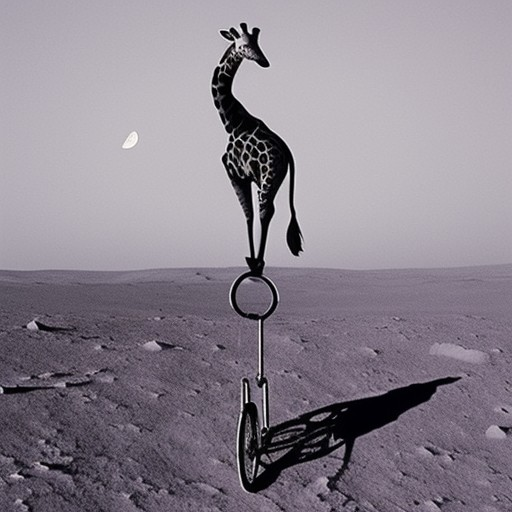
\includegraphics[width=0.5\linewidth]{images/intro/giraffe.png}
    \end{center}
    \caption{Using Stable Diffusion~\citep{rombach2022high} to generate a photo of "a giraffe riding a unicycle on the moon"}
    \label{fig:diffusion_example}
\end{figure}



\subsection{Image Generation}
Image generation has seen phenomenal and almost unbelievable progress in recent years, mainly due to improvements in model architecture, 
increasing model capacity, and increasing the size of training datasets.
In 2013, the Variational Auto-Encoder (\ac{VAE})~\citep{Kingma2014} allowed blurry, low-quality results of images in a particular domain. In 2014,
\ac{GAN}s were introduced, which Yann LeCun, a \ac{DL} pioneer, described as “the most interesting idea 
 in the last 10 years in Machine Learning”. Indeed, the "generator" was trained not alone, but in unison with another network, the "discriminator",
 both trained "adversarially" (their respective objectives are opposing). The \ac{GAN} frenzy lasted until the start of the 2020's, and for the
  first time  allowed truly realistic generations of images in restricted domains, particularly faces. Indeed, the popular website
   \urlstyle{thispersondoesnotexist.com} displayed the uncannily realistic face generations using StyleGan~\citep{karra2019stylegan, karra2020stylegan2}.
    However, \ac{GAN}s struggled with 
   larger and more diverse domains, leaving room for other architectures, like the \ac{ViT}~\citep{esser2021taming, ramesh2021zero, ding2021cogview}.
    Only recently,
   remarkable progress was made with \ac{DDPM}~\citep{ho2020denoising,nichol2021glide, rombach2022high, ramesh2022hierarchical, saharia2022photorealistic}. 
   These models, as we will later see, have a simple loss function and allow stable training even when scaling up their architecture.
   As \ac{DDPM}s quickly made their way to becoming state-of-the-art for various datasets, particularly ImageNet~\citep{deng2009imagenet}, researchers
   started to scale up the models further and train them on massive billion element text-image datasets. The past few years have welcomed
   a true revolution in Image Generation, allowing generation of images which are not only realistic, but also of unprecedented diversity.
   Indeed, a completely imaginary and absurd prompt such as "a giraffe riding a unicycle on the moon" actually produces a  plausible 
   output image, as shown in \ref{fig:diffusion_example}.



   

\subsection{Image Editing}
Before digital photography, photographs were created in multiple steps: first, light interacts with light-sensitive chemicals on 
a camera's film, which produces a \emph{negative} photograph; then, the negative photograph can be developed into a \emph{positive} 
photograph in a darkroom with the help of chemicals. Before digital editing, real-image editing 
consisted in manually manipulating the negative 
photograph before further processing it to develop the positive image. These practices date back to the 1840s, almost 200 years ago.

In contrast, real-image editing with \ac{DL} has a relatively recent history, mainly taking off following the introduction of \ac{GAN}s after 2014.
Image editing has foundations as an Image-to-Image translation problem, where a \ac{DNN} is trained to learn the transformations from 
one domain to another~\citep{isola2017image}. These edits were initially limited to edits akin to style-transfer, like transforming 
photographs to paintings or night images to day images, and often presented visible artifacts.
Over time, image-editing techniques became more elaborate, where the editing operation could change  specific attributes 
(like man$\rightarrow$woman)~\citep{choi2020stargan} or use a user-given text prompt~\citep{li2020manigan}. These methods still struggled with artifacts 
and fidelity to the input image, though, since changes were effected in a fully-convolutional manner. More recently, the latest 
\ac{GAN}s~\citep{karra2019stylegan, karra2020stylegan2} 
were shown to have localized and meaningful editing capabilities via their latent code, allowing semantic edits like man$\rightarrow$woman 
while more faithfully preserving the initial image. Other works perform manipulation of the learned weights within a trained network for 
even more controllable generation~\citep{bau2020rewriting}. Using a pre-trained generative prior, like a \ac{GAN} or \ac{DDPM}, has the advantage 
of leveraging the learned relationships in a large and powerful network. Training an editing network from scratch, however, requires large amounts of data and 
computation power, while only allowing limited types of editing instructions. Moreover, manipulating the internal weights and latent code of a 
pre-trained network typically allows for more natural edits than a trained editing network. However, generalizing these edits to real images is not straightforward, 
as we need an effective way to encode a real image into the network. Moreover, using a pre-trained generative network may limit us to the distribution of the 
training dataset. 
In this thesis, we explore these problems when leveraging
and manipulating the compact representations of pre-trained generative priors to effectuate target editing operations. 

Our use of \ac{DNN}s
for image editing in 2023 can be seen as an amusing echo to the image editing performed almost 200 years ago. Indeed, if the compact negative image 
is seen as the "latent image" of traditional photography, traditional image editing techniques consisted in manipulating this "latent image" before "decoding" 
it into a positive image. Likewise, 
we focus on manipulating the latent vectors of various generative models while striving to push the generated image to be as natural as possible.


\section{Contributions}

Editing real images with \ac{AI} is a unique case where the "artificial" meets "human". 
While a fake image 
which is entirely generated by an \ac{AI} system is trained to be harmonious by the model, an edited image
requires a generation which is not only realistic but also faithful to the original image. This 
tradeoff between \emph{editing success} and \emph{fidelity to the original image} is a recurrent theme which we will see throughout 
our thesis, both to build our methods as well as evaluate them. We tackle several different families of editing operations (attribute editing, 
text-guided editing, and inpainting) and leverage different generative models to accomplish our task. 

Throughout this thesis, we would like the reader to be aware of the three objectives we have when it comes to image editing:

\begin{enumerate}
    \item Fidelity to the input image
    \item High quality output image 
    \item Fidelity to the edit operation 
\end{enumerate}

We approach image editing from several different lenses, which we quickly summarize  here:

\begin{itemize}
      \item \autoref{chapter:magec}: \nameref{chapter:magec}\\
            We first approach real image editing by generalizing \ac{GAN} latent manipulation techniques 
            to real images. Indeed, latent manipulation produces meaningful and realistic edits to 
            generated images, but requires a real image to first be inverted into a \ac{GAN} before applying the same techniques. 
            However, naively inverting an image into a \ac{GAN} produces poor edits of the image. We analyze the reasons for this and we 
            propose a better strategy for \ac{GAN} inversion, with editability as our motivation. The work in this chapter has led to the following 
            conference publication:
            \begin{itemize}
                \item \fullcite{grechka2021magecally}
            \end{itemize}


      \item \autoref{chapter:flexit}: \nameref{chapter:flexit}\\
            While our inversion strategy allowed meaningful edits, it still struggled with 
            out-of-domain images with regards to the pre-trained \ac{GAN}. In this chapter,  we  decide to 
            circumvent inversion altogether and optimize the latent vector of an autoencoder to 
            perform text-given edits. Our method relies on well-studied regularizers to produce a 
            high-quality edited image. The work in this chapter has led to the following 
            conference publication:
            \begin{itemize}
                  \item \fullcite{couairon2022flexit}
            \end{itemize}

      \item \autoref{chapter:gradpaint}: \nameref{chapter:gradpaint}\\
            While the previous work can be flexibally applied to any given image and text-prompt, the 
            lack of a strong generative prior sometimes makes the editing operation fail. In this chapter, 
            we look into the use of using a \ac{DDPM} for the specific task of inpainting. Indeed, we can 
            guarantee fidelity to the input image while producing a high-quality generation thanks to the 
            pre-trained \ac{DDPM}. Our work is currently in submission:
            \begin{itemize}
                  \item \fullcite{grechka_gradpaint}
            \end{itemize}
\end{itemize}




% In this thesis introduction, using layman terms, we describe Artificial Intelligence, and,
% in particular, one of its instances: Deep Learning. Then, we lay out the challenges of this
% thesis and our contributions.

% %\section{Artificial Intelligence}

% \textbf{The idea of thinking machines} began in the previous century, from Karel Çapek's invention
% of the "\textit{robot}" to the 1956's Dartmouth workshop passing by Turing \& von Neumann's
% reflections. Despite suffering from multiple "AI winters" filled with disappointments and
% criticisms, Turing's prediction on the rising importance of \ac{AI} proved to be right as the first
% and the second decades of the XXI century saw the advent of respectively \acf{ML}
% \citep{bishop2006prml} and \acf{DL} \citep{goodfellow2016deeplearningbook}, two major subfields of
% \ac{AI}, related to statistical learning theories.

% Providing \textbf{a definition of \ac{AI}} is difficult, but its foremost domains, \ac{ML} and
% \ac{DL}, can be defined as statistical algorithms that can improve automatically through experience
% and the use of data. These methods are already ubiquitous: speech recognition enabling us to control
% devices remotely \citep{amodei2016deepspeech2}, recommender systems proposing movies according to
% our taste \citep{toscher2009netflixprize}, automatic translation \citep{vaswani2017transformer},
% face recognition \citep{schroff2015facenet}, autonomous driving \citep{sun2020waymodataset}, \etc.
% Less known but still useful applications comprise accelerated physics simulation
% \citep{breen2020threebody}, protein folding prediction \citep{jumper2021alphafold}, molecule
% toxicity estimation \citep{nih2019toxchallenge}, data center cooling
% system \citep{evans2016datacentercooling}, control of the magnetic coils of a nuclear fusion reactor
% \citep{degrave2022nuclearreactor}, \etc.

% \ac{AI} is increasingly more important in our daily lives with some applications raising
% \textbf{ethical concerns}: face recognition biased towards some populations
% \citep{grother2019facerecoethic}, loan grants \citep{anglekar2021loangrantml}, medical diagnosis
% \citep{lazzazabal2020medicalbias}, justice advice \citep{russel2020justicefairness}, biased chatbots
% \citep{sheng2019lmbias}, \etc. Therefore, we must pay a particular interest in the potential impact
% of this new technology. Towards this goal, people from diverse backgrounds must participate in the
% creation of such technology, and standardization bodies \citep{tommasi2021fairness} should advise
% what types of \ac{AI} systems can be used in which scenarios \citep{gebru2019aiethichandbook}.

% \section{PhD Thesis Context}

% I now contextualize my thesis with relation to my sponsor, how it influenced our research, and what
% challenges we have aimed to tackle.

% \paragraph{Heuritech} This thesis was sponsored by the Parisian startup
% Heuritech\footnote{\url{https://heuritech.com}} as a \textit{CIFRE PhD}. The company analyzes social
% networks such as Instagram and Weibo, recognizes the clothes in pictures, estimates
% volumes of fine-grained types of garments, and finally forecasts future trends. The company's
% \acf{CV} models must recognize an ever-growing number of entities from features (\eg knitted, blue
% color, short cut) to brand models (\eg Nike Air Max, Adidas Stan Smith, Puma Suede). This
% requirement leads to two problems: \textbf{(1)} the time spent to re-train a model is growing
% linearly, and \textbf{(2)} learning a new entity can incur a performance loss on previously learned
% entities.

% \paragraph{Continual Learning} is a field that emerged in the 1990s but saw renewed interest only
% very recently around the second half of the 2010s. The goal is to deal with datasets that evolve
% through time. This evolution can take many forms, including adding new entities to predict in a
% classification task (\eg learning sneaker brands, then high-heel brands) or adding samples from new
% sources (\eg commercial photoshoot then images from social media). Unfortunately, current
% State-of-the-Art models struggle to learn continually from new data without losing performance on
% previously seen data. This loss is so critical that the literature nicknamed it ``\textit{catastrophic
%       forgetting}'' \citep{robins1995catastrophicforgetting,french1999catastrophicforgetting}. Multiple
% methods can reduce this forgetting, including rehearsal and constraints. Rehearsal involves
% reviewing previously learned knowledge, as a human student would \textit{rehearse} the last
% semester's course. However, this rehearsal is often limited in order to reduce computational cost
% and because past data may not always be available for a variety of reasons, including privacy. On
% the other hand, constraints enforce the model to keep a similar \textit{behavior} as it learns new
% concepts, but defining the optimal constraint is not trivial.

% \section{Contributions}

% This PhD thesis is structured around solving catastrophic forgetting in continual settings. We
% considered various specific situations and approaches declined in several chapters:

% \begin{itemize}
%       \item \autoref{chapter:regularization}: \nameref{chapter:regularization}\\
%             We first propose strategies to tackle catastrophic forgetting in deep neural neworks in
%             the context of the image classification. Our main goal is to constrain the evolution of the
%             network parameters during the continual training to be relatively rigid while also
%             avoiding completely freezing the network. The work in this chapter has led to two
%             conference publications:
%             \begin{itemize}
%                   \item \fullcite{douillard2020podnet}
%                   \item \fullcite{douillard2020ghost}
%             \end{itemize}

%       \item \autoref{chapter:segmentation}: \nameref{chapter:segmentation}\\
%             Then, we extend our focus to the task of semantic segmentation. We show that this
%             context brings new challenges, and we propose multiple complementary approaches to tackle
%             them. The work in this chapter has led to one conference publication and one submission
%             to a journal:
%             \begin{itemize}
%                   \item \fullcite{douillard2020plop}
%                   \item \fullcite{douillard2021objectrehearsal}
%             \end{itemize}

%       \item \autoref{chapter:dynamic}: \nameref{chapter:dynamic}\\
%             Finally, in our last chapter, we consider the impact of the neural network architecture
%             for continual learning and in particular propose using the recent Transformer. The work
%             in this chapter has led to a conference publication:
%             \begin{itemize}
%                   \item \fullcite{douillard2021dytox}
%             \end{itemize}
% \end{itemize}


\cleardoublepage

\acresetall % flush acronyms so they are redefined completly when first used

% to remove biber: sudo rm -r /var/folders/qh/d5q46r4n40334yrtc9tqf8nw0000gn/T/par-6173796167726563686b61/cache-e34ad03908a9c47f3411cdb5bf7054398afc2974

\chapter{Related Work}
\label{chapter:related}

% \minitoc


\chapterwithfigures{\nameref*{chapter:related}}
\chapterwithtables{\nameref*{chapter:related}}

\ifthenelse{\boolean{skipRelated}}{\endinput}{}

% related work - 
% 2.1 NN 
% 2.2 generatif 
%       - talk about stylegan quickly 
% 2.3 edition ; 
%       -> text 2 image GAN 
%       -> DALL-E 
% 2.4 position ; where are we 

% --> we shouldn't go into details

% GAN work general
% transformer 
% diffusion model 
% image 2 image models 

% MAGEC - 
% related work 
% - latent manipulation 
% - stylegan 

% maybe not related work; but "context" 
% grosse figure avec h; z 

% je peux avoir 2 niveaux de granularite pour parler de la meme chose ! 

% je peux reprendre dans le chapitre magec 

% faire un petit git pour pusher 
% ou push sur nextcloud


% d'ici un truc a mettre 

% jury : 
% - Stéphane Lathuilière -> ca va etre pertinent 
% - Karteek Alahari
% - david picard https://davidpicard.github.io/
% - patrick perez - valeo 
% - Laure -> 
% - on invitera Antoine pour le jury 
% - valeo 2j; tout le monde soit la le jeudi; metro courset
% - l'autre centre valeo creteil 
% - le mieux c'est de faire un talk 
% - septembre 


\todo{add note on GigaGAN (CVPR 2023) and StyleGANXL}


In this chapter, we will first give a quick overview of Neural Network Learning before 
going into the details of the separate families of generative networks which were used in our work. 
Then, we will discuss different approaches to image editing. Finally, we will discuss our contributions 
and where our work situates among the described context of existing works. 

\section{Neural Network Learning}

A \ac{NN} can represent any parameterized and differentiable mapping function 
$f_\theta : \mathcal{X} \rightarrow \mathcal{Y}$ 
between an input space $\mathcal{X}$ and an output space $\mathcal{Y}$. Each \emph{layer} of the 
\ac{NN} is a differentiable mathematical function. A \ac{DNN} refers to defining many layers 
(with many learnable parameters) in this network, allowing us to represent extremely complicated functions.
The application and training of these models is referred to as \ac{DL}.
In the case of \emph{supervised learning}, we have access to a ground-truth dataset $\mathcal{D} = 
\{(x_1, y_1), ..., (x_N, y_N)\}$ which associates every datapoint $x_i \in \mathcal{X}$ to its
ground-truth label $y_i \in \mathcal{Y}$. In the case of \emph{unsupervised learning}, we only 
have access to unlabelled training data $\mathcal{D} = \{x_1, ..., x_N\}$. 
We define a differentiable loss function $\mathcal{L}$ which estimates the error of the  \ac{NN}
prediction prediction $f_\theta$. Because the \ac{NN}
is fully differentiable, we are able to calculate the gradient of the loss function with respect 
to the \ac{NN} parameters $\theta$, and thus iteratively optimize them. At the core level,
the iterative algorithm which \emph{trains} a \ac{NN} is called \emph{Gradient Descent},
 although many variants have been introduced to improve or speed up training \citep{ruder2016overview}.

\ac{DL} is used today in multitudes of fields and applications. Any data which can be numerized 
can then be used to train \ac{DNN}s. In the particular case of \ac{CV}, we aim to build models 
which treat image data. In this case, $\mathcal{X}$ are images, represented as 
$\mathrm{n} \times \mathrm{m} \times \mathrm{c}$ matrices in which each value is an integer 
between $0$ and $255$. The number of channels $mathrm{c}$ is $1$ in the case of black and white 
images and $3$
in the case of colored images. Historically, handcrafted features were extracted from images and 
then aggregated in an approach similar to "bag of words" \citep{lowe2004distinctive, ahonen2004face, dalal2005histograms}
before inserted in a shallow network which calculated the prediction. In 2012, AlexNet \citep{krizhevsky2012imagenet}
became the first deep \ac{CNN} to win the \ac{ILSVRC} competition for classifying diverse images.
Here, small "kernels" of trainable weights were used throughout the network, learning hierarchical 
features without any need of handcrafting features.
Improvements in coming years came with prominent architectures like VGG \citep{simonyan2014very}, which 
had a deeper architecture with smaller kernels 
and ResNet \citep{he2016resnet}, which introduced residual connections. In recent years, 
Visual Transformer architectures \citep{dosovitskiy2020vit, touvron2021deit, chen2022pali} became state-of-the-art for the task of 
image classification. Like their \ac{NLP} counterparts, Visual Transformers treat images 
as a sequence of "tokens" - created by extracting and flattening patches across the image before 
learning their deeper embeddings through their signature "attention" mechanism. 


% \todo{computer vision context; deep learning. donner des exemples ou 
% $f_\theta(x)$ ou x c'est des images. maybe cite here bow, alexnet, etc. vgg 
% resnet. and then transformers, vit. general ou x est l'image}

% \todo{maybe change the figure with the $z$ and $x_n$ alignes}

% \todo{finish conditional gan's here, but maybe have a section on conditional models in general
% maybe change the general schema vers z.}

% \todo{change the citations so that they will be in a different color. 
% otherwise it's not so clear.}

% \todo{go quick on the equation for ddpm, big figure for ddpms. latent diffusion 
% can go to prominent diffusion models.}


\section{Generative Models}

Generative Models model the distribution $p(x)$ of a given dataset $\mathcal{D}_{\mathcal{X}}$ and provide a 
way to generate new data points from this distribution. In this section, we will first investigate 
the various generative models from the scope of \emph{unconditional generation} before describing their 
conditional counterparts. In the unsupervised setting, we only have access to a 
given  dataset $\mathcal{D}_{\mathcal{X}}$ and we wish to model $\mathcal{D}_{\mathcal{X}}$'s distribution with a 
\ac{DNN}. Although we do not have ground-truth labels, we must still define a loss function in order to 
backpropogate through the network and update its parameters, as described in the section above. The 
different families of generative models each propose to optimize a distinct loss function which 
have their advantages and disadvantages. 

We specifically focus on image generation, particularly high-quality
image-generation. Although generative models can be applied to other forms of data as well, like 
numerical data, text, or speech, it is important to keep in mind that in the context of this thesis, 
we are dealing with very high-dimensional data (in the case 
of a $500\times500$ image, there are $750000$ dimensions represented with 8-bit values). Thus, models which assume 
that data follows a pre-defined distribution, like Gaussian Mixture Models 
\citep{em_algoo}, are 
ineffective for our goal. Indeed, \ac{DNN}s specfically have had the most success modeling 
this complicated form of data. In this work, we specifically use three families of different generative models:
\ac{VAE}s, \ac{GAN}s and \ac{DDPM}s. These families have had great success in the task of 
image generation and we use these three families in our work. Figure \ref{fig:gen_models}
summarizes these the architectures of these families. It's worth noting that other generative models have also had 
success at the task of image generation, such as Normalizing Flows \citep{rezende2015variational, dinh2014nice}
 and particularly autoregressive models based on Visual Transformers \citep{esser2021taming, ramesh2021zero, ding2021cogview, gafni2022make, yu2022scaling}
but these models are out of the scope of our thesis. 

\begin{figure}[tb]
      \begin{center}
          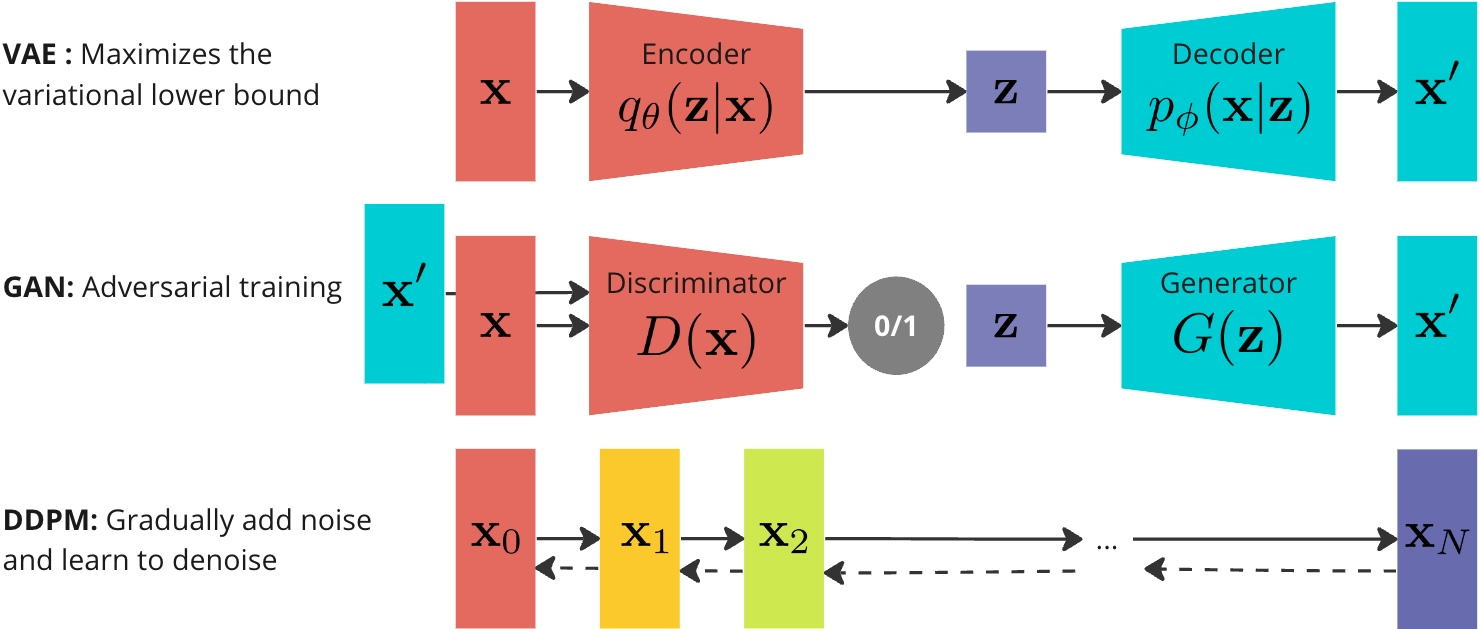
\includegraphics[width=1.0\linewidth]{images/related/generative_models_overview.jpg}
      \end{center}
      \caption{Overview of three families of generative models used in this work.}
      \label{fig:gen_models}
  \end{figure}


\subsection{Variational Auto-Encoders}\label{section:chapter1_variational_auto_encoders}

Introduced by  \cite{Kingma2014} and \cite{pmlr-v32-rezende14}, \ac{VAE}s are based on the variational 
inference framework. This framework will be presented here and then later be brought to the context of \ac{DL}.

\paragraph{VAE Framework}
Let's consider a dataset of observations $x \in \mathcal{D_X}$, a prior distribution of unobserved latent 
variables $p(z)$. The joint probability of this model can be written as $p(x,z) = p(x|z)p(z)$. The goal of 
\emph{variational inference} is to \emph{infer} good values of the latent variables and calculate the posterior
(intractable) $p(z|x)$. 

% Using Bayes theorem, we have:
% \begin{equation}
%       p(z|x) = \frac{p(z, x)}{p(x)}
% \end{equation}
% However, $p(x)$ is intractable, since we would need to compute it using all possible configurations of latent 
% variables. Thus, we need a way to approximate this posterior. 


Variational inference approximates the posterior with a family of distributions, typically multivariate 
Gaussian distributions, noted as $q_\lambda(z|x)$. To measure the similarity between the variational 
posterior $q_\lambda(z|x)$ and the true posterior $p(z|x)$, we can use the \ac{KL} divergence which measures
the similarity between two distributions. However, $\mathrm{KL}(q_\lambda(z|x) || p(z|x))$ is again intractable.

% We thus want to minimize:

% \begin{equation}
%       \mathbb{KL}(q_\lambda(z|x) || p(z|x)) = \mathbb{E}_q[\log q_\lambda(z|x) ] - \mathbb{E}_q[\log p(z|x) ] + \log p(x)
% \end{equation}

% However, this term is intractable because it again depends on $p(x)$.

The marginal log-likelihood can be decomposed as follows:

\begin{equation}
      \label{VAE_px_definition}
      \log p(x) = ELBO(\lambda) + \mathrm{KL}(q_\lambda(z|x) || p(z|x))
\end{equation}

with 

\begin{equation}
      ELBO(\lambda) = \mathbb{E}_{q_{\lambda(z|x)}}[\log p(x|z)] - \mathrm{KL}(q_\lambda(z|x) || p(z))
\end{equation}

Because the \ac{KL} divergence is always positive,  minimizing the right term in 
Eq.~\ref{VAE_px_definition} (which is intractable) is equivalent to maximizing $ELBO(\lambda)$, which is tractable. 
Indeed, $ELBO(\lambda)$ is a lower bound on the the marginal log-likelihood of the observed data $\log p(x)$.

\paragraph{DNN Context}
In the context of \ac{DL}, we parameterize the approximate posterior $q_\theta(z|x)$ with an encoder network which 
takes as input an image and outputs the parameters to a probability density. This 
is typically a multivariate Gaussian distribution, defined by a mean $\mu_\theta$ and standard deviation $\sigma_\theta$. Sampling from this 
distribution gives us a latent vector $z$. Similarly, we parameterize the likelihood $p_\phi(x|z)$ with a decoder 
(generative network), which takes as input a latent vector $z$ and outputs parameters of the data distribution.
For practical purposes, this distribution is typically a set of independent Bernouilli parameters or a multivariate 
Gaussian with fixed variance. In this way, the decoder
network simply outputs the reconstructed image directly.
The parameters $\theta$ and $\phi$ are the weights to the 
encoder and decoder respectively, and can be optimized via gradient descent. Note that when sampling a 
latent vector $z$ from the output given by the encoder, we perform a \emph{reparametrizaton trick} which 
allows us to backpropagate through the encoder network. This consists in sampling a random vector 
$\epsilon \sim \mathcal{N}(0, I_d)$ and then reparameterizing to obtain the latent vector $z$ with 
$z = \mu_\theta +  \sigma_\theta * \epsilon $. The basic architecture can be visualized in the 
first row of Figure \ref{fig:gen_models}.

% \begin{figure}[tb]
%       \begin{center}
%           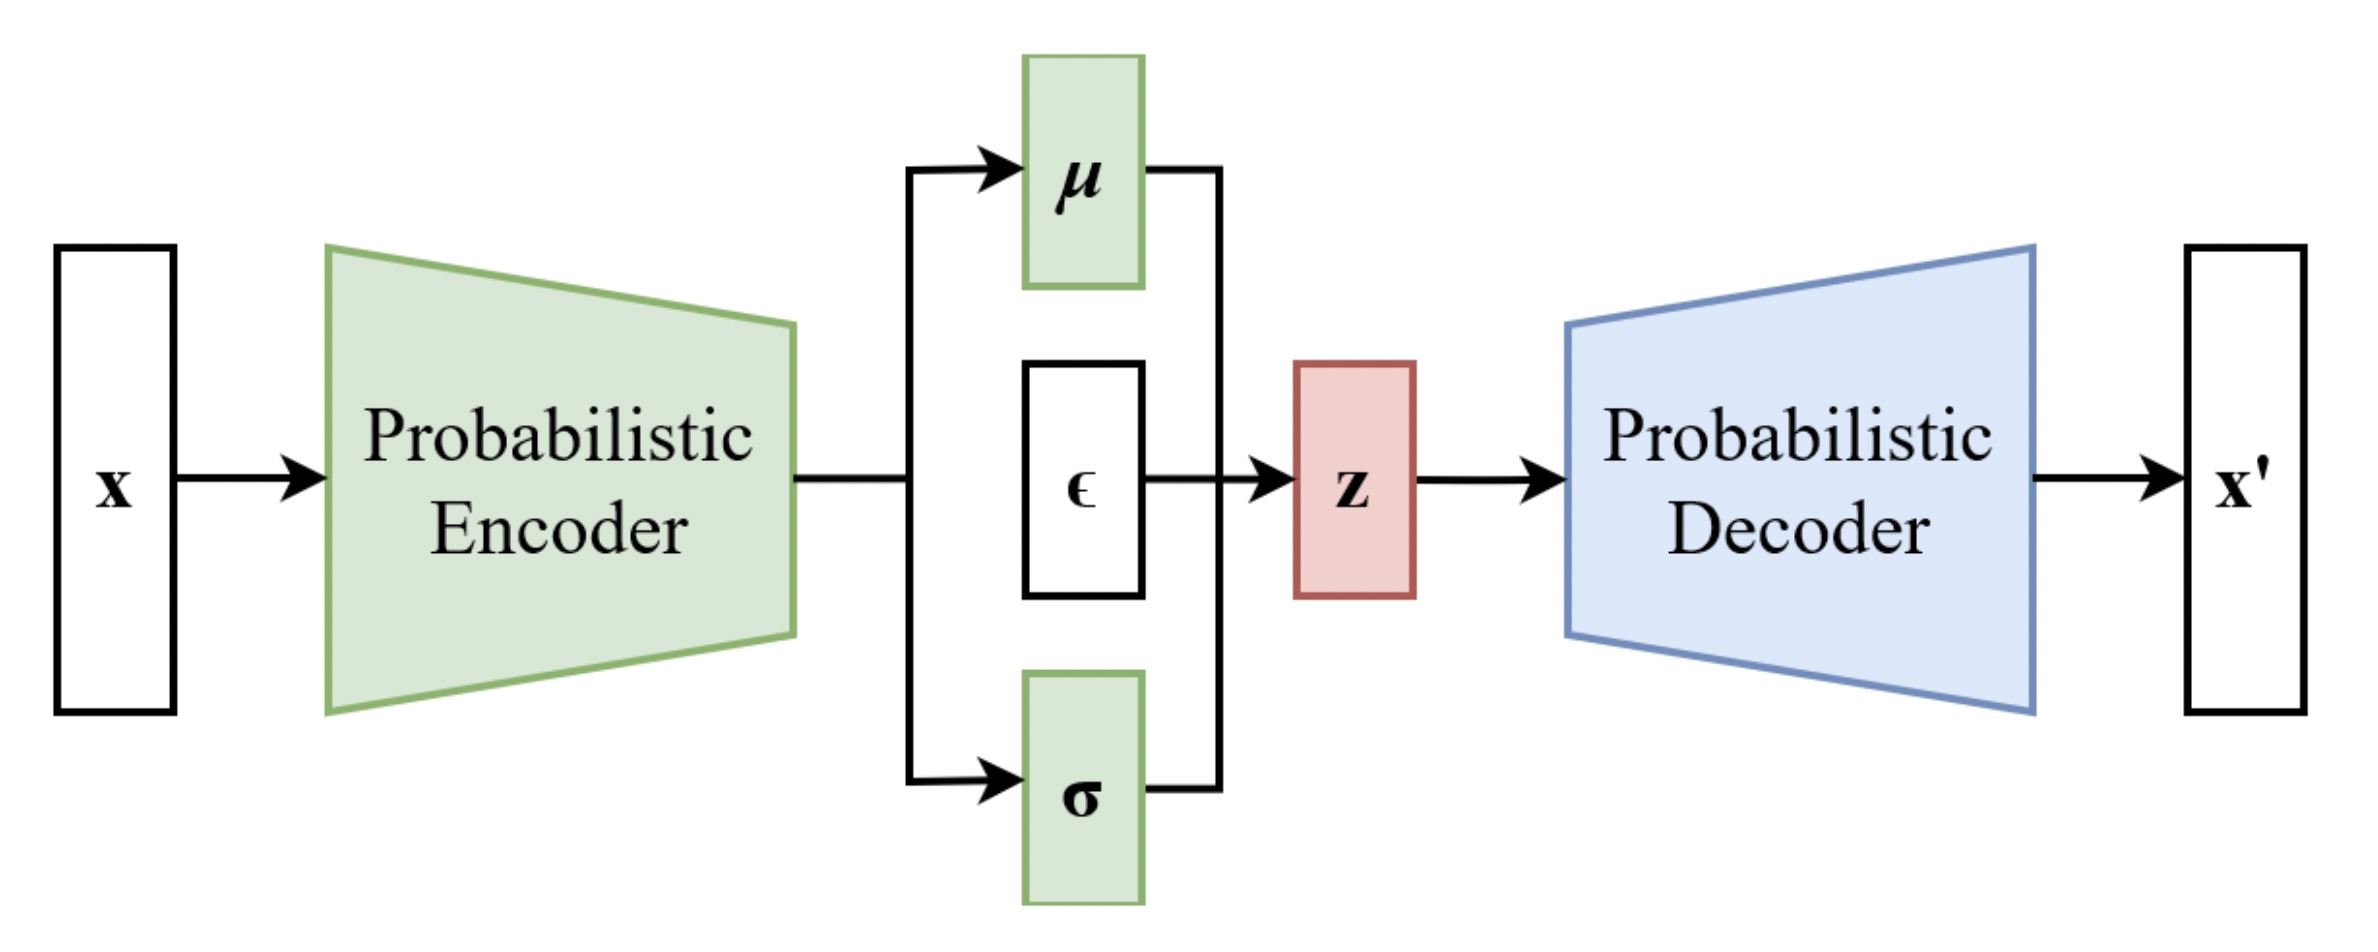
\includegraphics[width=1.0\linewidth]{images/related/vae.jpg}
%       \end{center}
%       \caption{Basic VAE architecture, using reparameterization trick.}
%       \label{fig:vae}
%   \end{figure}

We minimize the following loss function:

\begin{equation}
      L = \frac{1}{N}\sum_{i}^{N}l_i
\end{equation}

where 

\begin{equation}\label{eq:vae}
      l_i(\theta, \phi) = -ELBO(\theta, \phi) = - \mathbb{E}_{q_\theta(z|x_i)}[\log p_\phi(x_i | z)] + \mathrm{KL}(q_\theta(z|x_i)||p(z))
\end{equation}

and $N$ is the number of datapoints. 

The left term can be seen as the \emph{reconstruction loss}, which refers to how well 
the \ac{VAE} manages to reconstruct a given image. The right term can be seen as a 
regularizer which encourages the learned latent space to be meaningful. Without this 
regularizer, the encoder could assign a unique location for each image in the dataset. 
Although this would be easier to decode, the learned representation of the latent 
would not be \emph{meaningful}, which is one of our goals when learning this 
deep representative space.
 A meaningful latent space implies that two datapoints close 
in the latent space are also close in the image space. 


\paragraph{Disentanglement}\label{sec:disentanglement}

In fact, \cite{higgins2017betavae} show that when putting more penalty on the 
the \ac{KL}-divergence term in Equation \ref{eq:vae}, known as $\beta$-VAE, the \ac{VAE}
produces \emph{disentangled} representations. Disentanglement refers to a learned 
latent space in which each latent factor is mapped to an 
independent generative factor. For example, in a disentangled represenation, 
 one latent factor could control rotation 
while another one could control size. A disentangled latent space can be especially attractive 
in the case of image editing, which will be discussed later in \ref{subsection:latent_space_manipulation}.

\subsection{Generative Adversarial Networks}\label{sec:gans}

% \todo{talk about BigGAN and imagenet}

We will now introduce \ac{GAN}s, a framework introduced by \cite{goodfellow2014gan}
which has been become a core component in image generation and image editing applications. 


In contrast with \ac{VAE}s, \ac{GAN}s do not explicity model the probability 
distribution of the data $p(x)$. Instead, \ac{GAN} use two networks, the generator $G$ 
and the discriminator $D$ which are trained together adversarily. Similarly to 
\ac{VAE}, we use a latent space ${z \in \mathcal{Z}}$ which will be used as input for the 
generator network. Unlike \ac{VAE}s, this latent space is not learned, and is 
typically defined as $\mathcal{N}(0, I_d)$, with $d$ the dimension of the latent space. 

Concretely, the 
objective function of \ac{GAN}s is posed as a zero-sum game between $D$ and $G$, defined 
as follows:
\begin{equation}\label{eq:gan_objective}
      \min_{G}\max_{D}\mathbb{E}_{x\sim p(x)}[\log(D(x))] + \mathbb{E}_{z\sim p(z)}[\log(1 - D(G(z)))]
\end{equation}

For the discriminator, the goal is posed as a binary classification problem: 
correctly classify the real images from $p(x)$ as well as the fake images generated 
from $G(z)$. The generator has the opposite objective and "wants" to produce 
images that cannot be easily classified by the discriminator. 

Minimizing Equation \ref{eq:gan_objective} is equivalent to minimizing the \ac{JSD} between the 
distribution of real images and distribution of fake images. However, 
training GANs in practice is not straightforward, for reasons we will examine here.

\subsubsection{GAN Architecture}\label{sec:gan_architecture}
When referring to \ac{GAN}s, we typically refer 
to the training mechanism using the zero-sum \emph{GAN loss} (Equation \ref{eq:gan_objective}). This requires 
some generative network and a discriminator network trained jointly, but there is no further constraint on the 
architecture used by a \ac{GAN}.  Indeed, a \ac{VAE}'s decoder architecture can be practically identical
to a \ac{GAN}'s generator network, both transforming a latent vector $z$ into an image. Similarly, the 
discriminator can simply ressemble a CNN-classifier architecture. 
For this reason, there is nothing stopping us from having hybrid architectures which combines the 
typical encoder-decoder of a 
\ac{VAE} with a discriminator and a \ac{GAN} loss, as has been done by several works \citep{larsen2016autoencoding, 
donahue17iclr, dumoulin17iclr, xian2019f, esser2021taming}. In the case of images, Figure \ref{fig:dcgan} shows a typical \ac{GAN} architecture based 
on a \ac{CNN}, coined \ac{DCGAN} \citep{dcgan}. This basic architecture uses upsampling blocks 
(composed of deconvolutional layers) for the generator and downsampling blocks (composed of convolutional layers)
for the discriminator, which further works build off from. 

\begin{figure}[tb]
      \begin{center}
          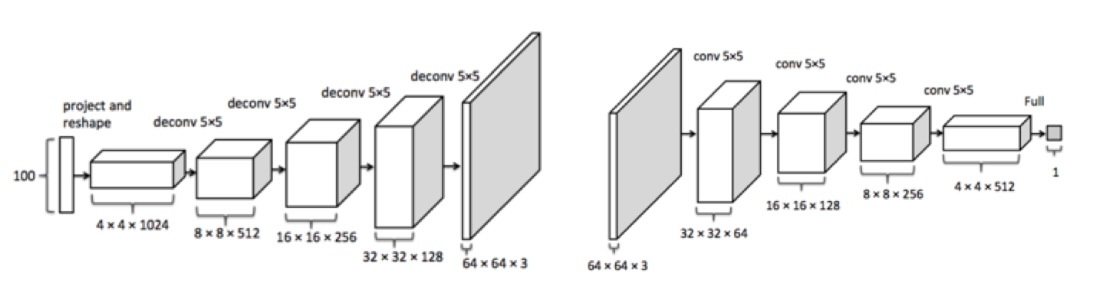
\includegraphics[width=1.0\linewidth]{images/related/dcgan.jpg}
      \end{center}
      \caption{DCGAN architecture. Generator (left) uses upsampling blocks with deconvolutional layers while the discriminator 
      (right) is a mirror image of the generator and uses downsampling blocks composed of convolutional layers.}
      \label{fig:dcgan}
  \end{figure}


\subsubsection{GAN Weaknesses}\label{subsubsection:gan_weaknesses}

\minipar{Training Instability}
In theory, we can expect to optimize Equation \ref{eq:gan_objective} by first optimizing $D$ 
optimally before optimizing $G$. In practice, however, training \ac{GAN}s is effectuated 
by alternating gradient descent steps to the discriminator and generator. 
However, GANs are prone to important training 
instability. 

One of the most notable issues when optimizing Equation \ref{eq:gan_objective} by alternating 
gradient descent steps is training collapse due to a too-strong discriminator. \cite{arjovsky2017towards}
shows that in the case of image generation, a "perfect" discriminator exists which can perfectly 
separate real data from fake data. What's worse, as the discriminator gets stronger, 
 the gradients  given to the generator will vanish \citep{arjovsky2017towards}. 
 This means, of course, that training collapses, since the generator can no longer improve. 
 It's important to note that this gets exacerbated in the case of high-resolution synthesis. 
 Indeed, while high-resolution images improves discriminability \citep{pmlr-v70-odena17a}, high-resolution 
 synthesis becomes a harder task for the generator \citep{karras2018progressive}. Moreover, in the case of 
 high-resolution synthesis, the size of the mini-batch must be smaller (since the images are more memory-intensive)
 and thus the generator has even guidance from the gradients. The \ac{GAN}'s training stability 
and the \ac{GAN}'s capacity to generate high-resolution images thus goes hand-in-hand. Although the 
reverse problem could also occur in practice (a strong generator which too-easily tricks the discriminator, causing 
the discriminator "stuck" during learning), 
this occurs less often given the fact that the discriminator's job is inherently easier.

\minipar{Mode Collapse} Mode collapse refers to the generator collapsing to only produce one sample or one family of
similar samples. In this case, a single genered sample which is classified as realistic by the discriminator will 
push the generator towards this sample. The adversarial nature of a \ac{GAN} often pushes it to drop modes which are 
deemed less realistic.

\minipar{Unstructured latent space}
Because the latent space is fixed instead of learned, the latent space of a GAN can be unstructured 
and typically entangled. Although not problematic in itself, it can be prohibit or limit 
fine-grained control for generation or manipulation.

\minipar{No inference for z} Because a \ac{GAN} typically lacks an encoder network (with the exception of hybrid \ac{VAE}s/\ac{GAN}s
as mentioned in \ref{sec:gan_architecture}), we cannot easily obtain the latent \ac{GAN} code 
corresponding to a real image. This makes high-level image editing problematic. 

The works and techniques descibed below ultimately allowed \ac{GAN}s to become state-of-the-art in image synthesis.


\subsubsection{GAN Improvements}

We will now discuss some recent advances which address the aforementioned weaknesses as well as the 
recent works which finally allowed very high-resolution synthesis.

\minipar{Non-saturating GAN loss} The non-saturating GAN loss, introduced in the original \ac{GAN}
paper \citep{goodfellowgans} changes the objective of the 
generator from Equation \ref{eq:gan_objective} to:

\begin{equation}\label{eq:non_saturating}
      \min_G \mathbb{E}_{z \sim p(z)}[-\log(D(G(z)))]
\end{equation}

This reframes the initial goal posed by Equation \ref{eq:gan_objective}. Instead of minimizing the 
probability that the generated samples are 
classified as fake, Equation \ref{eq:non_saturating} maximizes the probability that the generated 
samples are real. This objective provides stronger gradient information to the generator early in 
training and aims to treat the vanishing gradients problem evoked above. Although this change in 
objective does indeed help for vanishing gradients, gradients still become very noisy with little
value to the generator when the discriminator becomes too strong \citep{arjovsky2017towards}.


\minipar{Minibatch Discrimination}
Minibatch discrimination, introduced by \cite{improved_techniques_gans}, consists in providing 
extra information to the discriminator regarding the variety of the samples in the current mini-batch. 
Concretely, for a single sample, we calculate its distance (in a feature space) to all the other samples, 
 sum these distances and concatenate this value to the generated sample $x_i$. Other work uses a variant of 
 this by performing standard deviation in the feature space and concatenates these values to the input of 
 the discriminator \citep{karras2018progressive}. Because the discriminator will 
 have access to extra information (very small distances correlate with fake samples), the generator will 
 be encouraged to produce more diverse samples. However, this approach depends on the batch size, which, 
 in the case of high-resolution synthesis, is quite low to accomodate the memory constraints of large images.
 Moreover, it is not immune to the \ac{GAN} dropping some modes. 

 \minipar{Spectral Normalization} Introduced in \cite{miyato2018spectral}, spectral normalization 
 consists in constraining the weights of the discriminator during training. This improves 
 gradient flow during training and helps stability of training.

\minipar{Progressive Growing of GANs}\label{par:progressive_growing}
In 2017, Karras introduced \ac{PGGAN} \citep{karras2018progressive}, which further tackles GANs' instability problems 
specifically for the goal of high-resolution image resolution. This was the first GAN architecture which successfully 
managed to generate high-quality images of $1024 \times 1024$ resolution. The intuition is straightforward: instead 
of brutally generating high-resolution images which is prone to heavy instability for the reasons mentioned above,
 the generator and discriminator should be trained 
\emph{progressively} from low-resolution generation to high-resolution generation. Figure \ref{fig:pgan}
shows the training mechanism for this architecture.
 The generator and discriminator, mirror architecures of 
each other, are first trained to successfully generate $4 \times 4$ resolution images. This is an easy 
task for the generator, and is successfully trained without much training difficulty. When training is 
complete, another upsampling and downsampling block are respectfully added to the 
generator and discriminator. 
At each new addition of a new block, the generation gradually blends a simple nearest-neighbor 
upsampling of the previous layer with the generation of the newly trained network. As training converges (visually or 
by some pre-defined metric), a new block of layers are added to the discriminator and generator. Because at each new 
addition of an upsampling block, the generator's weights are already at decent starting points, 
the gradients from the discriminator are more likely to be able to guide the generator in the right direction.

Later work \citep{karnewar2020msg, karra2020stylegan2} builds off this framework in a single 
architecture which implicitly performs progressive-growing without explicitly changing the architecture at each new 
resolution adition. 

\begin{figure}[tb]
      \begin{center}
          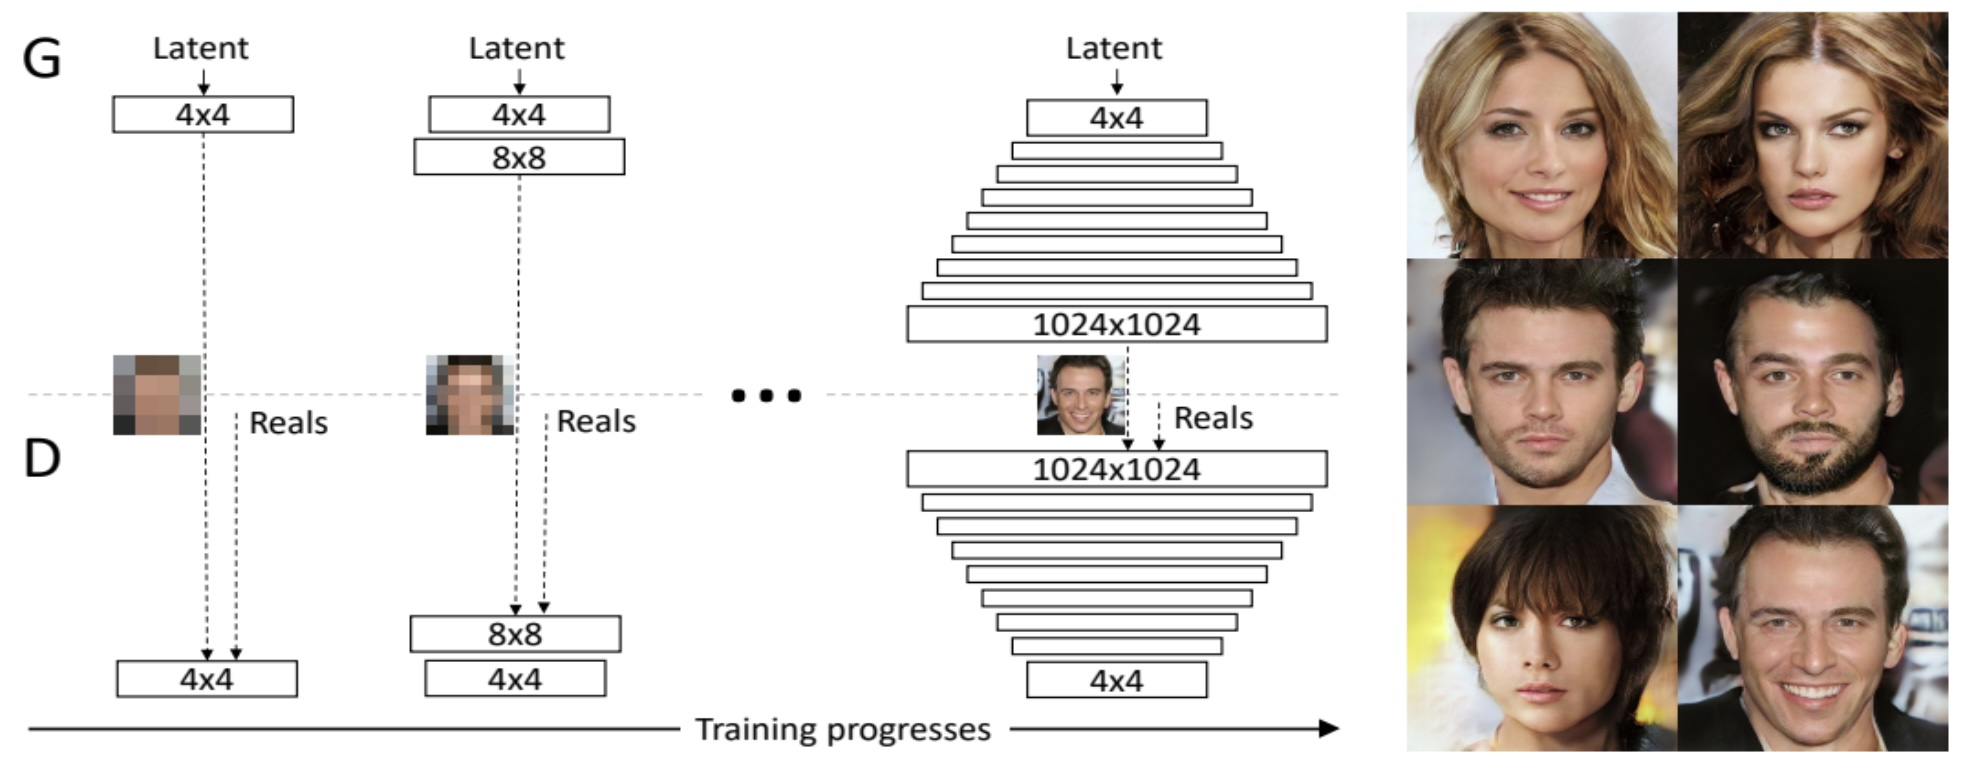
\includegraphics[width=0.7\linewidth]{images/magec/pgan.jpg}
      \end{center}
      \caption{Progressive Growing of GANs. Figure taken from \cite{karras2018progressive}}
      \label{fig:pgan}
  \end{figure}
  

\minipar{A learned and disentangled latent-space}\label{par:latent_space}
Introduced in 2020, StyleGAN \citep{karra2019stylegan} and later StyleGAN2 \citep{karra2020stylegan2}
revolutionized \ac{GAN} synthesis by introducing a new latent space which is learned, rather than the 
typical fixed $\mathcal{N}(0,1)$. Figure \ref{fig:stylegan} summarizes this architecture. We define a 
simple \ac{MLP} network which maps the mapping latent vector from the $\mathcal{N}(0,1)$ space to a new 
learned $\mathcal{W}$ space. This latent code is first projected to another space (the $A$ blocks 
in Figure \ref{fig:stylegan}) and
 then modulates the feature maps via \ac{AdaIN} layers \citep{huang2017arbitrary}, given by the following 
 equation:

 \begin{equation}
      \text{AdaIN}(\mathbf{x}_i, \mathbf{y}) = \mathbf{y}_{s, i}\frac{\mathbf{x}_i - \mu(\mathbf{x}_i)}{\sigma(\mathbf{x}_i)} + \mathbf{y}_{b,i}
 \end{equation}

where $\mathbf{x_i}$ is the $i^{\text{th}}$ feature map in the current layer and $\mathbf{y}$ is 
the learned style parameters for the current block. 

Because each feature map is normalized via the \ac{AdaIN} operation, only the current style at the 
current scale-specific block controls the modification at this level. To further encourage 
styles to localize, \cite{karra2019stylegan} performs \emph{mixing regularization} during training, 
where two different latent codes $\mathbf{w}_1$ and $\mathbf{w}_2$ are mixed at some crossover point 
when synthesizing an image. Moreover, the learned latent 
space naturally encourages disentanglement of high-level image features. This localized latent space
allows a truly controllable image synthesis. Observe 
Figure \ref{fig:stylegan_styles} for example, which shows that by mixing two different style codes 
$\textbf{w}_1$ and $\textbf{w}_2$ (which respectfully generate image $A$ and $B$
through StyleGAN) 
at some cross-over point, we can transform $A$ using coarse, 
medium, or fine-grained styles from $B$. 

In later work, \cite{karra2020stylegan2} improves upon this work by improving the 
architecture, improving the modulation and demodulation scheme of \ac{AdaIN} and adding 
\emph{perceptual path regularization} for even more smoothness in the latent space. 
This encourages for small changes in the latent space to produce small changes in the 
image space. With these improvements, StyleGAN2 quickly became the state-of-the-art 
in image generation for constrained datasets like faces \citep{celeba,karras2018progressive},
 bedrooms and animals \citep{lsun} for many years to come. Moreoever, with its 
 powerful latent space, StyleGAN2 opened the door for many works on image editing, 
 more of which will be discussed in \ref{section:image_editing}.
 

\begin{figure}[tb]
      \begin{center}
          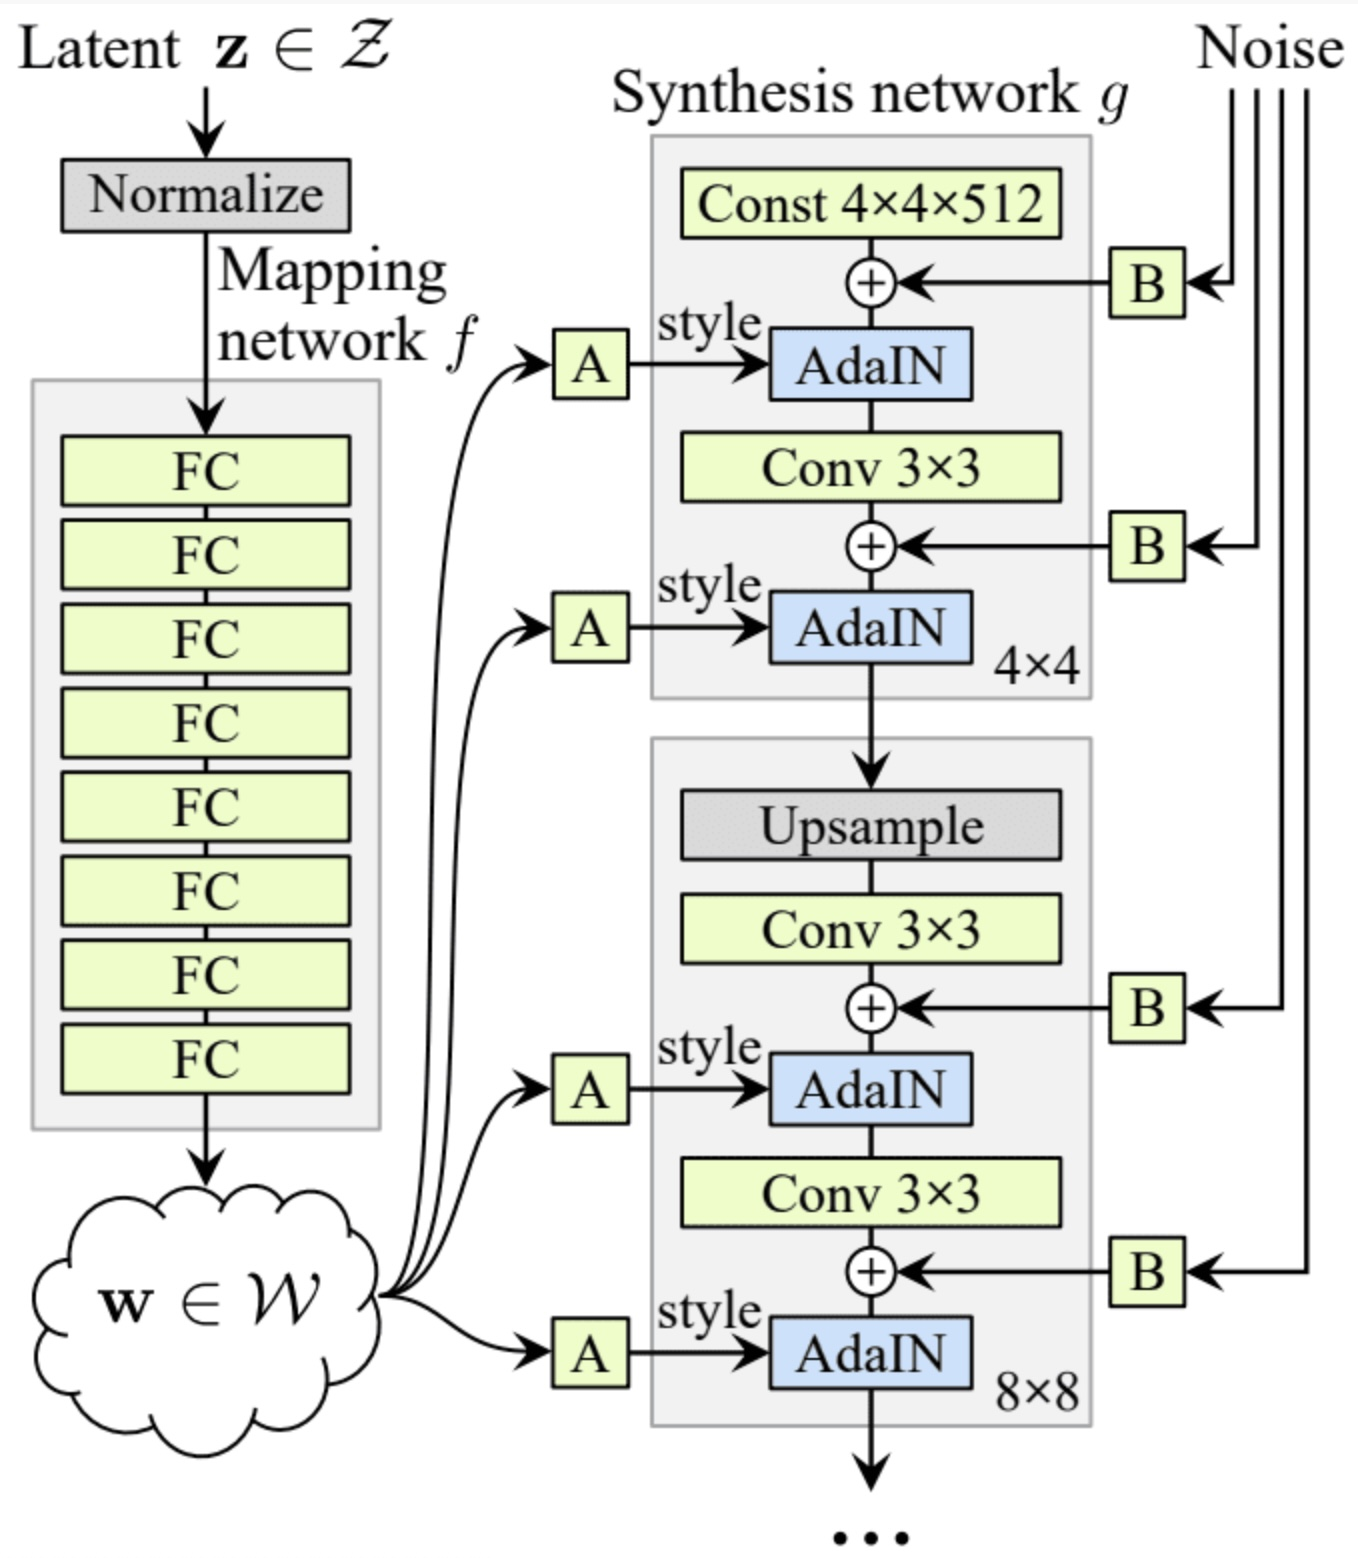
\includegraphics[width=0.5\linewidth]{images/related/stylegan.jpg}
      \end{center}
      \caption{StyleGAN architecture. Figure taken from \cite{karra2019stylegan}.}
      \label{fig:stylegan}
  \end{figure}

  \begin{figure}[tb]
      \begin{center}
          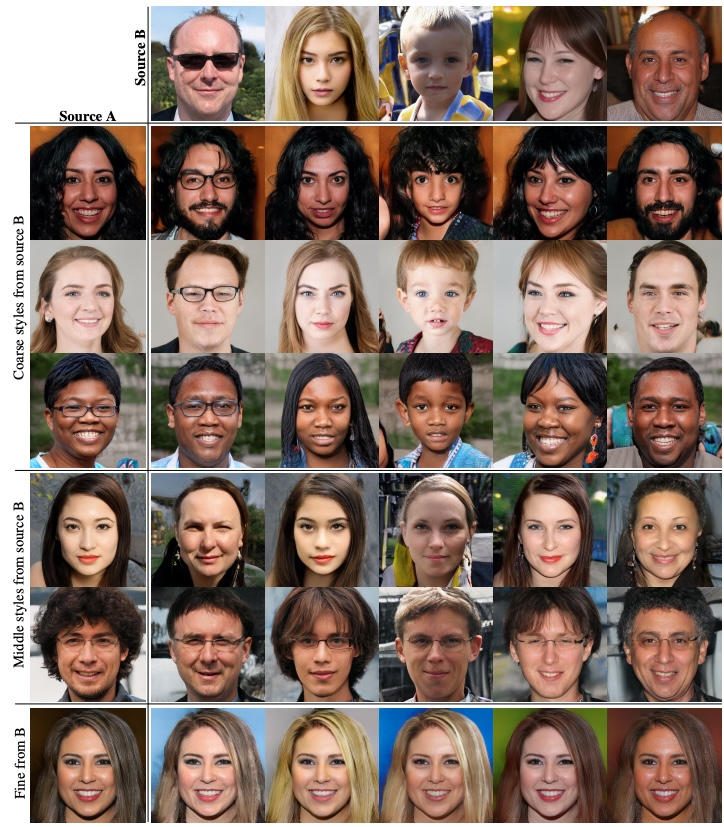
\includegraphics[width=0.7\linewidth]{images/related/stylegan_styles.jpg}
      \end{center}
      \caption{Synthesis control from latent space manipulation. Figure taken from \cite{karra2019stylegan}}
      \label{fig:stylegan_styles}
  \end{figure}

\subsubsection{Conditional GANs}
\ac{GAN}s can be conditioned on some condition $c$, known as \ac{cGAN}s \citep{mirza2014conditional}.
\ac{cGAN}s condition both the generator and discriminator on the condition, and Equation \ref{eq:gan_objective}
can be rewritten as follows:

\begin{equation}\label{eq:gan_objective}
      \min_{G}\max_{D}\mathbb{E}_{x, c\sim p(x, c)}[\log(D(x, c))] + \mathbb{E}_{z\sim p(z), c\sim p(c)}[\log(1 - D(G(z, c), c))]
\end{equation}

The condition can be a class label, a vector, or an image. The latter case is known as image-to-image translation,
and will be discussed in more detail in section \ref{subsection:image-to-image models}.
Although unconditional \ac{GAN}s achieved remarkable, photo-realistic synthesis on restricted datasets
like faces, conditional  \ac{GAN}s historically struggled on more diverse datasets like ImageNet. 
In 2019, however, significant progress on this front was made with BigGan \citep{brock2018large}, 
which achieved state-the-art results on ImageNet, significantly outperforming previous methods. They 
used a residual architecture, \ac{GAN} hinge loss \citep{lim2017geometric} (a variant of the adversarial loss),
 spectral normalization \citep{miyato2018spectral},
 class-conditional Batch Normalization \cite{ioffe2015batch}, scaling up the layer sizes, 
and increased
batch size. BigGAN remained state-of-the-art for
 ImageNet synthesis 
for several years until diffusion models outperformed them, which we describe in the
 next section. Class-conditioning helps provide the \ac{GAN} with additional information, helping training stability and mode-collapse.
 If, however, data labels are not available, unconditional \ac{GAN}s struggle to represent a diverse distribution like ImageNet.
 To combat this, \cite{casanova21nips} proposed Instance-GAN, where the generator and discriminator are 
 conditioned on a single SwAV~\citep(caron20nips) embedding of a real image. The discriminator then only observes the $K$ nearest-neighbors 
 as "real samples" while the generator aims at generating images close to the input image. Generating a variety 
 of samples is possible in this way even without labels.



\subsection{Denoising Diffusion Probabilistic Models}\label{sec:diffusion:models}

Although \ac{DDPM}s have roots dating from earlier years \citep{sohl2015deep}, the model became 
especially prominent in 2020 by \cite{ho2020denoising}, using a UNet architecture 
as the denoiser, which has since become standard practice. \cite{ho2020denoising} acheived 
similar results to their 
\ac{GAN} counterparts for various datasets. Then, \cite{dhariwal2021diffusion} adapted 
the model and achieved state of the art results on ImageNet and various LSUN datasets like 
Bedrooms, Horses and Cats, outperforming BigGAN \citep{brock2018large} and StyleGAN \citep{karra2020stylegan2}. 
Recently, \ac{DDPM}s achieved image synthesis from free-form text of remarkable quality \citep{ramesh2022hierarchical, nichol2021glide, saharia2022photorealistic, gafni2022make, rombach2022high}, 
These models capture complex intrinsic knowledge about the world from the billions of images used to train them \citep{schuhmann2022laion}, which 
allows high-quality generation of even completely imaginary concepts, like "a dragon fruit wearing karate belt in the snow."

In this section, we will first present the general framework of diffusion models. Then, we will 
present their conditional variant and techniques used to improve synthesis quality. Finally, 
we will go into more detail of some of the recent prominent models which have achieved photo-realistic 
results.

\subsection{Framework}

Introduced by \cite{sohl2015deep} and improved by \cite{ho2020denoising}, the \ac{DDPM} is a class 
of generative models trained to remove various levels of noise added to an input training image, as illustrated in Fig.\ref{fig:gen_models}.
Given an input image $\x_0$, the \emph{forward process} refers to the creation of the latent variables 
$\x_1, ..., \x_T$ by gradually noising the latents incrementally with gaussian noise, controlled by 
a variance schedule ${\beta_t}$ which grows from $0$ to $1$. Note that the schedule of 
$\beta_t$ is an implementation choice: \cite{ho2020denoising} proposed a linear schedule while 
\cite{dhariwal2021diffusion} proposed a cosine-based schedule which improved performance.

Concretely:

\begin{equation}
      \x_t = \sqrt{1 - \beta_t} \x_{t-1} +  \sqrt{\beta_t} \epsilon
\end{equation}

By posing $\alpha_t = \prod_{i=1}^{T} (1 - \beta_i)$ and through reparameterization, 
a nice property of \ac{DDPM}s is that we can always express a latent map $\x_t$ in relation 
to the initial image $\x_0$:

\begin{equation}
      \x_t = \sqrt{\alpha_t} \x_0 +  \sqrt{1 - \alpha_t} \epsilon
\end{equation}

Where $t$ varies from $0$ to $T$ and determines the mixing coefficient $\alpha_t$, which monotonically 
decreases from  $\alpha_0 = 1$ (no noise) to $\alpha_T \simeq 0$ (almost pure noise) for a large integer $T$.


The \emph{reverse process} refers to learning a model  $\epsilon_\theta$  which approximates the noise added at a given 
timestep $t$. Specifically, \ac{DDPM}s are trained with the following objective:

\begin{equation}
      \mathcal{L} = \displaystyle \mathbb{E}_{\x_0, t, \epsilon} \Vert \epsilon - \epsilon_\theta(\x_t, t) \Vert_2^2,
\end{equation}


% This training is performed for different values of the mixing coefficient $\alpha_t$, monotonically decreasing from $\alpha_0 = 1$ (no noise) to $\alpha_T \simeq 0$ (almost pure noise) for a large integer $T$.



% The level 
% of noise is determined by a timestep $t$, which varies from $0$ (no noise) to a large integer $T$ (pure gaussian noise).

% % Given a datapoint sampled from a real data distribution $\mathbf{x}_0 \sim \mathcal{D}_\mathcal{X}$, 


% \ac{DDPM}s \citep{ho2020denoising} is a class of generative models trained with the following image denoising objective:

% \begin{equation}
%     \mathcal{L} = \displaystyle \mathbb{E}_{\x_0, t, \epsilon} \Vert \epsilon - \epsilon_\theta(\x_t, t) \Vert_2^2,
% \end{equation}
% where $\epsilon_\theta$ is a noise estimator network trained to predict the noise $\epsilon \sim \gaussian$  an input image $\x_0$ in the following way: $\x_t = \sqrt{\alpha_t} \x_0 +  \sqrt{1 - \alpha_t} \epsilon$. This training is performed for different values of the mixing coefficient $\alpha_t$, monotonically decreasing from $\alpha_0 = 1$ (no noise) to $\alpha_T \simeq 0$ (almost pure noise) for a large integer $T$.

\minipar{Sampling}

At inference time, a new sample from the training distribution can be obtained by starting from 
random Gaussian noise $\mathbf{x}_T \sim \mathcal{N}(\mathbf{0}, \mathbf{I})$, and iteratively
refining it with the noise estimator network with the following equations, called 
\textit{DDPM sampling equations} \citep{ho2020denoising}:

\begin{align*}
      \hat{\x}_0 &= \frac{1}{\sqrt{\alpha_t}}(\x_t - \sqrt{1 - \alpha_t} \cdot \epsilon_\theta(\x_t, t)) \\
      \x_{t-1} &= \frac{(\alpha_{t-1}-\alpha_t) \sqrt{\alpha_{t-1}}}{\alpha_{t-1}(1 - \alpha_t)} \hat{\x}_0 + \frac{(1-\alpha_{t-1})\sqrt{\alpha_t}}{(1 - \alpha_t)\sqrt{\alpha_{t-1}}} \x_t + \sigma_t \z
\end{align*}

where $t$ goes from $T$ to $1$, 
$\sigma_t$ is a variance parameter (either learned or fixed), and $\z \sim \gaussian$.
In practice, the noise estimator network is modelled as a UNet \citep{ronneberger2015UNet} 
which inputs the noise map $\x_t$ concatenated with the timestep embedding of $t$. 


Without any modification, sampling with diffusion models is very costly, as it requires $T$
(which is usually on the magnitude of several thousands) forward passes to generate an image, a much slower 
process than their \ac{GAN} counterparts which only require one forward pass. On a modern 
GPU, a single sampling takes several minutes. \cite{nichol2021improved} shows that we can 
resample the number of steps and obtain their corresponding variances and perform fewer 
sampling steps during inference. They show that $100$  steps is sufficiant for high-quality 
generation with their model trained with $4000$ steps. \cite{song2021denoising} show that 
this strategy works even better with a deterministic model, and can reduce the amount of steps
down to $~20$. Finally, \cite{rombach2022high} show that we can considerably reduce training and 
inference complexity by working with latents $\x_t$ in a compressed space rather than 
the original image dimensions.

\subsection{Conditional DDPMs}\label{subsection:conditional_ddpm}

Conditional diffusion models \citep{chen2021wavegrad, saharia2022image, saharia2022palette}
make the denoising process conditional on a signal. Like other conditional generative models, 
this can be  a text, image, segmentation map, etc. In practice, the conditioning is 
typically done with concatenation to the noise map for modalities other than text, 
while text typically conditions the generation in multiple layers of the 
UNet through attention mechanisms \citep{nichol2021glide, rombach2022high, saharia2022photorealistic}.

\paragraph{Classifier-Guidance}
% dhariwal2021diffusion ADM
To improve generation quality, \cite{sohl2015deep, song2020score, dhariwal2021diffusion} show that 
it's possible to make use of an auxiliary classifier
during sampling to further guide the generation towards the desired output. 
In particular, an auxiliary classifier $p_\psi(y|\x_t, t)$ can be trained on images of varying noise 
$(\x_t, t)$ 
and be then used to guide the sampling during inference with its gradient 
 $\nabla_{\x_t} \log(y|\x_t, t) $ further towards the class $y$. 
 \cite{nichol2021glide} similarly shows improved results by using the CLIP \citep{radford2021learning}
 model as the classifier.
% ADM; look

\paragraph{Classifier-free Guidance}
% ho2022classifierfree
\cite{ho2022classifierfree} improves upon classifier guidance by 
proposing classifier-free guidance. Instead of using an auxiliary classifier, 
classifier-free guidance uses the \ac{DDPM} itself to further guide the 
generation. Concretely, it consists in tweaking the training of a conditional \ac{DDPM} 
by dropping the text or class label for a percentage of the time (usually, $20\%$)
and instead train with a null-text token or null-class label $\emptyset$. Then, during 
sampling, the output of $\epsilon_\theta$ is extrapolated further in the direction 
of the class or text with:

\begin{equation}
      \hat{\epsilon_\theta}(\x_t|y) = \epsilon_\theta(x_t, \emptyset) + s \cdot (\epsilon_\theta(x_t, y) - \epsilon(x_t, \emptyset))
\end{equation}

\noindent where $s > 1$

\cite{nichol2021glide} shows the superiority of this guidance compared to classifier-guidance,
and classifier-free guidance is currently standard practice for conditional diffusion models.

\subsection{Prominent Diffusion Models}

Initially, unconditional or class-conditional diffusion models were trained on small 
datasets which allowed benchmarking against \ac{GAN}s \cite{ho2020denoising, dhariwal2021diffusion}.
Recently, works started to train diffusion models on very large billion-element text-image 
datasets \citep{schuhmann2022laion} which allowed unprecedented generation  in terms of 
photorealism and diversity. GLIDE \citep{nichol2021glide} built off the architecture in 
\cite{dhariwal2021diffusion} to adapt class-conditioning to text-conditioning. DALL-E 2 \citep{ramesh2022hierarchical}
also built on this architecture, but conditioned the generation on  CLIP \cite{radford2021learning}
encodings of the image to "unCLIP" the embedding. Imagen \citep{saharia2022photorealistic} a leveraged 
a much larger language model for the text encoder which conditioned generation, showing that 
performance scales with the text encoder size but not with the UNet size. Latent Diffusion Models \citep{rombach2022high}
first compresses images into a $~8\times$ reduced space with an encoder before performing the 
diffusion process on these latents, rather than the noised images. Their model requires much 
less ressources for training and also allows for a much faster inference speed. Other models, 
like MidJourney


\section{Image Editing}\label{section:image_editing}

Image editing is a particular case of image synthesis which requires (1) a way to use the 
input image as input and (2) a specific editing task. There are two ways to approach this 
problem: training/fine-tuning a network for the task (\ref{subsection:image-to-image models}) or 
leveraging a pre-trained network, which has already learned powerful semantics, and tweaking the 
internal feature-maps or latent code (\ref{subsection:hacking_generative_model}, \ref{subsection:latent_space_manipulation}).
We can look at these approaches from a "coarse-to-fine" point of view - image-to-image models (\ref{subsection:image-to-image models})
typically train an entire network from scratch to perform the task at hand, "hacking" generative models (\ref{subsection:hacking_generative_model})
manipulate a subset of internal feature-maps or weights from a pre-trained network, and latent space manipulation (\ref{subsection:latent_space_manipulation})
leave the entire network as is, only manipulating the latent code input. The approaches typically 
vary on the "controllability - practicality" tradeoff. That is, the less we manipulate a pre-trained 
network, the more tied we are to the original dataset the network was trained on. However, re-training 
a new network as is typical in image-to-image models requires much more data (which we may not have)
and training resources. For the "average" person, it is infeasible to train a model as semantically powerful as 
state-of-the-art generative models (Stable Diffusion \citep{rombach2022high}, for example, cost $\$160,000$ and 
$80,000$ A100 \citep{gpua100} hours to train \citep{MosaicML}). Moreover, state-of-the-art generative models 
intrinsically learn powerful concepts, which can be leveraged (see \ref{subsection:latent_space_manipulation}). 
To summarize, all the following approaches have their merits, and as a general "guideline", the more the 
input image deviates from the domain of a pre-trained model, the more tweaking (or new training) a user 
should do.

\subsection{Image-to-Image Models}\label{subsection:image-to-image models}
Image-to-image models can be seen as a straightforward way to perform image editing when 
we wish to "translate" an image from a source domain $A$ to a target domain $B$. In this case, the entire image is typically 
edited to (1) keep prominent structures of the source image and (2) belong to the target 
domain. Typical application of these include sketches to photos, photos to paintings, 
semantic maps to photos, colorization, etc. The task of inpainting, which consists in generating a missing 
part of an input image, is a particular case of image-to-image models and will be discussed in depth in 
Chapter \ref{chapter:gradpaint}. Image-to-image translation has almost exclusively been worked on using \ac{GAN}s except 
in recent works which 
adapted \ac{DDPM}s for the task. In the case where we have access to paired data  containing 
before and after images, \cite{pix2pix} proposed a general framework "Pix2Pix" using a \ac{cGAN} 
where both the generater and discriminator are conditioned by the input image as well as a fully-convolutional 
discriminator "PatchGAN", which discriminates patches as real or fake and then aggregates the results.
The authors 
proposed a UNet architecture with skip connections since the input and output images generally share 
many similar edges and features. The work used an $L1$ loss as well as a \ac{GAN} loss,  
encapsulating the two objectives stated above. Pix2PixHD \citep{wang2018pix2pixHD}
extended this framework for 
high-resolution images ($2048 \times 1024$). Pix2PixHD used a similar idea to Progressive Growing (see 
section \ref{par:progressive_growing}) and first trains a low-resolution generator before  
adding a high-resolution generator to the architecture, with both architectures remaining fully-trainable.
Multi-scale discriminators were also added for further training stability.
Later  \ac{GAN}-based works extended this, first with spatially-adaptive normalization layers \citep{gaugan} and then
later with a more powerful, spatially-aware discriminator which eliminates the need for a reconstruction loss \citep{sushko2020you}.
 More recently, \cite{psp} adapted the image-to-image framework by training 
an encoder-decoder network in which the encoder predicts latent codes of StyleGAN2 \citep{karra2020stylegan2}
to reconstruct the image. With restricted domains where StyleGAN2 excels, such as faces, this produces  
very natural results, unlike the Pix2Pix (and successors) frameworks, which are prone to artifacts.
Recently, conditional \ac{DDPM}s aborded the image-to-image translation tasks, such as super-resolution \citep{saharia2022image} and 
inpainting \citep{nichol2021glide}. \cite{saharia2022palette} provide a general image-to-image framework with \ac{DDPM}s, 
which builds upon the architecture from \cite{dhariwal2021diffusion} and concatenating the source image with 
the noise map at every denoising step, as described in \ref{subsection:conditional_ddpm}. 

In the case where we don't have access to paired data, different approaches exist. 
A straightforward approach consists in solely performing style transfer \citep{huang2017arbitrary}
for adapted cases, like photos to paintings. They use a fixed pre-trained VGG encoder \citep{simonyan2014very}
and a trainable decoder network which is trained with a content loss and a style loss (calculated by using 
the same VGG network). \cite{cyclegan} produced a novel approach, CycleGAN, which consists in training two \ac{GAN}s, 
along with a cyclic loss the translated source image translated back to the source domain should produce the 
initial source image.  \cite{choi2018stargan} and later \cite{choi2020stargan}
proposed a general framework for unsupervised image-to-image translation in the case of multiple domains. The works 
noted that generalizing a CycleGAN approach  would result in a quadratic amount of \ac{GAN}s to train.
Instead, \cite{choi2020stargan} trains one \ac{GAN}, in which the discriminator predicts scores for each domain, 
one style encoder, which outputs a style given an image, and one mapping function, which outputs a style given 
a source domain and a latent vector. The work conditions the generator with the style encoding
and allows realistic translations for multiple domains. Recent works with \ac{DDPM}s leveraged large and powerful 
pre-trained models for down-stream image-to-image translation tasks, requiring as little as 1000 labelled 
training data to perform high-quality image-to-image translation \citep{zhang2023adding, wang2022pretraining, voynov2022sketch}.

\subsection{"Hacking" a generative model}\label{subsection:hacking_generative_model}
We refer to "hacking" a generative model as manipulating the network's internal trained weights 
or feature maps in order to have fine-grained control of the output generation. These methods 
have roots in understanding how the internal structure of \ac{DNN}s affect their prediction \citep{collins2018deep, zeiler2014visualizing, strobelt2017lstmvis, karpathy2015visualizing, chen2019delving}.
\cite{bau2018gan} extended this to \ac{GAN}s, and showed that specific feature maps in a pretrained \ac{GAN}
corresponded to different concepts. After finding the specific feature maps, they showed that setting 
the feature map values to 0 or to a given constant respectfully ablated or generated the concept 
in question. \cite{bau2020semantic} showed in a later work that this can be extended to real images 
with inverting a real image into the \ac{GAN} latent space. \cite{editing_style} extends this work 
by using spherical k-means to pick out fine-grained concepts before finding their corresponding feature maps 
to manipulate. They work with the StyleGAN2 latent code, which (being more disentangled) produces more 
aesthetically pleasing results. \cite{stylespace_analysis} does similar work, except only using the 
style code (the code after the affine transformations of the latent code) for manipulation. \cite{bau2020rewriting} 
showed that it's possible 
to "rewrite" a generative model to produce images based on user-given images, such as mustaches which 
replace eyebrows. They showed that by re-optimizing a small subset of weights for the output to match 
the user-generated output, the new rules of the generative model generalize for new images. 
\cite{cherepkov2021navigating} shows that it's possible to discover possible edits in the parameter
space of a StyleGAN.
Finally, 
\cite{hertz2022prompt} "hijacks" a pre-trained \ac{DDPM} by manipulating the cross-attention maps 
(between pixels and text tokens). They generate a first image with a source text, another image 
with a target text, and then copy/paste values from the cross-attention maps of the latter case into 
the former case, which edits the first image with the target text. 

\subsection{Latent Space Manipulation}\label{subsection:latent_space_manipulation}
Latent space manipulation can be seen as a particular case of the previous section where the manipulation 
is completely limited to the latent space (i.e. the input to the very first layer of a classic \ac{GAN}
like \ac{DCGAN} or the latent code which gives the style code for style-based \ac{GAN}s). 
Early work on \ac{GAN}s \citep{dcgan} showed that by performing arithmetic in the pre-trained 
\ac{GAN}'s latent space, we are able to control the generation. For example, they showed that
if they obtain latent vectors $a$, $b$ and $c$ respectfully for "a man with glasses", 
"a man without glasses", and "a woman without glasses", performing $a - b + c$ gives a latent 
vector which produces images of a woman with glasses. Works in latent space manipulation
 particularly boomed with the arrival of StyleGAN \citep{karra2019stylegan}
and StyleGAN2 \citep{karra2020stylegan2} with their powerful semantic, localized and 
disentangled latent space. \cite{harkonen2020ganspace} showed that performing PCA in the 
latent space of 
a \ac{GAN} allows localization and edition of high-level concepts, like gender for faces or 
color for cars. Similarly,
\cite{voynov20icml} shows that we can discover important directions in the latent space by 
training a network to predict the shift that was used in the latent code to produce two generated images. 
\cite{shen2020} and \cite{zhuang2021enjoy} use auxiliary networks 
which predict image attributes and learn the mapping between latent vectors and image features.
\cite{Goetschalckxganalyze} also uses an auxiliar network which predicts the aesthetics of an 
image. They train a simple network which learns to modify the latent code of BigGAN \citep{brock2018large}
such that the resulting image is either less or more memorable.
 \cite{zhang2021datasetgan}
shows that by manually semantically segmenting a few images, we can learn how to automatically 
segment newly generated images just from their latent code, thus creating a dataset "for free".
 \cite{ling2021editgan} then leverages this work to edit 
the images by modifying the corresponding segmentation map, and then finding the corresponding latent code to regenerate 
the edited image. \cite{tewari2020stylerig} and \cite{zhang2020image} show that StyleGAN2's latent code 
learns 3D information which can be leveraged to perform 3D edits of the input image.

 Although 
these works typically focus on \ac{GAN}s, \cite{khrulkov2022understanding} shows that the latent code of 
\ac{DDPM}s is also of interest - using the same latent code for totally different 
\ac{DDPM}s produce similar images in terms of semantics and colors, showing that \ac{DDPM}s generate 
images from the latent code through optimal transport.

% \subsection{Conditional Generative Models}
% Conditioning on stuff.

% \subsection{"Hacking" a generative model}
% --> talk about gan based (what i presented in the very beginning), then best paper one time where 
% they were able to draw mustaches on faces. 
% Then diffusion based models.

% - historically; GAN-based 
% - talk about pix2pix
% - spade 
% - latent manipulation methods
% - optimizing "adversarial examples" in latent space - talk about later. 
% - editing w/ diffusion models 



\section{Evaluation for image synthesis and editing}

\subsection{Evaluation Metrics}

The models described above provide ways to sample new generated images from the learned model. 
Measuring image quality, however, is not straightforward like classification tasks. Indeed, when 
classification accuracy can simply be evaluated with a validation test using the trained model, 
image quality requires us to compare two distributions to each other, the real images and the 
generated images. When evaluating models for the task of image synthesis, we have two goals in mind:
fidelity and diversity. Fidelity refers to the quality of generated samples in relation to the 
source dataset. Diversity refers to the variety of images in relation to the source 
dataset.


\minipar{Inception Score}
The \ac{IS} was introduced by \cite{improved_techniques_gans} as a way to evaluate 
\ac{GAN}s for diversity and fidelity. \ac{IS} relies on a pre-trained classifier 
(typically a pre-trained InceptionV3 model \citep{szegedy2016rethinking}) which classifies the 
generated samples $x$ to ImageNet classes $y$. \ac{IS} calculates the \ac{KL}-Divergence $(p(y|x) || p(y))$ between the 
conditional distribution $p(y|x)$  and the marginal distribution $p(y)$.
The intuition 
is that the conditional distribution $p(y|x)$ should have low-entropy (high probabilities 
imply high image-quality)
and the marginal distribution $p(y)$ should have high-entropy (equal probabilites 
among classes implies diversity). In this case, 
a high \ac{IS} means better performance. This score has notable drawbacks - 
primarily that there there does not have to be any diversity within a generated class 
to obtain a perfect score. Secondly, there is no comparison to the distribution of 
real dataset. Finally, this score specifically tailers to ImageNet classes, and 
makes less sense to evaluate on specific domains like human faces or bedrooms. This metric
 is typically not used anymore.

\minipar{FID}\label{sec:related_fid}


The \ac{FID} score \citep{heusel2017gans} was proposed to adress these drawbacks and 
was found to be more consistent with human evaluation. This score uses a pre-trained 
classifier (again, typically the Inception V3 network) as a feature-extractor for the 
real and the generated images.  \ac{FID}
fits a multivariate normal distribution to the generated and real extracted features and 
computes the Fréchet Distance between these statistics, which can be computed in closed-form.
In this case, a small value is better as it signals similarity between the real and generated 
distributions. \ac{FID} is very sensitive to different implementations and different sample sizes. 
The higher the sample size, the more reliable \ac{FID}, and it requires a sample size of at least 
the size of the InceptionV3 feature space ($2048$) for a somewhat accurate estimate. 
For datasets smaller than this minimum size, the \textbf{\ac{SFID}} was proposed 
\citep{kim2020simplified}, which does
 not take into account the offdiagonal terms in the feature covariance matrix
 to avoid numerical instability. 
 More formally, let $\mu^r$ and $\sigma^r$ be the mean and standard deviation of 
inception features for the real images, and $\mu^s$ and $\sigma^s$ for the synthetic 
images. The \ac{SFID} \cite{kim2020simplified} is computed as 


\begin{equation}
      SFID(\alpha) = \lVert \mu^r - \mu^s \rVert ^2 + \alpha \lVert\sigma^r - \sigma^s\rVert^2.
      \end{equation}
 
 Finally, the \ac{CFID} (respectfully, \ac{CSFID}) is computed in the same manner as the \ac{FID}
 (respectfully, \ac{SFID}) but for each target class separately, and then averaging the resulting scores.

 Specifically, with $\mu^r_c$ and $\sigma^r_c$ the mean and standard deviation of inception 
 features for the real images belonging to class $c$, and $\mu^s_c$ and $\sigma^s_c$ 
 for the synthetic images, we have
\begin{equation}
CSFID(\alpha) = \frac{1}{|C|} \sum_c \lVert \mu^r_c - \mu^s_c \rVert ^2 + \frac{\alpha}{|C|} \sum_c \lVert\sigma^r_c - \sigma^s_c\rVert^2.
\label{eq:sfid}
\end{equation}
where $\alpha$ is a parameter to choose. 
 
 


\ac{FID} and its variants
still face the drawbacks of using an ImageNet pre-trained classifier for performance, which 
 makes less sense for restricted domains like faces or very large datasets like LAION-5B \citep{schuhmann2022laion}, 
 although this can be circumvented by using 
a domain-specific pre-trained classifier. In this case, results between papers are not easily 
comparable and re-calculation is necessary~\citep{dhariwal2021diffusion}. 

\minipar{Precision and Recall}  The Precision and Recall metrics were proposed by~\cite{sajjadi2018assessing} and 
later improved by~\cite{kynkaanniemi2019improved}. Let's consider the two manifolds of real images $P_r$ and 
generated images $P_g$.
Precision, similar to Fidelity, refers to the chance that a generated image looks real (falls within $P_r$) while 
Recall, similar to Diversity, refers to the chances that a real image can be generated (falls within $P_g$).
See~\ref{fig:precision_recall} for a visualization. While the \ac{FID} score aimed to fit a statistical model 
to define these two distributions $P_g$ and $P_r$, Precision and Recall estimates these distributions 
using a nearest-neighbor approach. Specifically for a set of $N$ real images
and $N$ generated images, we first extract their features with a pretrained
feature extractor $f$ and obtain their respective manifolds $\Phi_r$ and $\Phi_g$. 
Then, a given extracted feature $\phi = f(x)$ belongs to manifold $\Phi$ if $h(\phi, \Phi) = 1$, where 

\[
      h(\phi, \Phi) = 
\begin{cases}
    1,& \text{if } \exists f(\phi') \in \Phi \text{ such that }||\phi - \phi'||_2 \le ||\phi' - NN_k(\phi', \Phi)||\\
    0,              & \text{else}
\end{cases}
\]

\noindent where $k$ is a parameter to define and $NN_k(\phi', \Phi)$ is the $k^{th}$ nearest neighbor of $\phi'$ in $\Phi$.

Finally, precision can be defined as:

\begin{equation}
      \text{precision}(\Phi_r, \Phi_g) = \frac{1}{|\Phi_g|}\sum_{\phi_g \in \Phi_g}{h(\phi_g, \Phi_r)}
\end{equation}

And recall as: 
\begin{equation}
      \text{recall}(\Phi_r, \Phi_g) = \frac{1}{|\Phi_r|}\sum_{\phi_r \in \Phi_r}{h(\phi_r, \Phi_g)}
\end{equation}


Precision and Recall was shown to correlate with human perception and allows us to 
diagnose synthesis problems more precicesly (\ac{FID} encapulates both diversity and fidelity 
in one single metric which sometimes doesn't allow granularity). Moreover, with this nearest-neighbor 
approach, we can say that an image is \emph{realistic} if there exists a feature vector in $\Phi_r$
which is closer to the test image's feature vector than to its $k^{th}$ nearest neighbor.

% \begin{equation}
%       \text{realism}(\phi) = \max_{\phi_r}{\frac{||\phi_r - NN_k() ||}{||\phi - \phi_r||}}
% \end{equation}


\begin{figure}[tb]
      \begin{center}
          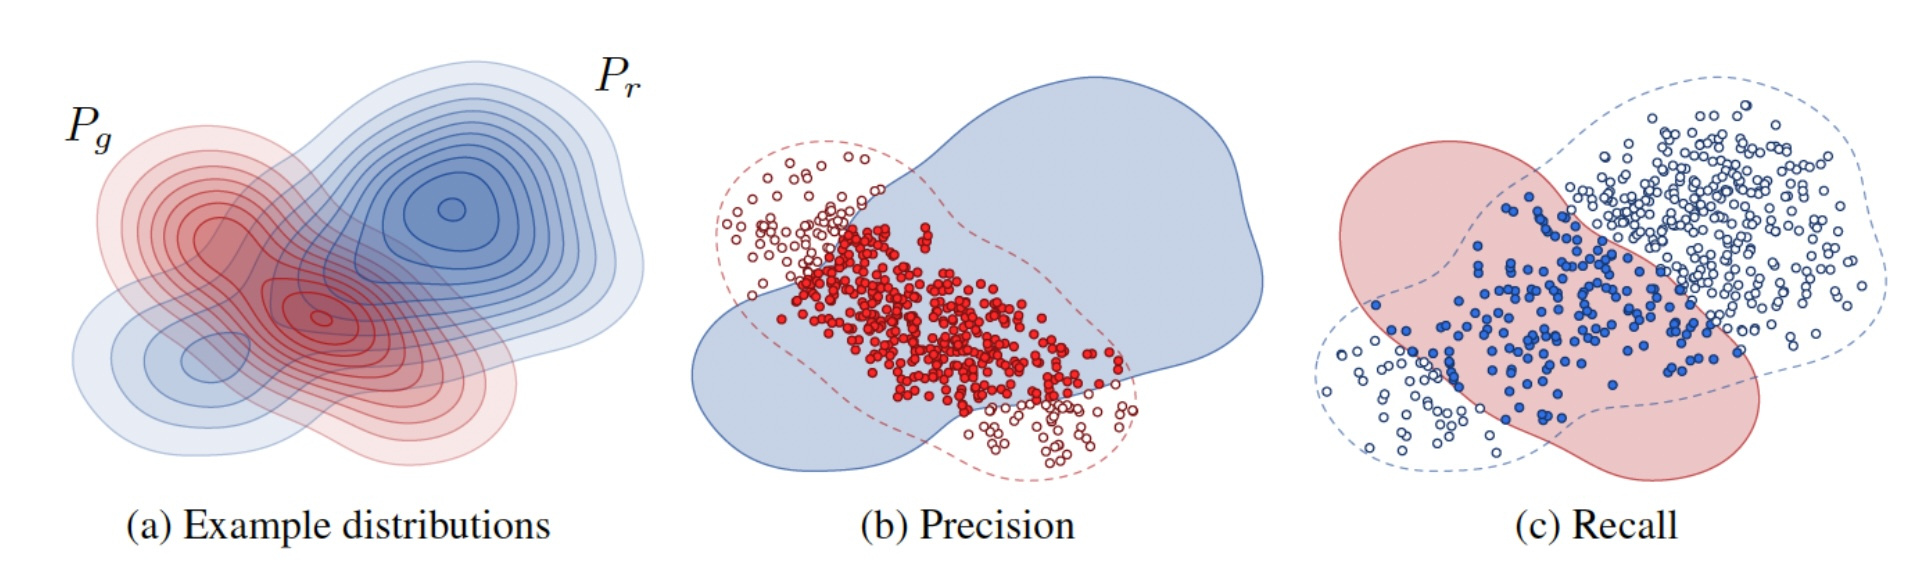
\includegraphics[width=0.7\linewidth]{images/related/precision_recall.jpg}
      \end{center}
      \caption{Precision and Recall. (a) shows the real  distribution $P_r$ and generated distribution $P_g$. (b) Precision: How likely that an image from $P_g$ falls within $P_r$? (c) Recall: How likely that an image from $P_r$ falls within $P_g$? Figure taken from \cite{kynkaanniemi2019improved}}
      \label{fig:precision_recall}
  \end{figure}


However, there are problems associated with these Precision and Recall metrics \citep{naeem2020reliable, alaa2022faithful}.
Notably, they are not robust to outliars in the generative and real datasets. Note that a generative model which only barely 
covers dense modes of the real dataset and overwhelmingly 
produces samples resembling a few real outliars will have perfect precision and recall scores. To adress these, 
\cite{alaa2022faithful} recently proposed $\alpha$-Precision and $\beta$-Recall. $\alpha$-Precision is the 
fraction of generated examples which resemble the "most typical" fraction $\alpha$ of real samples, while  $\beta$-Recall
is the fraction of real samples covered by the most typical fraction $\beta$ of synthetic samples. By varying 
$\alpha$ and $\beta$ from 0 to 1, we can observe the effects of outliars and thus better evaluate the closeness 
of the real and generated distributions. 

\minipar{Authenticity} All of the above metrics are susceptible to a generative model simply "copying and pasting" 
the training data. Also proposed by \cite{alaa2022faithful}, authenticity refers to the rate at which 
a model generates new samples. With  $\alpha$-Precision, $\beta$-Recall and authenticity, \cite{alaa2022faithful}
shows that we can more reliably evaluate generative models compared to existing approaches. 

\minipar{CLIP similarity} \ac{CLIP}~\cite{radford2021learning} introduced a text and image encoder trained 
jointly on 400M web-crawled image/text pairs 
with a simple contrastive InfoNCE loss \citep{oord18arxiv}. In the case of text-guided image editing, 
the \ac{CLIP} similarity score measures the distance in the embedded space 
between the target textual description and the edited image.  This score is especially used in recent 
works which perform highly flexible editing \citep{mokady2023null, hertz2022prompt}.

\minipar{LPIPS}\label{sec:related_lpips}
In the case of image editing, we can measure the LPIPS \citep{zhanglpips2018} score between 
the real image and the edited image. It is a weighted $\ell_2$ distance of deep image features, 
where the weights have been learned to be able to predict human perceptual similarity  between patches.
This metric was shown to correlate well with human perceptual similarity, unlike other full-reference metrics
 (like the $\ell_2$ distance between pixels). While editing should change the image slightly, an 
edited image should generally not deviate profoundly from the input image. This metric 
is generally used alongside  other metrics which measure image quality. 

\minipar{Human Evaluation} 
Human evaluation remains a main way of evaluating image quality.  \cite{hype} 
established a standard human benchmark for image evaluation, while other works propose 
more task-specific surveys. \ac{MTurk} remains a popular tool for image editing 
evaluation which allows a diverse pool of humans to choose their preferable 
image edit. 


\subsection{Datasets}

As image editing was historically limited to \ac{GAN}s, datasets used 
for evaluation typically used restricted datasets which could be covered by 
a \ac{GAN}'s domain. Typically, this meant either a validation set of the training 
set, or a different dataset altogether which is similar to the training set.

The most common of these restricted datasets are face datasets, since faces are 
of particular practical use for the public and they present regular structures which 
react better to generation and editing. Common face datasets
include

\begin{itemize}
      \item \textbf{CelebA} \citep{celeba}. It contains 200000 images of celebrity faces of medium-resolution (mostly $178\times218$). Each image is labelled with 40 different binary attributes (e.g. glasses, smile, etc.)
      \item \textbf{CelebAHQ} \citep{karras2018progressive}. A high-resolution extension of the previous dataset, containing 30000 images of $1024\times1024$ resolution.
      \item \textbf{FFHQ} \citep{karra2019stylegan}. Contains 70000 images of $1024\times1024$ resolution scraped from Flikr. This dataset was created to include a much larger variety of faces compared to the previous datasets (which only included celebrities), and includes a variety of ethnicities, genders, ages, and expressions.
\end{itemize} 

Other popular choices for evaluation  include:

\begin{itemize}
      \item Individual subdatasets from \textbf{LSUN} \citep{lsun}. LSUN bedrooms, LSUN Churches, LSUN cars, LSUN horses are popular choices. Each subset dataset contains about 1M images of varying resolution. 
      \item \textbf{Places2} \citep{zhou2017places}, especially a popular choice for training and evaluating inpainting tasks. It contains 10 million labeled images, covering a wide variety of indoor and outdoor scenes. The images are generally of high-resolution.
      \item \textbf{ImageNet} \citep{russakovsky2015imagenet_ilsvrc} about 1.2M images divided into 1000 classes. This dataset can be used for class-based editing.
      \item \textbf{COCO} dataset \citep{caesar2018cocoostuff} for text-based editing. This contains 330000 images, each annotated with 5 captions. 
\end{itemize}

It is worth noting that the recent open-source large-scale diffusion model Stable-Diffusion was trained 
on the public dataset \textbf{LAION-5B} \citep{schuhmann2022laion}. This dataset contains 
5 billion image-text pairs scraped off the web. Text-guided editing methods which use Stable-Diffusion, 
in addition to evaluating on the above datasets, often evaluate on custom-made datasets \citep{bar2022text2live, mokady2023null} of more diverse nature which contain a variety of object categories and 
text prompts for editing.


\section{Our contributions and positioning}

We abord the task of image editing with three different approaches, constituating our three 
contributions. We will present these contributions in the three following chapters, which 
are summarized below.

\paragraph{Chapter 3: Real-Image Editing with a pre-trained \ac{GAN}}

Firstly, we wanted to leverage the existing works on latent-space manipulation for a pre-trained \ac{GAN} 
(\ref{subsection:latent_space_manipulation}). We remarked that existing works performed powerful and 
convincing edits for generated images, but generalized poorly to real images. In order to apply the 
aformentioned techniques to real images, we must first invert the real image into the pre-trained \ac{GAN}
to obtain its corresponding latent code (since \ac{GAN} have no inherent encoder network). Motivated by 
the success of works on latent-space manipulation, we show that we can use a similar technique to 
perform the inversion of a real image, and thus obtain an editable latent code. We extensively 
quantitatively and qualitativly evaluate our method on faces and cars datasets.

\paragraph{Chapter 4: Flexible text-guided image editing}

Although our first contribution works well for images within a pre-trained \ac{GAN}'s  domain, 
editing a more complicated image works poorly. For our second work, FlexIt, we thus took advantage of the 
recently proposed  VQGAN \citep{esser2021taming} (a type of \ac{VAE}) to directly encode images into a codebook of vector-quantized
feature vectors. We optimize this latent space to match the user's target text using the recently proposed 
CLIP dual-encoder \citep{radford2021learning}. Because the \ac{VAE} was not trained to generate images,
its latent code does not capture semantic information like a \ac{GAN} does, and we thus introduce
 a way to efficiently tune our hyper-parameters 
 which encompasses our two 
objectives - (1) obtaining an edited image which matches the target text and (2) minimally changing 
the input image. We thorougly evaluate our method on the ImageNet dataset, showing that with cleverly
tuning of the hyper-parameters, we achieve better results than previous text-guided editing methods.


\paragraph{Chapter 5: Gradient-guided inpainting with a \ac{DDPM}}

We again examined the short-comings of our previous works. While FlexIt can indeed edit any image, 
the \ac{VAE}'s encoder inherently loses original details present in the source image. Moreover,
the lack of generative knowledge within the model can sometimes lead to absurd edits which 
we cannot control. For real-life 
use-cases, this is not permissible. An editing task can be seen as a conditional inpainting 
task, in which the condition only holds effect in the region defined by the inpainting mask. We thus 
aborded the question of inpainting with \ac{DDPM}s. Because of their gradual inference nature, we can 
guarantee zero image fidelity loss in the regions outside of the inpainting mask while continually 
blending the generated output with the known regions through noising and denoising. However, the 
denoising process is too fast for the blending to be successfully harmonized, inspiring works which 
forecfully slow-down the denoising process for better harmonization \citep{lugmayr2022repaint}. We 
go through a different route, and instead guide the denoising process with a gradient of a loss 
specific for harmonization between the two regions. Our method can be applied to unconditional \ac{DDPM}s 
as well as conditional ones, and we performed thorough evaluation on face datasets (CelebaHQ and FFHQ),
 ImageNet, COCO, 
and Places2. 



















% In this chapter, we detail the related work needed to read this thesis. We first briefly
% explain the learning procedure in \acf{DL} and how the data are structured. Then, we describe the main
% \ac{DL} applications and architectures in \acf{CV}. Finally, we introduce the main topic of this thesis
% ---Continual Learning--- and showcase the challenges, benchmarks, and methods of this domain. The
% notations introduced in this chapter and through the thesis are listed in the
% \hyperref[chap:notations]{Notations} section.

% \section{Neural Network Learning}

% Neural Networks are based on the statistical learning theory \citep{vapnik1999statstheory}. In the
% \textit{supervised setting}, the goal of a neural network is to learn the best mapping function $f :
%       \mathcal{X} \rightarrow \mathcal{Y}$ between an input space $\mathcal{X}$ and an output space
% $\mathcal{Y}$.  We consider a \textit{loss} function $\mcL : \mathcal{Y} \times \mathcal{Y}
%       \rightarrow \mathbb{R}^+$ that measures the disagreement between a ground-truth label $y$ and the
% network's prediction $\hat{\vy} = f(\vx)$. In the context of image classification, $\vx$ is the
% image pixels, $y$ is the \textit{class} label of the object present in the image, and $\hat{\vy}$ is
% a vector of probabilities, with one probability per class the model has to predict. The class with
% the highest predicted probability/confidence is chosen as the prediction. Given a \textit{training
%       dataset} $\mathbb{D} = \{(\vx_1, y_1), ..., (\vx_N, y_N)\}$, training a neural network consists in
% finding the set of parameters $\theta_*$ which minimizes the loss function:
% %
% \begin{equation}
%       \theta_* = \operatorname{argmin}_{\theta} \left \{ \frac{1}{|\mathbb{D}|}\sum_{(\vx,y)\in \mathbb{D}} \mcL(f_\theta(\vx), y)\right \}\,.
%       \label{eq:intro_optim}
% \end{equation}
% %
% However, the optimal set of parameters $\theta_*$ minimizing the loss on the training set, can fail
% to predict the correct label on the testing set. Therefore, to avoid this \textit{overfitting}
% phenomenon, regularization functions that limit the parameters space are used as additional
% constraints in addition to the classification loss $\mcL$.

% In practice, the function $f_\theta$ learned by a neural network is composed of a succession of
% linear transformations and non-linear \textit{activation} functions. For example, a simple neural
% network, called \ac{MLP}, here with two layers, could be defined as:
% %
% \begin{equation}
%       \hat{\vy} = f_\theta(\vx) = \operatorname{softmax}(\vW_o \sigma(\vW_h \vx + \vb_h) + \vb_o))\,,
%       \label{eq:intro_mlp}
% \end{equation}
% %
% \noindent with $\vW_h \in \mathbb{R}^{H \times D}$, $\vb_h \in \mathbb{R}^{H}$, $\vW_o \in
%       \mathbb{R}^{C \times H}$, $\vb_o \in \mathbb{R}^{C}$ being the parameters $\theta$ of the
% network. $\sigma$ is a hidden non-linear activation, often a \ac{ReLU}
% ($\operatorname{ReLU(x)} = \text{max}(0, x)$), and $\hat{y} = \operatorname{softmax}(\tilde{\vy}) =
%       \nicefrac{e^{\tilde{\vy}}}{\sum_{i} e^{\tilde{\vy}_i}}$ is the final non-linear activation.

% Likewise, in practice for image classification, the loss is often the categorical cross-entropy:
% %
% \begin{equation}
%       \mcL(\hat{\vy}, \vy) = -\sum_c y_c \log \hat{y}_c\,,
%       \label{eq:intro_ce}
% \end{equation}
% %
% \noindent with $\vy$ a one-hot vector of the labels. Finally, to optimize the parameters of the neural
% network (such as \autoref{eq:intro_optim}), we often use the mini-batch \ac{SGD} algorithm or a variation thereof:

% \begin{algorithm}
%       \begin{algorithmic}[1]
%             \Statex \textbf{input:} a dataset $\mathbb{D}$ with pairs of $(\vx_i, \vy_i)$
%             \Statex \textbf{input:} a loss function $\mcL$
%             \Statex \textbf{input:} a model function $f_\theta$ with $\theta$ the learned parameters
%             \Statex \textbf{input:} a learning rate $\eta$ and a batch size $b$
%             \Statex

%             \While{stopping criterion not satisfied}
%             \State $(\vx, \vy)$ $\gets$ sample mini-batch of size $b$ from $\mathbb{D}$
%             \State Forward pass: $\hat{\vy}$ $\gets$ $f_\theta(\vx)$
%             \State Compute loss: $\mcL$ $\gets$ $\mcL(\hat{\vy}, \vy)$
%             \State Compute the gradients: $\delta$ $\gets$ $\nabla_\theta \mcL$
%             \State Update all parameters: $\theta$ $\gets$ $\theta - \eta \delta$
%             \EndWhile
%       \end{algorithmic}
%       \caption{Procedure to optimize a neural network with gradient descent.}
%       \label{algo:intro_sgd}
% \end{algorithm}

% The learning rate $\eta$ controls the step size when updating the parameters in the direction of the
% gradient. The batch size $b$ defines the number of images seen during one update. The
% \textit{backpropagation} algorithm \citep{rumelhart1986backprop} computes the gradients and the
% update of the parameters. In the case of image classification and segmentation, the main topics
% explored in this thesis, we discern the \textit{feature extractor} from the \textit{classifier} in
% the neural network. The former transforms the input space so that the latter linearly discriminates
% classes. From now on, the feature extractor will be denoted by $f$, and the classifier by $g$ (see
% the \hyperref[chap:notations]{notations}). The model is then $g \circ f$.

% The neural network in \autoref{eq:intro_mlp} can be defined as \textit{shallow} with only one hidden
% layer. By extension, an important success of later neural networks came with training \textit{deep}
% neural network with multiple hidden layers. More generally in this thesis, we will refer to them as
% \acf{DL} models. The majority of \ac{DL} models, in \acf{CV}, in \acf{NLP}, or even in Audio are
% based on the same structure (linear transformations and non-linear activations) and are trained with
% a form of gradient descent.

% \section{Deep Architectures for Computer Vision}
% \label{sec:related_cv}

% A common type of architectures for computer vision is the \acf{ConvNet}. First defined by
% \citet{fukushima1980neocognitron} and then trained with backpropagation by \citet{lecun1999lenet},
% it is a neural network architecture whose linear operators are \textit{convolutions}. While
% handcrafted convolutions \citep{lowe1999sift} rely on well-defined features, a \ac{ConvNet} learns
% the convolution kernels to detect more complex patterns required to minimize the classification
% loss. In 2012, thanks to a large dataset and more efficient code working on \acp{GPU} allowing
% training larger networks, \citet{krizhevsky2012alexnet} won the ILSVC competition
% \citep{russakovsky2015imagenet_ilsvrc} where they had to classify a large dataset ---ImageNet---
% made of 1.28M training images and 1000 classes. From that point forward, multiple improvements were
% made to \acp{ConvNet} \citep{ioffe2015batchnorm,he2016resnet} and these methods have been applied
% not only to classification but also object detection \citep{ren20fasterrcnn}, semantic segmentation
% \citep{chen2018deeplab}, visual question answering \citep{antol2015vqa,benyounes2017mutan}, image
% generation \citep{goodfellow2014gan}, image editing \citep{grechka2021magecally,couairon2022flexit},
% \etc.

% Most \acp{ConvNet} follow a similar structure with blocks of convolutions and pooling. Often, the
% final spatial features are flattened by \ac{GAP} and fed to a linear classifier
% predicting the classes probabilities. \autoref{fig:related_cnn} illustrates this general architecture.

% \begin{figure}[tb]
%       \begin{center}
%             \includegraphics[width=0.8\linewidth]{images/related/cnn.pdf}
%       \end{center}
%       \caption{\textbf{A Convolutional Neural Networks} extracts more complex patterns through its
%             succession of convolutions. \textcolor{Goldenrod}{\textbf{Yellow}} blocks are
%             convolutions, \textcolor{BurntOrange}{\textbf{orange}} blocks are poolings, and the
%             unique \textcolor{ForestGreen}{\textbf{green}} block is the classifier. Given an image,
%             the \ac{ConvNet} can assign to each possible class a probability, all summing to 1. The
%             detected shapes grow in complexity with the depth of the network, from crude edges and
%             textures, to objects. Detected patterns taken from \citet{olah2017feature}.}
%       \label{fig:related_cnn}
% \end{figure}

% \paragraph{Architectures:}The 2010's decade saw major improvements to \acp{ConvNet}, both in their
% architecture and in their training procedure. \citet{srivastava2015highwaynet} and
% \citet{he2016resnet} propose residual connections between blocks likewise: $\vy = \vx +
%       \sigma(\operatorname{Conv}(\vx))$. By reducing the \textit{vanishing gradient} problem
% \citep{hochreiter2001vanishinggrad}, it allows training deeper networks without accuracy
% degradation. This type of connection is now quasi-ubiquitous in all \ac{DL} based architectures.
% Other architecture changes include using convolutions of different kernel sizes in parallel as in
% Inception \citep{szegedy2015inception}, enabling a multi-scales view of the features. These
% architectures are depicted in \autoref{fig:related_resnet_inception}.

% \begin{figure}[tb]
%       \begin{center}
%             \includegraphics[width=\linewidth]{images/related/resnet_inception.pdf}
%       \end{center}
%       \caption{\textbf{Different ConvNet architectures:} \textbf{(a)} illustrates a ResNet-like
%             architecture where there are residual connections between blocks. Used by the vast
%             majority of modern architectures, these connections reduce the vanishing gradient problem
%             and thus enabling the training of deeper networks. \textbf{(b)} showcases an Inception-like
%             architecture where at the same level convolutions with different kernel sizes are used.
%             Each detects patterns of different scales.}
%       \label{fig:related_resnet_inception}
% \end{figure}

% \paragraph{Regularizations:} While the architecture design has an impact on the model performance,
% the training procedure has been shown to be essential in order to reach state-of-the-art results
% \citep{wightman2019resnetstrikesback}. Modern procedures include improvement of \ac{SGD} with an
% adaptive learning rate per layer such as Adam \citep{kingma2014adam}, an improved learning rate
% scheduling, stronger data augmentations
% \citep{muller2021trivialaugment,hingyi2018mixup,zhong2017erasing}, and regularizations such as
% Dropout \citep{gal2016dropout} and stochastic depth \citep{gao2016stochasticdepth}.

% \paragraph{Transformers:} While convolution-based neural networks dominated \acf{CV} in the 2010's
% decade, in the last few years, the transformer architecture gained interest: it was originally
% designed for machine translation in \ac{NLP} \citep{vaswani2017transformer} with an encoder/decoder
% structure and a \textit{self-attention} block between the words embeddings of a sentence. Each word is
% embedded into a high-dimensional vector named a ``\textit{token}''. The self-attention operation of a
% transformer has a quadratic complexity \wrt the number of tokens: in \ac{NLP}, it is manageable
% given a small sentence. However, when applying a transformer on images and considering each pixel
% as a token, the complexity is too important. \citet{dosovitskiy2020vit}, based on the encoder
% structure of BERT \citep{devlin2018bert}, propose instead to consider a patch of pixels as a token,
% reducing significantly the number of tokens.

% \begin{figure}[tb]
%       \begin{center}
%             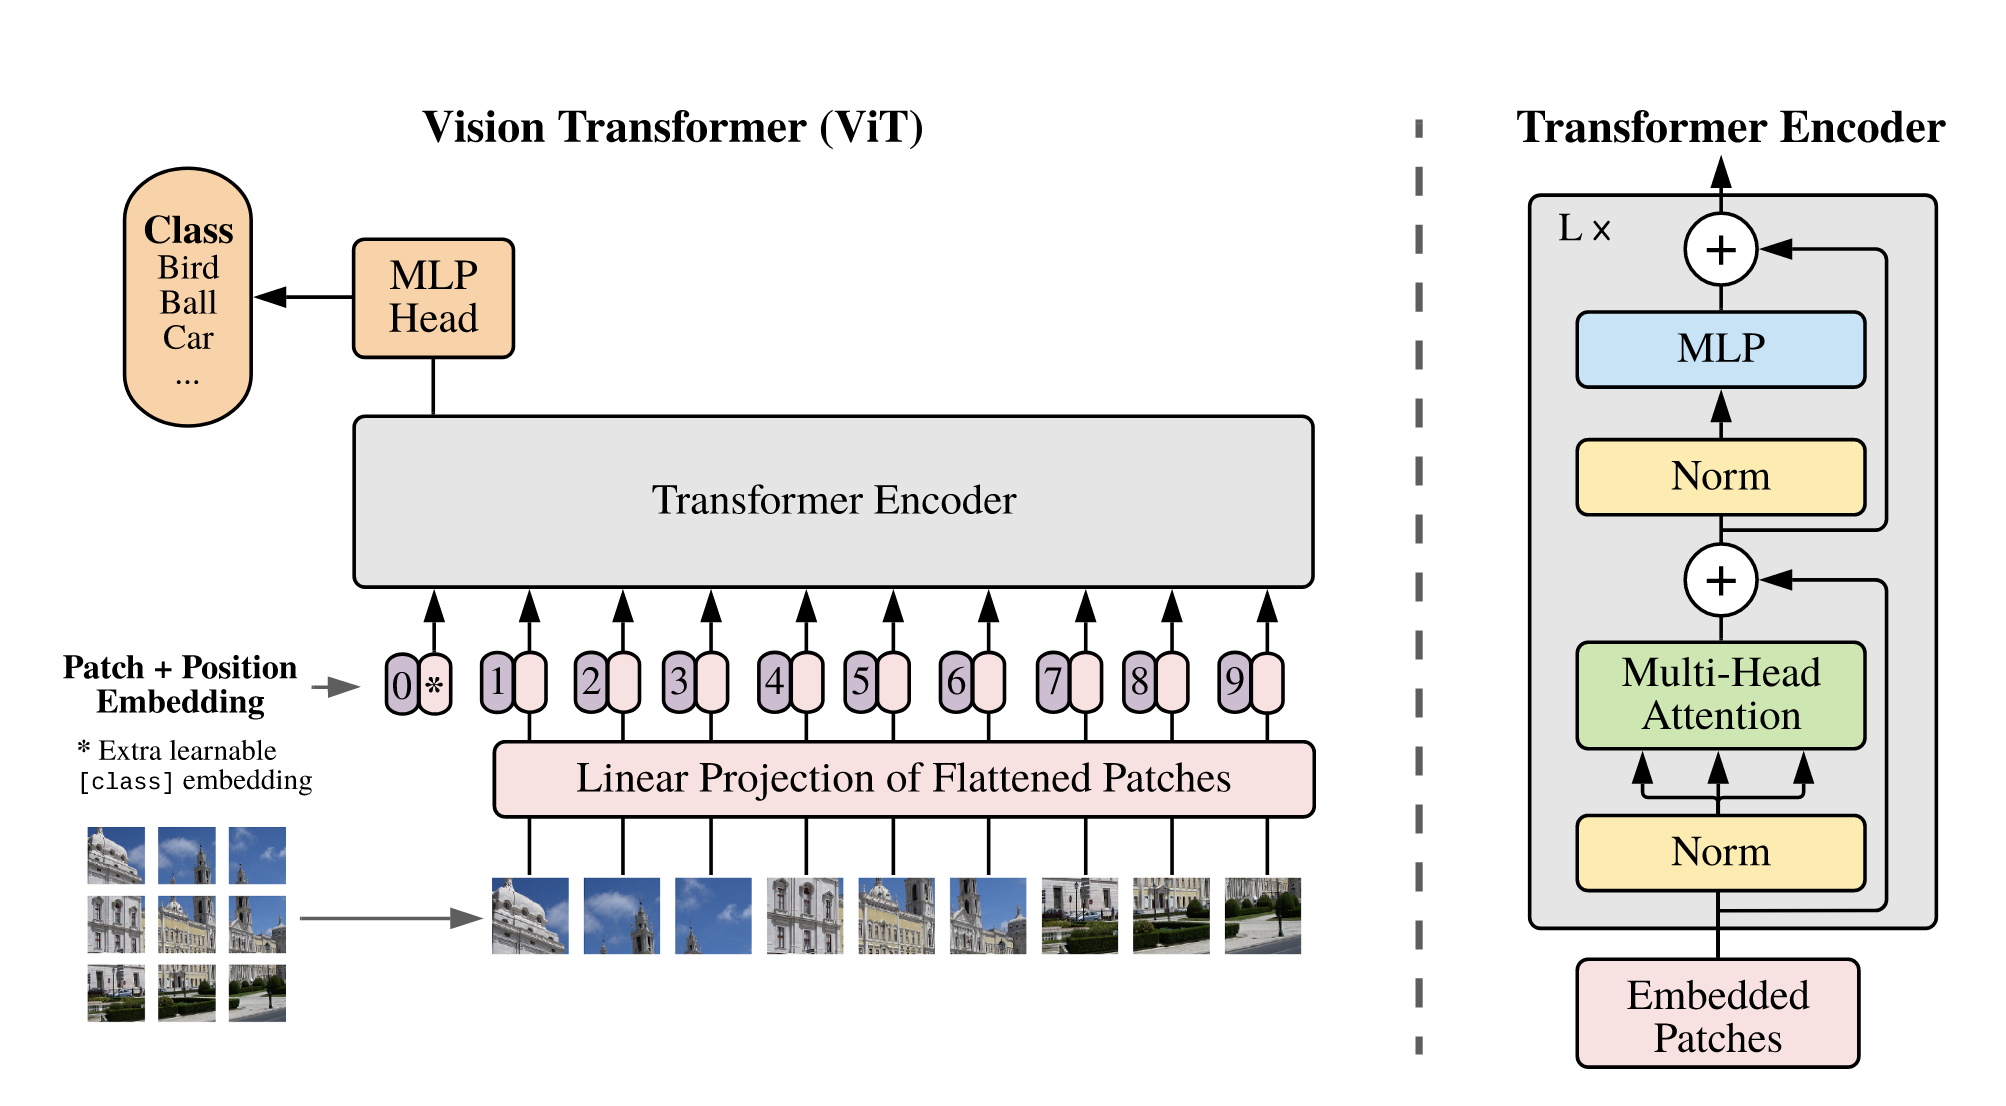
\includegraphics[width=\linewidth]{images/related/vit.png}
%       \end{center}
%       \caption{\textbf{The Vision Transformer (ViT):} the image is cropped without overlap and
%             projected using a convolution whose stride equals the kernel size. A learned ``class
%             token`` is concatenated to the resulting patches, which are then summed with a position
%             embedding. The encoder is made of multiple transformer blocks. Each block is made of two
%             (Layer) Norm layers, a MLP with a single hidden layer, and the Multi-Head Attention
%             block. Finally, only the special ``class token'' is used at the end, and fed to a
%             classifier (here denoted as the ``MLP Head''). Image from \citet{dosovitskiy2020vit}.}
%       \label{fig:related_vit}
% \end{figure}

% This architecture is illustrated in \autoref{fig:related_vit}: we concatenate a special learned
% token, called ``\textit{class token}'', to the patch tokens. Moreover, we also sum these tokens with
% a position embedding to facilitate learning tokens position. Then, successive
% transformer blocks process all the tokens. Each block is made of LayerNorms \citep{ba2016layernorm},
% a self-attention block, a \ac{MLP}, and residual connections. Thus, the self-attention block is:
% %
% \begin{equation}
%       \begin{aligned}
%             Q & =W_{q} \vx\,,                                                       \\
%             K & =W_{k} \vx\,,                                                       \\
%             V & =W_{v} \vx\,,                                                       \\
%             A & =\operatorname{Softmax}\left(Q \cdot K^{T} / \sqrt{D / h}\right)\,, \\
%             O & = W_{o} A V+b_{o}\,,
%       \end{aligned}
%       \label{eq:related_sa}
% \end{equation}
% %
% \noindent $\vx$ are the $N$ patch tokens and the class token, of shape $(N, D)$, $D$ being the
% embedding dimension. The patch tokens are linearly transformed three times in parallel into a
% \textbf{Q}uery, \textbf{K}ey, and \textbf{V}alue. An attention matrix $A$ of shape $(N, N)$ is
% computed from the query $Q$ and the key $K$. Its $i^{\text{th}}$ row contains the similarity between
% the $i^{\text{th}}$ token with all other tokens. Finally, the multiplication between the attention
% matrix and the value matrix $V$ averages all tokens according to their similarities. To extend the
% self-attention to its multi-heads variation (\ac{MHSA}), we use several Query/Key/Value
% transformations, each used in a self-attention on a fraction of the embedding dimension.

% ViT \citep{dosovitskiy2020vit} is the seminal paper on vision transformer. However, its training was
% difficult and needed a large --- and private --- dataset called JFT300M. Later works, including DeiT
% \citep{touvron2021deit} proposed an efficient optimization procedure enabling the training of
% transformers on smaller datasets such as ImageNet \citep{russakovsky2015imagenet_ilsvrc}. Finally,
% multiple works improved also the architecture itself, including CaiT \citep{touvron2021cait}, ConViT
% \citep{dascoli2021convit}, and Swin \citep{liu2021swin}. Notably, PerceiverIO
% \citep{jaegle2021perceiverio} proposed a general architecture whose output is adapted to different
% modalities using specific learned tokens, and whose computation is reduced using a small number of
% latent tokens.

% \section{Continual Learning}
% \label{sec:related_continual}

% Usually, when training a \ac{ConvNet}, we assume the dataset is immutable and \textit{i.i.d.}: no new
% images nor new classes will be learned. The knowledge acquired on one dataset \textit{A} can be
% \textit{transferred} to another dataset \textit{B} with different classes using \textbf{transfer learning}
% \citep{razavian2014transferlearning}. Then, the new model may be efficient on
% the classes of dataset \textit{B} but cannot predict anymore the classes of dataset \textit{A}.

% \textbf{Continual Learning} aims to learn a continually changing dataset without forgetting the
% previous knowledge. The distribution of the dataset continually changes: \eg at each time-step $t
%       \in \{1, ..., T \}$, new
% classes or new samples from potentially new domains are added to the training dataset
% \citep{lomonaco2017core50}. We usually assume the test dataset evolves similarly. Multiple
% distribution drifts exist in Continual Learning
% \citep{morenotorresa2012datasetshift,lesort2021driftanalysis}, and they have been called under
% various names in the literature. Given an input sample $x$ and its ground-truth $y$ (a label in
% image classification, or a segmentation map in semantic segmentation), the major drifts are:

% \begin{itemize}
%       \item \textbf{Covariate drift}: when $p(x)$ changes, it happens with the introduction of new
%             domains \citep{volpi2021continualdomainadapt}.
%       \item \textbf{Prior drift}: when $p(y)$ changes; \ac{CIL} happens with this kind of drift.
%       \item \textbf{Conceptual drift}: when $p(y | x)$ changes. Seldom covered in the literature, it
%             can be found in \acf{CSS}.
% \end{itemize}

% Learning an ever-growing dataset is possible by training from scratch a new model on the union of
% past and new data. However, for multiple reasons like privacy concerns, limited time, or small
% storage capacity \citep{vasquez2017incrementalneuralforest}, there is a restriction on the amount of
% previous data that can be kept. In the extreme case, a model only has access to new data but not old
% data. Evidently, if the initialization of the parameters is random, the model cannot predict
% the past data distribution. However, the new model parameters can be initialized using the
% previous parameters ($\theta^{t} := \theta_*^{t-1}$). Remark, from \autoref{eq:intro_optim}, that
% the optimization procedure of the old ($t-1$) and new ($t$) model is different. Given the average
% loss $L(f_\theta, \mathbb{D}) = \nicefrac{1}{|\mathbb{D}|}\sum_{(\vx,y)\in \mathbb{D}}
%       \mcL(f_{\theta}(\vx), y)$:
% %
% \begin{equation}
%       \begin{aligned}
%             \theta_*^{t-1} & = \operatorname{argmin}_{\theta^{t-1}} \left\{ L(f_{\theta^{t-1}}, \mathbb{D}^{t-1})\right \}\,, \\
%             \theta_*^{t}   & = \operatorname{argmin}_{\theta^{t}} \left\{ L(f_{\theta^{t}}, \mathbb{D}^{t})\right \}\,,       \\
%       \end{aligned}
%       \label{eq:intro_forgetting_weights}
% \end{equation}
% %
% where the loss is minimized respectively with respect to the old ($\mathbb{D}^{t-1}$) and new
% dataset ($\mathbb{D}^{t}$). Evidently, the optimal parameters $\theta_*$ are different for the task
% $t$ and $t-1$. This difference results in what we call a \textit{forgetting}: $\theta_*^t$ is
% optimal for the new task $t$ but is suboptimal for the task $t-1$, therefore performance on the
% previous task may be degraded ($L(f_{\theta^{t}}, \mathbb{D}^{t-1}) \gg L(f_{\theta^{t-1}},
%       \mathbb{D}^{t-1})$). This performance drop is actually so important that the literature names it a
% \textbf{Catastrophic Forgetting} \citep{robins1995catastrophicforgetting}. It is particularly
% critical in the context of image classification where each new task brings new classes to be
% classified as described below.

% \begin{figure}[tb]
%       \begin{center}
%             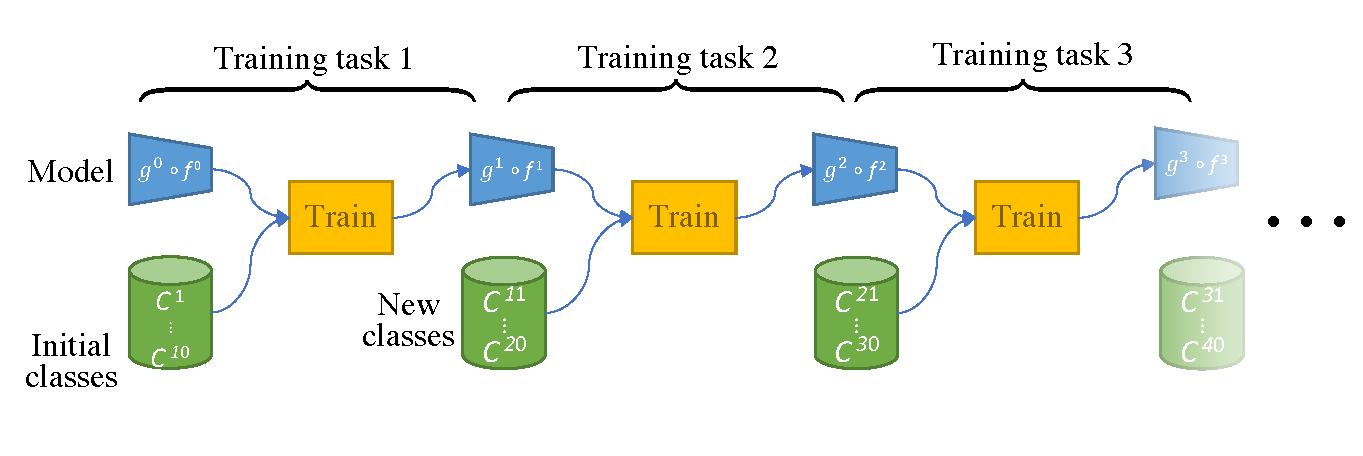
\includegraphics[width=1.0\linewidth]{images/related/protocol}
%       \end{center}
%       \caption{\textbf{Training protocol for incremental learning}. At each training task we learn a
%             new set of classes, and the model must retain knowledge about \textit{all} classes. The
%             model is allowed a \textit{limited} memory of samples of old classes.}
%       \label{fig:related_protocol}
% \end{figure}

% \paragraph{Class-Incremental Example} More concretely, a common benchmark in \acf{CIL} is learning
% the image classification CIFAR100 dataset \citep{krizhevskycifar100}, made of 100 classes, in
% multiple steps, each made of several new classes. During the first step $t=1$, the model $g^1 \circ
%       f^1$ learns the first 10 classes $\mcC^{t=1}$. During the second step $t=2$, the model $g^2 \circ
%       f^2$ is initialized from the learned parameters of the previous model $g^1 \circ f^1$ and learns the
% next 10 classes $\mcC^{t=2}$., and so on, until all 100 classes are learned at the last step $t=T$.
% After each step, we evaluate the model on the testing data of all seen classes $\mcC^{1:t}$.
% \autoref{fig:related_protocol} illustrates such continual protocol, and
% \autoref{fig:related_forgetting} depicts the continual performance of a both trained from scratch on
% all data for each task and a continual model finetuned only on new data. The continual model
% over-predicts new classes \citep{davidson2020masteryincremental} and has a low overall accuracy due
% to a forgetting of old classes. This clearly illustrates how important is the catastrophic
% forgetting. While in this thesis we mainly tackle \acf{CIL} benchmarks, we describe other continual
% benchmarks in detail in the appendix (\autoref{sec:related_variation}).

% \begin{figure}[tb]
%       \begin{center}
%             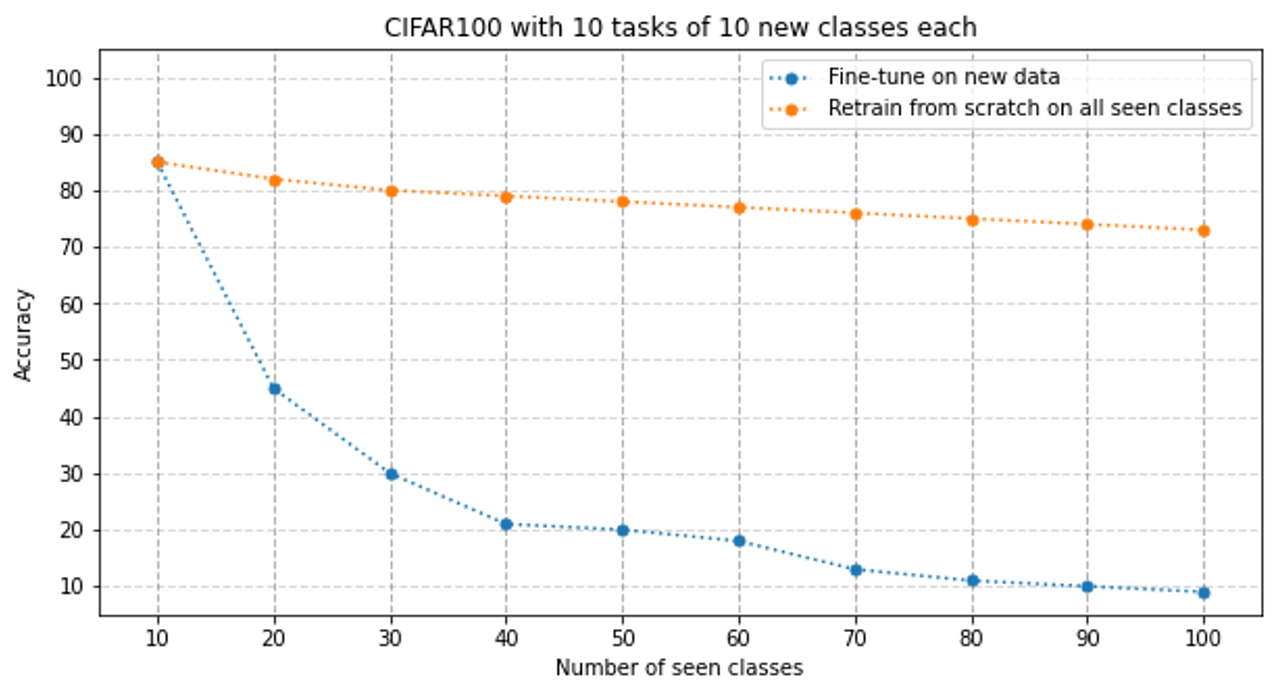
\includegraphics[width=0.8\linewidth]{images/related/catastrophic_forgetting.png}
%       \end{center}
%       \caption{\textbf{Illustration of the forgetting in Class-Incremental Learning}.
%             \textcolor{orange}{orange} line displays the accuracy of a model which is re-trained from
%             scratch at each step on all previous training data $\mcC^{1:t}$. This model, usually called
%             Joint, is considered as a reasonable upper bound. On the other hand, the
%             \textcolor{blue}{blue} line is a model finetuned solely on new classes $\mcC^{t}$ without
%             access to previous classes $\mcC^{1:t-1}$. The gap between both models illustrates the
%             catastrophic forgetting.}
%       \label{fig:related_forgetting}
% \end{figure}

% \paragraph{Single-Head \vs Multi-Heads} are the two main evaluation settings in Continual Learning
% \citep{chaudhry2018riemannien_walk}. In the former setting, a model has to classify samples among
% all seen classes $\mcC^{1:t}$, that could have been learned from any of the seen steps. On the other
% hand, in a multi-heads setting, a model knows at test-time the step/task identifier $i$ of the
% samples. Thus, it only has to classify among the limited number of classes brought by a step
% ($\mcC^i$). Multi-Heads evaluation is closely related to multi-tasks learning. During this thesis,
% we focus on the Single-Head evaluation because it is more realistic as it is rarely possible to know
% from which step a sample comes from in a real-life setting. This setting is also more challenging
% because a unique classifier must discriminate among all tasks' classes instead of having a different
% classifier per task \citep{lesort2019regulshortcomings}.


% %\subsection{Metrics for Continual Learning}
% \label{sec:related_metrics}

% \paragraph{Metrics} Multiple metrics exist in Continual Learning: the most common are the
% \textbf{final accuracy} and \textbf{average incremental accuracy}. The former measures the
% performance of the model on all tasks at the last step, the latter measures the average of
% performance on all seen tasks after each new task learned \citep{rebuffi2017icarl}. Practically,
% given $A_{i,t}$ the accuracy of the $i^{th}$ task after learning the $t^{th}$ task, the final
% accuracy is (assuming balanced tasks):
% %
% \begin{equation}
%       \text{Acc}_F = \frac{1}{T} \sum_{i=1}^T A_{i,T}\,,
%       \label{eq:related_final_acc}
% \end{equation}
% %
% and the average incremental accuracy:
% %
% \begin{equation}
%       \text{Acc}_a = \frac{1}{T} \sum_{t=1}^T \frac{1}{t}  \sum_{i=1}^t A_{i,t}\,.
%       \label{eq:related_avg_acc}
% \end{equation}
% %
% Average incremental accuracy is somewhat more important than simply the final accuracy: a continual
% model should be good after every step because in a true continual setting, there is not a ``final
% task''.

% Other metrics exist \citep{diaz2018continualmetrics}, such as \textbf{forgetting}
% \citep{chaudhry2018riemannien_walk} which records how much a model has lost performance-wise on a
% task compared to the first time it has learned it. The interest of this metric is to be agnostic of
% the absolute performance of the model used.

% Finally, metrics such as \textbf{speed} (\ie the number of images processed per second) or used
% \textbf{capacity} (\ie number of learned parameters) are important:
% \citet{ramasesh2022scalecontinual} recently showed that the larger a model was the lower was the
% forgetting.

% \section{Methods to reduce forgetting}
% \label{sec:related_methods}

% Multiple approaches exist to reduce forgetting in Continual Learning. The major ones are
% rehearsal of old data (\autoref{sec:related_rehearsal}), regularizations constraining the model's
% behavior (\autoref{sec:related_regul}), and structural adaptations (\autoref{sec:related_structural}).

% \subsection{Rehearsal Learning}
% \label{sec:related_rehearsal}

% The most efficient method to reduce forgetting is \textbf{rehearsal learning} where old samples will
% be seen alongside the new samples. The amount of old samples stored is extremely limited, otherwise,
% it would defeat the purpose of continual learning. \autoref{fig:related_protocol_rehearsal} illustrates how
% rehearsal learning happens in Continual Learning. During the first step, a model is trained on all
% available samples. Then, it stores a limited amount of those in a \textit{memory}. During the second
% step, the model has access to new samples but also all samples stored in the memory. In
% Class-Incremental, an equal amount of samples per class is stored in memory. There are
% two major approaches to determine this amount: \citet{rebuffi2017icarl} propose to fully use a
% memory of size $\mcM$ among all $\mcC$, while \citet{hou2019ucir} instead kept fixed the number of
% samples stored per class to $\nicefrac{\mcM}{|\mcC^{1:T}|}$.

% \begin{figure}[tb]
%       \begin{center}
%             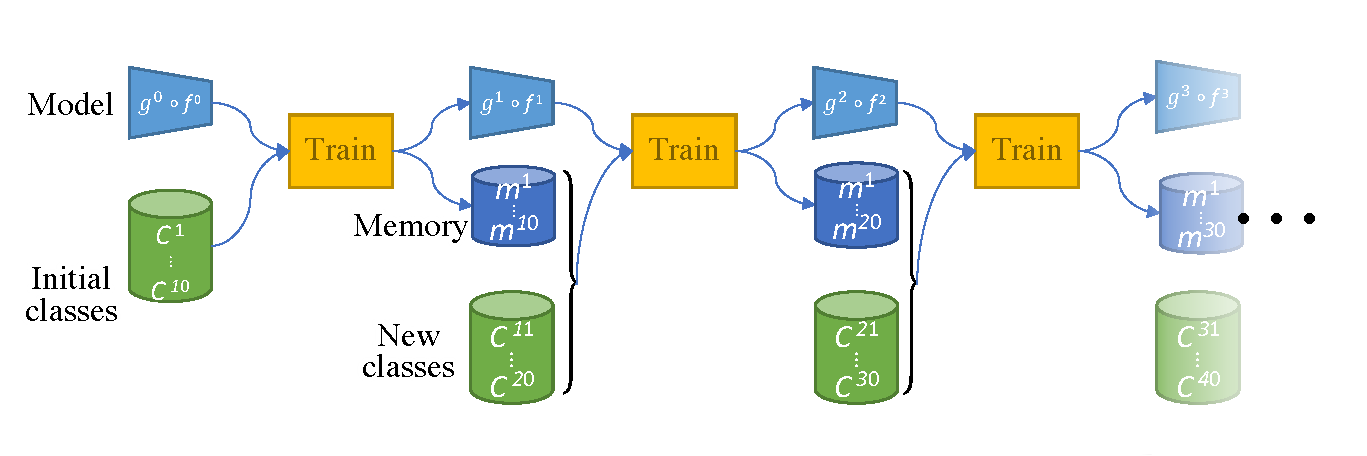
\includegraphics[width=1.0\linewidth]{images/related/rehearsal}
%       \end{center}
%       \caption{\textbf{Training with a rehearsal memory}. After each task a fraction of the
%             data is stored in a memory to be used in the next task. Rehearsal learning is the most
%             efficient method to reduce forgetting, but unfortunately the memory capacity is often
%             extremely limited.}
%       \label{fig:related_protocol_rehearsal}
% \end{figure}

% \paragraph{Herding} is the action of choosing which samples per class to store in the rehearsal
% memory. The most naive herding method is to randomly sample images. Despite its simplicity, it is
% quite competitive with more complex method \citep{castro2018end_to_end_inc_learn}, echoing similar
% results in \ac{AL} \citep{gal2017activelearning}. Other herding methods include fetching samples
% close to the class mean in the feature space \citep{castro2018end_to_end_inc_learn} or close to an
% incremental barycenter \citep{rebuffi2017icarl}.

% \paragraph{Sampling} is an important but yet fewly investigated topic in Continual Learning. Most
% models mix all memory samples with new samples without any under- or over-sampling.
% \citet{castro2018end_to_end_inc_learn} propose to finetune for a few epochs, after training on a new
% step, on a balanced set of old and new classes samples. \citet{chaudhry2019tinyepisodicmemories}
% oversample tiny memory with as low as one sample per class, and show, in the context of Online
% Learning where models learn in only one epoch, that continual models still do not overfit. In the
% same context, \citet{aljundi2019maximallyinterfered} propose to over-sample the memory examples with
% the highest losses. In an imbalanced situation for Continual Learning, over- and under-sampling can be
% applied depending on the number of samples per class \citep{kim2020imbalancedcontinual}.

% \paragraph{Efficient Storing} is important for rehearsal learning: a bigger rehearsal memory leads
% invariably to less forgetting \citep{hou2019ucir}. Thus, multiple works consider how to store more
% rehearsal samples given the same memory size: \citet{hayes2020remind} compress intermediate features
% of memory samples with a lossless compression algorithm.
% \citet{iscen2020incrementalfeatureadaptation} also store features but modify them through the
% training to handle the inherent internal covariate drift.

% \paragraph{Pseudo-rehearsal} does not need to store samples but instead generates pseudo-samples for
% rehearsal \citep{lesort2019generative}. The generation can be done with auto-encoders from
% intermediate features \citep{kemker2018fearnet,ayub2021eec} or use \ac{GAN}
% \citep{shin2017deep_generative_replay}. Unfortunately, those methods have several drawbacks: they
% struggle to scale to large images, the generator size may be superior to a classic rehearsal memory
% size which would defeat the goal of using less storage, and finally, the generator may itself suffer
% from catastrophic forgetting \citep{zhai2019lifelonggan}. \citet{liu2020mnemonics} propose instead a
% method halfway between rehearsal and pseudo-rehearsal: the authors randomly sample real images, and
% then during continual training, slightly modify them via bi-level optimization
% \citep{wang2018datasetdistillation} to minimize forgetting.


% \subsection{Regularization-based Approaches}
% \label{sec:related_regul}


% \begin{figure}[tb]
%       \begin{center}
%             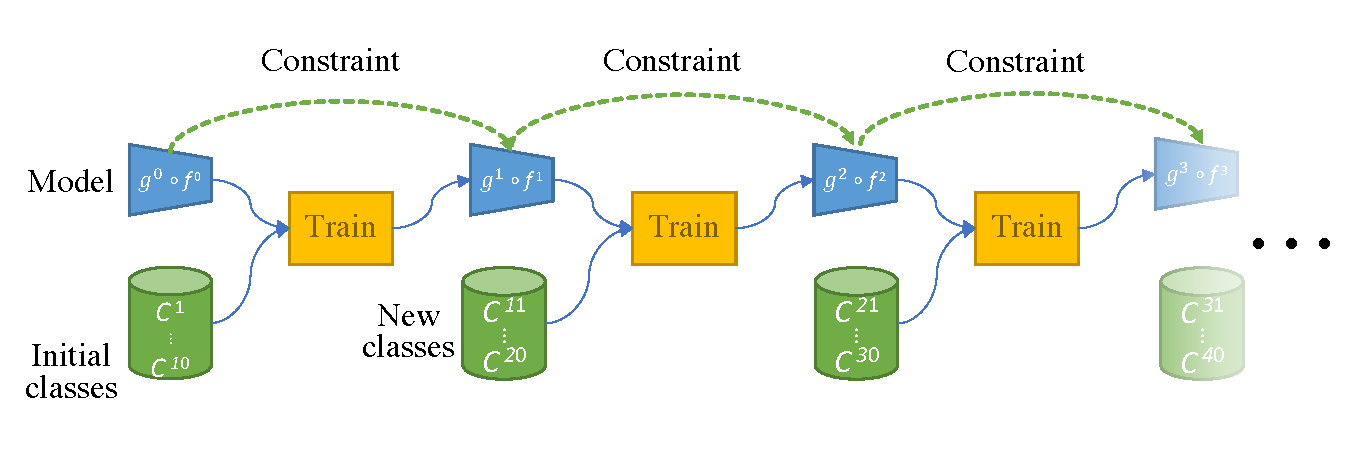
\includegraphics[width=1.0\linewidth]{images/related/constraints}
%       \end{center}
%       \caption{\textbf{Constraining the new model based on the old model}. During each task, after
%             the first one, the new model is constrained to be similar to the old model in order to reduce
%             forgetting.}
%       \label{fig:related_protocol_constraints}
% \end{figure}

% A common and efficient way to reduce forgetting is to minimize the difference in behavior between
% the old and new models as illustrated in \autoref{fig:related_protocol_constraints}. These constraints can be
% expressed through various forms and are described below.

% \subsubsection{Weight-based constraints}
% \label{sec:related_regul_weight}


% The most straightforward way to avoid completely forgetting is that the old and new models stay
% identical. While the model would be \textit{rigid} (no forgetting), it is also not \textit{plastic}
% (changing a lot) at all, and thus cannot learn any new tasks. Thus, a line of research proposed to
% constrain only a portion of the neurons:
% %
% \begin{equation}
%       \mcL(\theta^t, \theta^{t-1}) = \mcL_t(\theta^t) + \lambda \sum_i \Omega_i^{t-1} (\theta^t_i - \theta_i^{t-1})^2\,,
%       \label{eq:related_weight_constraint}
% \end{equation}
% %
% where $\mcL_t(\theta)$ is the loss at the current task $t$ (\eg the cross-entropy), $\theta_i^t$
% and $\theta_i^{t-1}$ respectively the $i^\text{th}$ neuron of the current and previous model, and
% $\Omega_i^{t-1}$ a neuron-wise importance factor. The intuition is that important neuron for the
% previous task $t-1$ should not change, while the others can be adapted to fit the new task $t$.

% \citet{kirkpatrick2017ewc}, followed by \citet{zenke2017synaptic_intelligence} and
% \citet{chaudhry2018riemannien_walk} propose to use the diagonal Fisher information matrix as
% importance factors. The motivation behind was that the posterior $p(\theta^{t-1} | \mcD^{t-1})$ must
% contain the information about which parameters are important to the previous dataset $\mcD^{t-1}$.
% This posterior can be approximated by a Gaussian distribution whose diagonal precision is given by
% diagonal Fisher information matrix. A higher value means a more important neuron for the previous
% task, and thus the constraint should be increased proportionally. Thus, a lower value, for a less
% important neuron, means that it can change drastically, which would facilitate learning new data.
% This strikes a balance between rigidity (not changing and thus not forgetting), and plasticity
% (changing, and thus learning new concepts). Note that \citet{aljundi2018MemoryAwareSynapses} instead
% use the sensitivity of the model when small perturbations are added to the neurons to measure their
% importance.

% However, it is worth remarking that weight-based constraints are usually limited to the multi-heads
% setting where a task identifier is available at test time. \citet{lesort2019regulshortcomings} show
% that in the single-head setting, they struggle to reduce forgetting and are significantly
% outperformed by the simple (but somewhat memory costly) rehearsal learning.

% \subsubsection{Gradient-Based methods}
% \label{sec:related_regul_gradient}

% \begin{figure}[tb]
%       \begin{center}
%             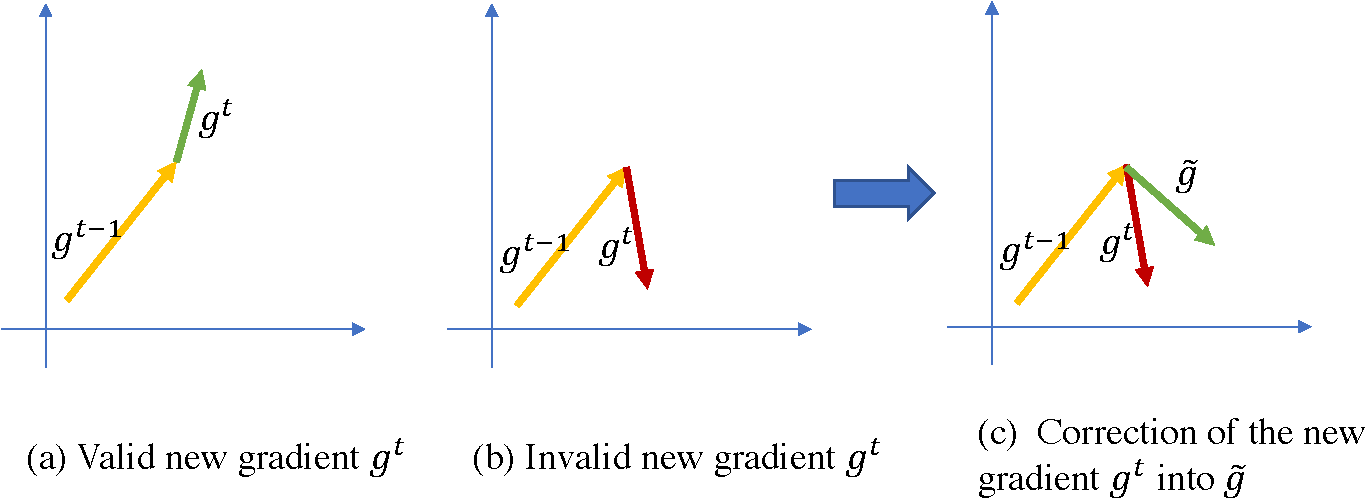
\includegraphics[width=1.0\linewidth]{images/related/gem.pdf}
%       \end{center}
%       \caption{\textbf{GEM's gradient constraint} forcing updates to be in the same direction as the
%             gradient \wrt old samples. In (a) the new gradient $g^t$ is valid, while in (b) the new gradient
%             violates the constraint of $\langle g^t,\, g_{t-1}\rangle \ge 0$. In (c), the invalid gradient
%             $g^t$ is projected to the closest valid alternative $\tilde{g}$.}
%       \label{fig:related_gem}
% \end{figure}

% \citet{lopezpaz2017gem} propose the GEM model that combines a constraint on the gradients and
% rehearsal learning. The algorithm requires that the loss on a given stored sample must not increase
% despite the model learning new classes. The authors, given a locality assumption, rewrite this
% formulation as enforcing that the gradient of a new sample ($g$) to be in the same \textit{direction} as
% the gradient of all stored old samples ($g_i \, \text{for all}\, i \in \mcM$):
% %
% \begin{equation}
%       \langle g,\, g_i\rangle \ge 0,\, \text{for all}\, i \in \mcM\,,
% \end{equation}
% %
% \noindent with $\mcM$ the rehearsal memory. If the constraint is violated, the new gradient $g$ is
% projected to the closest in L2 norm gradient that satisfies the angle constraint by minimizing a
% quadratic program. The constraint is illustrated in \autoref{fig:related_gem}. The drawback of this
% method is the computational cost that can grow prohibitively when the memory is too large.
% \citet{chaudhry2019AGEM} propose Averaged-GEM to speed up GEM: the authors do not constraint the
% gradient of individual memory samples but only the average of all memory samples.
% \citet{aljundi2019gradientselection} also improved GEM's speed by selecting only a subset of the
% memory samples that maximize the feasible region.

% Differently, but still constraining the gradients: \citet{farajtabar2020ogd}'s OGD forces the gradients of
% task $t$ to be orthogonal to gradients of task $t-1$. They use the Gram-Schmidt procedure to
% orthogonalize the new gradients, allowing updates for the new task that minimally interfere with the
% performance of old tasks. \citet{saha2021gpm}'s GPM does likewise but uses instead a k-rank
% approximation of the SVD of the representation matrix.


% \subsubsection{Output-based constraints regularizations}
% \label{sec:related_regul_output}

% Finally, the majority of Continual models that are benchmarked on large datasets (\eg ImageNet
% \citep{deng2009imagenet}) use a combination of rehearsal
% learning (\autoref{sec:related_rehearsal}) and constraints on the model's outputs.

% LwF \citep{li2018lwf} and iCaRL \citep{rebuffi2017icarl} apply the \ac{KD}
% \citep{hinton2015knowledge_distillation} on the model's probabilities. It usually consists in
% minimizing the \ac{KL} between the probabilities of the old and new models:
% %
% \begin{equation}
%       \mcL_\text{KD} = \operatorname{KL}(\operatorname{softmax}(\frac{\tilde{y}^{t-1}}{\tau}) \Vert \operatorname{softmax}(\frac{\tilde{y}^t}{\tau})\,,
% \end{equation}
% %
% where $\tilde{y}^{t-1} = g^{t-1} (f^{t-1}(\vx))$ and $\tilde{y}^{t} = = g^{t} (f^{t}(\vx))$ are respectively the logits of the old and new model,
% and $\tau$ a \textit{temperature} to soften the probabilities in order to give more importance to
% the model confidence in other classes than the top one. These probabilities, nicknamed \textit{dark
%       knowledge} by \citet{hinton2015knowledge_distillation}, contain additional information about the
% model which are useful to distil. Note that in the context of Class-Incremental, the new model
% predicts more classes than the old model, therefore, the \ac{KL} is only applied on the logits
% common to both the old and the new models. The \ac{KD} is sometimes also defined as the binary
% cross-entropy between the sigmoid-activated logits.

% Constraining the probabilities is now so ubiquitous that most models include it in their base
% losses. On the other hand, a few models considered constraining intermediate outputs. MK2D
% \citep{peng2019m2kd} uses the \ac{KD} from both the final classifier and an auxiliary classifier
% similarly to the Inception network \citep{szegedy2015inception}. \citet{hou2019ucir} maximize the
% cosine similarity between the embeddings produced by the \ac{GAP}.
% \citet{dhar2019learning_without_memorizing_gradcam} minimizes the L1 distance between the attention
% maps produced by GradCam \citep{selvaraju2017gradcam}.

% \subsection{Structural Strategies}
% \label{sec:related_structural}

% \begin{figure}[tb]
%       \begin{center}
%             {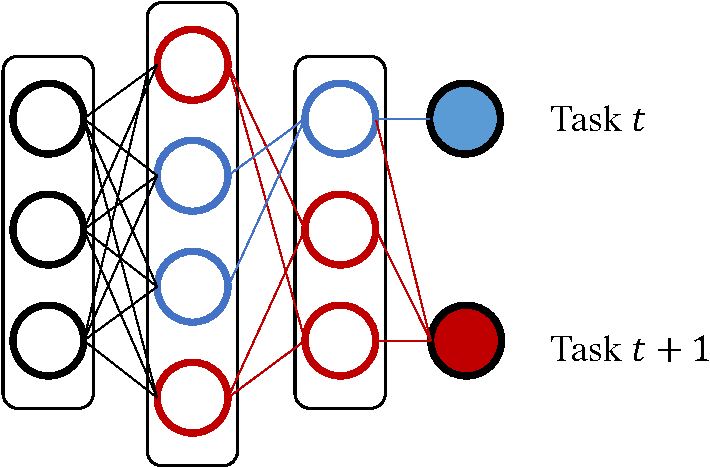
\includegraphics[width=0.5\linewidth]{images/related/subnetworks.pdf}}
%       \end{center}
%       \caption{\textbf{Task-specific subnetworks} that can be uncovered with a sparsity loss or
%             learned masking. \textcolor{blue}{\textbf{Blue}} neurons are dedicated to
%             the task $t$, \textcolor{red}{\textbf{red}} neurons to the following task
%             $t+1$, and \textbf{black} neurons are shared among all tasks. At
%             test-time, a task identifier of the sample is required to select the
%             right subnetwork path.}
%       \label{fig:related_subnetwork}
% \end{figure}

% Multiple works also propose to adopt dynamic strategies where the configuration of the neural
% network evolves after each task. Critically, not only the number of neurons changes in the classifier $g^t$
% (to incorporate new classes to predict), but the feature extractor $f^t$'s neurons count or organization
% will also differ from its previous iteration $f^{t-1}$.


% \paragraph{Subnetworks} The Lottery Ticket Hypothesis \citep{frankle2019lottery_ticket} states that
% subnetworks made of a fraction of the neurons and connections of a larger network, can reach
% excellent performance. Several Continual Learning models exploit that property by using a
% subnetwork per task. Those subnetworks can be uncovered via genetic algorithms
% \citep{fernando2017path_net}, via induced L1 sparsity \citep{golkar2019neural_pruning}, or even
% learned masked \citet{serra2018hat,hung2019cpg}. Usually, these methods require a task identifier at
% test-time in order to select the right subnetwork (see \textit{multi-heads} in
% \autoref{sec:related_continual}). Later, \citet{wortsman2020supermasks} propose to infer the task
% identifier by selecting the subnetwork with the lowest entropy. This subnetwork-based approach is
% illustrated in \autoref{fig:related_subnetwork}.

% \paragraph{Dynamically Expandable Networks} A neural network can also be expanded through its continual
% training to accommodate the growing amount of tasks to solve. First, \citet{rusu2016progressive}
% propose to have one network per task, where the $i^{\text{th}}$ network would depend both on the
% input and all previous networks' intermediate features. Unfortunately, memory consumption is
% quickly prohibitive with many tasks. Following works propose to only add blocks of parameters,
% and only when deemed necessary \citep{veniat2021mntdp}. While these dynamic networks often require
% an identifier at test-time to select the right subset of parameters, recently, DER
% \citep{yan2021der} removed this need by learning a classifier upon the concatenated features of all tasks:
% Their dynamic expansion of the representation adds a new feature extractor per task. All
% extractors' embeddings would then be concatenated and fed to a unified classifier, discarding the
% need for a task identifier at test-time. To limit an explosion in the number of parameters, they
% aggressively prune each model after each task using the HAT \citep{serra2018hat} procedure.
% Unfortunately, the pruning is hyperparameter sensitive. Therefore, hyperparameters are tuned
% differently on each experiment: for example, learning a dataset in 10 steps or in 50 steps use
% different hyperparameters. While being impracticable, it is also unrealistic because the number of
% classes is not known in advance in a true continual situation. Simple-DER \citep{li2021preserve}
% also uses multiple extractors, but its pruning method doesn't need any hyperparameters; the negative
% counterpart is that Simple-DER controls less the parameter growth.

% \paragraph{Task Conditioning} Rather than adding many new parameters, it is also possible to only
% add a few parameters that will adapt the existing network behavior for a task.
% \citet{rebuffi2017visualadapters} propose to add a different residual per task: given a task
% identifier, the associated residual is used, and the features are modulated to best fit the given
% task. Instead of adapting the features, \citet{wen2020batchensemble} and \citet{sun2019metatransfer}
% propose to share most of the weights across tasks, but have task-specific weights that directly
% modify the shared weights.

% \paragraph{Mixture-of-Experts} Mixture of experts \citep{masoudnia2014mixture} have also been
% proposed, where multiple experts combine their decision. \citet{aljundi2017experts} learn a gating
% system to use the right task-specific expert. \citet{collier2020routingnetwork} stress the importance
% on sharing experts when tasks are similar.
% %\citet{yan2021der} and \citet{li2021preserve} proposed
% %to have a \ac{ConvNet} per task and to concatenate their output embeddings to be fed to a single
% %classifier. To avoid parameters explosion, they aggressively prune each \ac{ConvNet}.

% \paragraph{Classifier Correction} Forgetting happens in both the feature extractor and the
% classifier. Previously described rehearsal and regularization methods try to reduce it in both
% places. On the other hand, multiple works focus solely on the classifier. They remark that in
% \acf{CIL}, the classifier is miscalibrated \citep{guo2017miscalibration} where the model
% over-predicts new classes to the detriment of old classes. \citet{belouadah2019il2m} compensate the
% bias towards new classes by rectifying predictions of past classes using their recorded accuracies
% and confidences. \citet{wu2019bias_correction} learn a linear model on validation data to recalibrate
% the logits of the new classes. \citet{zhao2020weightalignement} normalizes the norm of the classifier
% weights associated with new classes so that their average norm becomes the same as that for old
% classes. \citet{hou2019ucir}, aims for a similar result by replacing the dot product in the
% classifier with the cosine similarity, resulting in unit norm classifier weights.

% \section{Positioning}

% Continual Learning encompasses very different benchmarks and methods. In this PhD thesis, we tackle
% multiple types of continual drift using different approaches. All the proposed strategies consider
% the intermediary features of a neural network to reduce catastrophic forgetting. We summarize
% below the three main chapters:

% \paragraph{Feature-based Regularizations} First in \autoref{chapter:regularization}, we consider
% \acf{CIL} scenarios with a prior drift where new classes are continually added. In this setting, our
% approach consists in rehearsal learning (\autoref{sec:related_rehearsal}) and output-based
% regularizations (\autoref{sec:related_regul_output}). Previous works reduced forgetting by
% constraining either the final probabilities of the classifier \citep{li2018lwf} or the ultimate
% embedding of the feature extractor \citep{hou2019ucir,dhar2019learning_without_memorizing_gradcam}.
% In a first section (\autoref{sec:podnet}), we propose instead a regularization applied on several
% intermediary levels of the features extractor. Moreover, few considerations have been made on how
% the regularization loss makes the model more rigid, leading to less forgetting on old classes but
% also impacting negatively the learning of new classes. Instead, we carefully define a regularization
% loss, through pooling, balance effectively the performance of old and new classes. In a second
% section (\autoref{sec:ghost}), we consider if the forgetting could be avoided preemptively.
% \citet{aljundi2019selfless} consider allocating extra capacity implicitly in the learned feature
% space for future classes using an unsupervised sparsity loss. Differently, we choose to draw from
% weak metadata of the future unseen classes \citep{hanrebuffi2020autodiscovering} to estimate their
% representation and thus explicitly allocate capacity, reducing forgetting before it even happens.

% \paragraph{Continual Semantic Segmentation} Second, in \autoref{chapter:segmentation}, we tackle
% \acf{CSS}. In this benchmark, defined recently by \citet{cermelli2020modelingthebackground}, images
% have a label per pixel, and only the current classes are labelized. Thus, both the prior and concept
% drifts happen where new classes are added but also the signification of a pixel can change through
% time. In this setting, all previous works only considered regularizations
% (\autoref{sec:related_regul_output}) based on the final probabilities
% \citep{michieli2019ilt,cermelli2020modelingthebackground}. Instead, we expand from our previous
% chapter to consider the multi-scale intermediary features. Moreover, no work directly tackled the
% partial labelization of the images \citep{cermelli2020modelingthebackground}. We propose for this
% challenge an uncertainty-based pseudo-labeling \citep{saporta2020esl}, and a new rehearsal method
% (\autoref{sec:related_rehearsal}), optimized for segmentation.

% \paragraph{Dynamic Transformers} In this third and last chapter (\autoref{chapter:dynamic}), we only
% aim to solve the prior drift but using a method radically different from previous chapters: dynamic
% networks (\autoref{sec:related_structural}). Previous dynamic networks usually expand their capacity
% by a large margin during the continual training to handle the growing amount of tasks to learn
% \citep{yan2021der}. To avoid a parameter count unbounded growth, the models are usually pruned
% aggressively. The main drawback of these methods is that the pruning can still result in models too
% large and often need careful finetuning of hyperparameters. We propose in this chapter, a dynamic
% expansion based on the transformer architecture with almost no memory overhead contrary to
% concurrent works, that conditions \citep{perez2018film} the intermediary features.

\cleardoublepage
\let\leftmark=\oldleftmark


\acresetall
\chapter{Editing images with a pre-trained GAN}
\label{chapter:magec}

\newpage
\minitoc

%\newcommand{\mcL}{\mathcal{L}} \newcommand{\vx}{\mathbf{x}} \newcommand{\vh}{\mathbf{h}}
%\newcommand{\vy}{\mathbf{y}}
\newcommand{\tableindent}{\,\,\,\,}
\newcommand{\vt}{\mathbf{t}}
%\newcommand{\vyh}{\hat\vy}
\newcommand{\std}{$\pm\,$}
\newcommand{\clf}{\textit{clf}} \newcommand{\gray}[1]{{\color{darkgray}#1}}





% \begin{chapabstract}
%     abstract

% \end{chapabstract}
% \newpage

% \minitoc

\chapterwithfigures{\nameref*{chapter:magec}}
\chapterwithtables{\nameref*{chapter:magec}}

\ifthenelse{\boolean{skipMagec}}{\endinput}{}

\todo{fix chapter:related bus}

\section{Introduction}

In this chapter, we abord the question of image editing with a pre-trained deep \ac{GAN}.
For the first time, \ac{DL} models, specifically \ac{GAN}s, have achieved photorealistic synthesis \citep{karras2018progressive, karra2019stylegan, karra2020stylegan2}.
Moreoever, as discussed in Chapter \ref{chapter:related}, methods have recently emerged to 
have semantic control of the generation via clever ways of manipulating the latent vector \citep{shen2020, abdal2020styleflow, harkonen2020ganspace, tewari2020stylerig, stylespace_analysis, zhuang2021enjoy, editing_style}.
 These editing methods also produce photorealistic images, contrary to concurrent image-to-image models which 
produce noticable artificats (albeit being more controllable) \citep{wang2018pix2pixHD, park2019gaugan}.
 In the context of image editing for the general public, latent space manipulation with the latest 
 StyleGAN2 network \citep{karra2020stylegan2}
is thus an inticing area to experiment with. 

% Generative Adversarial Networks (GANs) \cite{goodfellowgans} have made such ideas 
% possible in recent years. Recently, the celebrated StyleGAN \cite{karra2019stylegan, karra2020stylegan2} 
% has allowed unconditional generation of unparalleled quality, resolution ($1024 \times 1024$) and 
% realism. What's more, this GAN was the first of its kind to show such powerful 
% \emph{disentanglement qualities} of its latent space. For example, mixing two latent codes
%  corresponding to two images results in a coherent output image containing properties from 
%  both former images  \cite{karra2019stylegan}. This led to a surge of research into studying 
%  and manipulating this latent space, in which high-level semantic concepts  of generated images 
%  can be edited \cite{shen2020, abdal2020styleflow, harkonen2020ganspace, tewari2020stylerig, stylespace_analysis, zhuang2021enjoy, editing_style}. 
%  These editing methods produce realistic and high-quality global or local changes in the output image.

The extension to real images is natural but not trivial. A latent code first needs to be 
found such that, when inserted into the StyleGAN network, outputs the original image, a process
known as \emph{GAN inversion}.
Although inversions are able to achieve high reconstruction quality  
\citep{abdal2019image2stylegan, abdal2020}, problems arise when applying known editing methods 
onto the inverted images: the editing either does not work at all, or they produce output 
images of poor quality, presenting artifacts and blur \citep{zhu2020indomain, StyleGAN3D}. 
 We examine the reasoning behind this lack of generalization and propose a solution to this problem 
 by reframing the standard optimization framework for GAN inversion specifically in the lense of 
 editability of the reconstructed image. More precisely, we introduce a term of editability
 and i\textbf{MAG}e-lat\textbf{E}nt \textbf{C}onsistency (dubbed ``\magec'') into the global 
 loss function by using a simple yet effective procedure based on recent latent-manipulation methods.
 This allows us to explicitly incorporate 
 known editing methods into the GAN inversion optimization scheme to ensure better editability. \todo{matt's comment}
We validate our method with extensive qualitative and quantitative evaluation. Notably, we 
introduce a novel ``edit-consistency score'' which specifically evaluates the quality of a projection
method in terms of editability. We show that our method outperforms existing baseline methods, and
 opens the door to new possibilities of editable high-quality image inversions.

%  We introduce an i\textbf{MAG}e-lat\textbf{E}nt \textbf{C}onsistency (``\textbf{MAGEC}'') loss 
% during the inversion process. This specifically incorporates editability into the inversion
%  loss alongside with the reconstruction loss, 
% which achieves an faithful and editable reconstruction.

% In this paper, we propose a learning framework to improve editability of the projected latent 
% vector of a real image while maintaining good reconstruction. We reframe the strategy of the
%  standard optimization framework for GAN inversion. More precisely, we add a term of editability
%   and image-latent-consistency into the global loss function by using a simple yet effective 
%   procedure based on recent latent-manipulation methods. This allows us to explicitly incorporate 
%   known editing methods into the GAN inversion optimization scheme to ensure better editability. 
% We validate our method with extensive qualitative and quantitative evaluation. Notably, we 
% introduce a novel ``edit-consistency score'' which specifically evaluates the quality of a projection
%  method in terms of editability. We show that our method outperforms existing baseline methods, and
%   opens the door to new possibilities of editable high-quality image inversions.






% In this chapter, our goal was to leverage recent works on latent space manipulation 
% (see \ref{subsection:latent_space_manipulation}) to perform editing on real images. We leverage the 
% highly performant StyleGAN2 network (\ref{par:latent_space})



% We first explore real-image editing using a pre-trained \ac{GAN}. We explore the recent 
% StyleGAN (1 and 2) \citep{karra2019stylegan, karra2020stylegan2} architecutre for the specific task of real-image editing. 
% For the first time, this architecture allowed easy, fine-grained control of the generation just by cleverly modifying the values of the 
% latent vector input to the \ac{GAN}. For example, tweaking a subset of the values in this vector allows changing a specific
% characteristic of the output image, such as hair color or gender, as described in \ref{subsection:latent_space_manipulation}.
%  This type of high-level semantic editing is exactly our goal, 
% and we thus set out to apply these techniques on real images.

% In order for these methods to be applied to real images, a real image must first be inverted into the latent space of the \ac{GAN}. 
% Unfortunately, while standard inversion methods produce an accurate reconstruction of the image, they do not behave 
% well when the aforementioned latent-editing methods are applied. Indeed, the resulting image is either incorrectly 
% edited or of poor quality. We examine the reasoning behind this lack of generalization and propose a solution to this problem. Our contribution, 
% introduced in \autoref{sec:magec} introduces an i\textbf{MAG}e-lat\textbf{E}nt \textbf{C}onsistency (``\textbf{MAGEC}'') loss 
% during the inversion process. This specifically incorporates editing success into the inversion loss alongside the reconstruction loss, 
% which achieves an faithful and editable reconstruction.

% In this chapter, we will first discuss in some details the related work needed to contextualize our work.
% We go into more detail about the existing latent-space manipulation methods, introduced in \ref{subsection:latent_space_manipulation}. 
% We also discuss existing methods for GAN Inversion before detailing our own contribution to this field.



% In this paper, we propose a learning framework to improve editability of the projected 
% latent vector of a real image while maintaining good reconstruction. We reframe the strategy 
% of the standard optimization framework for GAN inversion. More precisely, we add a term of 
% editability and image-latent-consistency into the global loss function by using a simple yet 
% effective procedure based on recent latent-manipulation methods. This allows us to explicitly 
% incorporate known editing methods into the GAN inversion optimization scheme to ensure better 
% editability. 
% We validate our method with extensive qualitative and quantitative evaluation. Notably, we 
% introduce a novel ``edit-consistency score'' which specifically evaluates the quality of a 
% projection method in terms of editability. We show that our method outperforms existing baseline
%  methods, and opens the door to new possibilities of editable high-quality image inversions.





\section{Related Work}







% Editing real images in a fast and realistic way is highly lucrative for obvious reasons. 
% Users could use such a tool to visualize their personal curiosities before committing more 
% time or energy to something more permanent - How would a certain hairstyle look on me? How 
% would my house look with brick walls? Would my car look nice with different tires? Moreover, 
% a professional photographer spends around 1.5 hours of editing for a portrait image, with 
% the most costly operations being those requiring complicated semantic changes \cite{photoshop}.
%  \emph{Automatic semantic editing} is thus an application which could interest and benefit many.
 
%  Generative Adversarial Networks (GANs) \cite{goodfellowgans} have made such ideas 
%  possible in recent years. Recently, the celebrated StyleGAN \cite{karra2019stylegan, karra2020stylegan2} 
%  has allowed unconditional generation of unparalleled quality, resolution ($1024 \times 1024$) and 
%  realism. What's more, this GAN was the first of its kind to show such powerful 
%  \emph{disentanglement qualities} of its latent space. For example, mixing two latent codes
%   corresponding to two images results in a coherent output image containing properties from 
%   both former images  \cite{karra2019stylegan}. This led to a surge of research into studying 
%   and manipulating this latent space, in which high-level semantic concepts  of generated images 
%   can be edited \cite{shen2020, abdal2020styleflow, harkonen2020ganspace, tewari2020stylerig, stylespace_analysis, zhuang2021enjoy, editing_style}. 
%   These editing methods produce realistic and high-quality global or local changes in the output image.
 
%  The extension to real images is natural but not trivial. A latent code first needs to be 
%  found such that, when inserted into the \emph{StyleGAN} network, outputs the original image. 
%  Although inversions are able to achieve high reconstruction quality  
%  \cite{abdal2019image2stylegan, abdal2020}, problems arise when applying known editing methods 
%  onto the inverted images: the editing either does not work at all, or they produce output 
%  images of poor quality, presenting artifacts and blur \cite{zhu2020indomain, StyleGAN3D}. 
 
 


% In this paper, we propose a learning framework to improve editability of the projected latent vector of a real image while maintaining good reconstruction. We reframe the strategy of the standard optimization framework for GAN inversion. More precisely, we add a term of editability and image-latent-consistency into the global loss function by using a simple yet effective procedure based on recent latent-manipulation methods. This allows us to explicitly incorporate known editing methods into the GAN inversion optimization scheme to ensure better editability. 
% We validate our method with extensive qualitative and quantitative evaluation. Notably, we introduce a novel ``edit-consistency score'' which specifically evaluates the quality of a projection method in terms of editability. We show that our method outperforms existing baseline methods, and opens the door to new possibilities of editable high-quality image inversions.
% \section{Related Work}

\paragraph{Latent Space Manipulation with StyleGAN}
We briefly discussed latent space manipulation methods with \ac{GAN}s in 
Chapter \ref{subsection:image-to-image models}. We will go into a bit more detail 
on recently proposed methods, particularly detailing the methods used for evaluation 
in this chapter.

\cite{karra2019stylegan} showed in their original StyleGAN paper that 
when interpolating between two latent vectors $\z_1$ and $\z_2$ in the 
latent space, semantically "interpolated" images can be generated through
StyleGAN.

InterfaceGAN \citep{shen2020} makes use of an auxiliary classifier on faces which predicts 
the 40 celeba \citep{celeba} attributes from a given face image. 
Then, by generating many (latent, image) pairs with the pre-trained \ac{GAN},
they obtain (latent, descriptor) training data by applying the auxiliary 
classifier. Finally, they train an independent SVM \citep{svms} for each 
binary attribute which they wish to modify with this training data. In this way,
they learn a hyperplane in the latent space which separates positive examples 
from negative examples in relation to the particular attribute, and can thus 
navigate through the latent space with the normal of this hyperplane to 
accentuate or diminish an attribute. Their method displayed convincing results 
of editing generated images, albeit attributes were entangled with one 
another (e.g. "glasses" and "old").

StyleFlow \citep{abdal2020styleflow} 
 also makes use of an auxiliary classifier and instead of 
an SVM, they use a Normalizing Flow network conditioned on the attributes
which learns a mapping between a noise vector $\z \sim \gaussian$ and the 
latent style vector of StyleGAN $\w$. Once trained, a vector $\z$ can be 
sampled with custom attributes to produce a novel $\w$ to generate 
the image wit the modified attributes. They show that their method 
effectively disentangles the latent space and produces natural edits.

GANSpace \citep{harkonen2020ganspace} 
 simply performs PCA in the latent space of the 
pretrained \ac{GAN}. Then, a manual labelling step is necessary to show 
what each of the components correspond to in the image space. This method 
has the advantage of not relying on an auxiliary classifier but is less 
controllable than the previous methods.



\paragraph{GAN Inversion} 

GAN Inversion is typically performed in one of three ways: an optimization-based 
approach which consists in optimizing a latent vector $\z$ (or a subset of the 
\ac{GAN}'s inner parameters) specifically for an input image, a learning-based 
approach, which consists in training an encoder, typically from generated training 
of the pre-trained \ac{GAN}, to predict the latent code from the input image, 
and finally, a hybrid approach, which consists in initializing the latent 
vector with the encoder's prediction before performing further instance-based 
optimization. The instance-based optimization method allows for better 
reconstruction but is time-consuming, while the learning-based method is the 
opposite.

GAN inversion has roots shortly after the appearance of \ac{GAN}s 
themselves in an effort to edit real images 
via manual drawing techniques \citep{zhu2016generative, bausemantic},
which used an optimization-based approach initialized with an encoding.
\cite{bau2019seeing} proposed an optimization-based inversion strategy 
which optimized the parameters of a \ac{GAN} iteratively layer by layer.
\cite{abdal2019image2stylegan} and later \cite{abdal2020} proposed 
an optimization-based method specifically to StyleGAN's style vector.

For encoder-based methods, \cite{zhu2020indomain, psp} and \cite {e4e}
recently made important progress towards encoder-based solutions, specifically 
tailored to the StyleGAN architecture, which considerably improved 
reconstruction quality compared to previous approaches. Recently, \cite{alaluf2021restyle}
proposed an encoder-based method based on iterative refinement, which consists 
in iteratively improving the encoder-based code by feeding it through the 
encoder multiple times. This improved previous solutions and only required 
$10$ forward calls, still much faster than optimization-based methods. Still,
their method loses details of the input image compared to optimization-based methods.

Because fidelity to the input image is of utmost importance when performing 
high-quality image editing, we prioritize fidelity to the input image over time 
and thus focus on an optimization-based approach.


In this chapter, we first introduce our new \ac{GAN} inversion \magec framework 
which incorporates editability directly in the loss term. Then, we extensively evaluated 
our method qualitatively and 
quantitatively with standard evaluation metrics, comparing our \magec  inversion 
to existing baselines. Finally, we introduce a new 
evaluation metric, the \emph{edit consistency score} which is specifically adapted to 
evaluate both the editability and fidelity of a \ac{GAN} projection.

Our work has led to the following publication:
\begin{itemize}
  \item \fullcite{grechka_magec}
\end{itemize}



\section{MAGEC Inversion}
\label{section:magec}



\subsection{Methodology}
 
\noindent \textbf{GAN-Inversion Framework} Given a pre-trained GAN network (generator $G$, 
discriminator $D$) and a real image $\x_{real} \in \mathbb{R}^{C\times H\times W}$ such that: $
    G : \z \in \mathbb{R}^{d} \longrightarrow \x_{gen} \in \mathbb{R}^{C\times H\times W}$.
     The GAN-Inversion goal is to find a latent code $\z_{inv} \in \mathbb{R}^{d}$ such that: 
     $G(\z_{inv}) = \x_{rec} \approx \x_{real}$.
% \asya{remove --> inutile je pense; je precise dans les datasets apres. In this work, we use the modern state-of-the-art \emph{style-based} GAN networks \cite{karra2019stylegan, karra2020stylegan2, chen2018on} in which the latent code $z \in \mathbb{R}^d$ is inserted at $n$ parts of the generator network. In this context and similarly to \cite{abdal2019image2stylegan}, we call $\mathcal{W}$ the ``native" latent space $\mathbb{R}^{d}$ and $\mathcal{W+}$ the ``extended" latent space $\mathbb{R}^{n \times d}$ which covers a greater space of possible represented images. This extended $\mathcal{W+}$ space is able to represent any real image, even out of the domain StyleGAN was trained on \cite{abdal2019image2stylegan}. This is the space we use for our work as well.\\}
 For any real $\x_{real}$ image, the instance-based optimization problem for GAN inversion is as follows:

\begin{enumerate}
    \item Initialize $\z=\z_0$. This can be a random latent vector  \citep{abdal2019image2stylegan}, 
    an "average" latent vector $\z_{avg}$ \citep{karra2019stylegan, abdal2019image2stylegan, abdal2020}, 
    or the output of a pre-trained encoder on $\x_{real}$  \citep{zhu2020indomain, zhu2016generative}.  
    
    \item Minimize over $\z$ a loss $\mathcal{L}$  between the synthesized image $G(\z)$ and the 
    original one $\x_{real}$. The basic scheme works with a $\mathcal{L}=\mathcal{L}_2$ loss for the 
    reconstruction, recently improved with some sort of perceptual loss $\mathcal{L}_{\text{percept}}$. 
    The current general framework  minimizes the following loss:
    

\begin{equation}\label{classic_inversion_with_perceptual}
    \z_{inv}  = \min_{\z}\;\;  \mathcal{L}_2(G(\z), \x_{real}) +\lambda \mathcal{L}_{\text{percept}}(G(\z), \x_{real}). \end{equation}
\end{enumerate}

Image2StyleGAN++ \citep{abdal2020}
uses two perceptual losses of an ImageNet pre-trained VGG-16 network. Recently, it has been observed 
that using the LPIPS \citep{zhanglpips2018} perceptual loss gives more robust results 
\citep{collaborative_learning, psp}, as well as adding an "ID" loss which aims at preserving 
identity \citep{psp, e4e}.


This classic GAN-inversion framework fares poorly when known editing methods are applied to the 
inverted latents (see Fig.~\ref{fig:im2stcomparison}) largely due to the fact that the latent 
vector "overfits"
to the image space, exiting the domain of the pre-trained \ac{GAN}. Our goal is to preserve accurate reconstruction, but improve editability of the 
latent vector. We solve this using a 2-part strategy. First, like recent latent-manipulation methods, 
we learn the structure of the latent space with respect to image features. Second, and unlike previous
 work, we explicitly use this learnt structure to constrain our optimization process. The method is
  summarized in Fig.~\ref{fig:training_protocol}: the novel projection strategy continues to optimize
   the image-space loss of equation \ref{classic_inversion_with_perceptual} (shown in pink), but now 
   also explicitly optimizes at the latent-level (shown in blue). With this new modeling, we can 
   explicitly add editability directly to the loss term. As we can see with in Fig.~\ref{fig:teaser},
    this allows diverse, high-quality edits of our projected latent vectors all while maintaining
     high reconstruction fidelity. 



    




% \asya{to remove maybe (or add to intro?)
% Our method is largely motivated by three observations:
% \begin{enumerate}
%     \item \textbf{Current instance-based optimization overfits to the input image and produces poor edits.} As we can see in \ref{fig:im2stcomparison}, the current state-of-the-art inverson method, Image2StyleGAN++ produces inadequate edits, presenting artefacts, blurriness, and sometimes outright absurdity. Notice how the reconstruction is practically perfect for the human eyes. This means that while the optimization problem \ref{classic_inversion_with_perceptual} successfully acheived its objective, it is inherently under-constrained. 
%     \item \textbf{The latent code of the most recent StyleGAN presents strong discriminative properties} which can be directly used for regression and classification tasks using only a single linear layer \cite{xu2021generative}.  
%     \item \textbf{An ``in-domain" latent code produces well-editable image} \cite{e4e, zhu2020indomain}. We naturally make the inverse hypothesis: a well-editable latent code must also ``in-domain''. 
% \end{enumerate}


% We thus search a way to add latent-level supervision directly in the optimization process. To enable this, we need to create a relationship between the image space and the latent space.
% }

% \subsection{Image - Latent Linkage}
\subsection{Latent-Space Supervision}

The lack of editability of previous optimization-based methods reveal that the latent vector overfits to the image space. We thus aim to supervise the latent vector directly through the latent space. Inspired by work on latent-space manipulation \note{\cite{shen2020, harkonen2020ganspace, abdal2020styleflow, tewari2020stylerig, zhuang2021enjoy}}, we also \emph{link} the latent space with the image space, but here with the explicit goal to supervise our loss. 

Consider a pre-trained deep network $F$ which inputs an image and outputs some kind of image descriptor $d$. This could be attributes, keypoints, segmentation map, etc. 

As we know from previous work \citep{xu2021generative}, the latent space of recent 
style-based generative models has high discriminative capacity. Our method aims to 
link the image descriptors to the latent vector with the simplest network possible 
so as to minimize "relearning" some part of the GAN network (and thus keep 
supervision only at the coarsest latent-level). We generate $N$ image-latent pairs and train a
 simple linear model $\linknet$ which predicts image descriptors $d$ from the latent 
 vectors $\z$.

Concretely, we train $\linknet$ using the same exact loss as the deep image descriptor network $F$ was trained with, using the predictors of $F$ as the ground-truth labels. This simple $\linknet$ will be sufficient for supervising our latent vector directly in the latent space.






% \asya{inutile je pense
% \begin{equation}\label{linknetloss}
%     \mathcal{L}_{LinkNET} = \mathcal{L}_{F}
% \end{equation}

% }

% \begin{figure}[h]
%   \centering
%     \includegraphics[width=0.6\textwidth]{images/schema.png}
%     \caption{Linking the latent space and the image space with a simple 1-layer network. We use a pre-trained deep image descriptor network $F$ which inputs images and outputs a low-dimensional description. Then, we use this network $F$ combined with a pre-trained GAN network to train the simple 1-layer $LinkNET$ model.}
%     \label{fig:im2stcomparison}
% \end{figure}







\begin{figure*}
  \centering
    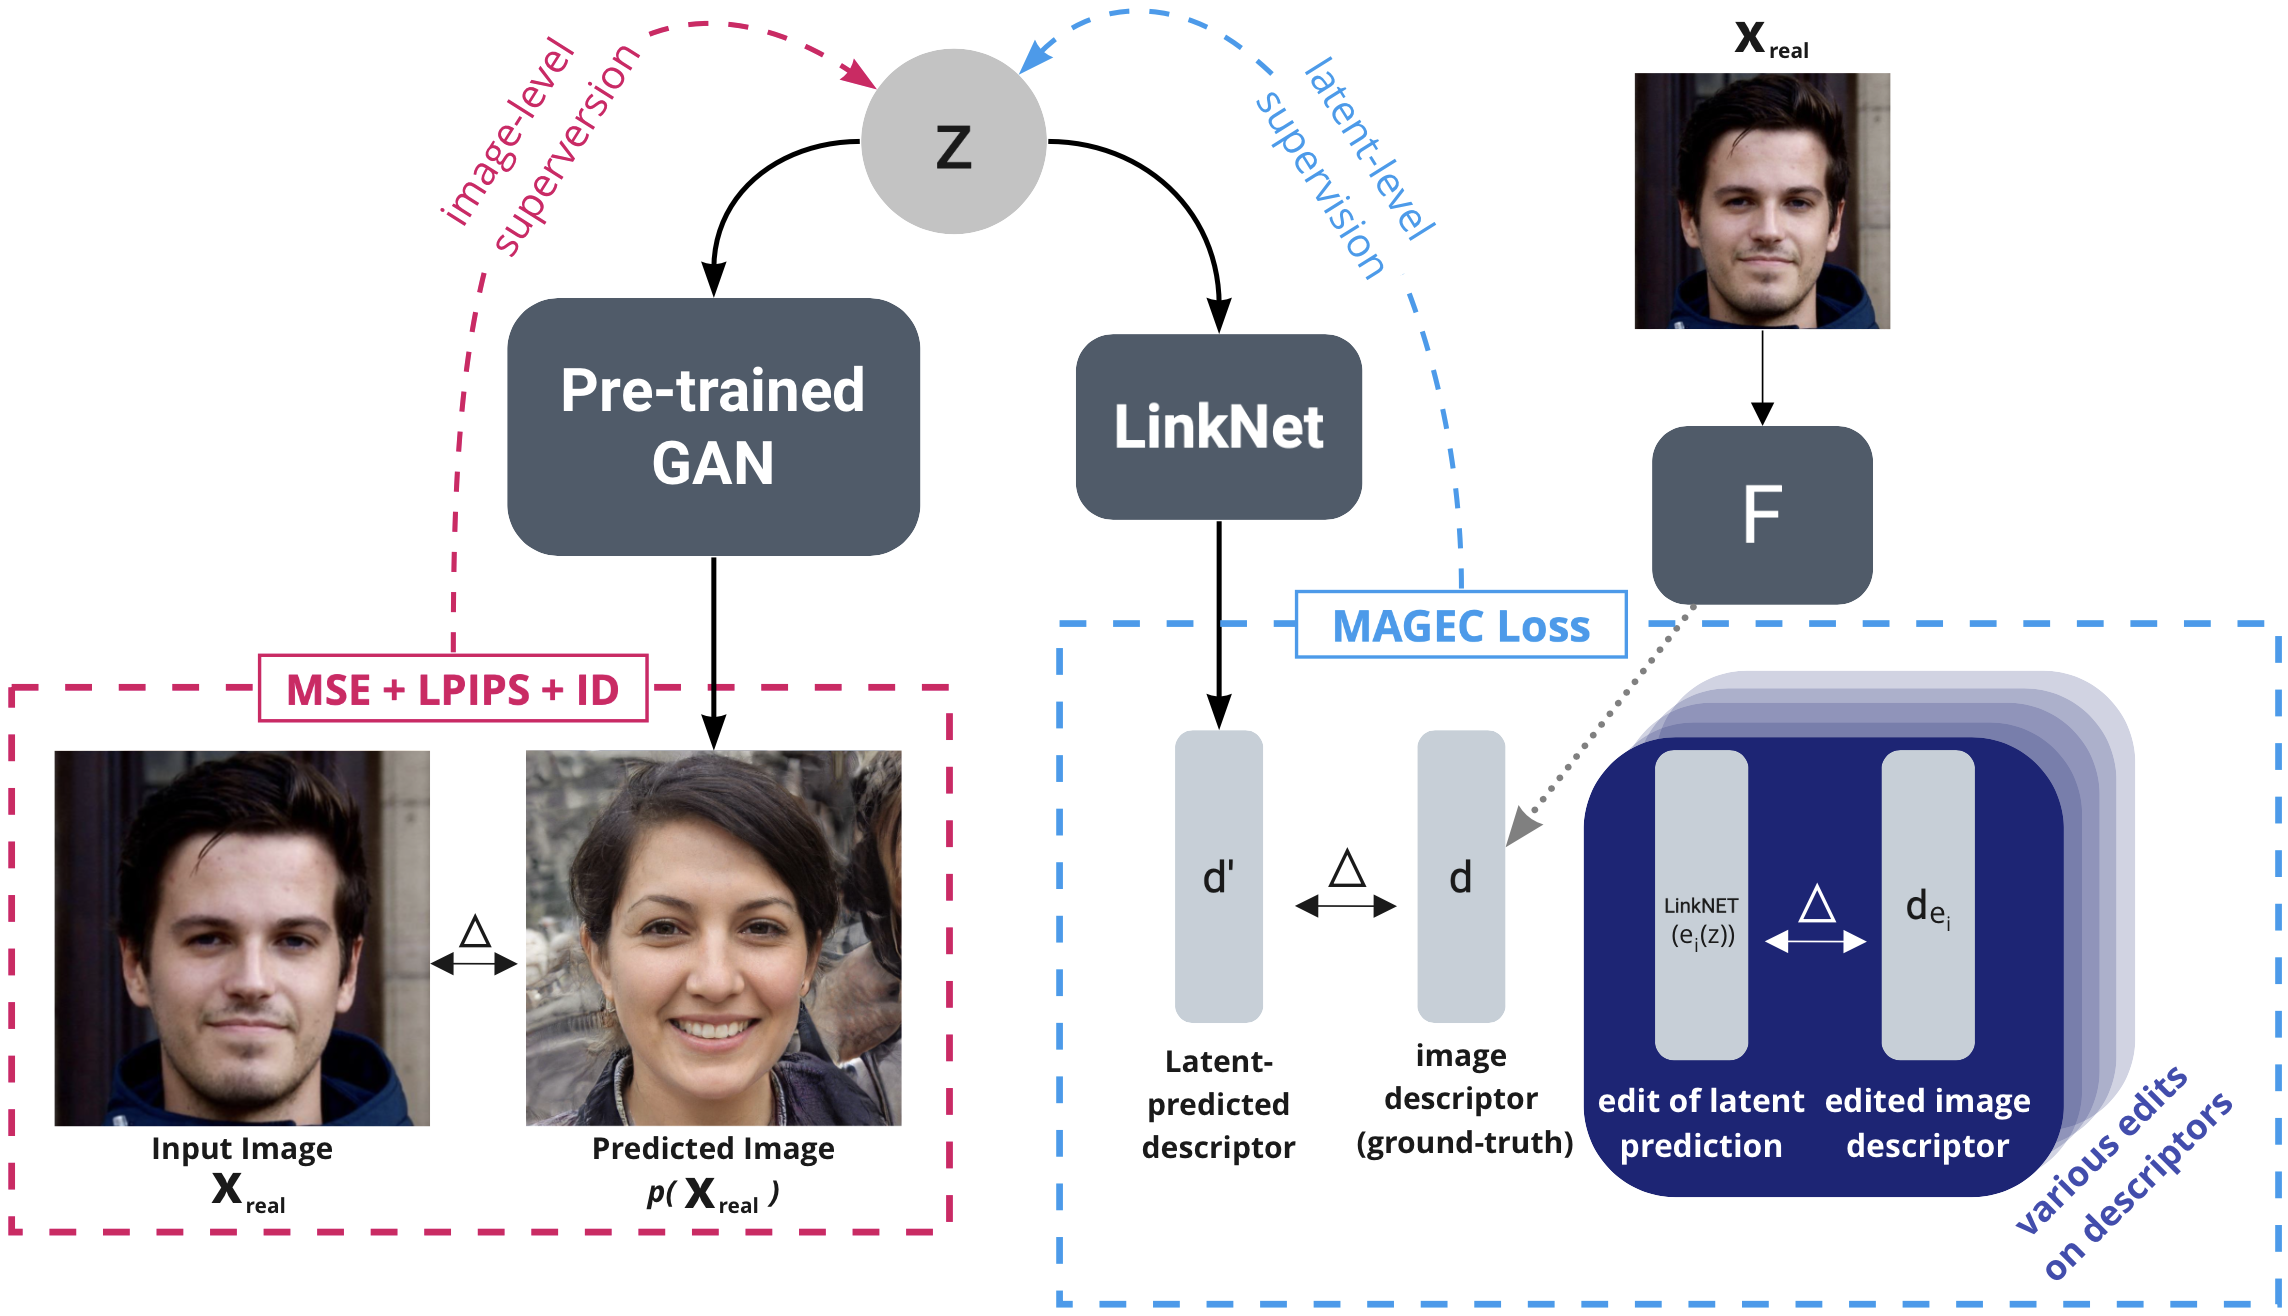
\includegraphics[width=\textwidth]{images/magec/training_protocol9.png}
    \caption{Our proposed optimization framework. We initialize our $\z$ vector with $\z_0$. Then, we generate the associated image with the pre-trained generator to obtain the image-level loss. We predict the latent-level descriptor $d'$ with our pre-trained $\linknet$. We add a consistency loss of these features with the ``ground-truth'' features $d$ evaluated from our feature-extractor network $F$. We add another consistency loss over the edited descriptors (using a differentiable editor $e$) and the ``ground-truth'' edits which we obtain by modifying $d$. This MAGEC loss gives us latent-level optimization which promotes editability and an in-domain output vector.}
    \label{fig:training_protocol}
\end{figure*}


\subsection{MAGEC Loss}
Now that we have linked our image and latent space with the simple $\linknet$,
 we can define our i\textbf{MAG}e-lat\textbf{E}nt \textbf{C}onsistency ``\magec''
  loss in the following way, built from Eq.\ref{classic_inversion_with_perceptual}. 

First, we add an image-latent consistency loss over the input image and the 
latent to optimize. We obtain the ``ground-truth'' image descriptor $d$ using $F$, 
then we use our $\linknet$ to predict the image descriptor $d'$ from latent vector
 $\z$. If the latent vector correctly represents the image, it should be able to 
 predict the associated image predictors.


Second, we add an image-latent edit consistency loss. Let $e$ be a differentiable 
known editor with $i$ editing operations (for example, an editing operation can 
be \emph{add glasses}, \emph{remove wrinkles}, \emph{to woman}, etc.). We
 perform $i$ edits of the latent vector $e_i(\z)$ and edit the 
 ``ground-truth'' image descriptor $d$ accordingly to obtain
  $d_{e_i}$. Our edited latent vector should be able to predict $d_{e_i}$
   (with $\linknet$). See Fig.~\ref{fig:training_protocol} for detailed
    illustration.

The \magec loss is given as follows:

\begin{equation}\label{MAGEC}
    \mathcal{L}_{\text{MAGEC}}(\z, \x_{real}) = \underbrace{\mathcal{L}_F(\linknet(\z), d)}_{\text{image-latent consistency  %\\ between the input image and predicted latent
    }} 
    + 
    \underbrace{\frac{1}{|edits|} \sum_{i \in edits}{\mathcal{L}_F(\linknet(e_i(\z)), d_{e_i})}}_{\text{image-latent edit consistency %of the input image\\ and the corresponding edits of the predicted latent.
    }}
\end{equation}

where $d = F(\x_{real})$ and $d_{e_i}$ is the modified $d$ according to edit $i$.

Our final loss is

\begin{equation}\label{final_loss_term} \begin{split}
\mathcal{L}(\z, \x_{real}) &= \lambda_{\text{MSE}}\mathcal{L}_2(G(\z), \x_{real}) + \lambda_{\text{LPIPS}}\mathcal{L}_{\text{LPIPS}}(G(\z), \x_{real}) \\&+ \lambda_{\text{ID}}\mathcal{L}_{\text{ID}}(G(\z), \x_{real}) +  \lambda_{\text{MAGEC}}\mathcal{L}_{\text{MAGEC}}(\z, \x_{real})
\end{split} \end{equation}


\noindent where $\mathcal{L}_{\text{ID}}$ is the \emph{ID loss} introduced
 in  \cite{psp, e4e}
 based on a pre-trained ArcFace \citep{deng2018arcface} network 
 (or ResNet50 \citep{he2016resnet} network trained with MOCOv2  
 \citep{mocov2_paper} for non-face images), and $\mathcal{L}_{F}$ was the loss 
 used to train the feature extractor $F$.

As we can see in Fig.~\ref{fig:training_protocol}, our framework allows dual 
supervision, simultaneously in the image and latent spaces. We are able to
 provide latent editing directly in the loss term, which not only allows to 
 generate editable latents, but also helps to visualize which images are 
 inherently out-of-domain for the GAN in question. Moreover, this framework 
 can be incorporated into any pre-trained GAN, and allows potential further 
 constraint by combining several differentiable editing methods together.

\section{Experimental Setup}

We propose to evaluate our \magec strategy on two benchmarks typically 
used to evaluate \ac{GAN}s - Faces and Cars. 

\subsection{Experimental Setup for Face edits}

\minipar{Datasets and Evaluation editors}

We perform thorough evaluation of our method using 1000 random samples from the CelebAHQ 
\citep{karras2018progressive} dataset. We evaluate our projection on four well-known editing methods: InterfaceGAN 
 \citep{shen2020}, GANSpace \citep{harkonen2020ganspace}, StyleFlow \citep{abdal2020styleflow} and random 
 interpolation between latent vectors \citep{karra2019stylegan}.

 \minipar{Pretrained GAN Model}
 We use StyleGAN2, pre-trained on FFHQ for $1024 \times 1024$ output resolution as our
 pre-trained GAN. We use the mapped latent space $\mathcal{W}$ and similarly to 
  \citep{abdal2019image2stylegan, abdal2020, psp, zhu2020indomain, e4e}, we extend this
   space to $\mathcal{W+}$ by allowing each of the $512$-dimensional \emph{style vectors}
    to be independent of each other. 

\minipar{Training Configurations}

For the feature extractor $F$, we train an attribute-classifier
on CelebA \citep{celeba} to predict 40 binary attributes. We use a 
ResNet50 backbone \citep{he2016resnet}
and ajust the dimensions of the last fully-connected layer to 40. We finetuned 
this model by first 
training the last layer for 2 epochs with a learning rate of 0.02 and then 
finetuning 
the entire model with discriminative learning rates ranging from 0.002 to
 0.02, as described 
in \cite{howard2018universal}.
    
To train our $\linknet$ model,
we sample $50,000$ (latent, descriptor) training pairs with our pre-trianed StyleGAN2. 
Note that we use the extended $\mathcal{W+}$ space for generation, meaning 
that we generate a distinct latent vector for each style block of StyleGAN2. 
We use the predicted binary labels of $F$ as our ground-truth labels for the 
$\linknet$ training.
    
For our $\linknet$ model, we use a sigmoid activation function and 
binary cross-entropy 
loss. We use 
the Adam \citep{adam} optimizer with the default parameters. We 
trained the model for $10$ epochs and evaluated on a separate validation set, 
achieving a 
$89\%$ accuracy.
    
    
Finally, we use InterfaceGAN 
\citep{shen2020} as our editor $e$ to supervise our \magec loss, 
which performs 
add/remove operations on all 40 attributes. 


\minipar{Optimization Protocol} 
We initialize $\z$ with $\z_{avg}$, by sampling 
$N = 50000$ latent vectors with StyleGAN2 and taking the average vector $\z_0 = \z_{avg}$. 
Fig.\ref{fig:avg_ffhq} shows the generated output of the average latent vector.
We use the Adam optimizer \citep{adam} with the default parameters 
($\beta_1=0.9$, $\beta_2=0.999$, $\epsilon=1e^{-08}$). We perform our training in two
 parts. First,
we use $\lambda_{\text{MAGEC}} = 3e^{-4}$, $\lambda_{\text{LPIPS}} = 5e^{-1}$, 
$\lambda_{\text{MSE}} = 1e^{-3}$ and $\lambda_{\text{ID}} = 3e^{-4}$ and perform 100 
optimization
 steps. Then, we set $\lambda_{\text{MSE}} =  \lambda_{\text{LPIPS}} = 5e^{-1}$ for another 
 100 
 optimization steps, leaving the other loss coefficients unchanged. The learning rate 
 begins at $0.07$ and is exponentially decayed with a decay factor of $0.8$ every 
 $25$ epochs. Our two-steps procedure is motivated by the fact that 
 instance-based optimization often fails at adding semantic information
  in the 
 latent vector with small optimization steps. When placing a higher weight 
 on
  $\lambda_{\text{MAGEC}}$, we direct our latent vector $\z$ to a strong point which 
  captures 
  this semantic information. Once the latent vector is within the correct 
  ``area'' of 
  the latent space, we can give more relative weight to the loss coefficients 
  related 
  to image reconstruction.



 \subsection{Experimental Setup for Car edits}

 \minipar{Datasets and Evaluation Editors}
 We evaluate  our method using random 
 images from the Stanford Cars test set \citep{stanford_cars}, not 
 used to train $F$ (detailed below). We use the GANSpace 
 \citep{harkonen2020ganspace}
  editing method to evaluate editability.

\minipar{Pretrained GAN Model}
We use StyleGAN2, pre-trained on LSUN Cars for $384 \times 512$ output resolution
as our
pre-trained GAN. We use the mapped latent space $\mathcal{W}$ and as before,
we extend this
space to $\mathcal{W+}$ by allowing each of the $512$-dimensional \emph{style vectors}
  to be independent of each other. 


\minipar{Training Configurations} 
For our feature extractor $F$, we use a pre-trained publically available\footnote{https://github.com/sigopt/stanford-car-classification} cars 
classifier \citep{pretrained_cars} which classifies the image 
into one of $196$ car models.

Since the ``average''
latent vector from the pre-trained \emph{cars} StyleGAN2 is a 
poor representation of a car
(see Fig.~\ref{fig:avg_cars}), we train an encoder 
$E$ which predicts a latent vector from an image. This was 
used to initialize the latent vector for further optimization.
We used a pre-trained ResNet50 model \citep{he2016resnet} 
as our backbone, and modified the last layers to output
a latent vector. Generated data was used for training.


We follow the same training for the $\linknet$ as before, except we use a 
softmax activation function to predict the car model, and use the 
predicted binary label from $F$ as our ground-truth label to supervise 
training. We achieve a $95\%$
accuracy on our validation set. It should be noted however, that our ground-truth 
   car predictor often classified the generated cars in the same class 
   due to high discrepancy
    between real and generated cars (generated cars generally
     don't have distinctive logos).

 Finally, we use GANSpace 
 \citep{harkonen2020ganspace} as our editor $e$ to supervise our \magec loss. 
 It's worth noting
that GANSpace does not allow edits of the car model, so our
\magec loss supervises our training in a weaker fashion than 
 before. Here, the modified ``ground-truth'' feature vector is 
 simply the image descriptor vector, since the car model should 
 not change with GANSpace edits.


\noindent \textbf{Optimization Protocol}  We initialize $\z$ with
 $\z_0 = E(\x_{real})$. Training is again effectuated in two parts.
  First, we optimize for $50$ steps using 
  $\lambda_{\text{MAGEC}}=5e^{-2}$ and $\lambda_{\text{MSE}} = \lambda_{\text{LPIPS}} = 5e^{-1}$ 
  with a learning rate of $0.08$. Then, we decrease 
  $\lambda_{\text{MAGEC}}=5e^{-8}$ with a learning rate of $0.01$ and 
  train for $50$ more steps. We use the Adam optimizer \citep{adam}
  with default parameters for  
  the training.



\subsection{Baselines}
We compare our method with Image2StyleGAN++ \citep{abdal2020}, the state-of-the-art
 optimization-based method for GAN-Inversion. This method uses the classic loss from
  Eq.~\ref{classic_inversion_with_perceptual} (using the LPIPS \citep{zhanglpips2018} loss 
  as the perceptual loss) and first optimizes the latent vector for 1000 iterations, then
   the noise vector for 1000 iterations. This loss can be seen as an ablation of the \magec 
   and ID losses from Eq.~\ref{final_loss_term}, but minimized over more iterations. We
    also perform an ablation study using our training protocol to optimize 
    Eq.~\ref{final_loss_term} but without the \magec loss. We initialize the starting 
    vector $\z_0$ for all methods 
    in the same way as us.


\begin{figure*}
  \centering
    \includegraphics[width=\textwidth]{images/magec/im2st_comparison.png}
    \caption{Comparison of our method vs Im2StyleGAN++. Left: original images. Top rows: 
    Im2StyleGAN++ projection. Bottom rows: Our projection with \magec. Edits are made 
    using GANSpace. While Im2StyleGAN++'s projection is accurate, edits present strong 
    artifacts or absurdities. Our reconstructions are also accurate, but react correctly 
    to editing operations, suggesting that it follows the native distribution of StyleGAN
     more closely.}
    \label{fig:im2stcomparison}
\end{figure*}


\begin{figure*}
  \centering
  \begin{subfigure}[b]{0.45\textwidth}
      \centering
      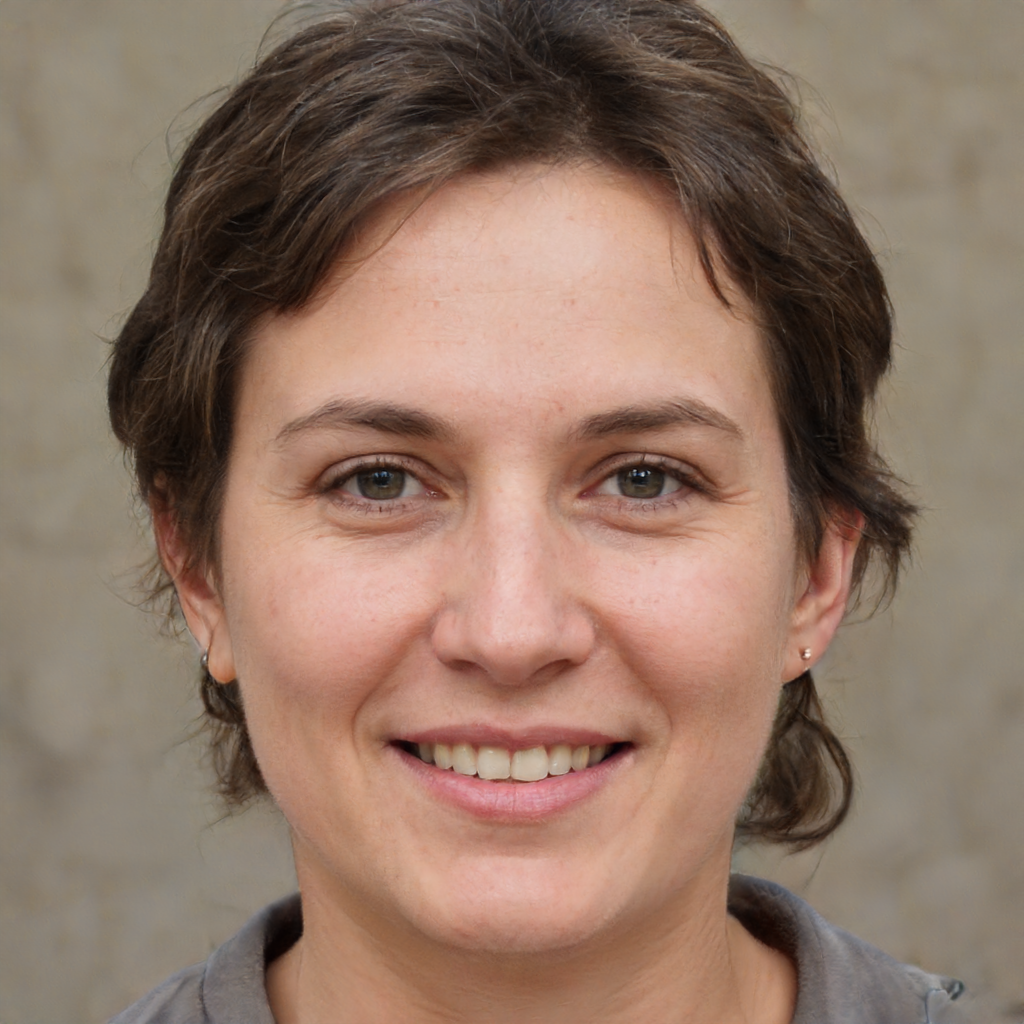
\includegraphics[width=\textwidth]{images/magec/face_average.png}
      \caption{Average latent vector from the pre-trained StyleGAN2 on FFHQ.}
      \label{fig:avg_ffhq}
  \end{subfigure}
  \hfill
  \begin{subfigure}[b]{0.45\textwidth}
      \centering
      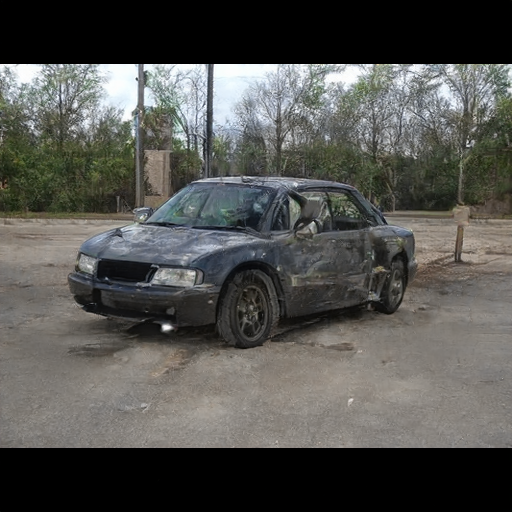
\includegraphics[width=\textwidth]{images/magec/car_average.png}
      \caption{Average latent vector from the pre-trained StyleGAN2 on LSUN cars.}
      \label{fig:avg_cars}
  \end{subfigure}
  \caption{Average latent vectors from two different pre-trained StyleGANs}
  \label{fig:stylegan_averages}'
\end{figure*}



%\subsection{Results}

\section{Qualitative Results} 
Fig.~\ref{fig:teaser} shows our method and various 
edits applied on notorious figures. As we can see in Fig.~\ref{fig:im2stcomparison}, 
our method is visually  superior to Im2StyleGAN \citep{abdal2020} in terms of 
editing quality. While \cite{abdal2020} produces artifacts and blur during edits, our
 method produces sharp, realistic edits.

 \begin{figure*}
  \centering
    \includegraphics[width=\textwidth]{images/magec/teaser2.png}
    \caption{From left to right: original image, projection in latent space using \magec loss, various edits (GANSpace, InterfaceGAN and StyleFlow respectively). Edits are of high-quality, and conform to expectations of the various editing methods. Best viewed zoomed.}
    \label{fig:teaser}
\end{figure*}
 


In terms of assessing visual quality, human evaluation is still
 the gold standard \citep{hype, e4e}. We have thus provided 
 abundant uncurated visual results using our method and comparing
  it to Image2StyleGAN++ \citep{abdal2020} as well as to our 
  ablated method without the \magec loss. 
Fig.~\ref{fig:interfacegan_supp},~\ref{fig:styleflow_supp}, 
~\ref{fig:ganspace_sup}, and ~\ref{fig:interpol_sup} show examples with the 
respective four editing methods: InterfaceGAN \citep{shen2020}, StyleFlow
 \citep{abdal2020styleflow}, GANSpace \citep{harkonen2020ganspace}, and 
 random interpolations \citep{karra2019stylegan}. When viewing the results, 
 take extra care to notice the reconstructions (compared to the original images) as 
 well as the result of the intended edit operation (with respect to the original 
 image). Figures should ideally be viewed zoomed and in color. Note that ambiguous
  edit operations like  \emph{gender}, \emph{expression} and \emph{age} should flip
   the attribute in question (for example, \emph{age} edit means young turns to old,
    and vice versa).  The following general observations can be made:

\begin{itemize}
    \item Image2StyleGAN++ \citep{abdal2020} produces very accurate reconstructions, but edits are often of abysmal quality.
    \item Ablating the \magec loss leads to worse reconstructions.
    \item Ablating the \magec loss produces edits that are of good-quality, but often don't respect the edit intention (for example, the \emph{glasses} edit may not make any noticeable change, despite producing a high-quality image) nor fidelity to the input image.
    \item Our \magec loss gives accurate reconstructions, but also produces the intended edits that are sharper, less noisy, and of higher-quality.
\end{itemize}




Finally, we applied our method onto images of real cars. Visual results 
can also be seen in the end of this chapter in Fig.~\ref{fig:cars}. As expected, 
Image2StyleGAN++'s projection leads to distorted and inaccurate 
edits. When comparing our method to the ablated method, we can 
see that \magec helps editing and reconstruction. Notice the 
rotation operations for the first and second cars in 
Fig.~\ref{fig:cars}. The red car preserved the ``sports car'' 
look while the white car similarly preserved the \emph{Audi} 
logo .  Finally, the last rows show that we were correctly able 
to reconstruct the \emph{BMW} model as well as preserving it 
during edits.

We used a very general pre-trained classifier $F$ which was 
rather unrelated to the edits of the GANSpace editor that 
supervised our training. Moreover, our method assumes that 
StyleGAN's latent code can predict the specific car model, a 
strong assumption, especially considering that purely generated 
car images rarely have a clear logo. It is more likely that the 
latent code encodes some sort of ``shape'' which roughly predicts
 the car model with $\linknet$. Despite these limits, we can see that
  adding this simple \magec loss using an arbitrary auxiliary 
  classifier does indeed improve editing and reconstruction 
  capacity for many cases, giving high promise to the capacity and
   flexibility of our method.




   \begin{figure*}
    \centering
      \includegraphics[width=0.93\textwidth]{images/magec/interfacegan_large.jpeg}
      \caption{InterfaceGAN \citep{shen2020} edits using various inversion methods.  Our method gives the intended edits with high-quality results. Best viewed zoomed and in color.}
      \label{fig:interfacegan_supp}
  \end{figure*}
  
  \begin{figure*}
    \centering
      \includegraphics[width=\textwidth]{images/magec/styleflow_large.jpeg}
      \caption{StyleFlow \citep{abdal2020styleflow} edits using various inversion methods. Remark that here, the edits should be \textbf{cumulative}. Our \magec loss helps to produce accurate reconstructions as well as the intended edits with high-quality results.}
      \label{fig:styleflow_supp}
  \end{figure*}
  
  \begin{figure*}
    \centering
      \includegraphics[width=\textwidth]{images/magec/ganspace_large.jpeg}
      \caption{GANSpace \citep{harkonen2020ganspace} edits using various inversion methods. Image2StyleGAN++'s inversion method produces accurate reconstructions, but distorted and low-quality edits. Using our \magec loss greatly helps with reconstruction, but also helps to produce the intended change (notice \emph{male} / \emph{female} edits in particular). Best viewed zoomed and in color.}
      \label{fig:ganspace_sup}
  \end{figure*}
  
  \begin{figure*}
    \centering
      \includegraphics[width=\textwidth]{images/magec/interpol_large.jpeg}
      \caption{Interpolations \citep{karra2019stylegan} using various inversions. Take extra notice of the reconstructions, where our \magec loss clearly helps. In the first edit, only our edit gives a beard which clearly progressively disappears (rather than increasing then decreasing), suggesting stronger semantic information in the inverted latent. In the last case, notice the gradual background changes in the third set with our method, compared to the harsher change of Im2StyleGAN++'s edit.  Best viewed zoomed and in color.}
      \label{fig:interpol_sup}
  \end{figure*}
  
  \begin{figure*}
    \centering
      \includegraphics[width=0.835\textwidth ]{images/magec/cars_super_large.pdf}
      \caption{GANSpace \citep{harkonen2020ganspace} edits with various inversions. Image2StyleGAN++'s method produces good reconstructions but distorted edits. Our method helps in preserving the car model during reconstruction and edits. Remark the top red car when rotated: our method preserves the \emph{sports car} style. Remark that the \emph{Audi} logo of the white car is also conserved when rotating. Finally, the bottom red car reveals that our method consistently maintains the correct car model (\emph{BMW}) during reconstruction and edits. Best viewed zoomed and in color.}
      \label{fig:cars}
  \end{figure*}

\section{Quantitative Evaluation} 

\subsection{Reconstruction and Editability}

Tab.~\ref{tab:reconstruction_results} shows the various
 metrics for reconstruction. Notice that adding our \magec loss in Eq.~\ref{final_loss_term} leads a better reconstruction. Even when allowing 50\% more iterations, our method still performs on par in terms of reconstruction. The \magec loss could thus be seen as a prior which speeds up optimization. As expected, \cite{abdal2020} performs excellent reconstruction, given the time (over 4 minutes) and the under-constrained loss function.

% 11041917

\begin{table}[]
\begin{tabular}{|l|l|l|l|l|}
\hline
{  }                             & {  MSE $\downarrow$}    & {  LPIPS $\downarrow$} & {  Nb opt. steps $\downarrow$} & {  Time (s) $\downarrow$} \\ \hline
{  Full Method}                  & {  0.0040} & {  0.053} & {  200}           & {  34.6}     \\ \hline
{  w/o \magec}                    & {  0.0094} & {  0.062} & {  200}           & {  29.7}     \\ \hline
{  w/o \magec + extra opt. steps} & {  0.0078} & {  0.050} & {  300}           & {  44.5}     \\ \hline
{  Im2StyleGAN++}                  & {  0.0012} & {  0.018} & {  2000}          & {  242.2}    \\ \hline
\end{tabular}\caption{Reconstruction evaluation of projection, showing averages per image. We should note that the time of our method directly depends on the number of attributes we add to our \magec loss (Eq.~\ref{MAGEC}). Here, adding editing constraints for 40 attributes leads to a cost of about 5 seconds per image.}\label{tab:reconstruction_results}
\end{table}


We perform random edits on the 1000 images to obtain 20000 edited images per projection 
method. The semantic editability of the inverted latent vector is of utmost importance 
when performing GAN Inversion, but there is no standard metric for measuring this. We 
first evaluate using common metrics before introducing our novel ``editability score''.

We aim to evaluate the realism and ``coherence'' of a given edit. The FID score 
\citep{fidscore} is not adapted to measure the quality of the edits, firstly because the 
original sample size (1000 original images) is well-below the recommended 50,000 needed 
for an accurate FID score, and secondly because our edits inherently lack diversity 
(edits of the same image resemble each other).
Instead, we use the \emph{realism score} \citep{precision_recall}, which evaluates an 
image instead of a distribution. This is a nearest-neighbor based method 
(higher is better) in which the \emph{realism threshold} is set to $1$ (a score above 
$1$ is a realistic image). 

To measure the ``coherence'' of an edit, we calculate a simple ``improved-target'' score
 $t$ to measure the net difference of the predicted attribute probability before and 
 after the attribute-targeted edit by using a pre-trained attribute classifier. A higher
  value means that the attribute prediction increased after applying the editing method,
   meaning it reacted accordingly. Note that $t \in [0, 1]$. Remark that this metric is 
   only applicable to the editors which make attribute-specific edits (InterfaceGAN 
   \citep{shen2020} and StyleFlow \citep{abdal2020styleflow}).

For reliable interpretation of these metrics, we performed a paired Student's t-test on 
our method and a competing method, as the edit operations were the same for all projected
 images. Our results are summarized in Tab.~\ref{tab:standard_metrics}. As we can see, 
 our method performs well on these metrics, always among the best in terms of realism or 
 ``coherence". However, these results are not entirely conclusive, and we investigate a 
 better metric in order to evaluate the editability of a given inversion.

% \begin{table}[]
% \begin{tabular}{lcccccc}
% \hline
% \multicolumn{1}{|l|}{}               & \multicolumn{2}{c|}{InterfaceGAN}                                                      & \multicolumn{2}{c|}{StyleFlow}                                                         & \multicolumn{1}{c|}{GANSpace}         & \multicolumn{1}{c|}{Interpolations} \\ \hline
% \multicolumn{1}{|l|}{}               & \multicolumn{1}{c|}{\textit{realism $\uparrow$}} & \multicolumn{1}{c|}{\textit{t $\uparrow$}} & \multicolumn{1}{c|}{\textit{realism $\uparrow$}} & \multicolumn{1}{l|}{\textit{t $\uparrow$}} & \multicolumn{1}{c|}{\textit{realism $\uparrow$}} & \multicolumn{1}{c|}{\textit{realism $\uparrow$}}      \\ \hline
% \multicolumn{1}{|l|}{Im2StyleGAN++ \cite{abdal2020}} & \multicolumn{1}{c|}{0.99}          & \multicolumn{1}{c|}{0.08}                    & \multicolumn{1}{c|}{0.98}          & \multicolumn{1}{c|}{0.19}                   & \multicolumn{1}{c|}{0.97}          & \multicolumn{1}{c|}{0.99}               \\ \hline
% \multicolumn{1}{|l|}{w/o MAGEC}      & \multicolumn{1}{c|}{\textbf{1.01}}          & \multicolumn{1}{c|}{0.09}                    & \multicolumn{1}{c|}{\textbf{0.99}} & \multicolumn{1}{c|}{0.15}                   & \multicolumn{1}{c|}{\textbf{0.99}} & \multicolumn{1}{c|}{0.99}               \\ \hline
% \multicolumn{1}{|l|}{Full Method}    & \multicolumn{1}{c|}{\textbf{1.01}} & \multicolumn{1}{c|}{\textbf{0.10}}           & \multicolumn{1}{c|}{\textbf{0.99}}          & \multicolumn{1}{c|}{\textbf{0.20}}          & \multicolumn{1}{c|}{\textbf{0.99}} & \multicolumn{1}{c|}{\textbf{1.05}}      \\ \hline
%                                      & \multicolumn{1}{l}{}                  & \multicolumn{1}{l}{}                           & \multicolumn{1}{l}{}                  & \multicolumn{1}{l}{}                           & \multicolumn{1}{l}{}                  & \multicolumn{1}{l}{}                      
% \end{tabular}\caption{Evaluation of random edits with \emph{realism scores} and an ``improved targets'' score by using a pre-trained classifier. While these results along are not conclusive, our method still responds well to edits and produce realistic edits according to the \emph{realism score}.}\label{tab:standard_metrics}
% \end{table}

% \usepackage{arydshln}


\begin{table}
\centering
\begin{tabular}{|l|c|c|c|c|c|c|}
\hline
               & \multicolumn{2}{c|}{ InterfaceGAN} & \multicolumn{2}{c|}{ StyleFlow} &  GANSpace &  Interpolations \\ \hline
               &  \textit{realism}      &  \textit{t}         &  \textit{realism}    &  \textit{t}        &  \textit{realism}  &  \textit{realism}        \\ \hline
 Im2StyleGAN++  &  0.973                 &  0.096     &  0.929               &  \textbf{0.211}    &  0.960             &  1.00           \\ \hline
 w/o MAGEC loss &  \textbf{0.994}        &  0.097              &  \textbf{0.976}      &  0.148             &  \textbf{0.985}    &  1.03                    \\ \hline
 Full Method    &  \textbf{0.998}        &  \textbf{0.122}     &  \textbf{0.982}      &  \textbf{0.202}    &  \textbf{0.984}    &  \textbf{1.04}           \\ \hline
\end{tabular}\caption{ \emph{Realism scores} and ``improved target'' scores of random image edits. For reliable interpretation, we perform a paired Student's t-test between our method's metrics and the competing method. The bold values are in line with this significance (\emph{p}-value $< 0.05$). Our method consistently produces realistic and coherent images for the task at hand.}\label{tab:standard_metrics}
\end{table}




\subsection{Edit-Consistency Score}

The standard metrics at evaluating image quality are poorly adapted to evaluating a 
projection. Firstly, as we saw in the previous section, reconstruction and editability 
metrics are independent, which makes it difficult to choose a good trade-off without an 
ad hoc solution. Moreoever, the standard image quality metrics presented in Tab. \ref{tab:standard_metrics}
have no way of evaluating whether or the edited image is coherent with regards to the input image. 
We aim to address both of these weaknesses with a custom metric, the \emph{edit-consistency score}.
 
 We first use 
our projection method $p$ to obtain vector $\z$ from $\x_{real}$. Then, we use a known 
editing method $e$ to edit the vector with respect to a certain attribute, giving us
 $\x_{edit}$. Then, we re-project it into the latent space to obtain $\z'_{edit}$. Finally,
  we apply the inverse editing method onto $\z'_{edit}$ to obtain a cyclic image 
  $\x_{cyc}$, which should ideally match the initial projection.
  Fig.~\ref{fig:ecs_intuition} shows an overview of how we calculate this score.
  
  We define the 
  edit-consistency loss as follows:

\begin{equation}
    ecs(p, \x_{real}) = \frac{2 \times \mathcal{L}_{\text{LPIPS}}(p(\x_{real}), \x_{cyc})}{\mathcal{L}_{\text{LPIPS}}(p(\x_{real}), \x_{edit}) + \mathcal{L}_{\text{LPIPS}}(\x_{edit}, \x_{cyc})}
\end{equation}


\noindent The intuition is that the cyclic image should resemble the projected image, but
 images should also react accordingly to editing methods.
Remark that a ``perfect'' $ecs$ score is $0$. An $ecs$ of $1$ can be seen as a 
``quality'' threshold, since $ecs > 1$ means that the distance
 $\mathcal{L}_{LPIPS}(p(\x_{real}), \x_{cyc})$ is larger than one of the two edit
  operations.
 See Fig.~\ref{fig:ecs_examples} for examples of varying $ecs$ scores. We can now define 
 the edit-consistency score of a projection :
  \begin{equation} ECS(p) = \frac{1}{|X|}\sum_{\x_{real} \in X}{ecs(p, \x_{real})}. \end{equation}


\begin{table}
    \centering
\begin{tabular}{|l|l|l|l|l|}
\hline
              & \multicolumn{2}{c|}{ InterfaceGAN}             & \multicolumn{2}{c|}{ GANSpace}                          \\ \hline
              &   \textit{Male} $\downarrow$ &   \textit{Smile} $\downarrow$ &   \textit{Male} $\downarrow$ &   \textit{Smile} $\downarrow$ \\ \hline
  Im2StyleGAN++ &   0.97     &   1.00               &   1.07              &   0.98               \\ \hline
  w/o \magec     &   1.01             &   0.95                       &   1.06                      &   0.90                       \\ \hline
  Full Method   &   \textbf{0.84}             &   \textbf{0.87}                       &   \textbf{0.95}                      &   \textbf{0.79}                       \\ \hline
\end{tabular}
\caption{$ECS$ evaluation. Our \magec loss significantly improves $ECS$ for all edits, notably ones not used to supervise our loss (GANSpace). Scores are evaluated on images not containing the target attribute.}\label{tab:ECSes}
\end{table}


Tab.~\ref{tab:ECSes} compares $ECS$ results between our method and the two baselines. 
Importantly, notice how our method gives better scores for an editing method not utilized 
to supervise the loss (GANSpace), suggesting that the latent vector doesn't overfit to
 one editing method, but is encouraged to become ``in-domain''.

\subsection{Human Evaluation}

While automatic quantitative methods allow quick 
comparisons to baseline methods, many have observed \citep{hype} that human judgment is 
still the most reliable metric for evaluating image quality. We thus performed a user 
study in which experts of photography were asked to judge photo edits between each other,
 each one corresponding to a different projection method. See Fig.\ref{fig:user_interface}
 which shows the user interface to rate edits.
 One of the two edits were our 
 method, while the other one was either produced by our  ablated method 
 (Eq.~\ref{final_loss_term} without the \magec loss) or by Im2StyleGAN++ \citep{abdal2020}.
 Each edit operation consisted in changing one of 10 possible facial attributes
 to a random new value, using either GANSpace \citep{harkonen2020ganspace} or 
 StyleFlow \citep{abdal2020styleflow}. For fairness, InterfaceGAN \citep{shen2020} was not included 
 in the edits, as this method was used to supervise our loss. When an expert judged an edit, 
 a new proposition appeared immediately after and the survey automatically stopped after 5 minutes 
 to ensure high-quality responses. In total, about 30 responses were collected from each expert. 
Tab. \ref{tab:userstudyresults} shows the results. As we can see, the experts had a 
strong preference for our method.
 
 

 \begin{figure*}
  \centering
  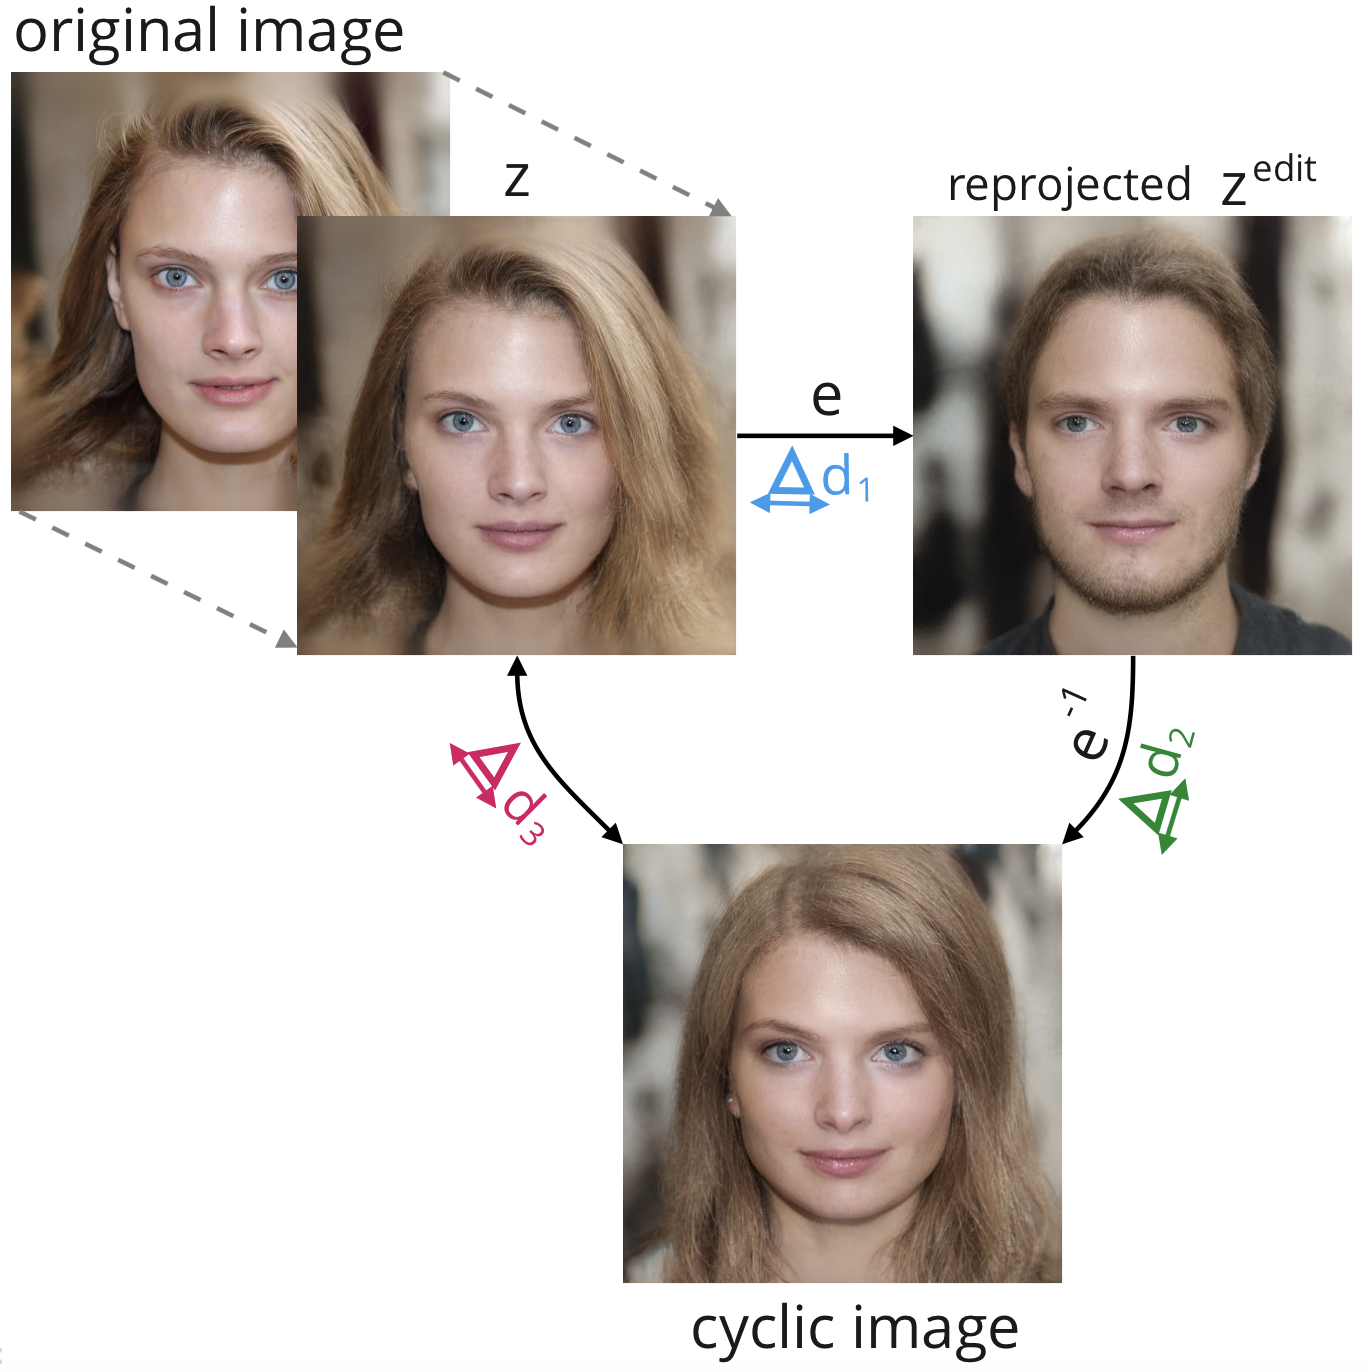
\includegraphics[width=0.8\textwidth]{images/magec/edit_consistency5.png}
  \caption{Calculating $ecs$. We perform 2 projections per $ecs$: 1 from the original image, and one from the edited latent. A better (lower) $ecs$ means that $d_3$ is smaller than $d_1$ and $d_2$}
  \label{fig:ecs_intuition}
 \end{figure*}


\begin{figure*}
  \centering
  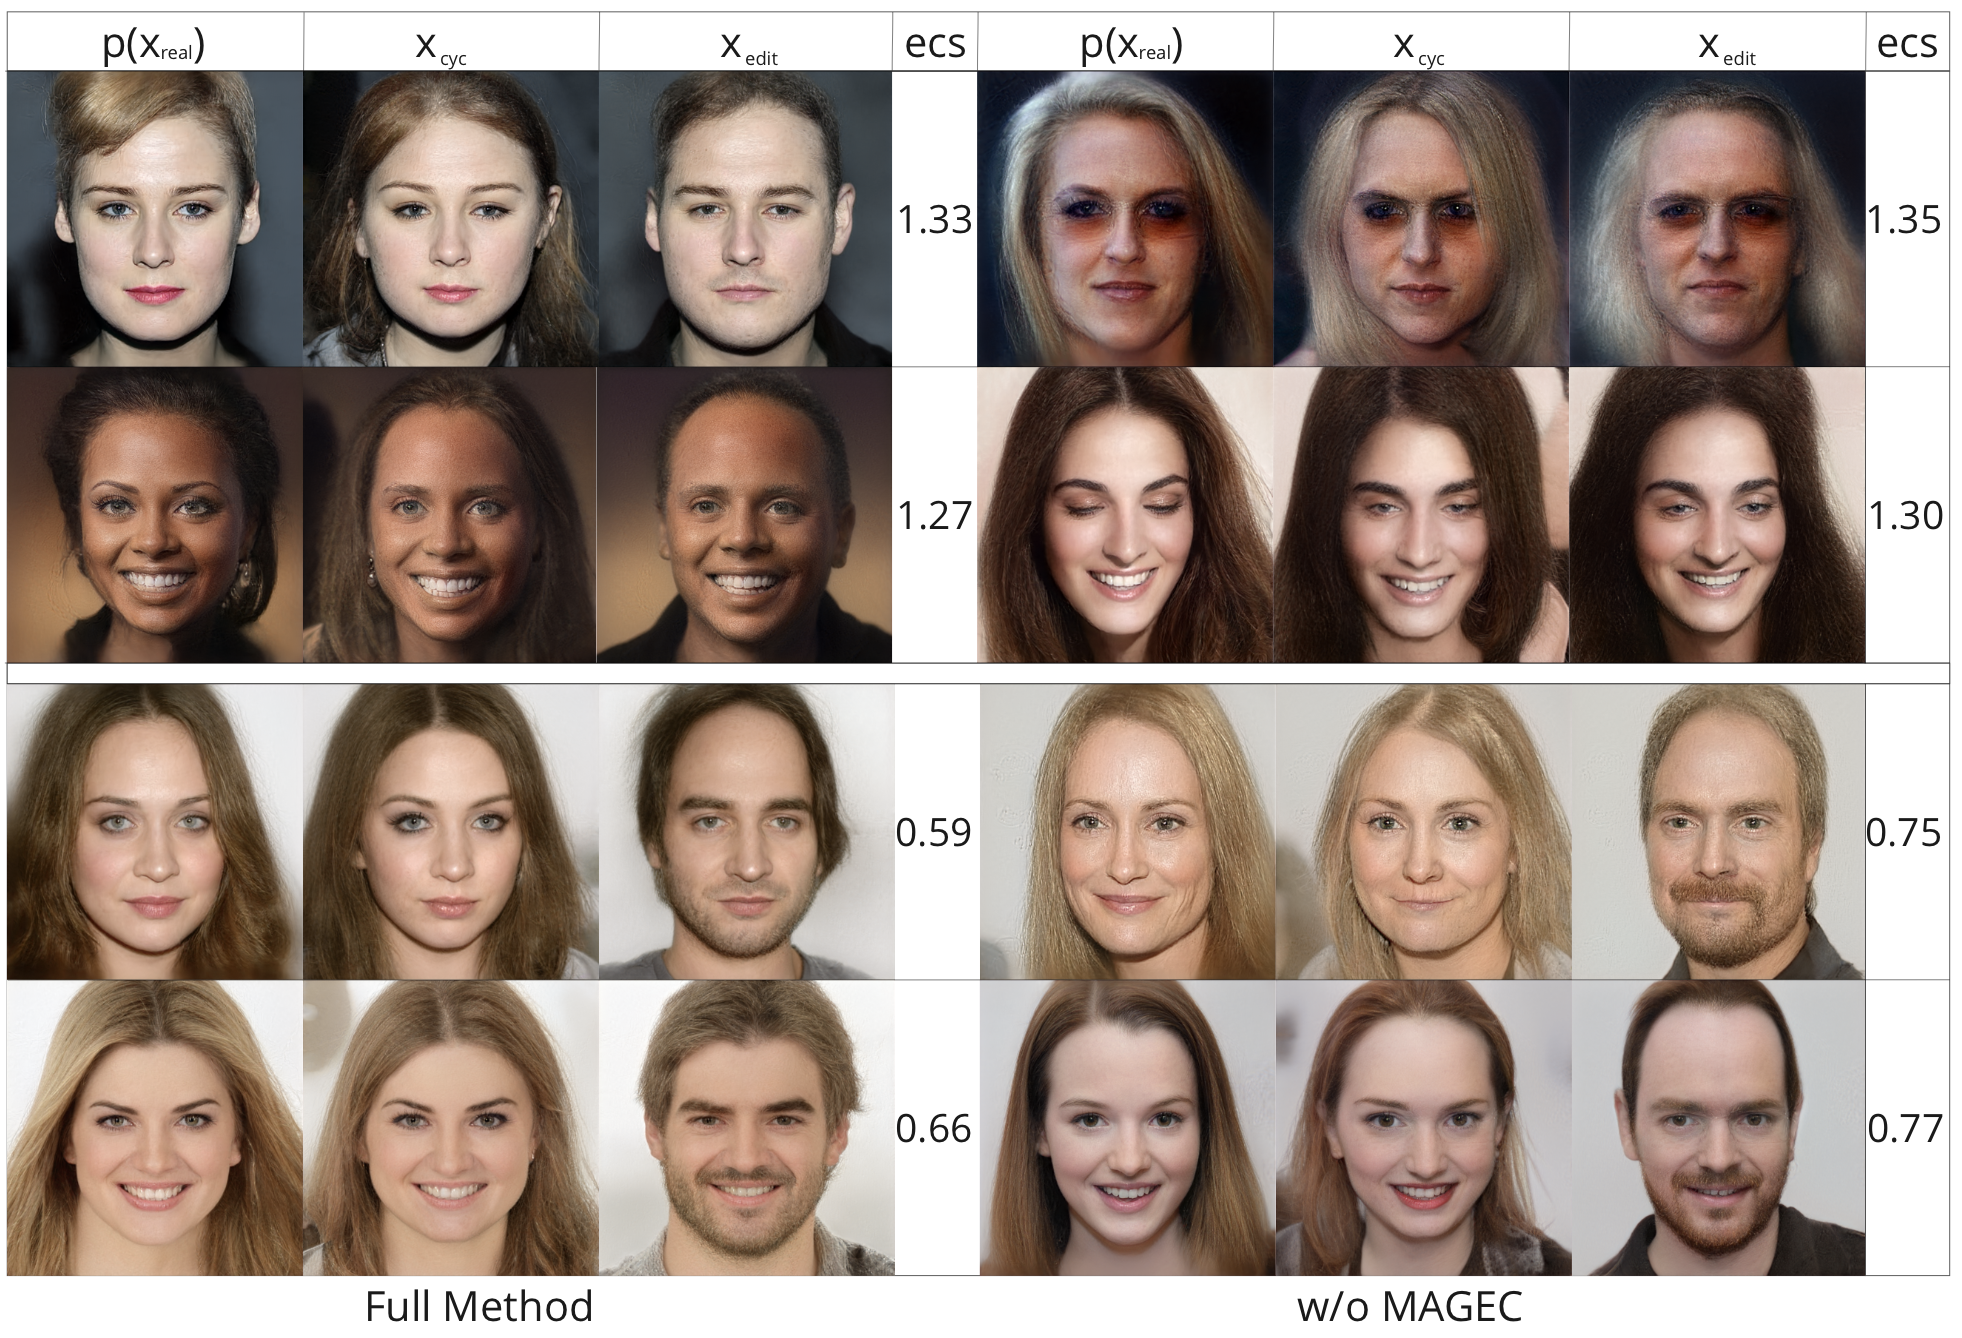
\includegraphics[width=\textwidth]{images/magec/edit_consistencies2.png}
  \caption{Best and worst $ecs$ scores for a given projection method. Here, the editing method is \emph{"to male"} with GANSpace. Notice how the worst scores correspond to poorer editability, for example, the woman in the second row on the right did not transform into a man.}
  \label{fig:ecs_examples}
\end{figure*}





% \begin{figure}[h]
%     \centering   
%    \subfigure[]{\label{fig:User_interface}
\includegraphics[width=63mm, valign=m]{images/magec/user_interface_2.png}}\hspace*{\fill}
%    \subfigure[]{\label{fig:userstudyresults}
   
%    \begin{tabular}{|l|c|}
%    \hline
%    \multicolumn{1}{|c|}{\textbf{\begin{tabular}[c]{@{}c@{}}Displayed Methods \end{tabular}}} & {\color[HTML]{000000} \textbf{\begin{tabular}[c]{@{}c@{}}\% Preferred\\  Ours\end{tabular}}} \\ \hline
%    Ours vs. w/o MAGEC                                                                                      & 72\%                                                                                         \\ \hline
%    Ours vs. Im2StyleGAN++                                                                                  & 78\%                                                                                         \\ \hline
%    \end{tabular}
%    }
%    \caption{User Study: 30 photography experts judged edit operations resulting from 3 projection methods: (1): Our full method, (2): Ablation of MAGEC loss from our Eq.~\ref{final_loss_term}, and (3): Im2StyleGAN++\cite{abdal2020}. Fig. ~\ref{fig:User_interface} shows the interface in which the expert had to choose their preferred edit according to quality and coherence to the edit operation. The user judged for five minutes, and an average of 30 edit pairs were judged per user. Each edit operation consisted in changing one of 10 possible facial attributes to a random new value, using either \cite{harkonen2020ganspace} or \cite{abdal2020styleflow}. For fairness, \cite{shen2020} was not included in the edits, as this method was used to supervise our loss. The results (Fig. ~\ref{fig:userstudyresults}) show the strong preference for our method.}
   
%    \label{fig:complete_user_study}
%    \end{figure}






\newcommand{\userstudytab}{% Just for this example
\begin{tabular}{|l|c|}
    \hline
    \multicolumn{1}{|c|}{\textbf{\begin{tabular}[c]{@{}c@{}}Displayed Methods \end{tabular}}} & {\color[HTML]{000000} \textbf{\begin{tabular}[c]{@{}c@{}}\% Preferred\\  Ours\end{tabular}}} \\ \hline
    Ours vs. w/o \magec                                                                                      & 72\%                                                                                         \\ \hline
    Ours vs. Im2StyleGAN++                                                                                  & 78\%                                                                                         \\ \hline
    
  \end{tabular}
}

\begin{table}
  \centering
  \userstudytab
  \caption{Results of our human evaluation survey. 30 photography experts 
  were questioned (as shown in Fig.~\ref{fig:user_interface}) to rate our method compared to either our ablated method 
  (Eq.~\ref{final_loss_term} without the \magec loss) or to Im2StyleGAN++ \citep{abdal2020}.
   Each edit operation consisted in changing one of 10 possible facial attributes
   to a random new value, using either GANSpace \citep{harkonen2020ganspace} or 
   StyleFlow \citep{abdal2020styleflow}. For fairness, InterfaceGAN \citep{shen2020} was not included 
   in the edits, as this method was used to supervise our loss. The results 
   show the strong preference for our method.}
  \label{tab:userstudyresults}
\end{table}

\begin{figure*}
  \centering
  
\includegraphics[width=0.8\textwidth]{images/magec/user_interface_2.png}
  \caption{Interface provided for human evaluators. 30 photography experts 
  where presented with an original photo and an edit operation and were asked
   to choose their preferred edited image out of two choices. The user 
   judged for five minutes and an average of 30 edit pairs were judged per user.}
  \label{fig:user_interface}
\end{figure*}





\section{Limitations of our Method}\label{section:magec_limitations}




Our method aims at producing an editable latent vector, which often means a 
vector within the domain of the pre-trained GAN. Using real images that are 
clearly out of domain produces low-quality results, both in terms of 
reconstruction and editability. This is because the trade-off between these
 two objectives is too strong, and our method struggles to find a suitable
  compromise. See the top row of Fig.~\ref{fig:problem_images} for an example.
  Our method also fails when faced with rare or challenging semantics. 
The \magec loss is not sufficient to push the $\z$ in the ideal direction, 
and some semantic concepts  become lost. As we see in the bottom row of 
Fig.~\ref{fig:problem_images}, the keffiyeh becomes semantically represented 
as hair.

\begin{figure*}
\centering

    \includegraphics[width=0.75\textwidth]{images/magec/problem_images.png}

\caption{Problematic images for our method. In the first row, an atypical face 
produces a low-quality reconstruction since the image space loss and the latent 
space loss oppose each other: the input image is too out-of-domain. In the
 second row, our method struggles to represent a challenging semantic concept 
 (the keffiyeh). The projection represents the keffiyeh as hair, 
 evidenced by the subsequent edits (\emph{straight hair}, \emph{old age}).}
    \label{fig:problem_images}
\end{figure*}



\section{Conclusion}

We propose a novel GAN-inversion optimization strategy which 
allows supervision on two levels: the image space and the latent
 space. In this way, we are able to integrate editability directly
  in the loss term, resulting in more editable latent vectors when
   applying editing methods. In particular, editing methods not 
   used to supervise the loss perform better than baseline methods,
    suggesting that performing optimization in this way discovers 
    a more ``in-domain'' latent vector. We evaluate qualitatively 
    and quantitatively, and notably introduce a novel 
    \emph{edit consistency score} which specifically evaluates the
     performance of a projection method in terms of editability.
      Our method takes a step forward in performing realistic and 
      high-quality edits on real images.


% In concurrent work, \cite{alaluf2021restyle} proposed an 
% encoder-based method based on \emph{iterative refinement}, in which the latent 
% vector is passed and refined through an encoder multiple times, ressembling 
% the iterative denoising nature of a \ac{DDPM}. They obtained state-of-the-art 
% results for encoder-based methods, and only required 10 forward passes, but their 
% reconstruction still lagged behind optimization-based methods. 
In  concurrent work on optimization-based methods, 
BDInvert \citep{kang2021gan} proposed an inversion method specifically to address the 
poor inversion for out-of-domain translated or rotated images, by extending the 
optimization space to include a feature map in the convolutional \ac{GAN}, which is invariant
to rotation and translation. Finally, later work \citep{feng2022near} achieve 
state-of-the-art optimization-based inversion results, both in terms of editing and reconstruction.
They propose a clever strategy which addresses the limitations posed in section \ref{section:magec_limitations}
by first finding the closest latent $\z$ possible through an encoder-based method 
or optimization-based method, and then optimizing the parameters of the \ac{GAN}
itself to actually change and adapt its manifold to include out-of-domain images 
within its manifold. Because only small tweaking is required to adapt the pre-trained 
\ac{GAN}'s manifold, existing editing methods still work out-of-the-box.

Nevertheless, \ac{GAN} inversion methods are still limited to images from restricted 
domains of a pre-trained \ac{GAN}, largely limiting their use-case to practical settings. 
In the next chapter, we thus try to circumvent inversion completely and examine image 
editing through the lense of optimizing a VQ-GAN \citep{esser2021taming} encoded vector 
before decoding the edited embedding. 


\cleardoublepage
\let\leftmark=\oldleftmark

\acresetall
\chapter{Text-Guided Image Editing}
\label{chapter:flexit}


\chapterwithfigures{\nameref*{chapter:flexit}}
\chapterwithtables{\nameref*{chapter:flexit}}

\ifthenelse{\boolean{skipFlexit}}{\endinput}{}

\section{Introduction}

Thusfar, we have examined one way of performing semantic-image editing: 
generalizing latent manipulation methods of \ac{GAN}s to real images. For this, 
we saw in the previous chapter that the real image must first be inverted into 
the latent space of a \ac{GAN}, a task that is not trivial and will poorly respond to 
 images out of the \ac{GAN}'s distribution. Moreover, we saw that in general, \ac{GAN}s 
 are highly powerful in generating images of a restricted domain, they are much less 
 efficient in generating high-quality and diverse images of a more diverse domain. 
 However, we strive to perform image editing on any possible image. 
 
 In this chapter, 
 we thus investigate the use of a recently proposed autoencoder, VQ-GAN \citep{esser2021taming}, 
 to bypass this issue and encode any image into a latent "code" directly. 
 
Specifically, we propose  a unified framework which modifies an input image based
 on a user-defined text query of the form $(S \rightarrow T)$, like \textit{cat} → \textit{dog}.
  For this \textit{semantic image translation} task, the goal is to make minimal image
   modifications  while transforming the image as requested.
We leverage \ac{CLIP} \citep{radford2021learning},  which combines text and image representations in 
one powerful multimodal embedding space. This space is used to define our target point,
 based on the embeddings from the user input. We perform a per-image optimization 
 procedure, using specific  strategies to ensure image quality and relevance to the 
 transformation query. Our method requires only fixed pre-trained components, and can 
 thus be used off-the-shelf  without  requiring any training. 

We also propose a quantitative evaluation protocol for the task of semantic image 
translation. 
Evaluation is based on three criteria: (i) the transformed image should correctly 
correspond to the text query, (ii) the output image should look natural,  and (iii) 
visual elements irrelevant to the text query should remain unchanged. 
We thoroughly evaluate our model on ImageNet, and  demonstrate quantitatively and 
qualitatively the superiority of our method against baselines, broadening the horizon 
of text-driven image editing.


In this chapter, after quickly reviewing some related work, we discuss our framework for 
text-guided image editing by leveraging \ac{CLIP} 
and VQ-GAN. Next, we will discuss our evaluation protocol and compare our method to existing baselines, 
showing our superior performance. We further discus our implementation, hyperparameter choices and perform an 
ablation study which show the rigour of our method. Finally, we discuss some limitations of our method and 
conclude. Our work has led to the following publication:

\begin{itemize}
    \item \fullcite{couairon2022flexit}
\end{itemize}



\section{Related Work}


\paragraph{Image latent space}
While GANs are highly effective as generative models, inference of the latent variable 
given an image is not trivial, as we have seen in Chapter \ref{chapter:magec}. 
While joint learning of an inference network has been proposed, \citep{donahue17iclr,dumoulin17iclr}, 
the mode-seeking training dynamics of GANs are 
 not suited for good reconstruction performance beyond the training distribution 
 (or even within it, if modes are dropped).
Variational autoencoders~\cite{Kingma2014}, on the other hand, offer an inference 
network by construction, and their likelihood-based training objective ensures accurate 
reconstructions.

Vector-quantized  variational autoencoders (VQ-VAE)~\cite{oord17nips,razavi2019generating},
 which discretize the latent space, have been found to offer good reconstructions. The prior distribution
 is a categorical distribution and kept constant and uniform during sampling.
 The prior is not trained jointly with with VQ-VAE, and thus, unlike classical \ac{VAE}s (see \ref{section:chapter1_variational_auto_encoders}),
 has no generative capacities until it is made autoregressive (which is done in a next step). 
VQ-GAN \citep{esser2021taming,yu2021vector} further improves reconstructions 
by  including an adversarial loss term to train the autoencoder.
In our work,  we adopt the VQ-GAN autoencoder,  and edit  images in its latent space.



\paragraph{CLIP and Text-Guided image editing}

To align images and text, \ac{CLIP}~\citep{radford2021learning} learns encoders that map both 
modalities to a shared latent space in which they can easily be compared and combined.
 Vision encoders are based on ResNets \citep{he2016deep} and \ac{ViT}s
  \citep{dosovitskiy2020image}.

  \ac{CLIP}, trained on 400M web-crawled image/text pairs with a simple contrastive InfoNCE
 loss \citep{oord18arxiv},  can provide a robust differentiable signal for image
  synthesis and editing, used in conjunction with diffusion 
  models \citep{kim2021diffusionclip}, and  generators based on B\'ezier curve 
  strokes \citep{frans2021clipdraw}. \ac{CLIP} was also successfully used in conjunction
   with VQ-GAN to generate novel art images \citep{vqgan_clip} or perform semantic
    style transfer \citep{vqgan_semantic_style_transfer}.
Similarly to us, StyleCLIP \citep{patashnik2021styleclip} transforms images based
 on text queries via alignment in \ac{CLIP}'s latent space. However it relies on the 
 latent space of StyleGAN2 \citep{karra2020stylegan2} to optimize the image, which requires training a separate 
 generative and latent space inference model per application domain, as we have seen in the previous chapter.

% talk about manigan
As previously discussed in \ref{section:image_editing}, image editing can be guided by 
many conditions e.g. another image, a segmentation map, a class label. Allowing the user 
to provide unstructured free-form text queries is more challenging. 
Close to our objective,  ManiGAN \citep{li2020manigan} aims at performing 
text-based edits by training an editing model to refine the details of an image based on its 
textual description. Their model inputs a text prompt $S$ and an input image $I$ and 
modifies $I$ according to $S$. However, their model is trained on aligned (image, text)
pairs and rely on regularization terms to avoid generating the same image as the input image.
Their GAN-based approach relies on progressive growing as well as attention and modulation 
when fusing image and text embeddings, which are learned through jointly trained text and image encoders. 
They train and evaluate on COCO \citep{lin2014mscocodataset} and CUB datasets \citep{welinder2010cub200}.




\section{FlexIT framework for semantic editing}


An overview of our image transformation approach is depicted in Figure~\ref{fig:flexit_method}. 
It relies on three pre-trained components. 
First, we edit the input image in a  latent space, with the requirement that a wide 
range of  images can be encoded and decoded back to an RGB image with minimal
 distortion. We chose the VQ-GAN autoencoder~\citep{esser2021taming} for that purpose.
Second, we embed the text query and input image in a multimodal embedding space, to 
define the optimization target for the modified image. We use the 
\ac{CLIP}~\citep{radford2021learning} multimodal embedding spaces.
Finally, to ensure that the modified image remains similar to the input, we control 
its distance to the input image with the LPIPS perceptual distance~\citep{zhanglpips2018}
 computed with a VGG~\citep{simonyan2014very} backbone.

 \begin{figure*}[h]
    \centering
    \vspace{-1em}
    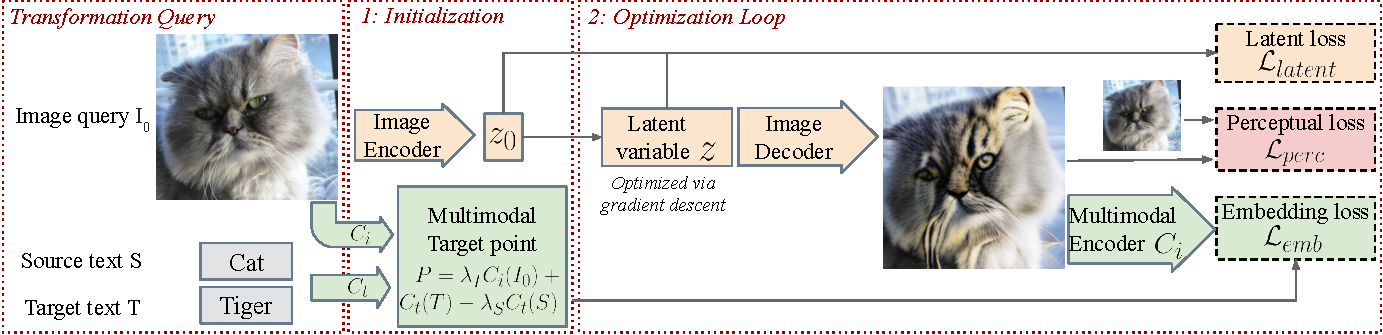
\includegraphics[width=\linewidth]{images/flexit/assets/method.pdf}
    \caption{FlexIT optimization framework: components  involving the multimodal latent space  colored in green; those involving the 
    image latent space in yellow; those involving the LPIPS distance in pink. Given a transformation query $(I_0, S, T)$, we first
     compute a target point $P$ in the multimodal embedding space, and we encode $I_0$ in the image latent space to get $z_0$. Then, 
     for a fixed number of steps, we update the latent variable $z$ (initialized with $z_0$) to get closer to the target point $P$. 
    We  add two regularization terms: the LPIPS perceptual distance between the input image and the output image, and a latent distance
     between $z$ and $z_0$. All networks are frozen, only $z$ is updated.}
    \label{fig:flexit_method}
\end{figure*}


\minipar{Optimization scheme}
The core idea of the FlexIT method is to edit the input image in a latent space, 
guided by a high-level semantic objective defined in the multimodal embedding space.
 Let $E$ be the image encoder, $D$ the image decoder and $(C_t, C_i)$ the multimodal 
 encoders for text and image respectively. Given an input image $I_0$ and a textual 
 transformation $S \rightarrow T$, we first initialize \ours by computing the initial 
 latent image representation as $z_0 = E(I_0)$ and the target multimodal point $P$ as
\begin{equation} 
P = C_t(T) + \lambda_{I} C_i(I_0) - \lambda_S C_t(S). \label{eq:p}
\end{equation}
We choose to use a multimodal embedding space since it allows text and image modalities 
to be combined together in a meaningful way: semantic transformations defined by textual
 embeddings can be applied to images with linear operations \citep{jia2021scaling}. In 
 this context, our target point $P$ can be seen as an image embedding that has been
  semantically modified with textual embeddings, by removing the source class information ($-\lambda_S C_t(S)$) 
  and adding the target class information ($+C_t(T)$). Since we don't know what is the optimal linear 
  combination of image and text embeddings, we consider $\lambda_I$ and $\lambda_S$ as parameters
   which will be validated on our development set.

To find an output image which, when encoded in the multimodal embedding space, gets as close as 
possible to the target point, we optimize the embedding loss: 
\begin{equation}
    \mathcal{L}_{emb}(z) = \Vert C_i(D(z)) - P \Vert_2^2.
\end{equation}


We add two regularization terms to the embedding loss, to encourage that only the content related to the transformation query is changed. 
Without regularization, the optimization scheme can alter any part of the image if this helps in getting closer to the multimodal target point, which we have found to yield unnatural artifacts. 
The distance to the input image $I_0$ is controlled with a LPIPS distance:
\begin{equation}
\mathcal{L}_{perc}(z) = d_{\text{LPIPS}} (D(z), I_0). 
\end{equation}

To enforce staying in parts of the latent space that are well decoded by our image decoder, we use a regularization term with respect to the initial latent code $z_0$. 
We use a $\ell_2$ norm at each spatial position $i$ of the latent code, and sum these norms across  spatial positions to obtain the loss: %a mixed $\ell_{2,1}$ norm:
\begin{equation}
\mathcal{L}_{latent}(z) = \sum_i \Vert z^i - z_0^i \Vert_2.
\end{equation}
This loss encourages sparse $z^i$ changes, \textit{i.e.}\ limiting changes in spatial locations, which is aligned with our 
objective to transform a localized part of the input image.

Finally, note that  $\lambda_I$ in Eq.\ (\ref{eq:p}) also acts as a regularization parameter, by encouraging  the input  and 
output image to be close in the multi-modal embedding space.

The total loss we optimize can be written as:
\begin{equation}
\mathcal{L}_{total}(z) = \mathcal{L}_{emb}(z) + \lambda_p \mathcal{L}_{perc}(z)  + \lambda_z \mathcal{L}_{latent}(z).
\end{equation}
After initialization, 
the latent image variable $z$ is updated via gradient descent with a fixed learning rate $\mu$ for a fixed number of steps $N$, 
while keeping all network weights frozen. Following the implementation of the Fast Gradient Method~\citep{dong2018boosting}, 
we normalize the gradient before the update.




\begin{figure}[h]
    \centering
    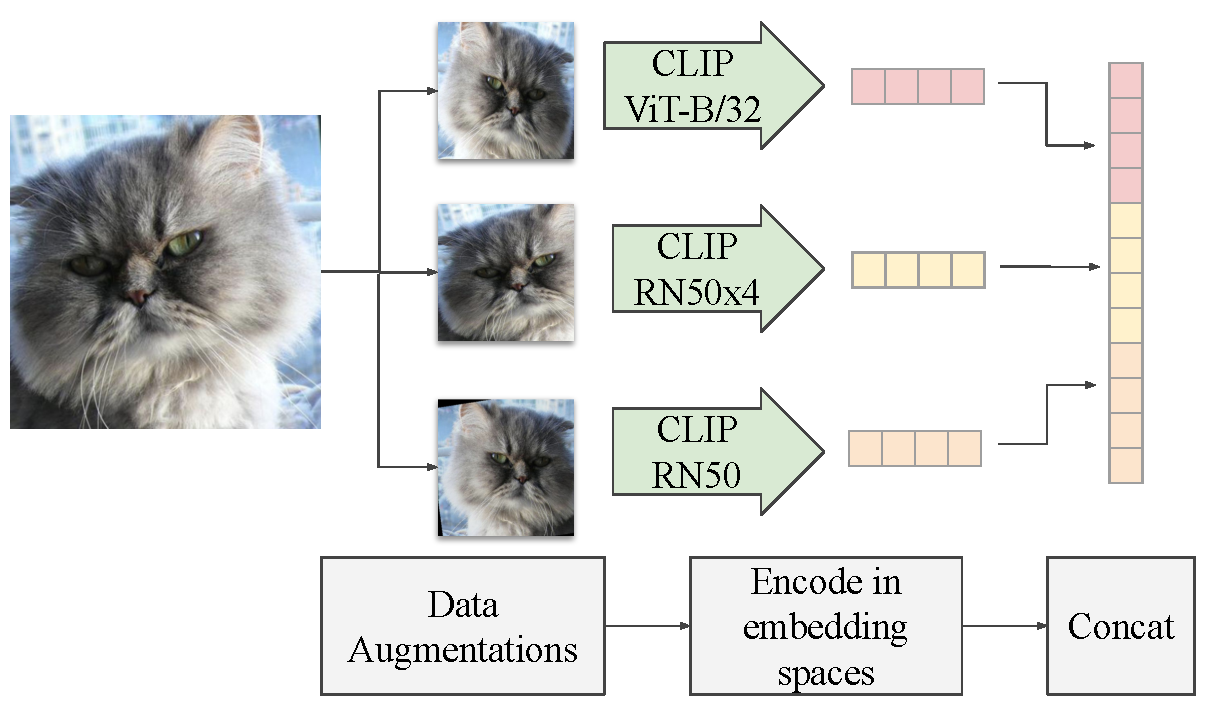
\includegraphics[width=\linewidth]{images/flexit/assets/clips.pdf}
    \caption{
    Architecture of our robust \ac{CLIP}-based image encoder, which combines three different  encoders by concatenation.}
    \label{fig:clips}
\end{figure}


\minipar{Image optimization space}
The distance to the multi-modal target point is a differentiable loss that can be 
optimized via gradient descent. A straightforward approach consists in performing
 gradient descent directly in the pixel-space. However, this type of image 
 representation lacks a  prior on low-level image statistics. 
By optimizing over a  latent variable instead, the  image is obtained as the
 output of a neural-network based decoder. Choosing an autoencoder, like that of 
 VQGAN, lets us (i) make use of the decoder's low-level priors, which guides the 
 optimization problem towards images that exhibit at least low-level consistency;
  and (ii) encode and decode images in its latent space with little distortion. 
  The spatial dimensions in the VQ-GAN latent space allows to edit specific parts
   of the image independently, contrary to \ac{GAN}s which typically rely on more global 
   latent variables. 
Although \ac{GAN}s generate realistic images with stronger priors, it is problematic to
 optimize their latent space for two reasons: first, \ac{GAN}s work  well on narrow 
 distributions (such as human faces), but do not work as well when trained  on a much 
 wider distribution;
second, even with a \ac{GAN} trained on a wide distribution such as that of ImageNet, it
 is hard to faithfully reconstruct  an image using its  latent space.

We report on experiments with optimization over raw pixels and \ac{GAN} latent spaces in  
Section~\ref{ablations}.



\section{Experimental Setup}


\subsection{Implementation details}\label{sub_section:implementation_details}

In \ours, we run the optimization loop for $N=160$ steps, which we found enough to 
transform most images. We use a resolution of 288 for encoding images with VQ-GAN,
 which compresses the images in a latent space with dimensions (256, 18, 18). 

We take advantage of  various pre-trained \ac{CLIP} models, and combine their embeddings
 with concatenation, as shown in Figure~\ref{fig:clips}. 

For the \ac{CLIP}-based multimodal encoders, we have considered all \ac{CLIP} networks freely available, listed in Table~\ref{tab:clip}.
 
\begin{table}[h]
\center
\begin{tabular}{lcc}
\toprule
\textbf{Backbone} & \textbf{Params.} & \textbf{Latent dim.}\\
\midrule
RN50 & 38M & 512\\
RN50x4 & 87M & 640\\
ViT-B/32 & 88M & 512\\
ViT-B/16 & 86M & 512 \\
RN50x16 & 167M & 768\\
\bottomrule
\end{tabular}
\caption{Visual backbones used for the multimodal encoder. Our default configuration only includes the ViT-B/32, the RN50 and the RN50x4.}
\label{tab:clip}
\end{table}

By default, we use three image embedding networks with two different ResNets  and one \ac{ViT} 
architectures, which implement complementary inductive biases.

To encode an image with a single \ac{CLIP} network, we average the embeddings of multiple
 augmentations of the input image. 
 For data augmentations, we use a random horizontal flipping and a random rotation between $-10$ and $10$ degrees, 
 followed by cropping the image (keeping at least $80\%$ of the input image) with aspect ratio between $0.9$ and $1.1$.


For the regularization coefficients, we use 
$\lambda_z=0.05,$ $\lambda_p = 0.15,\ \lambda_S=0.4,\ \lambda_I = 0.2$ as our 
default values. 
These coefficients are set using 
our ImageNet-based development set, and are fixed for all experiments. 


These implementation choices are analysed in Section~\ref{hparam}.



\subsection{Evaluation dataset} 
We did not find a satisfying evaluation framework to study the problem of semantic image
 translation: existing dataset and metrics focus on narrow image domains, or random text
  transformation queries~\citep{li2020manigan,patashnik2021styleclip}. 

To overcome this, we have decided to build upon the ImageNet dataset~\citep{deng2009imagenet}
 for its diversity and its high number of classes: by defining which class labels can be
  changed into one another (like \textit{cat} $\rightarrow$ \textit{tiger}), we can
   build a set of sensible object-centric transformation queries. 

We have selected a subset of the 273 ImageNet labels that we manually split into 47 
clusters according to their semantic similarity as given by the WordNet hierarchy of classes.
For instance, there is a cluster 
containing all kinds of vegetables. 
The resulting clusters are shown in Table~\ref{fig:clusters}. 
 We have not included all ImageNet classes 
because (i) we wanted to reduce the large number of dog breed classes, and (ii) a 
lot of classes were ``standalone classes'' with no natural target for transformation 
among the other classes.

%
We only consider  transformations  $S \rightarrow T$ where $S$ and $T$ are in the same 
cluster, in order to avoid nonsensical transformations between unrelated objects, \eg 
laptop $\rightarrow$ butterfly.

For each target label $T$ we construct eight transformation queries by randomly 
sampling eight other classes $\{S_i\}$ within the same cluster, and sample a random 
image from each $S_i$ from the ImageNet validation set.
This gives  a total of 2,184 transformation queries that we split into a development
 set and a test set of equal size.
We use the development set to tune various hyper-parameters of our approach, and 
report evaluation metrics on the test set.


\renewcommand\cellgape{\Gape[1pt]}
\begin{table}
\tiny
\center
\begin{tabular}{lll}
\toprule
\thead[l]{Group} & \thead[l]{Cluster} & \thead[l]{Classes} \\
\midrule
bird & bird of prey & bald eagle, kite, great grey owl \\
bird & finch & indigo bunting, goldfinch, house finch, junco \\
bird & grouse & black grouse, prairie chicken, ptarmigan, ruffed grouse \\
bird & seabird & king penguin, albatross, pelican, European gallinule, black swan \\
bird & wading bird & goose, oystercatcher, little blue heron, black stork, bustard, flamingo, spoonbill \\
\midrule
container & bag & backpack, plastic bag, purse \\
container & food container & \makecell[l]{water jug, beer bottle, water bottle, wine bottle, coffee mug, vase, \\coffeepot, teapot, measuring cup, cocktail shaker} \\
\midrule
device & electronics & \makecell[l]{cassette player, cellular telephone, computer keyboard, desktop computer, \\dial telephone, hard disc, iPod, laptop} \\
device & measuring & analog clock, digital clock, wall clock, stopwatch, digital watch, odometer, barometer \\
\midrule
dog & hound & English foxhound, Italian greyhound, Afghan hound, basset, beagle, otterhound \\
dog & sporting dog & English springer, cocker spaniel, golden retriever, Irish setter \\
dog & terrier & \makecell[l]{American Staffordshire terrier, wire-haired fox terrier, standard schnauzer, \\Border terrier, Irish terrier, Yorkshire terrier} \\
dog & toy dog & papillon, Chihuahua, Japanese spaniel, Shih-Tzu, toy terrier \\
dog & working dog & \makecell[l]{collie, German shepherd, Rottweiler, miniature pinscher, \\French bulldog, Siberian husky, boxer, Eskimo dog} \\
\midrule
edible & edible fruit & Granny Smith, strawberry, lemon, orange, banana, custard apple, fig, pineapple, pomegranate \\
edible & sandwich & cheeseburger, hotdog, bagel \\
edible & vegetable & \makecell[l]{bell pepper, broccoli, cauliflower, spaghetti squash, zucchini, \\butternut squash, artichoke, cardoon, cucumber} \\
\midrule
fungus & fungus & bolete, coral fungus, earthstar, gyromitra, hen-of-the-woods, stinkhorn \\
\midrule
insect & beetle & ground beetle, ladybug, leaf beetle, long-horned beetle, tiger beetle, weevil \\
insect & butterfly & monarch, admiral, cabbage butterfly, lycaenid, ringlet, sulphur butterfly \\
insect & spider & black widow, garden spider, tarantula, wolf spider, scorpion \\
\midrule
mammal & bear & American black bear, brown bear, ice bear, sloth bear, giant panda, lesser panda \\
mammal & bovid & ox, ibex, bighorn, gazelle, impala, water buffalo, ram, bison \\
mammal & canine & \makecell[l]{Arctic fox, grey fox, red fox, African hunting dog, dingo, \\coyote, red wolf, timber wolf, white wolf, hyena} \\
mammal & equine & sorrel, zebra \\
mammal & feline & Persian cat, tabby, cheetah, jaguar, leopard, lion, snow leopard, tiger \\
mammal & great ape & chimpanzee, gorilla, orangutan \\
mammal & monkey & capuchin, spider monkey, squirrel monkey, baboon, guenon, macaque \\
\midrule
music. instr. & percussion & chime, drum, gong, maraca, marimba, steel drum \\
music. instr. & stringed & cello, violin, acoustic guitar, electric guitar, banjo \\
music. instr. & wind & bassoon, oboe, sax, flute, cornet, French horn, trombone \\
\midrule
object & ball & golf ball, ping-pong ball, rugby ball, soccer ball, tennis ball \\
object & handtool & hammer, plane, plunger, screwdriver, shovel \\
object & headdress & bathing cap, shower cap, bonnet, cowboy hat, sombrero, football helmet \\
\midrule
reptile & amphibian & bullfrog, tree frog, axolotl, spotted salamander, common newt, eft, European fire salamander \\
reptile & snake & \makecell[l]{rock python, boa constrictor, green mamba, Indian cobra, diamondback, sidewinder, \\horned viper, king snake, green snake, thunder snake} \\
reptile & turtle & box turtle, mud turtle, terrapin \\
\midrule
sea life & aqu. mammal & killer whale, grey whale, sea lion, dugong \\
sea life & bony fish & goldfish, tench, eel, anemone fish, lionfish, gar, sturgeon \\
sea-life & crab & American lobster, Dungeness crab, fiddler crab, king crab, rock crab, crayfish, hermit crab, isopod \\
sea life & shark & great white shark, tiger shark, hammerhead \\
\midrule
vehicle & bicycle & motor scooter, tricycle, unicycle, mountain bike, moped \\
vehicle & boat & speedboat, lifeboat, canoe, fireboat, gondola \\
vehicle & car & ambulance, beach wagon, cab, convertible, jeep, limousine, minivan, sports car \\
vehicle & locomotive & electric locomotive, steam locomotive \\
vehicle & sailing vessel & catamaran, trimaran, schooner \\
vehicle & truck & minivan, police van, fire engine, garbage truck, pickup, tow truck, trailer truck, school bus \\
\bottomrule
\end{tabular}

\caption{Groups and clusters of the ImageNet classes used to define the transformation queries.
}
\label{fig:clusters} 
\end{table}


For results, we report quantitative and qualitative results for images from the ImageNet test set. 
We also show  qualitative results from the Stanford Cars dataset~\citep{KrauseStarkDengFei-Fei_3DRR2013}.
Finally, we also show that our method can used on any image in-the-wild, with the image of a 
sow's ear on Figure~\ref{fig:main_demo}.


\subsection{Metrics}
%
We  evaluate the success of the transformation by means of the \textbf{Accuracy} of an 
image  classifier, which is possible since we use ImageNet class labels as the 
transformation targets.
%
We use a DeiT \citep{touvron2021deit} classifier, which has an ImageNet validation 
accuracy of 85.2\%. 
We judge a transformation  successful if, for the transformed image, class $T$ has
 the highest  probability among the  273 selected classes.
The classifier takes images of size 384$\times$384. Smaller images are upsampled before 
being passed to the classifier.

To assess naturalness of  transformed images, we use the \ac{FID}~\citep{heusel2017gans}.
In particular, because we use a small number of samples, we use the (\textbf{\ac{SFID}}).
In addition to the \ac{SFID}, we use a class-conditional
 SFID score  (\textbf{CSFID}) which is an average of the \ac{SFID} scores computed for each 
 target class separately.
  Please refer to \ref{sec:related_fid} for a detailed description these metrics. 
 Because we compute these scores with a low number of examples 
  for many classes, the \ac{CSFID} score has a high bias, low variance profile on our
   dataset \citep{chong2020effectively}, and we  
 have found it to be reliable and stable. We have noticed that the distance on standard deviations was not very discriminative: 
 since we are modifying images and not generating images from scratch, we already have
  a lot of diversity in the generated images. 
  Experimentally, using $\alpha > 0$ of Equation~\ref{eq:sfid} mostly consisted in
   adding a bias term in this metric, therefore we chose to use $\alpha =0 $ in the (C)SFID scores. 

Since the images we transform are extracted from the ImageNet validation set, we use the ImageNet training set as our 
reference distribution to compute the (C)SFID scores. 
The (C)SFID scores are computed at an image resolution of 256.



The \ac{CSFID} metric is a measure of both image quality and transformation accuracy, as it 
measures the feature distribution distance between the transformed images and the 
reference images from the target class in the %ImageNet 
training set. 
Editing should not change parts of the image that are irrelevant to the transformation
 defined in the text,  \eg the background.  
We use the \textbf{LPIPS} perceptual distance~\citep{zhanglpips2018}  to measure deviation 
from the input image (see \ref{sec:related_lpips}). 
As recommended by the authors, we use the AlexNet~\cite{krizhevsky12nips} backbone to 
compute \ac{LPIPS} distance, when we use it as
an evaluation metric. During training, so as to reduce bias in the \ac{LPIPS} evaluation, we used the 
\ac{LPIPS} distance based on VGG features.

The \ac{LPIPS}  distance is computed at an image resolution of 256, for both evaluation and 
optimization.
All \ac{LPIPS}  scores which we will present have been multiplied by 100 for readibility.

The \ac{LPIPS}  distance cannot distinguish edits which are relevant to the text 
query from those which are not; and we don't know the minimal \ac{LPIPS} distance between 
an image and its closest successful transformation. Still, we argue that it should be 
as low as possible.


\subsection{Baselines}
We consider two extreme configurations as baselines,  which only optimize one of these 
two criteria: (i) The  \textsc{Copy} baseline, which simply copies the input image
 without any modification,
and  (ii) the \textsc{Retrieve} baseline that outputs a random validation image 
labelled with the target class $T$.
We add the \textsc{Encode} baseline that simply passes the input image through the 
VQ-GAN autoencoder. 
We also evaluate  StyleCLIP~\citep{patashnik2021styleclip}, the most relevant 
text-driven image transformation algorithm from the literature. We consider the 
version most similar to our method that embeds images with an ImageNet-trained 
StyleGAN2 (see source in next section). We train our own e4e encoder~\citep{tov2021designing} 
to embed images into this latent space.
StyleCLIP iteratively updates the StyleGAN2 latent representation to maximize the similarity
  with a given text in the \ac{CLIP} latent space. Finally, we evaluate
  ManiGAN~\citep{li2020manigan}, which we have trained on ImageNet with the  implementation from the authors.

\subsection{Assets}

We provide a list of the assets used in our work (datasets, code, and models) in
the Appendix in~\ref{sec:FlexIt assets}.

\section{Qualitative Results}


Qualitative results of FlexIT transformations on ImageNet images are presented in 
Figures~\ref{fig:main_demo} and ~\ref{fig:visuresu}.
Figure~\ref{fig:visuresu} shows successful transformations as well as several
 failure cases. 
To demonstrate the generality of our approach, we also  show examples of color 
transformations for images from the Stanford Cars 
dataset~\citep{KrauseStarkDengFei-Fei_3DRR2013} in Figure~\ref{fig:cars30k}.


\begin{figure}[H]
    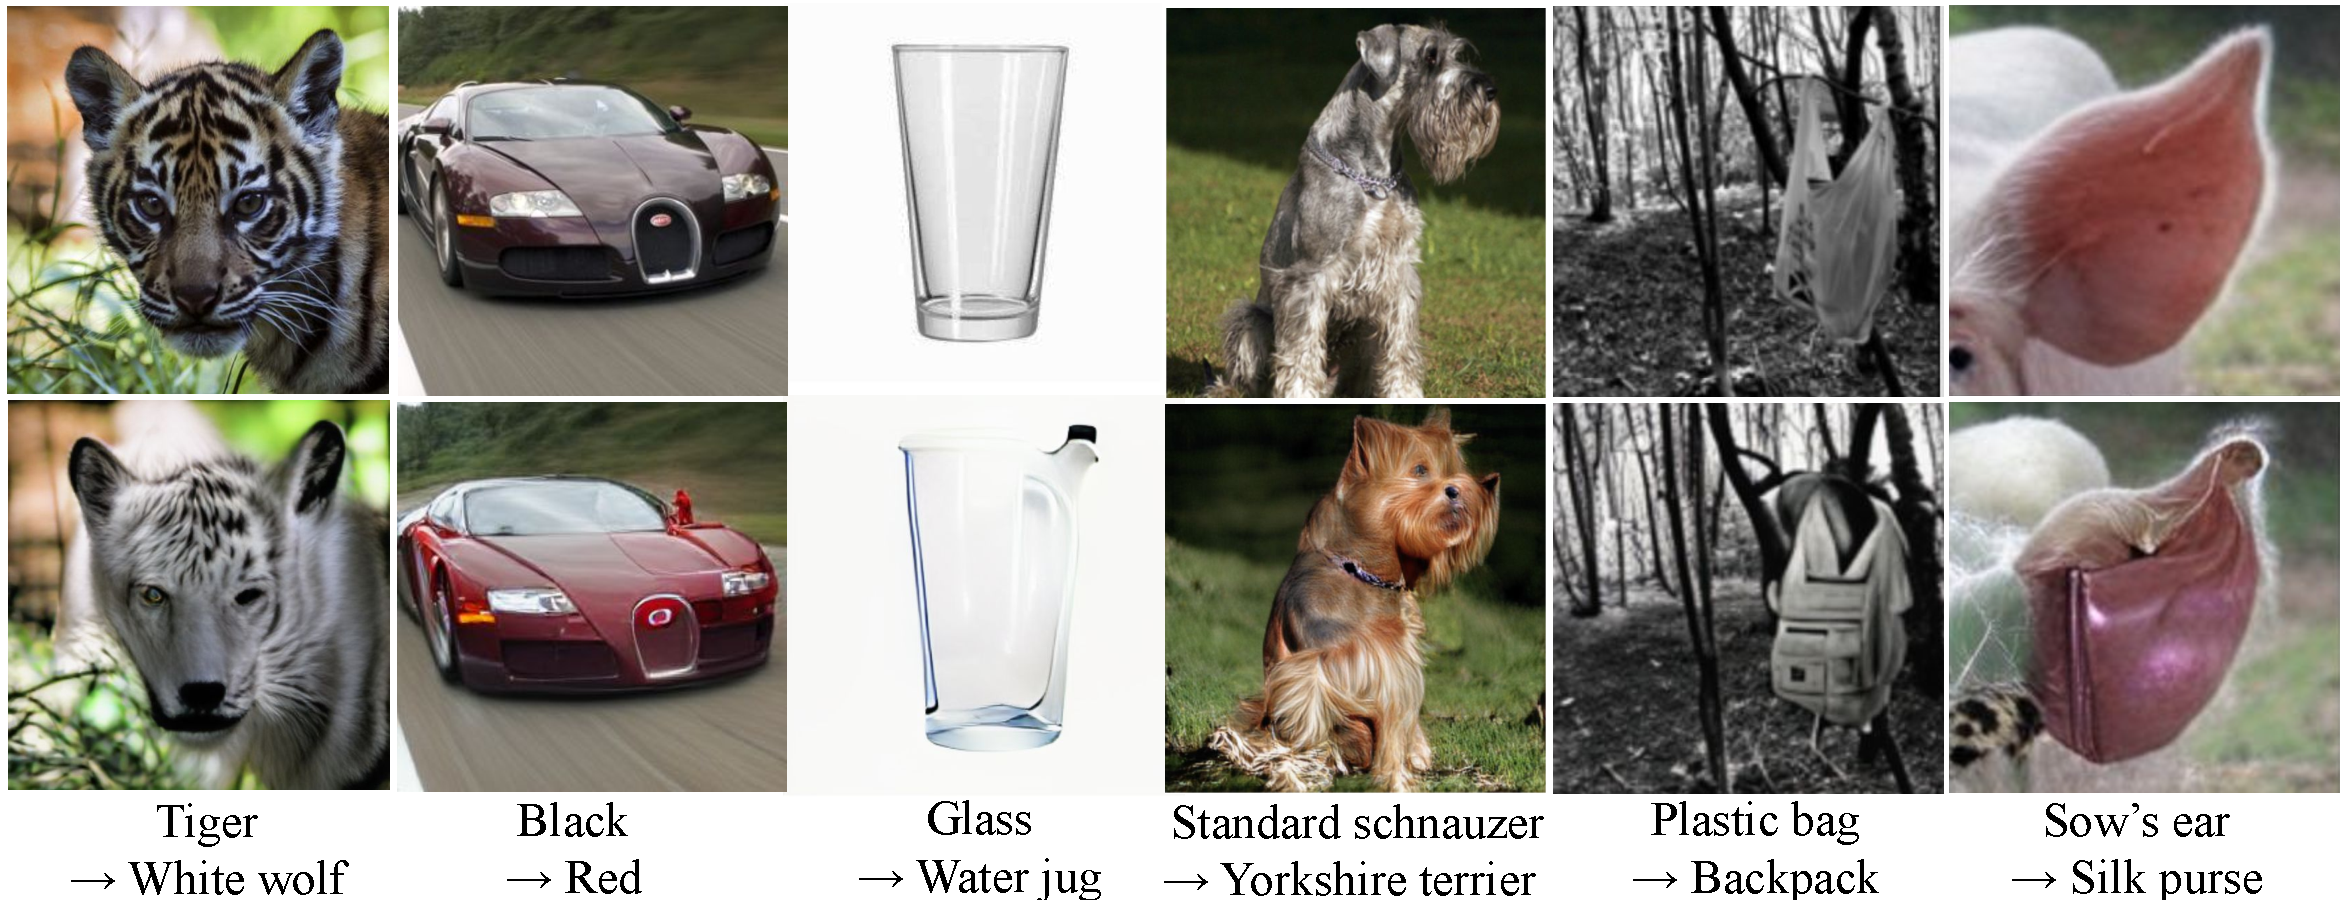
\includegraphics[width=\textwidth]{images/flexit/assets/demo1.pdf}
    \captionof{figure}{\ours transformation examples. From top to bottom: input image, transformed image, and text query.
    }
    \label{fig:main_demo}
\end{figure}

\begin{figure}[H]
    \centering
    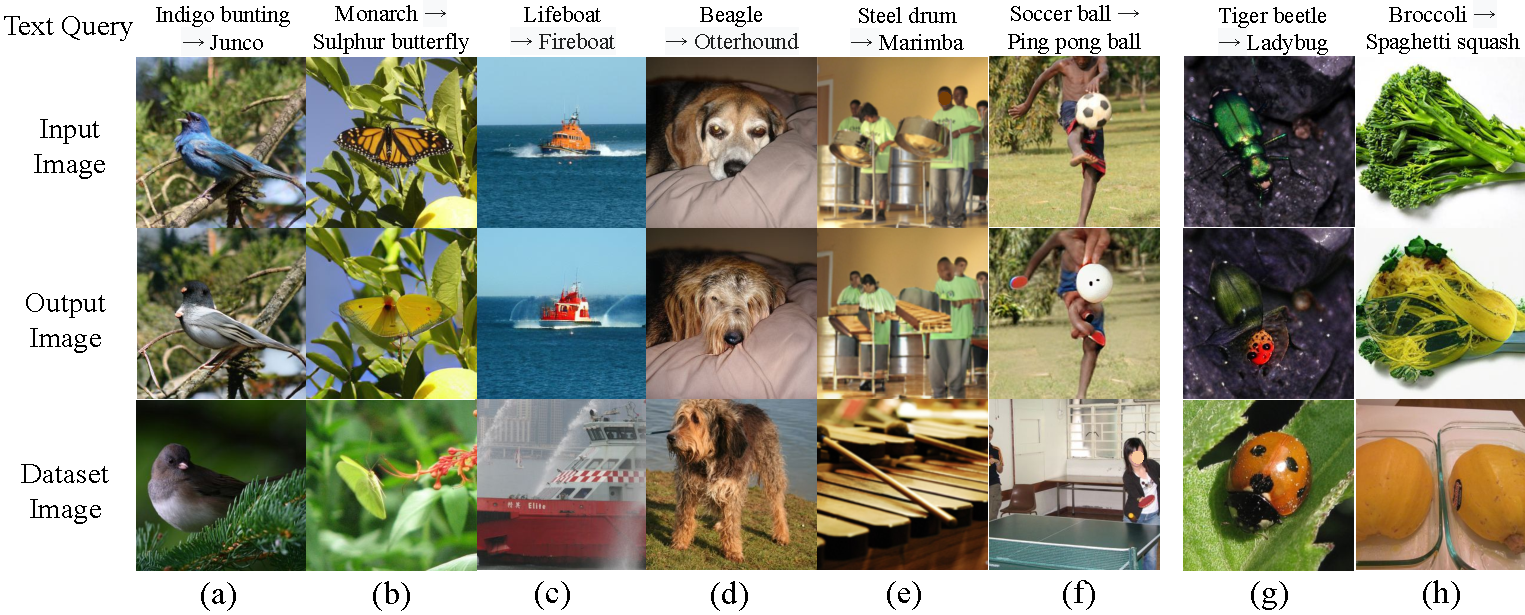
\includegraphics[width=\linewidth]{images/flexit/assets/main_exs.pdf}
    \caption{Transformation examples with \ours on ImageNet images. 
    From top to bottom: input and output image, as well as dataset image from the target
     class.
    Columns (a)-(e) show examples of successful transformations. Column (f) shows an
     interesting behavior where a table tennis racket has been added to add more context. The  last two columns 
      show the most frequent modes of failure: parts of the input image are not changed entirely.
    }
\label{fig:visuresu}
\end{figure}


\begin{figure}[H]
    \centering
    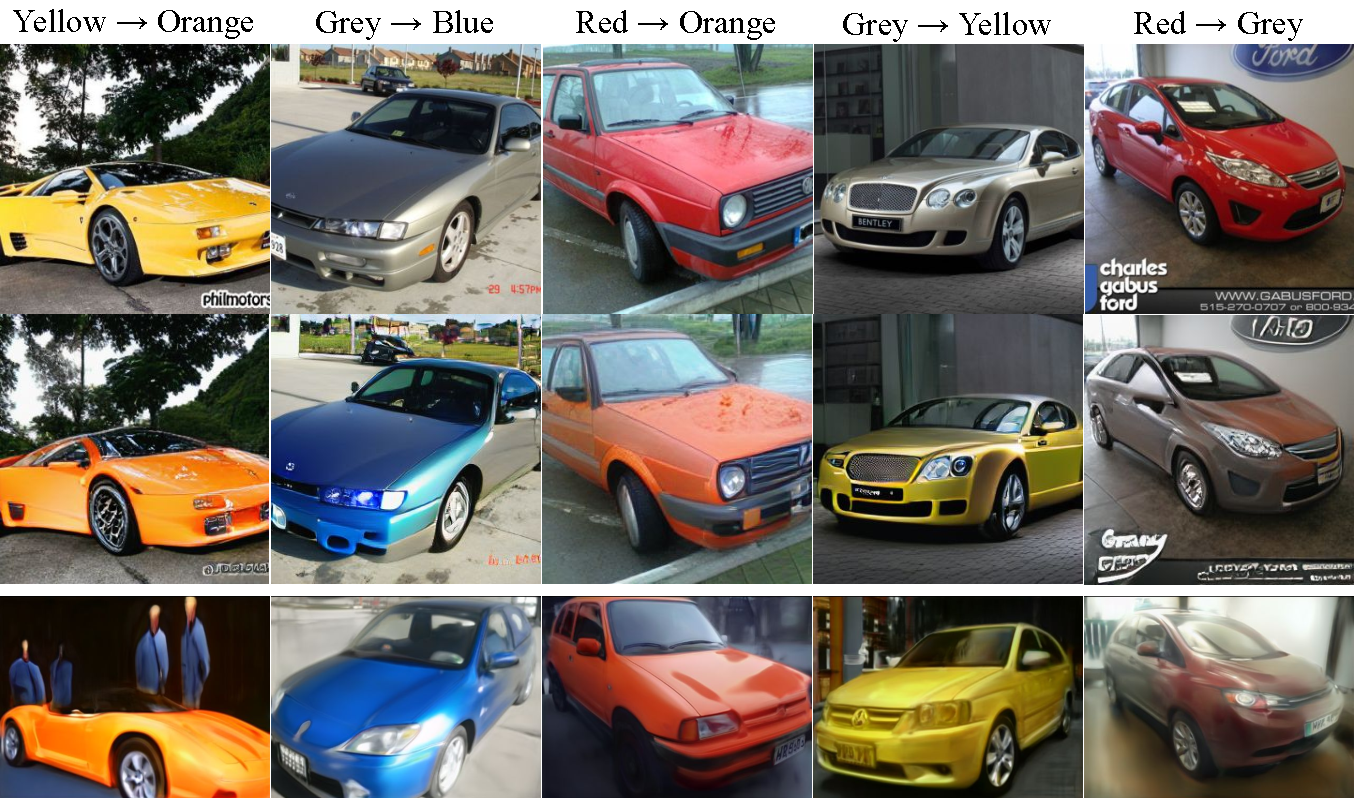
\includegraphics[width=\linewidth]{images/flexit/assets/cars2.pdf}
    \caption{Example  transformations on the \textit{Cars} dataset:  input images (first row),  \ours results  (second row), StyleCLIP results based on a  StyleGAN2 backbone pre-trained on LSUN Cars.
    dataset (last row). Although GAN-based images have better details like the wheels, they are farther away from the input images.}
\label{fig:cars30k}
\end{figure}



\section{Quantitative Results}

Semantic image translation is inherently a trade-off between having the most relevant 
and natural output image (as measured by Accuracy, \ac{CSFID} and \ac{SFID}), while staying as 
close as possible to the input image (as measured by \ac{LPIPS}). 

Results are reported in Table~\ref{tab1}. 
As expected, the copy baseline is ideal on \ac{LPIPS} and \ac{SFID}, but fails to adapt to the 
transformation target $T$, and thus fails on Accuracy and \ac{CSFID}.
For the same reason, the auto-encoding baseline also fails on Accuracy and \ac{CSFID}, but 
demonstrates the non-trivial impact of using the VQ-GAN latent space on \ac{LPIPS} and \ac{SFID}. 
The \textsc{Retrieve} baseline provides ideal metrics for Accuracy, \ac{CSFID} and \ac{SFID}, as 
it returns natural images of the target class. 
It fails  on \ac{LPIPS}, however, since the output image is unrelated to the input. 


\begin{table}[H]
\centering
\small
\resizebox{\columnwidth}{!}{
\begin{tabular}{lrrrr}
\toprule
& \thead{LPIPS ↓} & \thead{Acc.\%↑} & \thead{CSFID ↓} & \thead{SFID ↓}  \\
\midrule
\textsc{Copy} & 0.0 & 0.45 & 106.0 & 0.2 \\
\textsc{Encode} & 17.5 & 1.6 & 107.5 & 3.0 \\
\textsc{Retrieve} & 72.4 & 90.6  & 27.2 & 0.2 \\
%ManiGAN~\cite{li20cvpr}    & ? & ? & ? & ? \\
ManiGAN~\citep{li2020manigan} & 21.7 & 2.0 & 123.8 & 17.0 \\ 

StyleCLIP~\citep{patashnik2021styleclip} & 33.4 & 8.0 & 146.6 & 35.8 \\ 
%StyleCLIP+1,000~\cite{patashnik2021styleclip}   
\ours (Ours) & 24.7 & 51.3 & 57.9 & 6.8 \\
\bottomrule
\end{tabular}}
\caption{Evaluation  of \ours and baselines on ImageNet images. %, comparing to baselines and StyleCLIP. 
}
\label{tab1}
\end{table}
%lpips=33.435783. acc=8.058608	csfid=146.609222	sfid=35.824425	




Our \ours approach  combines a  low \ac{LPIPS} (24.7 \vs 17.5 for \textsc{Encode}) with an 
accuracy of 51.3\% and a \ac{CSFID} of 57.9, which is closer to the \ac{CSFID} of
\textsc{Retrieve} (27.2) than that of \textsc{Encode} (107.5).
The StyleCLIP scores are poor, with high \ac{SFID} and \ac{CSFID} scores which was expected as 
StyleCLIP has been designed to work well where GANs shine.
The StyleGAN2 model we use, trained on ImageNet, is agnostic to class information and 
cannot synthesize realistic images for all ImageNet classes.
ManiGAN works well when trained on narrow domains with color change transformation 
requests, but we find that it does not produce convincing edits when trained on 
ImageNet.


We argue that our evaluation protocol is well-suited for evaluating text-driven image editing because it 
(1): offers a list of sensible transformation queries and (2) offers a method for evaluating the quality and accuracy 
of the generated result. However, to further compare to ManiGAN~\citep{li2020manigan}, we propose to compare our method 
while following their 
evaluation protocol used in their paper. This consists in using the COCO dataset and (1) choosing 
\textit{random} COCO captions/image pairs and thus leading to noisy transformations and (2) calculating the image-text similarity
 score which was used as a loss term during their training, leading to bias in the final scores. 
 We show the evaluation
 in Tab.~\ref{results_manigan}.
 Here, SIM  is the similarity between the output image and text prompt using their trained-encoders. DIFF corresponds to the $L_1$ pixel 
 difference between the input and output image. Finally, MP is their manipulative precision 
 metric which aims at having a high similarity between the output image and text prompt while preserving a small difference between the input and output images.
 Even with this evaluation, FlexIT improves upon the scores of ManiGAN by a large margin.


\begin{table}[H]
    \centering
    \small
    \resizebox{\columnwidth}{!}{
    \begin{tabular}{lrrrr}
    \toprule
    & \thead{IS ↑} & \thead{SIM ↑} & \thead{DIFF ↓} & \thead{MP ↑}  \\
    \midrule
    %ManiGAN~\cite{li20cvpr}    & ? & ? & ? & ? \\
    ManiGAN~\citep{li2020manigan} & 14.96 & 0.087 & 0.216 & 0.068\\ 
    
    %StyleCLIP+1,000~\cite{patashnik2021styleclip}   
    \ours (Ours) & \textbf{18.19} & \textbf{0.177} & \textbf{0.146} & \textbf{0.151} \\
    \bottomrule
    \end{tabular}}
    \caption{Evaluation  of \ours and ManiGAN on ManiGAN evaluation protocol. They performed random edits on COCO (even if the edits are meaningless)
    and based their metrics off of their Image/Text encoders which were used for training. Despite this, we outperform ManiGAN on their evaluation protocol. %, comparing to baselines and StyleCLIP. 
    }
    \label{results_manigan}
    \end{table}
    %lpips=33.435783. acc=8.058608	csfid=146.609222	sfid=35.824425	
    



\begin{figure}[H]
    \hspace{-1.5cm}
    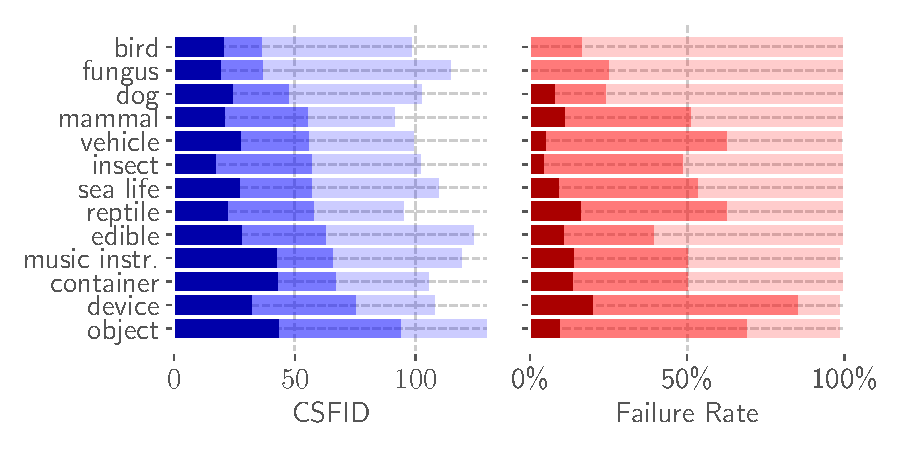
\includegraphics[width=1.2\linewidth]{images/flexit/assets/classwise.pdf}
    \caption{Groupwise CSFID  and Failure Rate (1-Accuracy),  lower is better for both metrics. 
    Dark colors: best possible values obtained with  \textsc{Retrieve} baseline; medium colors: scores obtained with \ours; light colors: values obtained with  \textsc{Copy} baseline. 
    }
\label{fig:classwise}
\end{figure}

To provide insight into which transformations work well, and which less so, we group 
our 47 ImageNet clusters into 13 bigger groups and report 
the average \ac{CSFID} and failure rate ($1 -$accuracy) scores for each group in Figure~\ref{fig:classwise}.
Generally, transformations among  natural objects are more successful than
 transformations among man-made objects. We believe that this is mostly because the 
 latter appear in a wider variety of shapes and contexts which leads to more difficult 
 transformations.




\section{Ablation studies\label{ablations}}


\begin{figure}[h]
    \centering
    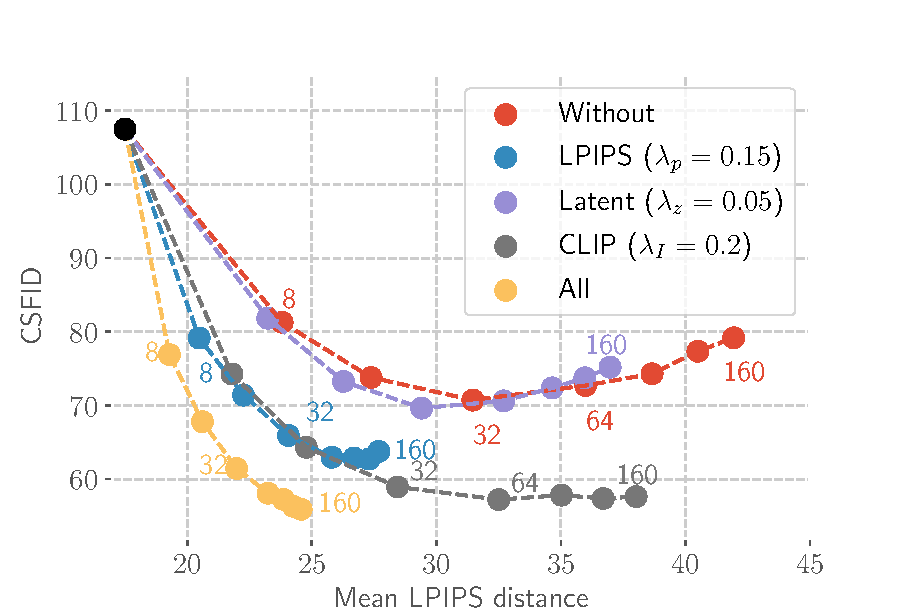
\includegraphics[width=\linewidth]{images/flexit/assets/reg_evol.pdf}
    \caption{\ac{CSFID} obtained without regularization, with individual \ac{LPIPS}, Latent and \ac{CLIP} regularizers, and using all. 
    Each dot corresponds to different amount of optimization steps on the dev.\ set. 
    }
\label{fig:regul}
\end{figure}



\subsection{Regularizers}
In Figure~\ref{fig:regul}, we show the evolution of \ac{CSFID} along the optimization steps, 
where we consider our method without regularization, with each regularization scheme 
separately, and with all regularizers (default configuration).
Compared to not using regularization, the \ac{LPIPS} regularization substantially improves
 the \ac{CSFID} score along the optimization path, while also reducing \ac{LPIPS} as expected. 
The \ac{CLIP} regularizer has a similar effect, but is able to reduce  \ac{CSFID} further while
 the \ac{LPIPS} distance is only slightly reduced compared to our method without any 
 regularization.
%We believe that 
These two regularizers are complementary: while the \ac{LPIPS} loss mitigates image 
deviation for local features, the \ac{CLIP} loss provides semantic guidance which helps to 
reconstruct recognizable objects. %details like faces.
Using all regularizers allows us to obtain the lowest \ac{CSFID} scores at low \ac{LPIPS}. 
Corresponding qualitative examples are shown in Figure~\ref{fig:demo_reg}. We show that 160 
optimization steps is a good value for \ac{LPIPS} and \ac{CSFID} scores. Figure~\ref{fig:steps} shows a 
qualitative example of the effect of optimization steps on the result. While many edits only require 32 steps to be 
completed, some edits benefit from longer optimization schemes.


\begin{figure}[h]
    \centering
    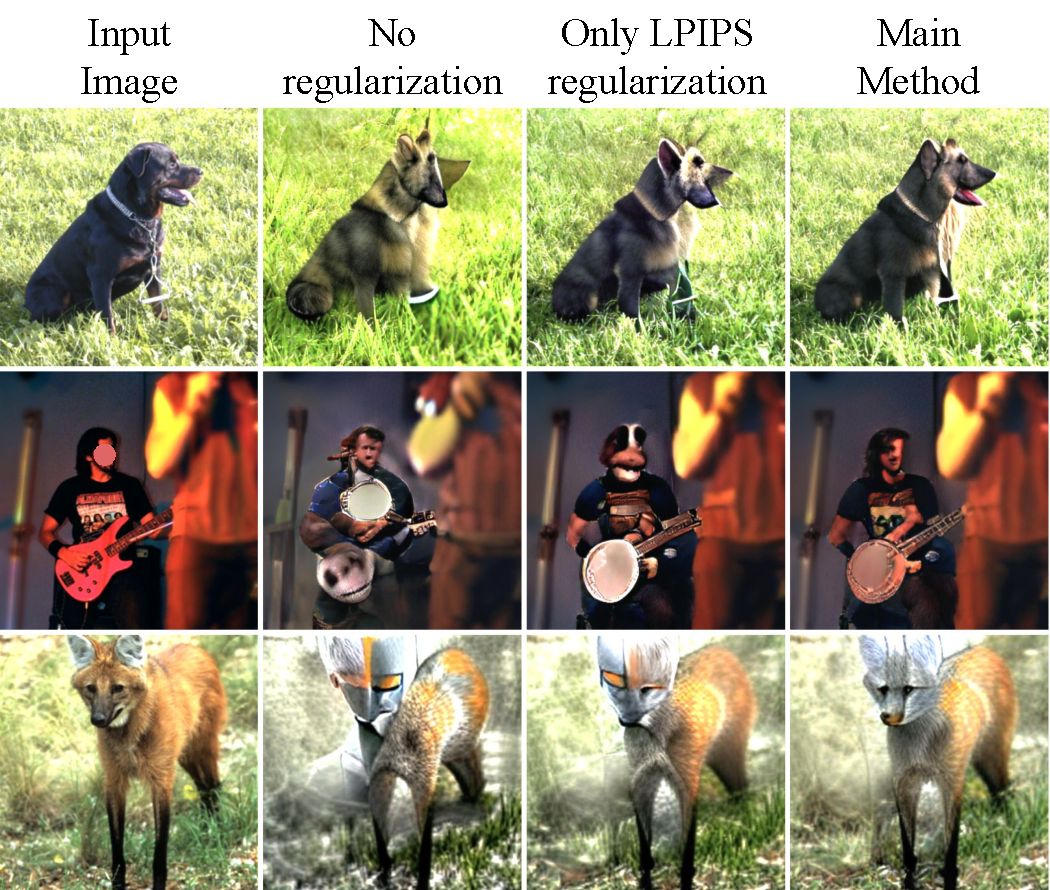
\includegraphics[width=\linewidth]{images/flexit/assets/demo_reg2.pdf}
    \caption{Example transformations with different regularizers. Textual queries from top to bottom: Rottweiler → German shepherd, Electric guitar → Banjo, Red wolf → Grey fox.
    }
\label{fig:demo_reg}
\end{figure}


\begin{figure}[H]
    \hspace{-2cm}
    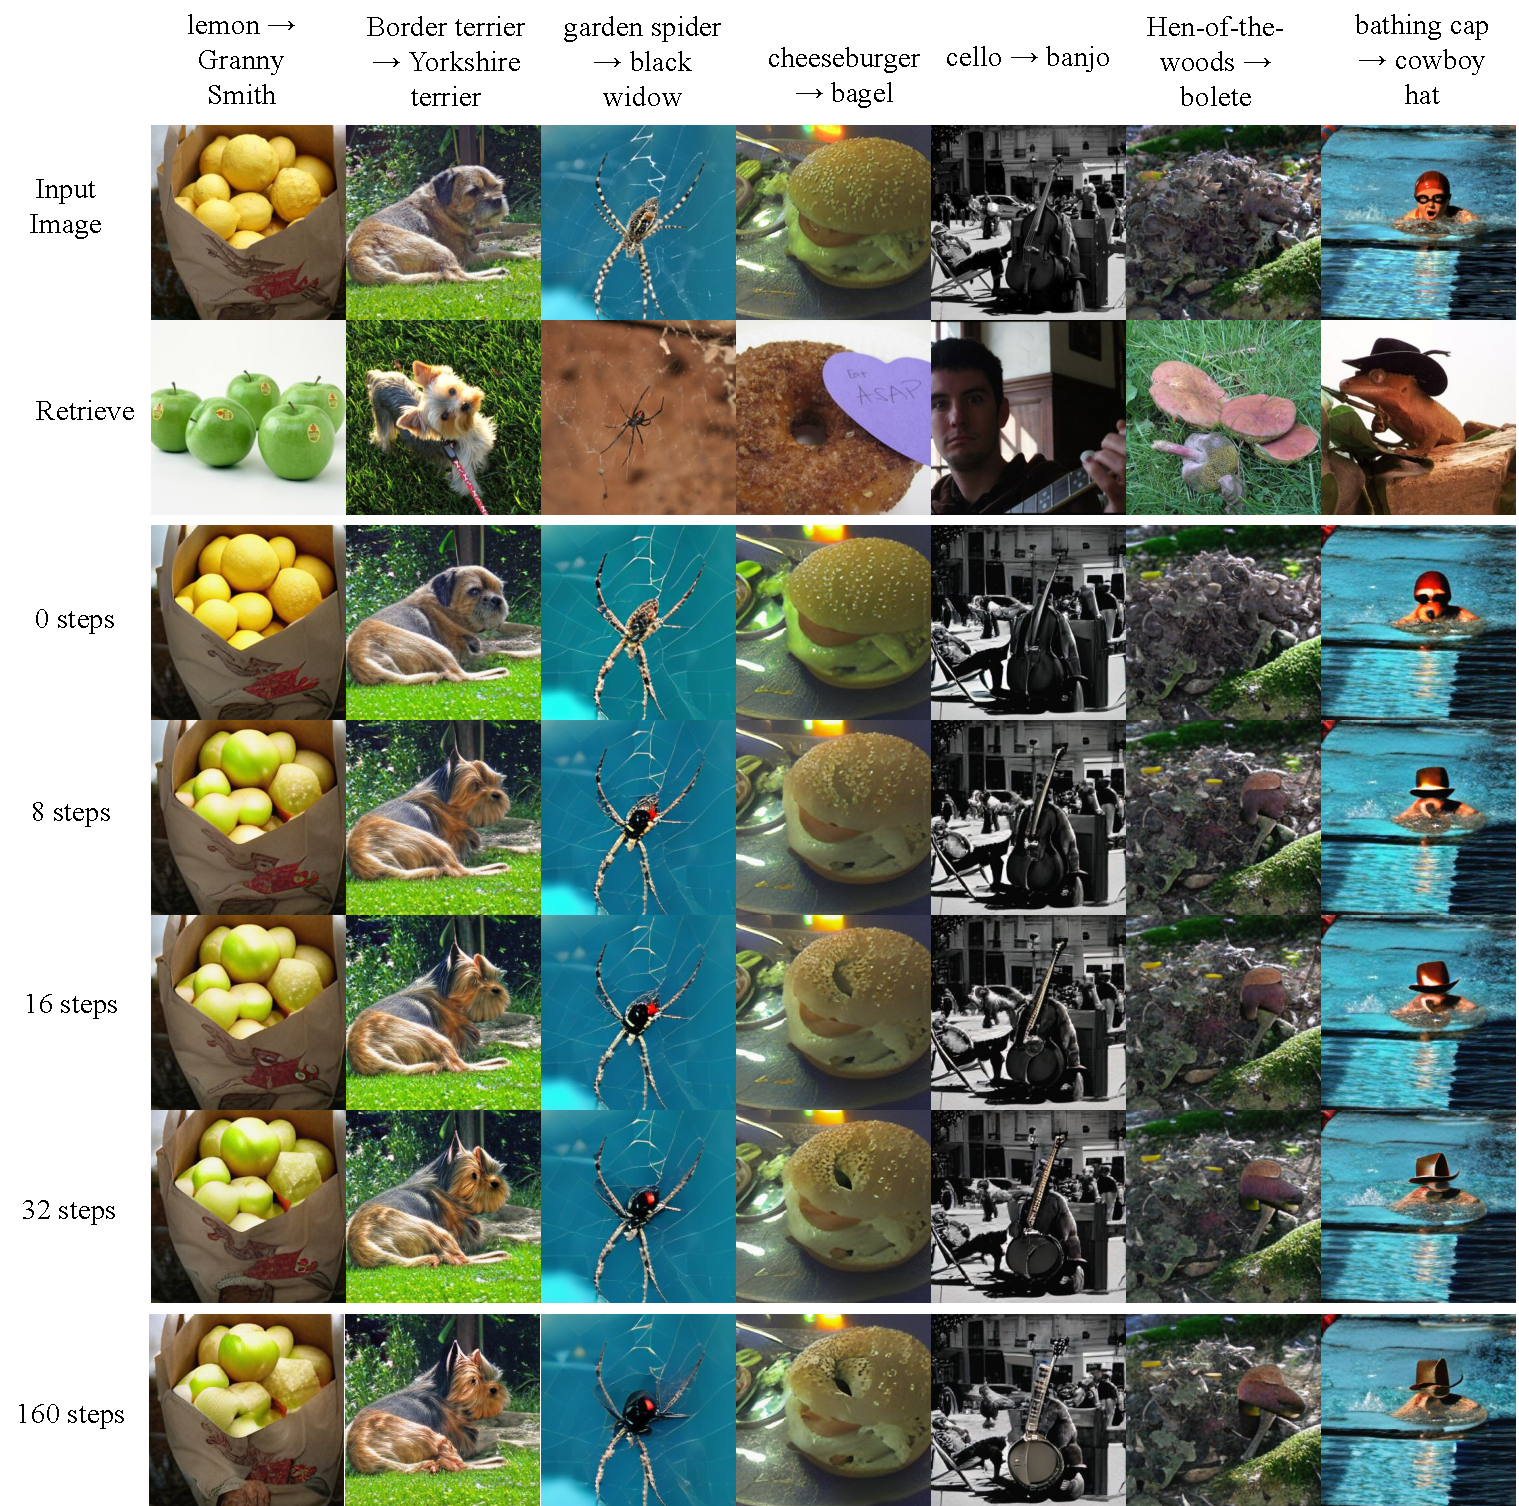
\includegraphics[width=1.2\linewidth]{images/flexit/assets/steps.pdf}
    \caption{Intermediate transformation results obtained with FlexIT. Note that most edits only require 32 steps to be completed; some edits benefit from longer optimization schemes, such as the  spider and the banjo.
    }
    \label{fig:steps}
\end{figure}





In Table~\ref{table:ablations}, we detail the ablation experiments for all FlexIT parameters.

\begin{table}[H]
\center
\begin{tabular}{lrrrr}
\toprule
 & \textbf{Acc.↑} & \textbf{LPIPS↓} & \textbf{CSFID↓} & \textbf{SFID↓} \\
\midrule
                   $\lambda_I=0$ & \textbf{64.8} &   27.6 &   65.4 & 12.3 \\
                   $\lambda_I=0.1$ & 60.6 &   25.9 &   57.8 &  8.3 \\
                     
                    \rowcolor{LightGrey} $\lambda_I=0.2$   & 52.6 &   24.6 &   \textbf{55.9} &  6.4 \\
                   $\lambda_I=0.3$ & 45.8 &   23.5 &   56.3 &  5.5 \\
                   $\lambda_I=0.4$ & 38.6 &   \textbf{22.6} &   58.6 &  \textbf{5.0} \\
                   \midrule
                   $\lambda_S=0.0$ & 34.3 &   \textbf{23.8} &   60.2 &  \textbf{4.8} \\
                  $\lambda_S=0.2$ & 45.9 &   24.0 &   57.3 &  5.5 \\
                  \rowcolor{LightGrey} $\lambda_S=0.4$   & 52.6 &   24.6 &   \textbf{55.9} &  6.4 \\
                  
                   $\lambda_S=0.5$ & 56.2 &   25.0 &   56.5 &  7.1 \\
                   $\lambda_S=0.8$ & \textbf{60.0} &   26.5 &   65.5 & 11.7 \\
                   \midrule
                   $\lambda_z=0.0$ & \textbf{59.4} &   26.5 &   56.1 &  7.1 \\
                   \rowcolor{LightGrey} $\lambda_z=0.05$& 52.6 &   24.6 &  \textbf{55.9} &  6.4 \\
                   $\lambda_z=0.1$ & 51.0 &   \textbf{23.3} &   56.7 &  \textbf{6.3} \\
                   \midrule
                   $\lambda_p=0.05$ & \textbf{66.2} &  28.8 &  \textbf{56.0} &  7.9 \\
                   $\lambda_p=0.1$ & 59.1 &   26.4 &   \textbf{56.0} &  7.2 \\
                   \rowcolor{LightGrey} $\lambda_p=0.15$   & 52.6 &   24.6 &  \textbf{55.9} &  6.4 \\
                   $\lambda_p=0.2$ & 47.9 &   \textbf{23.3} &   57.5 & \textbf{6.3} \\
                   \midrule
                    $\ell_1$ & \textbf{54.2} &   \textbf{24.6} &   56.3 &  6.5 \\
                    $\ell_2$ & 52.4 &   \textbf{24.5} &  \textbf{55.9} &  6.8 \\
                    \rowcolor{LightGrey} $\ell_{2,1}$ & 52.6 &   \textbf{24.6} &  \textbf{55.9} &  \textbf{6.4} \\
                    \midrule
                    $lr=0.025$ & 47.6 &   \textbf{22.5} &   58.3 &  \textbf{6.0} \\
                    \rowcolor{LightGrey} $lr=0.5$     & 52.6 &   24.6 &    55.9 &  6.4 \\
                    $lr=0.1$ & \textbf{60.4} &   27.6 &   \textbf{54.8} &  7.2 \\
                    \midrule
                  resolution 256 & 53.8 &   24.8 &   56.8 &  7.2 \\
                  \rowcolor{LightGrey} resolution 288 & \textbf{52.6} &   24.6 &   \textbf{55.9} &  \textbf{6.4} \\
                  resolution 320 & 54.3 &   \textbf{24.0} &   57.4 &  7.3 \\
                  \bottomrule
\end{tabular}
\caption{\label{table:ablations} FlexIT ablation results. $lr$ is the learning rate. Lines corresponding to our default configuration are marked in light grey. The norms $\ell_1$,  $\ell_2$, and $\ell_{2,1}$  refer to the distance used for regularization in the VQ-GAN latent space. Best values for each metric are shown in bold inside each group of parameter values.
}
\end{table}


\subsection{CLIP embedding module and Data Augmentations} 

\begin{figure}[H]
    \centering
    \vspace{-1em}
    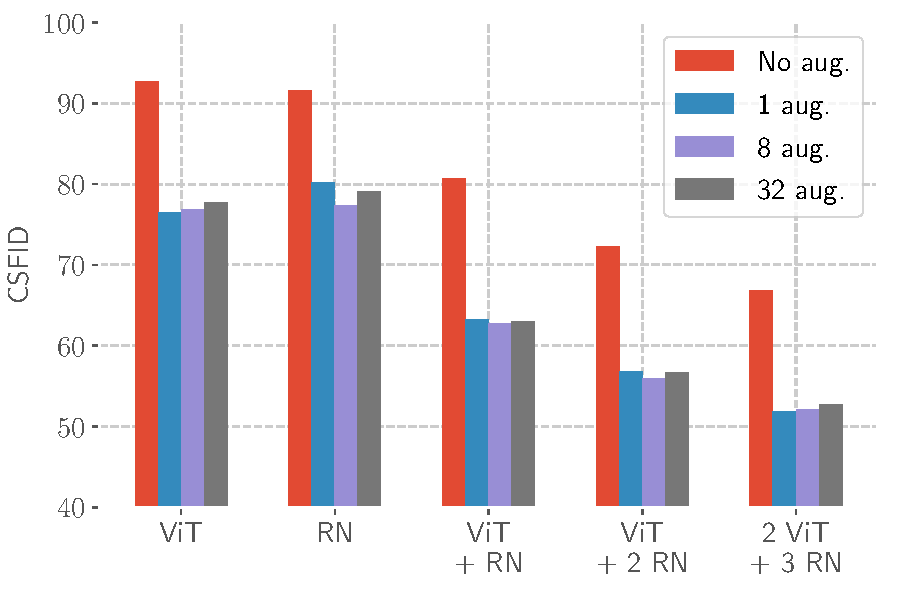
\includegraphics[width=.9\linewidth]{images/flexit/assets/naug_nnets.pdf}
    \caption{CSFID for different CLIP networks combinations and number of data augmentations options. Default setting: ViT+2RN.}
\label{fig:augs}
\end{figure}



We study how different choices of \ac{CLIP} image encoders impact the \ac{CSFID} score. 
Our default configuration involves two ResNet-based networks and one ViT-based network 
to embed the image in the \ac{CLIP} space. 
We experiment with a single ViT or ResNet, a combination of ViT with a single  ResNet,  
and also using all available pre-trained \ac{CLIP} networks, which comprises a ViT-B/16, a
 ViT-B/32, a ResNet50, ResNet50$\times$4 and ResNet50$\times$16,
  see~\citep{radford2021learning} for details on the modules.
For each \ac{CLIP} network configuration, we experiment with  either  not using data 
augmentation, or using $d \in\{ 1, 8, 32\}$ augmentations, as described in~\ref{sub_section:implementation_details}.
Each of the $N_\textrm{nets}$ \ac{CLIP} networks sees a different augmentation in each of 
the $N_\textrm{steps}$ optimization steps,  resulting in a total of
 $d \times N_\textrm{nets} \times N_\textrm{steps}$ augmentations of the input image.

From the results in Figure~\ref{fig:augs}, we see that while the  ViT and  ResNet 
embedding networks lead to similar results, they are complementary and combining them 
leads to a substantial improvement.  
Adding additional networks leads to further improvements.
%
Second, using data augmentation is very beneficial, and leads to a reduction in \ac{CSFID} 
of 10 or more points for all network configurations. 
Using more than one augmentation does not improve results substantially: it suffices 
to use a different augmentation for each network at each optimization step.
In our other experiments we use the three smallest (and fastest) \ac{CLIP} networks as our 
default setting.





In Table~\ref{table:runtime}, we show ablations for combining multiple \ac{CLIP} networks and using multiple data augmentations in the 
multimodal encoder. This table also reports the runtime needed for each algorithm, which plays a role in our choices.


\begin{table}[H]
\center
\begin{tabular}{lrrrrrr}
\toprule
 networks & d & \textbf{Acc.↑} &  \textbf{PIPS↓} &  \textbf{CSFID↓} &  \textbf{SFID↓} & \textbf{\thead{sec.\\ /im}} \\
 
\midrule
         ViT-B/32 & 0 & 9.4 &   21.8 &   92.7 &  7.4 & 27s   \\
         ViT-B/32 & 1 & 37.5 &   26.4 &   76.5 & 11.1 & 27s  \\
         ViT-B/32& 8 & 35.1 &   25.4 &   76.9 & 10.7 & 33s \\
         ViT-B/32& 32 & 35.5 &   25.0 &   77.7 & 10.8 & 53s \\
\midrule
        RN50x4 & 0 & 13.4 &   23.8 &   91.6 & 11.8 & 35s \\
         RN50x4& 1 & 32.5 &   27.4 &   80.2 & 13.7 & 35s  \\
         RN50x4& 8 & 31.0 &   25.2 &   77.3 & 12.3 & 53s \\
        RN50x4& 32 & 27.0 &   24.2 &   79.1 & 11.7 & 122s \\
\midrule

          2 nets & 0 & 23.0 &   22.8 &   80.7 &  9.5 & 39s \\
          2 nets & 1 & 50.6 &   26.4 &   63.2 &  8.9 & 39s \\
          2 nets & 8 & 47.8 &   24.9 &   62.7 &  8.4 & 64s \\
          2 nets & 32 & 47.4 &   24.2 &   62.9 &  8.1 & 160s \\
  \midrule
        3 nets & 0 & 30.4 &   22.5 &   72.2 &  8.3  & 45s\\
        3 nets& 1 & 54.9 &   26.0 &   56.7 &  6.7 & 45s \\
        \rowcolor{LightGrey}
        3 nets& 8 & 52.6 &   24.6 &   55.9 &  6.4 & 75s \\
        3 nets& 32 & 51.7 &   24.0 &   56.7 &  6.7 & 190s \\
        \midrule
         5 nets & 0 & 39.6 &   22.4 &   66.8 &  7.7 & 70s \\
        5 nets& 1 & 60.3 &   25.5 &   51.9 &  5.5 & 70s \\
        5 nets& 8 & 60.1 &   23.9 &   52.1 &  5.4 & 176s \\
        5 nets& 32 & 52.0 &   22.8 &   52.7 &  5.2 & 560s \\
        \bottomrule

\end{tabular}

\caption{\label{table:runtime} Ablation results for the multimodal encoder components. $d$ is the number of augmentations. 
$d=0$ means that the encoder takes the unchanged image as input; For $d=1$, the encoder takes only one (augmented image), 
which explains why the edit time is the same as $d=0$.
When considering $n$ \ac{CLIP} networks, we take the first $n$ elements in the following list: RN50x4, ViT-B/32, RN50, 
ViT-B/16, RN50x16. 
Our default configuration  is marked in light grey. 
Last column gives computation time per image in seconds.
}

\end{table}


\subsection{Image optimization space} 
We compare our choice of optimizing in the VQ-GAN latent space with using the latent
 spaces of StyleGAN2~\citep{karra2020stylegan2} and IC-GAN~\citep{casanova21nips}, as well as 
 optimizing directly in the pixel space.

IC-GAN  generates images similar to an input image, 
and uses  a latent variable to allow for variability in its output. 
IC-GAN is naturally conditioned on the SwaV embedding~\citep{caron20nips} of the input image
but does not offer direct  inference of the latents  for a given image. We thus take 
1,000 samples from the latent prior, and keep the one yielding minimal \ac{LPIPS} distance 
to the input image. We found that  optimization to further reduce the \ac{LPIPS}  \wrt the input image from this
 point on was not effective.

For StyleGAN2~\citep{karra2020stylegan2}, we use the same  network  pre-trained on ImageNet 
as we used for StyleCLIP.
To embed the evaluation images into this latent space, we first obtain an initial 
prediction of the vector with the e4e encoder~\citep{tov2021designing}, as in StyleCLIP, 
and then  perform an additional 1,000  optimization steps to better fit the input 
image, following the \ac{GAN} inversion procedure described in \cite{karra2019stylegan}.

Figure~\ref{fig:encoders} shows that using the VQ-GAN latent space allows 
to substantially decrease the  \ac{CSFID} score along the iterations, while only slightly 
increasing \ac{LPIPS}. 
Using the raw pixel space is not effective to decrease the \ac{CSFID}. 
IC-GAN has relatively good image synthesis abilities but it is hard to faithfully
 encode images in its latent space, yielding high \ac{LPIPS} scores above 50. 
The StyleGAN2 latent space ($\mathcal{W+}$) is bigger, allowing generated images to 
be closer to the input images; however its \ac{CSFID} scores are not competitive with the 
other approaches. Figures~\ref{fig:encoders2} visually illustrates these different behaviors.


\begin{figure}[H]
    \centering
    \vspace{-1cm}
    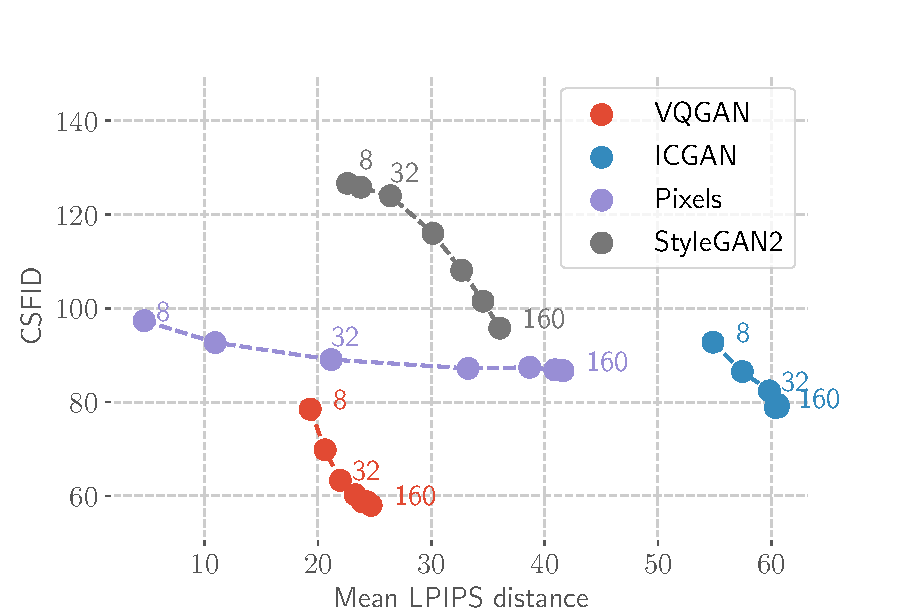
\includegraphics[width=.6\linewidth]{images/flexit/assets/encoder_evol.pdf}
    \caption{\ac{CSFID} and \ac{LPIPS} scores across iterations, using different latent spaces, or raw pixels, for optimization. 
    }
    \label{fig:encoders}
\end{figure}

\begin{figure}[H]
    \centering
    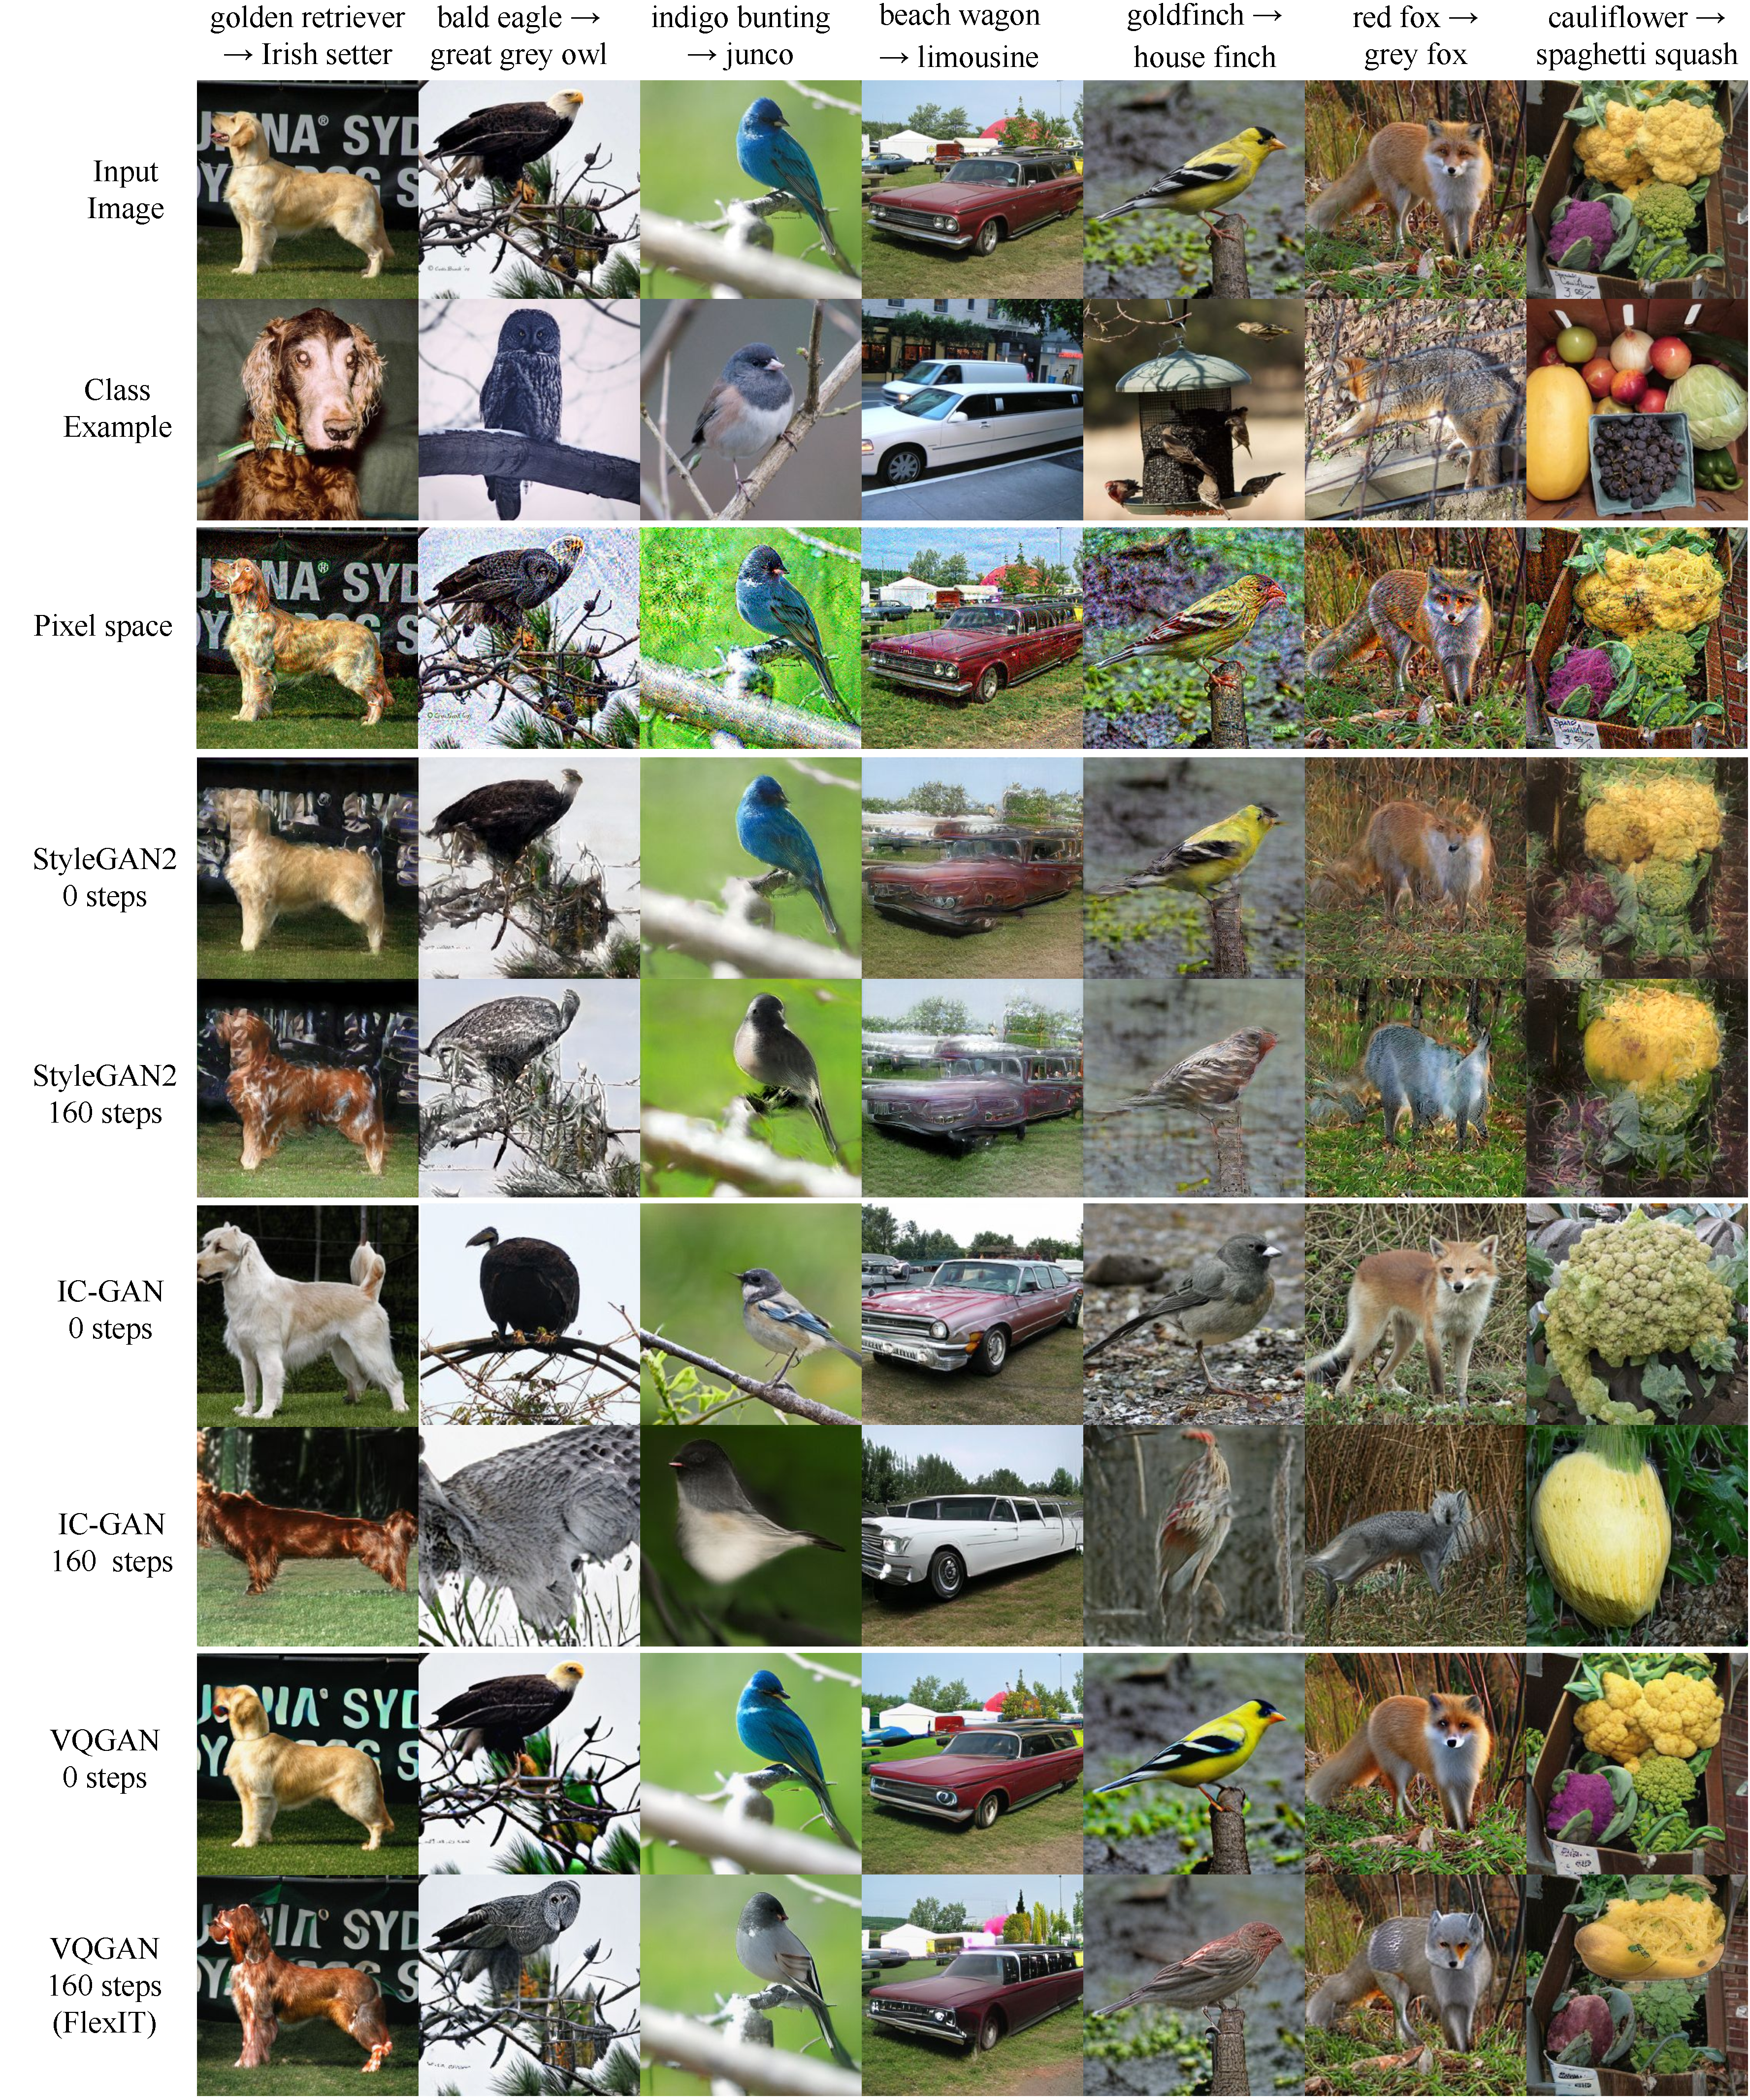
\includegraphics[width=0.9\linewidth]{images/flexit/assets/encoder2.pdf}
    \caption{Transformation examples with various backbones for the image latent space. For each latent space, 
    we show the initial image decoded from the initial point $z_0$, and the resulting image after 160 optimization steps. 
    At 0 steps, the three latent spaces differ substantially. The IC-GAN latent space 
    produces natural images that are far from the input image due to the limited generator capacity and the 
     smaller latent space size (2560 dim.). StyleGAN2 images preserve the input image 
    appearance with its larger size of its latent space $\mathcal{W+}$ (8192), but they contain
      unnatural artifacts \citep{tov2021designing}. 
     Our choice of VQ-GAN leads to good reconstruction results.
    After 160 steps of optimization, StyleGAN2 is unable to achieve natural edits while IC-GAN is 
    far away from the input images. The pixel-space method introduces high-frequency artifacts, 
    without substantially modifying semantic 
    image content, resembling adversarial examples. 
    VQ-GAN, which we use in FlexIT, achieves aesthetic edits while preserving the overall image appearance.
    }
\label{fig:encoders2}
\end{figure}





\subsection{Hyperparameter study}\label{hparam}

\begin{figure}[H]
    \centering
    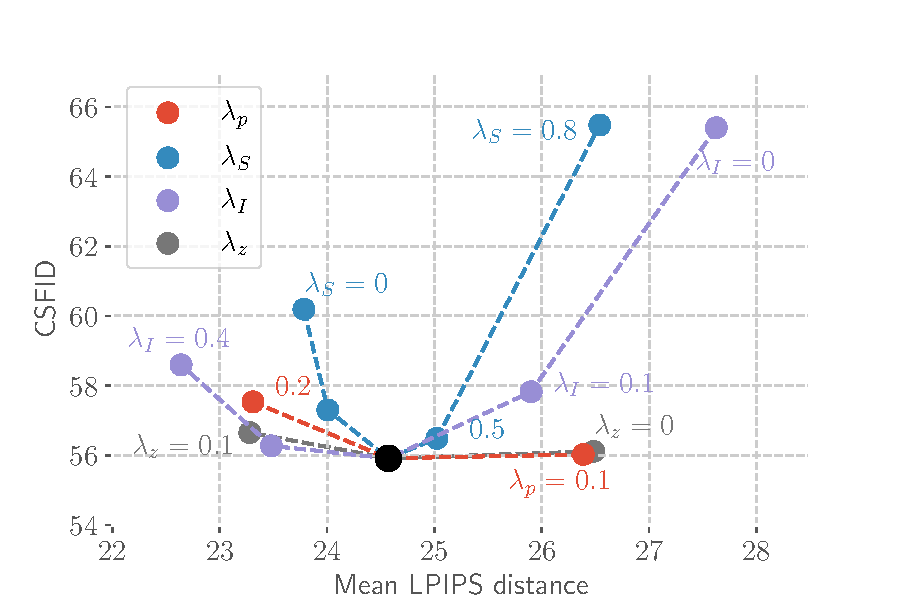
\includegraphics[width=0.8\linewidth]{images/flexit/assets/hparam_fig.pdf}
    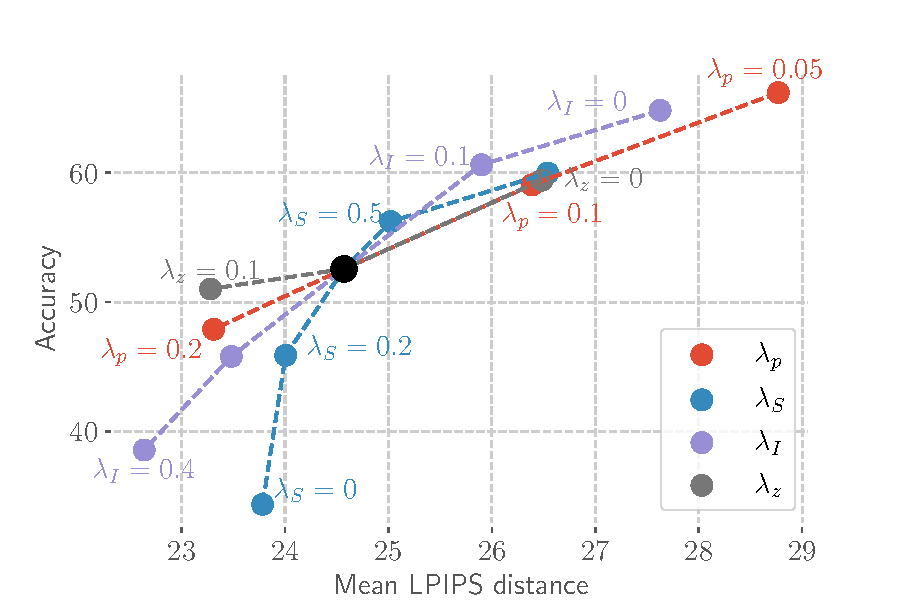
\includegraphics[width=0.8\linewidth]{images/flexit/assets/hparam_acc.pdf}
    \caption{Effect  on \ac{CSFID} and Accuracy of hyper-parameters;  default settings  represented by 
    the black dot, where all lines cross.}
\label{fig:hparam_csfid}
\end{figure}


In Figure~\ref{fig:hparam_csfid}, we illustrate the effect of our hyper-parameters on
 the \ac{LPIPS}, \ac{CSFID}, and Accuracy metrics. 
For the three regularization parameters $\lambda_p, \lambda_z, \lambda_I$, we observe
 that
(i) the \ac{LPIPS} distance with respect to the input image is smaller as the regularization 
gets stronger, as expected; 
(ii) less regularization allows more image modifications, yielding better accuracy
 scores, as illustrated in the bottom panel; 
(iii) there is a global minimum in \ac{CSFID} scores when we vary each hyper-parameter 
 independently (top panel). Regularization constraints are indeed useful to prevent
  inserting unnatural visual artifacts; however, too much regularization penalizes our 
  algorithm as the distribution of output images gets closer to the input distribution, 
  and thereby farther from the  target distribution.

The parameter $\lambda_S$, similarly to the regularization parameters, has a an optimal
 value which minimizes the \ac{CSFID}. It is beneficial to give a hint to the optimization 
 algorithm which semantic content should be changed, however focusing too much this 
 objective reduces image realism.

For our main experiments, we set our hyper-parameters to  minimize the \ac{CSFID} score on 
the development set. This is a natural choice given the convex shape of the \ac{CSFID} 
scores, whereas optimizing for accuracy  would   remove the regularizers which is 
detrimental for image quality.


\section{Limitations}

\begin{figure}[h]
    \center
    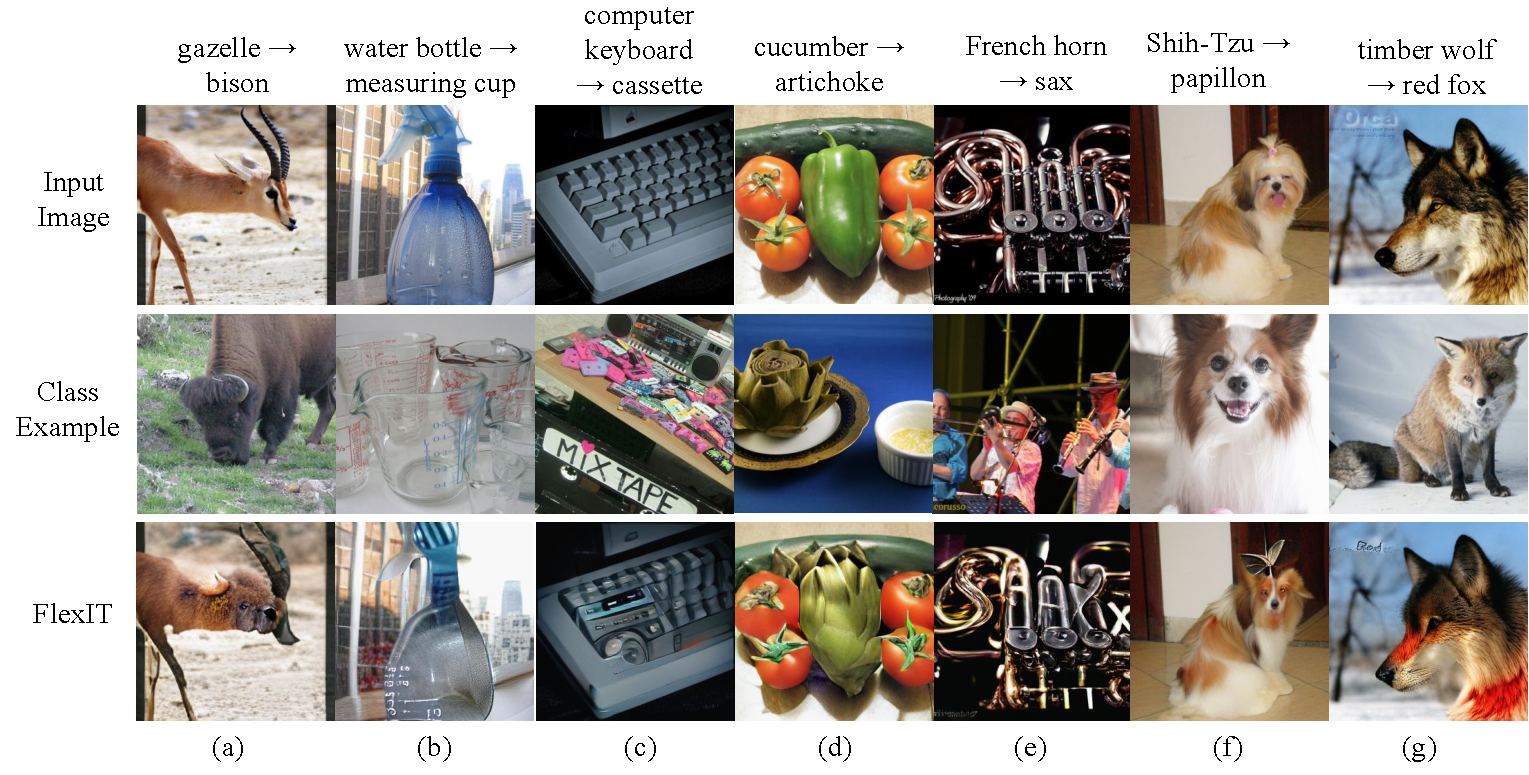
\includegraphics[width=\linewidth]{images/flexit/assets/failures.pdf}
    \caption{
    Representative failure cases of FlexIT. 
    Columns (a)--(c) illustrate a too strong regularization with respect to the initial image. 
    (d): the bell pepper was transformed instead of the cucumber, probably because the former is more centered, and has a better initial shape. 
    Columns (e)--(g) show failure cases related to the \ac{CLIP} embedding space. 
    (e): ``sax'' have been written in the image. 
    (f): a butterfly is synthesized on the head of the dog (\ac{CLIP} optimized for both the dog breed papillon and the insect papillon). 
    (g): saturated red was added to the image instead of the fox breed.
    }
\label{fig:failures}
\end{figure}

While our method  often offers compelling results, it can also fail in many cases, 
as shown in Figure~\ref{fig:failures}. While our choice of hyperparameters work well 
globally, specific images may respond poorly to the regularization parameters, as shown 
in the first three columns of Figure~\ref{fig:failures}. Our method is limited to the capacities 
of the multimodal embedding space \ac{CLIP}, which, although more semantic than the the pixel space, 
can still be prone to overfitting despite our regularizers, as shown in Figure~\ref{fig:failures} (e) 
and Figure~\ref{fig:visuresu} (last two columns). Moreover, because \ours depends on \ac{CLIP}, 
it could also inherit its biases,
such as misclassifying human faces into non-human or crime-related categories, and 
producing gender biased associations. Our editing method could reflect such biases if 
prompted transformations such as doctor $\rightarrow$ newscaster.

Our method 
works best for semantic translation when the input image provides guidance,
 but has difficulties synthesizing realistic novel objects from scratch. Other transformations 
 of interest could consider changing the 
action of a subject (person walking \vs  running), changing object attributes, 
adding or deleting objects, or consider more elaborate textual descriptions which 
require non-trivial grounding in the image (``change the color of car parked next to 
the bicycle.''). Importantly, progress in this direction will require to identify the 
right data and evaluation metrics. 




\section{Conclusion}

 We propose \ours, a novel method for semantic image translation.
 We also propose an evaluation protocol for semantic image translation, based on ImageNet,
 which we use to thoroughly evaluate our approach and its components.
 We have shown that with well-studied regularizers, we can give editing capabilities 
 to a non-generative model (the autoencoder of VQ-GAN). This allows us to circumvent the 
 problems inherent to \ac{GAN} inversion, as seen in Chapter~\ref{chapter:magec}.
 By relying on an autoencoder latent space, rather than specialized \ac{GAN} latent spaces,
 it can operate on a wide range of images. Using a general pre-trained multi-modal 
 embedding space provides  flexibility, giving 
 \ours the ability to process free-text transformation queries without training.

 However, because our image generator (the decoder of VQ-GAN) is not a generative model, 
 realistic edits are not guaranteed. Later and concurrent works to this paper focus greatly 
 on Diffusion Models. In  early works on editing with \ac{DDPM}s,~\citep{meng2022sdedit}, 
 for example, show that by modifying an image with strokes and then simply noising and denoising it (with the \ac{DDPM}),
 we can leverage the generative capacities of the \ac{DDPM} and turn the stroke into a realistic edit. 
 This easy inversion scheme, combined with using an actual generative prior, makes Diffusion Models 
 a perfect candidate for our work, not prone to the weaknesses of neither Chapter~\ref{chapter:magec}
 nor this chapter. In the next chapter, we will explore these models for the general task of 
 image inpainting.








\cleardoublepage
\let\leftmark=\oldleftmark

\acresetall
\chapter{GradPaint}
\label{chapter:gradpaint}

% \begin{chapabstract}
%     pass
    

% \end{chapabstract}
% \newpage

\minitoc
\chapterwithfigures{\nameref*{chapter:gradpaint}} \chapterwithtables{\nameref*{chapter:gradpaint}}

\ifthenelse{\boolean{skipGrad}}{\endinput}{}

\section{Introduction}

Inpainting consists in generating a missing part of a given image, given a binary mask 
indicating where the generation should take place. It is a fundamental task in computer
 vision, having obvious implications for image editing, image restoration, object 
 removal, and so on. Currently, state-of-the-art methods are generally based on 
 Generative Adversarial Networks (GANs) \cite{lama, zhao2021comodgan}, and consist 
 in explicitly training a model to reconstruct an image using self-generated masks.
  Although these methods often achieve reasonable results with standard metrics, 
  visual results tend to have obvious, unrealistic artifacts. Moreover, training 
  these models is accompanied with the difficulties of training instability inherent 
  with GANs as well as limitations on the diversity of the dataset distribution. 

Denoising diffusion probabilistic models (DDPMs) have recently gained massive attention,
 achieving high-resolution, photo-realistic and diverse image generation 
 \citep{dalle2, imagen, latentdiffusion, latentdiffusion2, guided-diffusion, glide}. In 
 terms of image generation, these models are on par or better than GANs even for 
 constrained datasets like faces \cite{latentdiffusion}; and largely surpass them for 
 diverse datasets like ImageNet \cite{glide, latentdiffusion}. Furthermore, 
 recent models trained on large-scale datasets 
 \cite{imagen, dalle2, glide, makeascene, latentdiffusion} have given rise to 
 high-quality and flexible text-conditioned image generation, allowing users to 
 generate astonishingly imaginative or artistic high-resolution images \cite{artcomp}. 
 It is thus highly enticing to be able to use these pretrained models directly for
  downstream tasks, rather than re-training a new model from scratch. Here, we focus 
  on the particular downstream task of inpainting.

There has been limited work in using pre-trained diffusion models for this task, and 
the typical approach \cite{repaint, meng2022sdedit, glide} is to guide the generative 
model by replacing values of the intermediate noise map with noised pixels of the input 
image outside the inpainting mask, based on the hope that the denoising process inside 
the inpainting mask will progressively be biased towards image parts that blend 
naturally with the known surrounding context.
%iteratively combining a noisy masked ground-truth part with the masked generated part and denoising this constructed latent map with the pre-trained model. The intuition is that these combined noise maps, while corresponding to incoherent concepts at first, will gradually merge together into a harmonious image thanks to the denoising process \cite{meng2022sdedit}.
However, this strategy often produces unsatisfying results, which we believe is due to
 the diffusion model being strongly conditioned on the initial noise
  map \cite{optimaltransport}, therefore having difficulties harmonizing the generation
   when the initial random latent map is too mismatched with the input image.


% \matt{Je trouve que la suite et fin de l'intro est bien mais trop narative linéaire. A discuter mais peut etre essaie de rester un peu plus general pour ensuite rassembler en 2 bullets les main contrib algo/expe ou tu pourra pour chacune entrer plus dans le détail technique.}
% This key observation - that the initial latent map strongly conditions success or failure of inpainting - is the motivation for our work. We propose to address this problem with direct optimization of the latent map. 
% We add a step of gradient descent at every iteration of the denoising process to directly optimize the noise vector, with the explicit objective of harmonizing the generated part with the masked input image. We leverage the model's prediction of the denoised image at every time step, and calculate how well this denoised image matches our input image. This is measured using a masked L2 loss as well as an \emph{alignement loss} which measures smoothness at the frontier of the merged image parts. The combined loss is backpropaged directly into the diffusion model itself, and its gradient is used to improve the noise map at each step of the denoising process. We also study the best way to combine the masked generated part with the unmasked input part, and propose a general protocol for inpainting with diffusion models.


In this paper, we propose a new strategy for guiding pre-trained diffusion models
to better perform inpainting tasks. Our method, dubbed GradPaint, is optimizing the
 diffusion process by better harmonizing generated content inside the inpainting mask.
  This guides the generation at every single step of the denoising process towards a
   more harmonized final image.  Our method aims to minimize or even eliminate all the 
   artifacts and inconsistencies that generally persist on the images due to the masked
    regions.
We propose a training-free algorithm which is advantageous because (i) there is no need 
to train a inpainting-specialized model whenever a new model is available, and (ii) 
training-based methods must chose a mask distribution to train on, to which training-free
 methods are agnostic. We perform an extensive evaluation on various datasets, 
 including  CelebA-HQ\cite{celebahq}, FFHQ\cite{ffhq}, ImageNet\cite{imagenet},
  Places2\cite{zhou2017places}, and COCO\cite{cocodataset}. 

Our main contributions can be summed up as:

\begin{itemize}
    \item We propose a novel training-free algorithm to the denoising scheduling of 
    diffusion models for the specific task of inpainting. We improve this inpainting
     mechanism with the explicit goal of harmonizing the generated parts with the current context. Specifically, we use a custom \textit{alignment loss} and leverage the intrinsic nature of diffusion models through which we back-propagate and calculate a gradient to optimize our loss. 

    \item We show that our method generalizes well to a variety of datasets and 
    pre-trained models, including latent-diffusion models. We show that our method 
    improves baseline methods and is even on par with equivalent models trained 
    specifically for the task of inpainting.
\end{itemize}

% We show that our simple modification to the denoising scheduling yields a massive improvement in both qualitative and quantitative results.  We validate our results on a variety of pre-trained conditional and unconditional models, including latent diffusion models. We improve baseline methods on various datasets, including CelebA-HQ\cite{celebahq}, FFHQ\cite{ffhq}, ImageNet\cite{imagenet}, Places\cite{zhou2017places}, and COCO\cite{cocodataset} and show that our method improves baseline methods and is even on par with equivalent models trained specifically for inpainting. 


\section{Related Work}



% Historically, the inpainting task aimed at replacing corrupted parts in images with more plausible image parts, so the evaluation criterion was naturally a distance metric with respect to the uncorrupted or unmasked image. More recently, generative models have became able to synthetize convincing images for datasets with diverse images, allowing to fill in larger regions when editing images. With larger inpainting masks, generative models have more freedom to inpaint details that are different from the ground truth value, as long as the resulting output looks realistic. Therefore, \textit{image realism}, as measured by the FID score \cite{heusel2017gans} for instance is the most important metric to compare 

%\matt{general comment sur inpainting  different methods. et discuter le fait que historiquement le critere d'éval c'est retrouver au mieux l'image originale alors que dans le contexte recent generatif avec des masquages tres important le critere le plus important pourrait être la plausibilité }


\subsection{Inpainting}

Historically, inpainting was aimed at recovering small corruption errors in images and 
was addressed with matching or ``borrowing" local color and texture around the masked
 region \cite{poisson, patch_based}. Evaluation consisted in calculating a distance
  metric with respect to the unmasked image. More recently, generative models have 
  become capable of synthesizing realistic and diverse images, allowing the use of much
   larger masks when inpainting images. Generative models thus have more freedom 
   to ``imagine" a wide range of possibilities much different from the reference image,
    which is satisfactory (and oftentimes desired) so long as the resulting output looks
     realistic. 

In recent years, inpainting has been primarily addressed with training deep 
encoder-decoder convolutional networks from scratch, often using a 
GAN\cite{goodfellowgans} loss to encourage plausibility. Most recent work consists in 
improving the typical convolutional architecture in the encoder and/or decoder to better
 leverage structural or textural information from the surrounding regions 
 \cite{lama, hong2019deep, yu2020region, hukkelaas2020image, yang2020learning, zhu2021image, liu2018image, ma2022regionwise, zheng2022cm}. 
 \cite{li2020recurrent} proposes a progressive inpainting scheme which iteratively 
 fills in the mask by using surrounding information in the deep feature space.  
 \cite{xiong2019foreground, liao2020guidance} propose a framework to locate and 
 leverage semantic information.


% pre-trained models !??

In another line of work similar to ours, image completion is effectuated with the 
help of existing priors not specifically trained for the task. \cite{ulyanov2018deep} 
trains a randomly initialized convolutional network to generate the input image, 
stopping training before overfitting occurs. \cite{psp, zhao2021comodgan, glean} 
utilize powerful pre-trained decoders like StyleGAN2\cite{stylegan2} and only train
 encoders to map the input image into the latent space of the decoder, which can produce
  more realistic results if the input image fits well to the distrubtion of the
   pre-trained decoder. 




\begin{figure*}[h]
  \centering
    \includegraphics[width=\textwidth]{images/gradpaint/method.pdf}
    \caption{GradPaint method overview. We propose to modify one step of the DDPM denoising process with a gradient descent update on $x_t$ to better match the masked input image, in turn producing a better matched noise map $x_{t-1}$ for the next step. This improvement in the DDPM noise prediction thus allows for better fitting intermediate noise map predictions $x_t$ earlier in the DDPM denoising process, which ultimately produces a successful final inpainted image $x_0$.}
    \label{fig:method}
\end{figure*}

%\matt{etoffer dire que c'est une etape des DDPM sampling modifié, qui compose avec la pred et le mask pour calculer un gradient dedie et le recombiner apres une interpolation pour calculer le next bruit ... Biensur la prediction direct n'est pas très bonne, recombinée avec l'image maskée cest mieux mais surtout ca permet de calculer des gradient sur tout xt utiles pour la prochaine reconstruction...}

\subsection{Diffusion models}

Diffusion models are becoming state-of the art methods for generation tasks on many 
modalities, like images, videos, speech and text. Their excellent scaling behavior makes 
them a model of choice for training on large and diverse data, compared to GANs which 
still suffer from mode collapse and training instabilities. They can also be conditioned
 on various input data: for the specific task of inpainting, the input image and mask 
 can be given as additional input to train a conditional diffusion model specialized on
  the inpainting task, as done in \cite{saharia2022palette}.

However, due to the computational cost of training generative models, it is appealing 
to find adaptation algorithms for downstream tasks without fine-tuning, especially for
 the task of inpainting which bears a lot of similarities with the unconditional 
 generation task. \cite{latentdiffusion, glide, song2021scorebased} propose to adapt
  pre-trained diffusion models to inpainting by injecting a guiding mechanism in the 
  generative process, a strategy which we build upon in this paper. \cite{repaint} also
   proposes to take advantage of pre-trained diffusion models with cycles of denoising 
   and renoising operations, which we found computationally very expensive. Finally, 
   in a parallel line of work most similar to ours, \cite{mcg} similarly propose to
    guide the generation using the gradient of a ``manifold constraint", but they do 
    not use a custom loss nor do they apply optimization to the entirety of the 
    intermediate noise maps.


\documentclass[main_for_review.tex]{subfiles}

\begin{document}

\section{GradPaint Method}

%Given an input image $x_0$ masked out by a binary mask $m$, our goal is to generate a realistic image $x$ such that $x \odot (1-m) = x_0 \odot (1-m)$ and $x \odot m$ is generated.

% At a given timestep $t$ during the diffusion process, we use our pre-trained diffusion model to predict $\hat{x}_0$.

\subsection{Background}
\label{background}

Denoising diffusion probabilistic models \cite{ho2020denoising} is a class of generative models trained with the following image denoising objective:

\begin{equation}
    \mathcal{L} = \displaystyle \mathbb{E}_{\x_0, t, \epsilon} \Vert \epsilon - \epsilon_\theta(\x_t, t) \Vert_2^2,
\end{equation}
where $\epsilon_\theta$ is a noise estimator network trained to predict the noise $\epsilon \sim \gaussian$  mixed with an input image $\x_0$ in the following way: $\x_t = \sqrt{\alpha_t} \x_0 +  \sqrt{1 - \alpha_t} \epsilon$. This training is performed for different values of the mixing coefficient $\alpha_t$, monotonically decreasing from $\alpha_0 = 1$ (no noise) to $\alpha_T \simeq 0$ (almost pure noise) for a large integer $T$.

At inference time, a new sample from the training distribution can be obtained by starting from random Gaussian noise $\mathbf{x}_T \sim \mathcal{N}(\mathbf{0}, \mathbf{I})$, and iteratively refining it with the noise estimator network with the following equations, called \textit{DDPM sampling equations} \cite{ho2020denoising}:

$x$ and $\x$
\begin{align*}
\hat{\x}_0 & = \frac{1}{\sqrt{\alpha_t}}(\x_t - \sqrt{1 - \alpha_t} \cdot \epsilon_\theta(\x_t, t)), \numberthis \label{eq:ddpm1}\\
%\x_{t-1} & = \sqrt{\alpha_{t-1}} \hat{\x}_0 + \sqrt{1 - \alpha_{t-1} - \sigma_t^2} \cdot \x_t + \sigma_t \boldsymbol{z}, \numberthis
\x_{t-1} & = \frac{(\alpha_{t-1}-\alpha_t) \sqrt{\alpha_{t-1}}}{\alpha_{t-1}(1 - \alpha_t)} \hat{\x}_0 + \frac{(1-\alpha_{t-1})\sqrt{\alpha_t}}{(1 - \alpha_t)\sqrt{\alpha_{t-1}}} \x_t + \sigma \boldsymbol{z},
\end{align*}
where $t$ goes from $T$ to $0$, 
$\sigma_t$ is a variance parameter, and $z \sim \gaussian$.

This iterative refinement can be ``guided" to impose constraints on the generated sample $\x_0$. In the case of inpainting, the aim is that the generated image exactly matches the input image outside a given inpainting region. The variable $\hat{\x}_0$, available at each timestep, represents the model's current estimation of what the denoised image will look at the end. For instance, \cite{glide} applies a maskwise correction on $\hat{\x}_0$ at each timestep:
\begin{equation}
\hat{\x}_0' = M \odot \hat{\x}_0 + (1 - M) \odot I,
\end{equation}
where $I$ is the input image and $M$ is a binary image mask equal to 1 in the image regions that must be inpainted, 0 otherwise. The update rule for $\x_{t-1}$ is then adapted to use $\hat{\x}_0'$ instead of $\hat{\x}_0$ in \autoref{eq:ddpm1}. This correction progressively biases the diffusion model to exactly match $I$ outside the inpainting mask $M$. In the remaining of the paper, we refer to this method as \textit{combine-image} since it combines the images $\hat{\x}_0$ and $I$ before interpolating with $\x_t$.

Alternatively, \cite{song2021scorebased, latentdiffusion, repaint} propose to directly correct $\x_{t-1}$ by replacing regions outside $M$ with the noised regions of the input image $I$:
\begin{equation}
\x_{t-1}' = M \odot \x_{t-1} + (1-M) \odot (\sqrt{\alpha_{t-1}} I +  \sqrt{1 - \alpha_{t-1}} \epsilon),
\end{equation}
where $\epsilon \sim \gaussian$ is resampled at each step. This $\x_{t-1}'$ is then used as input for the next denoising step instead of $\x_{t-1}$. We will refer to this method as \textit{combine-noisy} since it combines $\x_{t-1}$ inside the mask with ground truth (noised) pixel values outside the mask.


\subsection{GradPaint framework}


%MOVE FIG PAR MATT 



Our strategy is built upon the \textit{combine-image} zero-shot inpainting method presented in \S\ref{background}. Our key observation is that the most asthetically-pleasing inpainting results are obtained when the collage $M \odot \hat{x}_0 + (1-M) \odot I$ is coherent right from the beginning of the generation process. When this is not the case, there is a mismatch between the model's estimation in the inpainting region and the known regions of input image $I$. This mismatch is generally present from the beginning and is not fully corrected during the denoising generation process. 
%\matt{FAIRE REF A LA FIG 2}

To enforce harmonization between the inpainted region and known regions of the input image, we introduce the \textit{GradPaint update}. An overview of our method is presented in Fig.~\ref{fig:method}.
At each denoising step, the variable $\x_t$ is updated so that (i) $\hat{x}_0$ matches well known regions of $I$ outside the mask; and (ii) the collage $M \odot \hat{x}_0 + (1-M) \odot I$ does not present any discontinuity due to the copy-paste operation. This update consists in a one-step gradient descent update from two loss terms corresponding to the two objectives aforementioned. %\matt{FAIRE REF A LA FIG 2 pb corrigé}


%The success of the harmonization is calculated with a custom loss $l(x_0, \hat{x}_0, m)$, which we will describe in detail. 

%The losses we use to encourage image harmonization are detailed below.

%\matt{pourquoi on passe de M à m ? mettre m partour ?}
Given a binary mask $M \in \mathbb{R}^{n \times n}$ and $\odot$ denoting the element-wise product, we define our losses as follows:
%$I_1 \in \mathbb{R}^{n \times n}$ and $I_2 \in \mathbb{R}^{n \times n}$, 

\noindent \textbf{Masked MSE loss.} The first loss term is a mean squared error term outside the inpainting mask $(1 - M)$, taking as reference known regions of the input image:
\begin{equation}
    \mathcal{L}_{mse}(I_1, I_2, M) = \frac{1}{n^2}\Vert I_1 \odot (1 - M) - I_2 \odot (1 - M) \Vert_2^2. 
\end{equation}
%\noindent \textbf{Masked LPIPS loss}:\\
%Similarly, the LPIPS loss will only be applied a masked region.
%\begin{equation}
%    LPIPS_{mask}(I_1, I_2, m) = LPIPS(I_1 \odot (1 - m), I_2 \odot (1 - m)) 
%\end{equation}
\noindent \textbf{Alignment loss.} The ``alignment loss" $al(I, M)$ measures the smoothness of image $I$ on the boundaries of the inpainting mask $M$. It is defined as follows:
\vspace*{-.1cm}\begin{equation}
    al(I, M) \hspace{-0.1cm}=  \hspace{-0.1cm} \frac{1}{n^2}\Vert D_x I \odot D_x (1 - M) +D_y I \odot D_y (1 - M) \Vert_2^2, 
\end{equation}
where $D_x$ and $D_y$ are the normalized image gradients:

%\noindent Given an image $I$, we compute its normalized image gradient:
% $$||\nabla I||_2 \in \mathbb{R}^{(n, n, 2)}$$


\begingroup\makeatletter\def\f@size{9}\check@mathfonts
\def\maketag@@@#1{\hbox{\m@th\large\normalfont#1}}%
\begin{align*}
 \begin{bmatrix}
D_x I \\
\vspace{-0.2cm}\\
D_y I \\
\end{bmatrix}_{(i, j)}
&= 
\begin{cases}
\dfrac{\nabla I_{(i, j)}}{||\nabla I_{(i, j)}||_2} , & { \text{if } ||\nabla I||_{(i, j)} > 0} \vspace{0.1cm} \numberthis \\
[0 \quad 0]^T
, & \text{else}
\end{cases} \\
%=&
%\begin{cases}
%\dfrac{1}{\sqrt{{\partial_x I_{(i, j)}}^2 + {\partial_y I_{(i, j)}}}} \times
%\begin{bmatrix}
%\partial_x I \\
%\vspace{-0.2cm}\\
%\partial_y I \\
%\end{bmatrix}_{(i, j)}, & \text{if } ||\nabla I||_{(i, j)} > 0 \\
%0, & \text{else}
%\end{cases}
\end{align*}\endgroup

% \in \mathbb{R}^{(2, n, n)}

% \[
%     f(x)= 
% \begin{cases}
%     \frac{x^2-x}{x},& \text{if } x\geq 1\\
%     0,              & \text{otherwise}
% \end{cases}
% \]


\noindent with $\nabla I = [\partial_x I \; \partial_y I]^T$ is the vector of gradients of $I$ in the $x$ and $y$ directions respectively. 
When we minimize this loss, we aim to achieve the smoothest transition possible in the image $I$ along the direction where $M$ changes values. 
Since this loss $al(I, M)$  is defined for an image with only one color channel, we simply define the total alignment loss $\mathcal{L}_{al}$ as the average loss over the three color channels for a regular RGB image.


\noindent \textbf{GradPaint ~Update.} Our total loss is defined as:

\begin{equation}
\mathcal{L} = \mathcal{L}_{mse} + \lambda_{al} \mathcal{L}_{al},
\end{equation}
with $\lambda_{al}$ being a hyperparameter controlling the relative strength of the alignment loss compared to the MSE loss.

%\begin{align} 
%\begin{split}
%l(x_0, \hat{x}_0, m) = & \lambda_{mse} \times mse_{mask}(x_0, \hat{x}_0, m) + \\
%& \lambda_{lpips}  \times LPIPS_{mask}(x_0, \hat{x}_0, m) + \\
%& \lambda_{align}  \times \frac{1}{3} \sum_{ch=1}^3 align(x_{paste}^{ch}, m)
%\end{split}
%\end{align}

%where 

%$$
%x_{paste}^{ch} = (x_0 \odot m + \hat{x}_0 \odot (1 - m))^{ch}
%$$

%\noindent with $ch$ a channel in the $RGB$ space.

At each step in the denoising process, we compute $\x_{t-1}$ as a function of $\x_t$ as in the \textit{combine-image} method. In between each step, we update the variable $\x_{t-1}$ with the normalized gradient of our total loss:

\begin{equation}
\x_{t-1}' = \x_{t-1} - \alpha \frac{\nabla_{\x_t}\mathcal{L}(x_0, \hat{x}_0, M)}{\Vert \nabla_{\x_t}\mathcal{L}(x_0, \hat{x}_0, M) \Vert_2},
\end{equation}
with $\alpha$ being a fixed learning rate.



Backpropagating through the diffusion model itself until variable $\x_t$ is a crucial element of our method. Since $\x_t$ is updated to produce a better estimation $\hat{\x}_0$ when processed by the diffusion model, this property will also transfer to $\x_{t-1}$ which is, at each step, very close to $\x_t$.



%Our three losses encourage the predicted image $\hat{x}_0$ to be as close as possible to the original image $x_0$. 

%We perform our gradient-guided inpainting by first modifying $x_t$ in the direction minimizing this harmonization loss:

%\begin{equation}
%    x_t' = x_t - \alpha \nabla_{x_t}l(x_0, \hat{x}_0, m)
%\end{equation}

%We integrate the known information of $x_0$ directly by inserting it in $\hat{x}_0$:

%\begin{equation}
%    \hat{x}_0' = \hat{x}_0 \odot m + x_0 \odot (1-m)
%\end{equation}

%Finally, we perform a diffusion step by applying the posterior $q(x_{t-1} | x_{t}', \hat{x_{0}}')$.

%We should note that without guiding $x_t$ to $x_t'$, this method is equivalent to \flag{GLIDE's method}. We should also note that this method can be applied on top of any implicit inpainting method for diffusion models, notably \flag{repaint, latent diffusion...}. 

%At every step in the denoising process, we tweak $x_t$ via a step of gradient descent to create a more harmonized image when denoised and merged with $x_0$ along $m$. 

%too algorithmic; just take the gradient. %https://en.wikipedia.org/wiki/Image_gradient

\subsection{Visualizations}

\noindent \textbf{Harmonization.} The effect of the GradPaint update is illustrated in Fig.~\ref{fig:intuition}, 
which shows the intermediate DDPM predictions for $\hat{\x}_0$ and $\hat{\x}_0'$ at various timesteps. We 
compare GradPaint with the \textit{combine-noisy} and \textit{combine-image} methods presented in \S\ref{background}, where all three methods share the same DDPM model, parameters and initial noise maps.
These baseline approaches require more steps to integrate the information from the input image, at which point it is often ``too late" to construct a harmonized image - misalignment between the generation and the input image can no longer be corrected. In contrast, for GradPaint, the optimization step on $\x_t$ quickly pushes the merged image $\hat{\x}_0'$ to harmonizes well with the masked input image $\x_0$, producing an inpainting result without alignment artifacts.

 %Our method immediately guides the generation in the right direction, harmonizing the merged prediction at every timestep which in turn allows the DDPM to correct misalignment errors.
  

\begin{figure}[htbp]
  \centering
    \includegraphics[width=\linewidth]{images/gradpaint/intuition.pdf}
    \caption{DDPM predictions at different stages (indicated in $\%$) of the denoising process. We compare two baselines (a) and (b) with GradPaint (the two last rows). GradPaint better harmonizes regions inside and outside the inpainting mask right from the beginning of the denoising process.}
    \label{fig:intuition}
\end{figure}

\noindent \textbf{Gradient visualization.} The two separate components of our loss have different effects on $\nabla{\x_t}$, as we can see in Fig.~\ref{fig:loss_intuition-grad}.  While the gradient of the masked MSE loss remains active throughout the denoising process, the gradient of the alignment loss becomes obsolete about halfway-through, thereafter only concentrating in a few local points in $\x_t$. The gradient of the alignment loss has a concentrated effect on the borders of the mask, but also affects the entire noise map $\x_t$ globally, while the masked MSE loss has a much stronger effect in the unmasked region. The alignment loss encourages smoother and more gradual transitions in the final generation, as can be seen with the background in Fig.~\ref{fig:loss_intuition-int}. 




%putting the figure here so that it appears correctly
\begin{figure*}[htbp]
  \begin{subfigure}[b]{0.50\linewidth}
    \includegraphics[width=\linewidth]{images/gradpaint/losses2.pdf}
    \caption{Gradient magnitude of different components of our losses with regards to $x_t$. The alignment loss has a concentrated effect at the border and a more global effect compared to the masked MSE loss, but dies out more quickly when it concentrates in a few local spots.}
    \label{fig:loss_intuition-grad}
  \end{subfigure}
  \hfill %%
  \hspace{0.3cm}
  \begin{subfigure}[b]{0.45\linewidth}
  \centering
    \includegraphics[width=0.8\linewidth]{images/gradpaint/losses1.pdf}
    \caption{Intermediate DDPM predictions with GradPaint using separate components of our loss. The alignment loss encourages smooth and coherent transitions, as can be seen with the homologous background.}
    \label{fig:loss_intuition-int}
  \end{subfigure}
  \caption{Effect of separate components of our loss on the intermediate predictions of the DDPM model and their corresponding gradients. Noise maps are initialized identically.}
  \label{fig:loss_intuition}
\end{figure*}




\end{document}



\documentclass[main_for_review.tex]{subfiles}


\begin{document}

\section{Experimental Results}
%In this section, we describe our experimental setup to compare different algorithms on the inpainting task, and then expose qualitative and quantitative results.
%\subsection{Experiment setup}

\noindent \textbf{Evaluation protocol.} Given an image, the aim is to perform inpainting inside a random mask generated with the mask generator from \cite{lama}. We choose to only evaluate on the difficult and more realistic \textit{thick} masks, although the other settings can be found in the appendix. For a set of images inpainted with a given method, we compute two core metrics that encapsulate the challenges of inpainting: the LPIPS distance \cite{zhanglpips2018} between the inpainted image and the (unmasked) input image which measures the extent to which we correctly recover the masked regions, and the FID score \cite{heusel2017gans} which measures the realism of output images. The primary requirement is that inpainted images should look as natural as possible, hence having the smallest possible FID score. For LPIPS distances, an inpainting result closer to the reference image is generally better, although realistic images further away from the reference image can also be satisfactory, especially for large masks. We evaluate algorithms on five datasets: FFHQ, CelebaHQ, ImageNet, Places2 and COCO. For evaluation on FFHQ, we use CelebaHQ pre-trained models, and vice-versa. Remark that this is a more difficult evaluation setting than typically performed. For the pre-trained Places2 model, we use the validation set of Places2 for evalution. For inpainting on ImageNet, we use class-conditional models, and for COCO, we use image captions as conditioning text information to the diffusion model. On each dataset and each mask domain, metrics are computed using a set of 5000 images.\\
 \textbf{Pre-trained models and implementation details.} We primarily use diffusion models from guided diffusion \cite{guided-diffusion} \footnote{available at \url{https://github.com/openai/guided-diffusion/}}, which operates on images of size $256\times256$. We also experiment with latent diffusion models \cite{latentdiffusion}, which also operate on $256\times256$ images, but where images are edited in a latent space with spatial dimensions of $64\times64$.
For text-conditional models, we use Stable Diffusion. For our GradPaint method, we use a default number of 100 steps for DDPM sampling; the loss is computed with $\lambda_{al} =400$ during the first 45 steps of decoding (and disabled afterwards following our observations shown in \ref{fig:loss_intuition-grad}). The gradient is updated with a fixed learning rate of $0.005$.

\noindent \textbf{Baselines and other methods} We compute the best and worst possible LPIPS and FID scores with two trivial measures: the \textit{COPY} oracle measure, which simply copies the (unmasked) input image, gives an LPIPS score of $0$ and a lower bound on possible FID scores; and the \textit{GREYFILL} measure, which simply fills the region to be inpainted with uniform grey. Without gradient-based optimization, our method is equivalent to the \textit{combine-image} baseline for image inpainting, which we evaluate in our experiments along with its \textit{combine-noisy} variant. Apart from these three closely related methods, we compare against the following state-of-the-art inpainting methods:  LaMa\cite{lama}, a GAN-based method trained for inpainting; Palette \cite{saharia2022palette}, also trained for inpainting but with diffusion models, RePaint \cite{repaint}, another training-free inpainting algorithm that is much more computationally expensive, and finally MCG\cite{mcg}, a parallel line of work to ours which is similarly training-free but with a different optimization scheme. 


\subsection{Quantitative results}


\begin{table}[t]
\small
\begin{tabular}{|l|c|c|c|c|}
\hline
\multicolumn{1}{|r|}{Dataset} &
  \multicolumn{2}{c|}{FFHQ} &
  \multicolumn{2}{c|}{CelebaHQ} \\ \hline
%\multicolumn{1}{|r|}{Masks} &
  %\multicolumn{2}{c|}{Thin} &
  %\multicolumn{2}{c|}{Medium} &
  %\multicolumn{2}{c|}{Thick} &
  %\multicolumn{2}{c|}{Thin} &
  %\multicolumn{2}{c|}{Medium} &
  %\multicolumn{2}{c|}{Thick} \\ \hline

\multicolumn{1}{|r|}{Metrics} &
  \multicolumn{1}{c|}{FID$\downarrow$} &
  \multicolumn{1}{c|}{LPIPS$\downarrow$} &
  \multicolumn{1}{c|}{FID$\downarrow$} &
  \multicolumn{1}{c|}{LPIPS$\downarrow$} \\
   % & LPIPS$\downarrow$ & FID$\downarrow$ & LPIPS$\downarrow$ \\
%\multicolumn{1}{|c|}{Metrics} &
  %\multicolumn{1}{c|}{FID$\downarrow$} &
  %\multicolumn{1}{c|}{LPIPS$\downarrow$} &
  %\multicolumn{1}{c|}{FID$\downarrow$} &
  %\multicolumn{1}{c|}{LPIPS$\downarrow$} &
  %\multicolumn{1}{|c|}{FID$\downarrow$} &
  %\multicolumn{1}{|c|}{LPIPS$\downarrow$} &
  %\multicolumn{1}{c|}{FID$\downarrow$} &
  %\multicolumn{1}{c|}{LPIPS$\downarrow$} &
  %\multicolumn{1}{c|}{FID$\downarrow$} &
  %\multicolumn{1}{c|}{LPIPS$\downarrow$} &
  %\multicolumn{1}{c|}{FID$\downarrow$} &
  % \multicolumn{1}{c|}{LPIPS$\downarrow$} \\ 
  \hline %\hhline{|=|=|=|=|=|=|=|=|=|=|=|=|=|}
  \rowcolor[gray]{0.7}
COPY (oracle) &
  %\multicolumn{1}{c|}{4.29} &
  %\multicolumn{1}{c|}{0} &
  %\multicolumn{1}{c|}{4.29} &
  %\multicolumn{1}{c|}{0} &
  4.29 & 0
  %\multicolumn{1}{c|}{3.01} &
  %\multicolumn{1}{c|}{0} &
  %\multicolumn{1}{c|}{3.01} &
  %\multicolumn{1}{c|}{0} &
  & 3.01 & 0 \\ \hline
GREYFILL &
  %\multicolumn{1}{c|}{154.6} &
  %\multicolumn{1}{c|}{0.353} &
  %\multicolumn{1}{c|}{98.75} &
  %\multicolumn{1}{c|}{0.250} &
  78.08 &
  0.257
  &
  %\multicolumn{1}{c|}{173.65} &
  %\multicolumn{1}{c|}{0.3770} &
  %\multicolumn{1}{c|}{124.32} &
  %\multicolumn{1}{c|}{0.2631} &
  96.41 &
  0.264
   \\ \Xhline{4\arrayrulewidth}
LaMa&
  %\multicolumn{1}{c|}{\textbf{6.22}} &
  %\multicolumn{1}{c|}{\textbf{0.041}} &
  %\multicolumn{1}{c|}{{\underline{5.61}}} &
  %\multicolumn{1}{c|}{\textbf{0.052}} &
  6.27 &
  \textbf{0.076}
   &
  %\multicolumn{1}{c|}{n/a} &
  %\multicolumn{1}{c|}{n/a} &
  %\multicolumn{1}{c|}{n/a} &
  %\multicolumn{1}{c|}{n/a} &
  \multicolumn{1}{c|}{n/a} &
  \multicolumn{1}{c|}{n/a} \\ \hline
Palette &
  %\multicolumn{1}{c|}{6.78} &
  %\multicolumn{1}{c|}{{\underline{0.049}}} &
  %\multicolumn{1}{c|}{6.78} &
  %\multicolumn{1}{c|}{{\underline{0.068}}} &
  \multicolumn{1}{c|}{7.28} &
  \multicolumn{1}{c|}{0.096}
  &
  %\multicolumn{1}{c|}{n/a} &
  %\multicolumn{1}{c|}{n/a} &
  %\multicolumn{1}{c|}{n/a} &
  %\multicolumn{1}{c|}{n/a} &
  \multicolumn{1}{c|}{n/a} &
  \multicolumn{1}{c|}{n/a} \\ \Xhline{4\arrayrulewidth}
Repaint &
  %\multicolumn{1}{c|}{13.25} &
  %\multicolumn{1}{c|}{0.060} &
  %\multicolumn{1}{c|}{12.21} &
  %\multicolumn{1}{c|}{0.080} &
  \multicolumn{1}{c|}{9.09} &
  \multicolumn{1}{c|}{0.090} &
  %\multicolumn{1}{c|}{8.23} &
  %\multicolumn{1}{c|}{\textbf{0.047}} &
  %\multicolumn{1}{c|}{8.14} &
  %\multicolumn{1}{c|}{\underline{0.062}} &
  \multicolumn{1}{c|}{8.44} &
  \multicolumn{1}{c|}{\textbf{0.078}}  \\ \hline
MCG &
  %\multicolumn{1}{c|}{7.71} &
  %\multicolumn{1}{c|}{0.062} &
  %\multicolumn{1}{c|}{5.97} &
  %\multicolumn{1}{c|}{0.073} &
  \multicolumn{1}{c|}{\underline{6.17}} &
  \multicolumn{1}{c|}{0.097}
  &
  %\multicolumn{1}{c|}{8.43} &
  %\multicolumn{1}{c|}{0.059} &
  %\multicolumn{1}{c|}{6.52} &
  %\multicolumn{1}{c|}{0.065} &
  \multicolumn{1}{c|}{6.67} &
  \multicolumn{1}{c|}{0.084} \\ \hline
\begin{tabular}[c]{@{}l@{}}\textit{combine-noisy}\end{tabular} &
  %\multicolumn{1}{c|}{13.48} &
  %\multicolumn{1}{c|}{0.090} &
  %\multicolumn{1}{c|}{9.35} &
  %\multicolumn{1}{c|}{0.099} &
  \multicolumn{1}{c|}{9.04} & 
  \multicolumn{1}{c|}{0.119}
   &
  %\multicolumn{1}{c|}{ 11.1} &
  %\multicolumn{1}{c|}{0.070} &
  %\multicolumn{1}{c|}{9.78} &
  %\multicolumn{1}{c|}{0.081} &
  \multicolumn{1}{c|}{9.89} & 
  \multicolumn{1}{c|}{0.103}
   \\ \hline
\begin{tabular}[c]{@{}l@{}}\textit{combine-image}\end{tabular} &
  %\multicolumn{1}{c|}{11.19} &
  %\multicolumn{1}{c|}{0.096} &
  %\multicolumn{1}{c|}{7.49} &
  %\multicolumn{1}{c|}{0.102} &
  \multicolumn{1}{c|}{7.30} &
  \multicolumn{1}{c|}{0.123}
   &
  %\multicolumn{1}{c|}{\underline{7.89}} &
  %\multicolumn{1}{c|}{0.080} &
  %\multicolumn{1}{c|}{\underline{5.96}} &
  %\multicolumn{1}{c|}{0.089} &
  \multicolumn{1}{c|}{\underline{5.83}} &
  \multicolumn{1}{c|}{0.110}\\ \hline
GradPaint (ours) &
  %\multicolumn{1}{c|}{{\underline{6.613}}} &
  %\multicolumn{1}{c|}{0.060} &
  %\multicolumn{1}{c|}{\textbf{5.39}} &
  %\multicolumn{1}{c|}{{\underline{0.069}}} &
  \multicolumn{1}{c|}{\textbf{5.65}} &
  \multicolumn{1}{c|}{{\underline{0.084}}}
   &
  %\multicolumn{1}{c|}{\textbf{5.13}} &
  %\multicolumn{1}{c|}{{\underline{0.051}}} &
  %\multicolumn{1}{c|}{\textbf{4.29}} &
  %\multicolumn{1}{c|}{\textbf{0.059}} &
  \multicolumn{1}{c|}{\textbf{4.41}} &
  \multicolumn{1}{c|}{\textbf{0.077}} \\ \hline
\end{tabular}
 
\caption{Evaluation of various methods on FFHQ and CelebaHQ datasets. The COPY oracle and the GREYFILL measure are respectfully the lower and upper bounds for LPIPS and FID. LaMa and Palette are both training-based methods. RePaint, \emph{combine-noisy}, \emph{combine-image}, MCG and GradPaint are all training-free methods which all use the same model based on guided diffusion\cite{guided-diffusion}. Best score is shown \textbf{in bold} and second best \underline{underlined}.}
\label{main_results}
\end{table}


% \begin{table*}[h]
% \centering
% \begin{tabular}{|r|cc|cc|cc|cc|}
% \hline
% Dataset &
%   \multicolumn{2}{c|}{FFHQ} &
%   \multicolumn{2}{c|}{CelebaHQ} &
%   \multicolumn{2}{c|}{ImageNet} &
%   \multicolumn{2}{c|}{COCO} \\ \hline
% \multicolumn{1}{|c|}{} &
%   \multicolumn{1}{c|}{FID $\downarrow$} &
%   LPIPS $\downarrow$ &
%   \multicolumn{1}{c|}{FID $\downarrow$} &
%   LPIPS $\downarrow$ &
%   \multicolumn{1}{c|}{FID $\downarrow$} &
%   LPIPS $\downarrow$ &
%   \multicolumn{1}{c|}{FID $\downarrow$} &
%   LPIPS $\downarrow$ \\ \hline
% COPY &
%   \multicolumn{1}{c|}{4.30879} &
%   0.0 &
%   \multicolumn{1}{c|}{7.528} &
%   0.0 &
%   \multicolumn{1}{c|}{12.27} &
%   0.0 &
%   \multicolumn{1}{c|}{7.29} &
%   0.0 \\ \hline
% GREYFILL &
%   \multicolumn{1}{c|}{77.43} &
%   0.257 &
%   \multicolumn{1}{c|}{102.40} &
%   0.262 &
%   \multicolumn{1}{c|}{34.51} &
%   0.269 &
%   \multicolumn{1}{c|}{29.97} &
%   0.264 \\ \hline
% Latent Copy &
%   \multicolumn{1}{c|}{4.983} &
%   0.018 &
%   \multicolumn{1}{c|}{8.32} &
%   0.016 &
%   \multicolumn{1}{c|}{12.00} &
%   0.034 &
%   \multicolumn{1}{c|}{7.71} &
%   0.041 \\ \hline
% \begin{tabular}[c]{@{}r@{}}\textit{combine-noisy}\end{tabular} &
%   \multicolumn{1}{c|}{8.734} &
%   0.132 &
%   \multicolumn{1}{c|}{12.40} &
%   0.125 &
%   \multicolumn{1}{c|}{17.17} &
%   0.195 &
%   \multicolumn{1}{c|}{11.12} &
%   0.241 \\ \hline
% \begin{tabular}[c]{@{}r@{}}\textit{combine-image}\end{tabular} &
%   \multicolumn{1}{c|}{6.832} &
%   0.127 &
%   \multicolumn{1}{c|}{14.60} &
%   0.138 &
%   \multicolumn{1}{c|}{17.37} &
%   0.207 &
%   \multicolumn{1}{c|}{12.68} &
%   0.257 \\ \hline
% \begin{tabular}[c]{@{}r@{}}GradPaint\\ (ours)\end{tabular} &
%   \multicolumn{1}{c|}{\textbf{5.974}} &
%   \textbf{0.111} &
%   \multicolumn{1}{c|}{\textbf{9.306}} &
%   \textbf{0.098} &
%   \multicolumn{1}{c|}{\textbf{14.62}} &
%   \textbf{0.163} &
%   \multicolumn{1}{c|}{\textbf{9.43}} &
%   \textbf{0.216} \\ \hline
% \end{tabular}
% \caption{Evaluation of models based on latent diffusion.}
% \label{latent_table}


% \end{table*}




\begin{table}

\begin{minipage}[t]{.60\linewidth}\vspace*{0pt}%
    \footnotesize
    \begin{tabular}{|c|l|l|}
\hline
Method                                                                  & FID $\downarrow$           & LPIPS $\downarrow$           \\ \hline
\textit{combine-noisy}                                                  & 10.33         & 0.1907          \\ \hline
\textit{combine-image}                                                  & 9.61          & 0.1797          \\ \hline
\begin{tabular}[c]{@{}c@{}}GradPaint \\ w/o alignment loss\end{tabular} & 8.12          & 0.1551          \\ \hline
GradPaint                                                               & \textbf{7.86} & \textbf{0.1486} \\ \hline
\end{tabular}
\end{minipage}
\hfill
\begin{minipage}[t]{.35\linewidth}
    \setlength{\abovecaptionskip}{0pt}%
    \caption{Detailed comparison on ImageNet pre-trained guided diffusion model with \emph{thick} masks.}%
    \label{tab:quantitative_ablation}
\end{minipage}
\end{table}


% \begin{table}
% \centering
% \begin{tabular}{|c|l|l|}
% \hline
% Method                                                                  & FID $\downarrow$           & LPIPS $\downarrow$           \\ \hline
% \textit{combine-noisy}                                                  & 10.33         & 0.1907          \\ \hline
% \textit{combine-image}                                                  & 9.61          & 0.1797          \\ \hline
% \begin{tabular}[c]{@{}c@{}}GradPaint \\ w/o alignment loss\end{tabular} & 8.12          & 0.1551          \\ \hline
% GradPaint                                                               & \textbf{7.86} & \textbf{0.1486} \\ \hline

% \end{tabular}
% \caption{Detailed comparison on ImageNet pre-trained guided diffusion model with \emph{thick} masks.}
% \label{tab:quantitative_ablation}

% % \begin{minipage}[t]{.34\linewidth}
% %     \setlength{\abovecaptionskip}{0pt}%
% %     \caption{Detailed comparison on ImageNet pre-trained guided diffusion model with \emph{thick} masks.}%
% %     \label{tab:quantitative_ablation}
% % \end{minipage}\hfill
% % \begin{minipage}[t]{.60\linewidth}\vspace*{0pt}%
% %     \footnotesize
    
% % \end{minipage}
% \end{table}


% \begin{table}[h]
% \begin{tabular}{|c|c|c|cc|}
% \hline
% \multirow{3}{*}{\begin{tabular}[c]{@{}c@{}c@{}}Method \end{tabular}} &
%   \multirow{3}{*}{\begin{tabular}[c]{@{}c@{}c@{}}Inpainting-\\ specific \\ training \\ \end{tabular}} &
%   \multirow{3}{*}{\begin{tabular}[c]{@{}c@{}c@{}}Inference \\ time per \\ image \\\end{tabular}} &
%   \multicolumn{2}{c|}{\begin{tabular}[c]{@{}c@{}} FFHQ scores\\ (\emph{thick} masks)\end{tabular}} \\ \cline{4-5} 
%           & &                                                            & \multicolumn{1}{c|}{FID $\downarrow$}  & LPIPS $\downarrow$  \rule{0pt}{4ex} \\  \hline 
% LaMa    & YES & 0.02s                                                             & \multicolumn{1}{c|}{6.27} & 0.076 \\ \hline
% Palette   & YES & 56s                                                          & \multicolumn{1}{c|}{7.28} & 0.096 \\ \hline
% Repaint   & NO  & 313s                                                         & \multicolumn{1}{c|}{9.09} & 0.090 \\ \hline
% Baseline  & NO  & 23.3s & \multicolumn{1}{c|}{7.30} & 0.123 \\ \hline
% GradPaint & NO  & 66s  & \multicolumn{1}{c|}{5.65} & 0.084 \\ \hline
% \begin{tabular}[c]{@{}c@{}}GradPaint\\ (latent)\end{tabular} &
%   NO & 7.2s &
%   \multicolumn{1}{c|}{5.97} &
%   \multicolumn{1}{c|}{0.11} \\ \hline
% \end{tabular}
% \caption{Summary of properties for different state-of-the-art inpainting methods. Inference time is computed on FFHQ with a Quadro GP100 GPU. For GradPaint and combine-image, we use sampling steps in the denoising process. For GradPaint (latent), we use the latent diffusion model with 50 sampling steps.}
% \label{inference_time}
% \end{table}

% \floatbox[\capbeside]{table}
% {\caption{}}%





Quantitative results on the FFHQ and CelebA datasets are shown in Tab.~\ref{main_results}, where GradPaint is compared against available competing methods (FFHQ-pretrained checkpoints are not available for Palette and LAMA) as well as the \textit{combine} baselines. The benefit of our gradient update is visible when comparing to \textit{combine-image} (same as ours without gradient updates): On FFHQ, the FID score is reduced from 7.30 to 5.65, a significant improvement given that the minimum obtainable FID score is 4.29 on 5000 images (\textit{COPY} oracle measure). Results on both datasets show similar gains. When comparing with competing methods on FFHQ, GradPaint obtains the state-of-the art FID score, outperforming methods specialized in inpainting (Palette, LAMA) as well as the training-free algorithms Repaint and MCG based on the same diffusion model as ours. LaMa obtains slightly better LPIPS scores but requires and inpainting-specific training (compared to simply using a pre-trained generative model) and, unlike all other methods, has access at train time to the mask distribution that we use for testing. The limits of this will be discussed in \ref{ood_mask}.

We validate different components of our method with the ImageNet\cite{imagenet} dataset and  guided diffusion model, summarized in Tab.~\ref{tab:quantitative_ablation}. This more difficult dataset was chosen to better analyze our different components as well as validate our method on class-conditioned diffusion models, where generation could be biased by the class. Our full method, and the alignment loss in particular, improves reconstruction and realism of generated images.

Finally, we would like to make a quick note about the inference time of various methods. LaMa\cite{lama}, being a GAN-based approach, has fast inference time at only $0.02s$. As for diffusion-based approaches, Palette\cite{saharia2022palette} takes $56s$ on inference, the \textit{combine-image} baseline takes $23.3s$, and RePaint\cite{repaint} takes $313s$ (over 5 minutes!). Our method takes $66s$, roughly 3x slower than the \textit{combine-image} reference method which is due to the extra optimization at each denoising step. However, our adaption to latent-diffusion models reduces the inference time to just $7.2s$ per image. Details on adapting GradPaint to latent diffusion models are presented in the next section.

% Finally, Tab.~\ref{inference_time} summarizes main results on FFHQ, algorithm type (training-based or training-free) and inference time for different methods. We see that the gradient-based update incurs an additional cost for inpainting images: GradPaint is roughly 3x slower than the \textit{combine-image} reference method. However, when we adapt GradPaint to work in latent image spaces and use a latent diffusion model, the inference time is reduced to just 7.2s per image, while still maintaining better FID score (5.97) than competing methods. Details on adapting GradPaint to latent diffusion models are presented in the next section.


% Please add the following required packages to your document preamble:
% \usepackage{multirow}
\begin{table}[h]
\scriptsize
\begin{tabular}{|r|cc|cc|cc|cc|cc|}
\hline
Dataset &
  \multicolumn{2}{c|}{ImageNet} &
  \multicolumn{2}{c|}{COCO} &
  \multicolumn{2}{c|}{FFHQ}  \\ \hline
  
\multicolumn{1}{|c|}{} &
  \multicolumn{1}{c|}{FID $\downarrow$} &
  LPIPS $\downarrow$ &
  \multicolumn{1}{c|}{FID $\downarrow$} &
  LPIPS $\downarrow$ &
  \multicolumn{1}{c|}{FID $\downarrow$} &
  LPIPS $\downarrow$ \\ \hline
  \rowcolor[gray]{0.7}
COPY (o.) &
  \multicolumn{1}{c|}{12.27} &
  0.0 &
  \multicolumn{1}{c|}{7.29} &
  0.0 &
  \multicolumn{1}{c|}{4.29} &
  0.0
  \\ \hline
  \rowcolor[gray]{0.7}
Lat. COPY (o.) &
  \multicolumn{1}{c|}{12.00} &
  0.034 &
  \multicolumn{1}{c|}{7.71} &
  0.041 &
  \multicolumn{1}{c|}{4.98} &
  0.018
  \\ \hline
GREYFILL &
  \multicolumn{1}{c|}{34.51} &
  0.269 &
  \multicolumn{1}{c|}{29.97} &
  0.264 &
  \multicolumn{1}{c|}{77.43} &
  0.257 \\ \Xhline{4\arrayrulewidth}
\begin{tabular}[c]{@{}r@{}}\textit{combine-noisy}\end{tabular} &
  \multicolumn{1}{c|}{17.17} &
  0.195 &
  \multicolumn{1}{c|}{11.12} &
  0.241  &
  \multicolumn{1}{c|}{8.73} &
  0.132 
  \\ \hline
\begin{tabular}[c]{@{}r@{}}\textit{combine-image}\end{tabular} &
  \multicolumn{1}{c|}{17.37} &
  0.207 &
  \multicolumn{1}{c|}{12.68} &
  0.257 &
  \multicolumn{1}{c|}{6.832} &
  0.127
  \\ \hline
\begin{tabular}[c]{@{}r@{}}GradPaint\\ (ours)\end{tabular} &
  \multicolumn{1}{c|}{\textbf{14.62}} &
  \textbf{0.163} &
  \multicolumn{1}{c|}{\textbf{9.43}} &
  \textbf{0.216} &
  \multicolumn{1}{c|}{\textbf{5.97}} &
  \textbf{0.111}\\ \hline
\end{tabular}
\caption{Evaluation of pre-trained latent diffusion models with \emph{thick} masks. The COPY oracle measures the metrics on the ground-truth images, and the Latent COPY oracle does the same for autoencoded ground-truth images. As we can see, our modification for latent diffusion models yields significant improvements on all datasets.}
\label{latent_table} 
\end{table}




\begin{figure}[h]
  \centering
    \includegraphics[width=\linewidth]{images/gradpaint/imagenet_results.pdf}
    \caption{Inpainting results on select images from ImageNet. The \emph{combine-image} baseline produces unharmonized results and struggles to take the context into account. Our method produces high-quality results at a fraction of the time of RePaint\cite{repaint}. }
    \label{fig:res2}
\end{figure}

\begin{figure}[htbp]
  \centering
    \includegraphics[width=\linewidth]{images/gradpaint/places2.pdf}
    \caption{In-the-wild images for models trained on Places2. Note that \emph{combine-image}, \emph{combine-noisy} and GradPaint all use the same noise map for initialization. Note that LaMa was specifically trained using similar masks, contrary to our method.}
    \label{fig:places}
\end{figure}

\begin{figure}[h]
  \centering
    \includegraphics[width=0.85\linewidth]{images/gradpaint/vis_ablation.pdf}
    \caption{Qualitative results for select images of ImageNet dataset. Baseline \emph{combine-image} produces  images with visible artifacts. Our gradient update using only the masked MSE loss improves the ``copy-paste" effect, while the alignment loss produces better aligned transitions.}
    \label{fig:vis_ablation}
\end{figure}

%\newpage
\subsection{Further experiments on Latent diffusion}

We propose extra experiments using latent diffusion models. As they operate in a latent space of reduced spatial dimensions ($64\times64$), the generation process is much faster. The input image is encoded, then inpainted in the latent space with a downsampled $64\times64$ mask covering the inpainting region. The (latent) output is then decoded\footnote{Note that we don't copy-paste known regions of input image after decoding, to avoid introducing artifacts in images, which means that the output does not exactly match the input image outside the inpaiting mask.}.

\noindent \textbf{Adapting GradPaint update to latent spaces} We have observed that the latent spaces that we use have much less structure compared to real images, and that our alignment loss, whose role is to enforce smoothness on real images, cannot fulfill this role in latent spaces. Therefore, in this section we only experiment with the masked MSE loss, which naturally extends to latent spaces by considering the encoded input image as reference in our MSE loss.

 Results are presented in Tab.~\ref{latent_table}. Beside the different methods presented earlier, the \textit{Latent COPY} oracle measure consists in simply auto-encoding the input image. As we can see, the latent space allows for very good image reconstruction (small LPIPS scores), so it is not a real limitation and GradPaint (latent) is still able to outperform competing methods (FID 5.97 on FFHQ \emph{thick} masks). Overall, we observe large and consistent gains on all three datasets ImageNet, COCO and FFHQ datasets over the reference inpainting methods, for both FID and LPIPS.









%\subsection{Qualitative Evaluation}
%\gco{TODO: redaction asya}




% Notice that while the overall reconstruction of Lama\cite{lama} is decent, zooming on the image unveils visible blurry and unrealistic artifacts typical of GANs. Results using the GLIDE\cite{glide} method are of poor quality with an obvious ``copy/paste" effect at the mask. Notice that even with the 4500 forward passes necessary for RePaint\cite{repaint}, the overall image harmonization often fails, despite the high-quality local generation. Our method produces high-quality generation while cohering with the global structure of the rest of the image. All models were trained on CelebAHQ dataset.


%\subsection{Ablation Study}



\subsection{Qualitative results}

Figs.~\ref{fig:res2} and ~\ref{fig:places} and  show qualitative results using our method for ImageNet and Places2 pre-trained models, respectfully. Note that without the gradient-guidance of GradPaint, generations are unable to harmonize well. Images produced by RePaint\cite{repaint} often lack global coherence, like the missing spider web in Fig.~\ref{fig:res2}. Our method produces globally and locally harmonized images, without the heavy computation cost of \cite{repaint} nor the specific supervised training of \cite{lama}. Note that we selected images where the \textit{thick} masks masked out key parts of the input image to better appreciate the different results.

Fig.~\ref{fig:vis_ablation} shows qualitative results on ImageNet-trained 
 guided diffusion model for different components of our method. We note that the baseline \emph{combine-image} is  biased by the class-conditioning of the model without taking into account the context, like for the ``red wolf" class. Adding gradient update as well as the alignment loss produces generations harmonized with the surrounding context. 




% \begin{table}
% \begin{tabular}{|c|l|l|}
% \hline
% Method                                                                  & FID $\downarrow$           & LPIPS $\downarrow$           \\ \hline
% \textit{combine-image}                                                  & 10.33         & 0.1907          \\ \hline
% \textit{combine-noisy}                                                  & 9.61          & 0.1797          \\ \hline
% \begin{tabular}[c]{@{}c@{}}GradPaint \\ w/o alignment loss\end{tabular} & 8.12          & 0.1551          \\ \hline
% GradPaint                                                               & \textbf{7.86} & \textbf{0.1486} \\ \hline
% \end{tabular}
% \caption{Quantitative ablation study using ImageNet dataset on \emph{Thick} masks.}
% \label{tab:quantitative_ablation}
% \end{table}

\subfile{Mask_OOD.tex}
\subfile{Diversity.tex}


\end{document}





%\documentclass[PaperForReview.tex]{subfiles}

%\begin{document}

\section{Conclusion}

We have presented GradPaint, a training-free algorithm that guides the generative process of diffusion to better perform inpainting operations when given real images. GradPaint improves upon baselines by better harmonizing generated content inside the inpainting mask with known regions of the input image, which is done via gradient descent computed from a dedicated harmonization loss. Extensive qualitative and quantitative experiments demonstrate the superiority of our method, which is able to outperform methods trained specifically for inpainting.

It is important to note that many open-source diffusion models are trained with large amounts of web-scraped data, thus inheriting their biases. Applying our method onto these models could potentially reinforce harmful cultural biases. We believe open-sourcing editing algorithms in a research context contributes to a better understanding of these biases and will aid the community to mitigate them in the future.


%\end{document}




\section{Additional Quantitative and Qualitative Results}

%\subsection{Additional quantitative results for \textit{thin} and \textit{medium} masks}

Tab.~\ref{thin_med_results} compares various training-based (LaMa and Palette) and training-free (Repaint, \emph{combine-noisy}, \emph{combine-image} MCG and GradPaint (ours)) methods for \emph{thin} and \emph{medium} masks which LaMa used for training. As we can see, our method generally achieves the best FID score and a comparable LPIPS score even with LaMa's fully supervised method.  

% \begin{table*}[H]
% \small
% \begin{tabular}{|l|cccccc|cccccc|}
% \hline
% \multicolumn{1}{|r|}{Dataset} &
%   \multicolumn{6}{c|}{FFHQ (pretrained on CelebaHQ)} &
%   \multicolumn{6}{c|}{CelebaHQ (pretrained on FFHQ)} \\ \hline
% \multicolumn{1}{|r|}{Masks} &
%   \multicolumn{2}{c|}{Thin} &
%   \multicolumn{2}{c|}{Medium} &
%   \multicolumn{2}{c|}{Thick} &
%   \multicolumn{2}{c|}{Thin} &
%   \multicolumn{2}{c|}{Medium} &
%   \multicolumn{2}{c|}{Thick} \\ \hline
% \multicolumn{1}{|r|}{Metrics} &
%   \multicolumn{1}{c|}{FID$\downarrow$} &
%   \multicolumn{1}{c|}{LPIPS$\downarrow$} &
%   \multicolumn{1}{c|}{FID$\downarrow$} &
%   \multicolumn{1}{c|}{LPIPS$\downarrow$} &
%   \multicolumn{1}{c|}{FID$\downarrow$} &
%   LPIPS$\downarrow$ &
%   \multicolumn{1}{c|}{FID$\downarrow$} &
%   \multicolumn{1}{c|}{LPIPS$\downarrow$} &
%   \multicolumn{1}{c|}{FID$\downarrow$} &
%   \multicolumn{1}{c|}{LPIPS$\downarrow$} &
%   \multicolumn{1}{c|}{FID$\downarrow$} &
%   LPIPS$\downarrow$ \\ \hline %\hhline{|=|=|=|=|=|=|=|=|=|=|=|=|=|}
%   \rowcolor[gray]{0.7}
% COPY &
%   \multicolumn{1}{c|}{4.29} &
%   \multicolumn{1}{c|}{0} &
%   \multicolumn{1}{c|}{4.29} &
%   \multicolumn{1}{c|}{0} &
%   \multicolumn{1}{c|}{4.29} &
%   0 &
%   \multicolumn{1}{c|}{3.01} &
%   \multicolumn{1}{c|}{0} &
%   \multicolumn{1}{c|}{3.01} &
%   \multicolumn{1}{c|}{0} &
%   \multicolumn{1}{c|}{3.01} &
%   0 \\ \hline
% GREYFILL &
%   \multicolumn{1}{c|}{154.6} &
%   \multicolumn{1}{c|}{0.353} &
%   \multicolumn{1}{c|}{98.75} &
%   \multicolumn{1}{c|}{0.250} &
%   \multicolumn{1}{c|}{78.08} &
%   0.257 &
%   \multicolumn{1}{c|}{173.65} &
%   \multicolumn{1}{c|}{0.3770} &
%   \multicolumn{1}{c|}{124.32} &
%   \multicolumn{1}{c|}{0.2631} &
%   \multicolumn{1}{c|}{96.41} &
%   0.264 \\ \Xhline{4\arrayrulewidth}
% LaMa&
%   \multicolumn{1}{c|}{\textbf{6.22}} &
%   \multicolumn{1}{c|}{\textbf{0.041}} &
%   \multicolumn{1}{c|}{{\underline{5.61}}} &
%   \multicolumn{1}{c|}{\textbf{0.052}} &
%   \multicolumn{1}{c|}{{6.27}} &
%   \textbf{0.076} &
%   \multicolumn{1}{c|}{n/a} &
%   \multicolumn{1}{c|}{n/a} &
%   \multicolumn{1}{c|}{n/a} &
%   \multicolumn{1}{c|}{n/a} &
%   \multicolumn{1}{c|}{n/a} &
%   n/a \\ \hline
% Palette &
%   \multicolumn{1}{c|}{6.78} &
%   \multicolumn{1}{c|}{{\underline{0.049}}} &
%   \multicolumn{1}{c|}{6.78} &
%   \multicolumn{1}{c|}{{\underline{0.068}}} &
%   \multicolumn{1}{c|}{7.28} &
%   0.096 &
%   \multicolumn{1}{c|}{n/a} &
%   \multicolumn{1}{c|}{n/a} &
%   \multicolumn{1}{c|}{n/a} &
%   \multicolumn{1}{c|}{n/a} &
%   \multicolumn{1}{c|}{n/a} &
%   n/a \\ \Xhline{4\arrayrulewidth}
% Repaint &
%   \multicolumn{1}{c|}{13.25} &
%   \multicolumn{1}{c|}{0.060} &
%   \multicolumn{1}{c|}{12.21} &
%   \multicolumn{1}{c|}{0.080} &
%   \multicolumn{1}{c|}{9.09} &
%   0.090 &
%   \multicolumn{1}{c|}{8.23} &
%   \multicolumn{1}{c|}{\textbf{0.047}} &
%   \multicolumn{1}{c|}{8.14} &
%   \multicolumn{1}{c|}{\underline{0.062}} &
%   \multicolumn{1}{c|}{8.44} &
%   \textbf{0.078} \\ \hline
% MCG &
%   \multicolumn{1}{c|}{7.71} &
%   \multicolumn{1}{c|}{0.062} &
%   \multicolumn{1}{c|}{5.97} &
%   \multicolumn{1}{c|}{0.073} &
%   \multicolumn{1}{c|}{\underline{6.17}} &
%   0.097 &
%   \multicolumn{1}{c|}{8.43} &
%   \multicolumn{1}{c|}{0.059} &
%   \multicolumn{1}{c|}{6.52} &
%   \multicolumn{1}{c|}{0.065} &
%   \multicolumn{1}{c|}{6.67} &
%   0.084 \\ \hline
% \begin{tabular}[c]{@{}l@{}}\textit{combine-noisy}\end{tabular} &
%   \multicolumn{1}{c|}{13.48} &
%   \multicolumn{1}{c|}{0.090} &
%   \multicolumn{1}{c|}{9.35} &
%   \multicolumn{1}{c|}{0.099} &
%   \multicolumn{1}{c|}{9.04} & 0.119
%    &
%   \multicolumn{1}{c|}{ 11.1} &
%   \multicolumn{1}{c|}{0.070} &
%   \multicolumn{1}{c|}{9.78} &
%   \multicolumn{1}{c|}{0.081} &
%   \multicolumn{1}{c|}{9.89} & 0.103
%    \\ \hline
% \begin{tabular}[c]{@{}l@{}}\textit{combine-image}\end{tabular} &
%   \multicolumn{1}{c|}{11.19} &
%   \multicolumn{1}{c|}{0.096} &
%   \multicolumn{1}{c|}{7.49} &
%   \multicolumn{1}{c|}{0.102} &
%   \multicolumn{1}{c|}{7.30} &
%   0.123 &
%   \multicolumn{1}{c|}{\underline{7.89}} &
%   \multicolumn{1}{c|}{0.080} &
%   \multicolumn{1}{c|}{\underline{5.96}} &
%   \multicolumn{1}{c|}{0.089} &
%   \multicolumn{1}{c|}{\underline{5.83}} &
%   0.110 \\ \hline
% GradPaint (ours) &
%   \multicolumn{1}{c|}{{\underline{6.613}}} &
%   \multicolumn{1}{c|}{0.060} &
%   \multicolumn{1}{c|}{\textbf{5.39}} &
%   \multicolumn{1}{c|}{{\underline{0.069}}} &
%   \multicolumn{1}{c|}{\textbf{5.65}} &
%   {\underline{0.084}} &
%   \multicolumn{1}{c|}{\textbf{5.13}} &
%   \multicolumn{1}{c|}{{\underline{0.051}}} &
%   \multicolumn{1}{c|}{\textbf{4.29}} &
%   \multicolumn{1}{c|}{\textbf{0.059}} &
%   \multicolumn{1}{c|}{\textbf{4.41}} &
%   \textbf{0.077} \\ \hline
% \end{tabular}
% \caption{Evaluation of various methods on FFHQ and CelebaHQ datasets. Rows in gray (COPY and GREYFILL) are respectfully the lower and upper bounds for LPIPS and FID. LaMa and Palette are both training-based methods. RePaint, \emph{combine-noisy}, \emph{combine-image}, MCG and GradPaint are all training-free methods which all use the same model based on guided diffusion\cite{guided-diffusion}. Best score is shown \textbf{in bold} and second best \underline{underlined}.}
% \label{main_results}
% \end{table*}




\begin{table}[H]
\small
\centering
\begin{tabular}{|l|cccccc|cccccc|}
\hline
\multicolumn{1}{|r|}{Dataset} &
  \multicolumn{4}{c|}{FFHQ (pretrained on CelebaHQ)} &
  \multicolumn{4}{c|}{CelebaHQ (pretrained on FFHQ)} \\ \hline
\multicolumn{1}{|r|}{Masks} &
  \multicolumn{2}{c|}{Thin} &
  \multicolumn{2}{c|}{Medium} &
  \multicolumn{2}{c|}{Thin} &
  \multicolumn{2}{c|}{Medium} \\ \hline
\multicolumn{1}{|r|}{Metrics} &
  \multicolumn{1}{c|}{FID$\downarrow$} &
  \multicolumn{1}{c|}{LPIPS$\downarrow$} &
  \multicolumn{1}{c|}{FID$\downarrow$} &
  \multicolumn{1}{c|}{LPIPS$\downarrow$} &
  \multicolumn{1}{c|}{FID$\downarrow$} &
  \multicolumn{1}{c|}{LPIPS$\downarrow$} &
  \multicolumn{1}{c|}{FID$\downarrow$} &
  \multicolumn{1}{c|}{LPIPS$\downarrow$} \\ \hline %\hhline{|=|=|=|=|=|=|=|=|=|=|=|=|=|}
  \rowcolor[gray]{0.7}
COPY (oracle) &
  \multicolumn{1}{c|}{4.29} &
  \multicolumn{1}{c|}{0} &
  \multicolumn{1}{c|}{4.29} &
  \multicolumn{1}{c|}{0} &
  \multicolumn{1}{c|}{3.01} &
  \multicolumn{1}{c|}{0} &
  \multicolumn{1}{c|}{3.01} &
  \multicolumn{1}{c|}{0} 
  \\ \hline
GREYFILL &
  \multicolumn{1}{c|}{154.6} &
  \multicolumn{1}{c|}{0.353} &
  \multicolumn{1}{c|}{98.75} &
  \multicolumn{1}{c|}{0.250} &
  \multicolumn{1}{c|}{173.65} &
  \multicolumn{1}{c|}{0.3770} &
  \multicolumn{1}{c|}{124.32} &
  \multicolumn{1}{c|}{0.2631} 
  \\ \Xhline{4\arrayrulewidth}
LaMa&
  \multicolumn{1}{c|}{\textbf{6.22}} &
  \multicolumn{1}{c|}{\textbf{0.041}} &
  \multicolumn{1}{c|}{{\underline{5.61}}} &
  \multicolumn{1}{c|}{\textbf{0.052}} &
  \multicolumn{1}{c|}{n/a} &
  \multicolumn{1}{c|}{n/a} &
  \multicolumn{1}{c|}{n/a} &
  \multicolumn{1}{c|}{n/a} 
  \\ \hline
Palette &
  \multicolumn{1}{c|}{6.78} &
  \multicolumn{1}{c|}{{\underline{0.049}}} &
  \multicolumn{1}{c|}{6.78} &
  \multicolumn{1}{c|}{{\underline{0.068}}} &
  \multicolumn{1}{c|}{n/a} &
  \multicolumn{1}{c|}{n/a} &
  \multicolumn{1}{c|}{n/a} &
  \multicolumn{1}{c|}{n/a}  
  \\ \Xhline{4\arrayrulewidth}
Repaint &
  \multicolumn{1}{c|}{13.25} &
  \multicolumn{1}{c|}{0.060} &
  \multicolumn{1}{c|}{12.21} &
  \multicolumn{1}{c|}{0.080} &
  \multicolumn{1}{c|}{8.23} &
  \multicolumn{1}{c|}{\textbf{0.047}} &
  \multicolumn{1}{c|}{8.14} &
  \multicolumn{1}{c|}{\underline{0.062}} 
  \\ \hline
MCG &
  \multicolumn{1}{c|}{7.71} &
  \multicolumn{1}{c|}{0.062} &
  \multicolumn{1}{c|}{5.97} &
  \multicolumn{1}{c|}{0.073} &
  \multicolumn{1}{c|}{8.43} &
  \multicolumn{1}{c|}{0.059} &
  \multicolumn{1}{c|}{6.52} &
  \multicolumn{1}{c|}{0.065} 
  \\ \hline
\begin{tabular}[c]{@{}l@{}}\textit{combine-noisy}\end{tabular} &
  \multicolumn{1}{c|}{13.48} &
  \multicolumn{1}{c|}{0.090} &
  \multicolumn{1}{c|}{9.35} &
  \multicolumn{1}{c|}{0.099} &
  \multicolumn{1}{c|}{ 11.1} &
  \multicolumn{1}{c|}{0.070} &
  \multicolumn{1}{c|}{9.78} &
  \multicolumn{1}{c|}{0.081} 
  \\ \hline
\begin{tabular}[c]{@{}l@{}}\textit{combine-image}\end{tabular} &
  \multicolumn{1}{c|}{11.19} &
  \multicolumn{1}{c|}{0.096} &
  \multicolumn{1}{c|}{7.49} &
  \multicolumn{1}{c|}{0.102} &
  \multicolumn{1}{c|}{\underline{7.89}} &
  \multicolumn{1}{c|}{0.080} &
  \multicolumn{1}{c|}{\underline{5.96}} &
  \multicolumn{1}{c|}{0.089} \\ \hline
GradPaint (ours) &
  \multicolumn{1}{c|}{{\underline{6.613}}} &
  \multicolumn{1}{c|}{0.060} &
  \multicolumn{1}{c|}{\textbf{5.39}} &
  \multicolumn{1}{c|}{{\underline{0.069}}} &
  \multicolumn{1}{c|}{\textbf{5.13}} &
  \multicolumn{1}{c|}{{\underline{0.051}}} &
  \multicolumn{1}{c|}{\textbf{4.29}} &
  \multicolumn{1}{c|}{\textbf{0.077}} \\ \hline
\end{tabular}
\vspace{1mm}
\caption{Evaluation of various methods on FFHQ and CelebaHQ datasets for \textit{thin} and \textit{medium} masks. Rows COPY (oracle) and GREYFILL are respectfully the lower and upper bounds for LPIPS and FID. LaMa and Palette are both training-based methods. RePaint, \emph{combine-noisy}, \emph{combine-image}, MCG and GradPaint are all training-free methods which all use the same model based on guided diffusion. Best score is shown \textbf{in bold} and second best \underline{underlined}.}
\label{thin_med_results}
\end{table}






%\subsection{Additional Qualitative examples}





Figs.~\ref{fig:qualitative_thin} and ~\ref{fig:qualitative_thick} show additional qualitative examples using \emph{thin} and \emph{medium} masks. With these smaller masks, the visual differences are sometimes harder to appreciate, and we recommend zooming when viewing results. We compare our method to the baselines \emph{combine-image}, \emph{combine-noisy}, LaMa, and RePaint. Baselines \emph{combine-noisy} and \emph{combine-image} clearly have harmonization issues. LaMa tends to have blurry artifacts typical of GANs in the generated areas. RePaint generally produces realistic generations, but which aren't always coherent with other elements of the image. Our method produces high-quality results at a much smaller computational cost than RePaint.


Fig.~\ref{fig:res_ffhq} shows additional select examples on FFHQ dataset. Notice that LaMa produces results close to the reference image, but generally containing blurry artifacts, explaining the generally higher LPIPS scores but lower FID scores than our method. RePaint's method, despite requiring over 5 minutes of compute time for a generation, produces smooth local changes but often fails to harmonize with the global structure of the image (rows 1, 2, 4, 5). Our method produces high-quality and harmonized results, especially visible when the generation requires surrounding context, such as rows 1 and 5 which necessitate generating glasses.

\begin{figure*}
    \centering
    \includegraphics[width=\linewidth]{images/ThinMasks.pdf}
    \caption{Qualitative results with thin masks. Best viewed zoomed and in color. In \emph{(a)}, notice the quality of the text of the hat, which our method most successfully reconstructs. Notice the background face on the right in \emph{(b)}, which only our method managed to decently generate. Finally, in \emph{(c)}, \emph{(d)}, and \emph{(e)}, methods \emph{combine-noisy} and \emph{combine-image} have harmonization issues (see eyes, cheek/eyebrow, and lips respectively), while our method is on par with the costly RePaint.}
    \label{fig:qualitative_thin}
\end{figure*}

\begin{figure*}
    \centering
    \includegraphics[width=\linewidth]{images/MediumMasks.pdf}
    \caption{Qualitative results with medium masks. Best viewed zoomed and in color. Methods \emph{combine-noisy} and \emph{combine-image} have harmonization issues, particularly in \emph{(a)} and \emph{(b)}. Notice the badge on the hat in \emph{(c)} where most methods fail to realistically integrate it with the hat. In \emph{(d)}, our method most successfully generates an eye which matches with the input eye. Finally, all methods struggle with the difficult example \emph{(e)}, as it is poorly represented in the training distriubtion.  Nevertheless, our method is the sole one which attempts to reconstruct the hand as a separate entity from the face.}
    \label{fig:qualitative_thick}
\end{figure*}

%will be displayed next page
\begin{figure*}[htbp]
  \centering
    \includegraphics[width=0.95\linewidth]{images/CVPR_ffhq.jpeg}
    \caption{Inpainting results on select images from FFHQ. Best viewed zoomed and in color. Notice that while the overall reconstruction of LaMa is decent, zooming on the image unveils visible blurry and unrealistic artifacts typical of GANs. Results using the \emph{combine-image} baseline are of poor quality with an obvious ``copy/paste" effect at the mask. Notice that even with the 4500 forward passes necessary for RePaint, the overall image coherence often fails, despite the high-quality local generation.  Our method produces high-quality generation while matching with the global structure of the rest of the image. All models were trained on CelebAHQ dataset.}
    \label{fig:res_ffhq}
\end{figure*}

\section{Additional Qualitative experiments with Latent Diffusion Models}
\begin{figure*}
    \centering
    \includegraphics[width=0.625\linewidth]{images/in_latent_samples.pdf}
    \caption{Qualitative examples from ImageNet with the latent diffusion model. Both the baseline and our algorithm are initialized with the same initial noise map.}
    \label{fig:qualitative_latent_imagenet}
\end{figure*}

Fig.~\ref{fig:qualitative_latent_imagenet} shows visual examples of our inpainting results using latent diffusion models. While the baseline method produces low-quality results, our method produces realistic and harmonized results.  


\section{Time - Quality trade-off}

\label{speed_section}

\begin{figure*}[t!]
    \centering
    \begin{subfigure}[t]{0.5\linewidth}
        \centering
        \includegraphics[height=2.3in]{images/speed_fid.png}
        \caption{FID vs. Time tradeoff}
    \end{subfigure}%
    ~ 
    \begin{subfigure}[t]{0.5\linewidth}
        \centering
        \includegraphics[height=2.3in]{images/speed_lpips.png}
        \caption{LPIPS vs. Time tradeoff}
    \end{subfigure}
    \caption{Performance vs. Time tradeoff, performed on ImageNet. We performed various settings where we early stopped the gradient calculation of GradPaint at $13\%, 25\%, 38\%, 50\%, 63\%, 75\%$ of the denoising process. The most important gains of GradPaint occurs thanks to the early gradient-guidance, and after $63\%$, gradient guiding no longer helps performance. A reasonable early-stopping at $50\%$ of the denoising process reduces the initial time of GradPaint by $33\%$.}
    \label{timsvsacc}
\end{figure*}

Our method requires approximately 3x the compute time of the  gradient-free sampling baselines \emph{combine-image} and \emph{combine-noisy}, explained by the added backpropagation of every step of the denoising process. As illustrated in Fig.2 of the main paper, our method succeeds because the prediction $\hat{x}_0$ is aligned and harmonized with the input image early on in the diffusion process. We can improve the time of GradPaint by early-stopping the gradient calculation and letting the rest of the denoising process run as in \emph{combine-image}. If the harmonization succeeded well-enough early on, then subsequent gradient calculations may not be necessary later in the denoising process, saving valuable compute time. We performed these experiments for various early stopping times of the total denoising process. Fig.~\ref{timsvsacc} shows the performance in terms of LPIPS and FID for the various settings. Performing GradPaint after $63\%$ of the denoising process doesn't improve performance, and significantly increases compute time. Stopping the gradient calculation at about $50\%$ of the denoising process achieves the most important gains in performance and allows us to reduce the initial GradPaint time by $33\%$.


\section{Uncurated Results and Limits}

We primarily previously showed select results on challenging tasks with masks in key places to better appreciate the differences between methods. Figs.~\ref{fig:uncur1}, ~\ref{fig:uncur2}, ~\ref{fig:uncur3}, and ~\ref{fig:uncur4} show uncurated examples from on ImageNet comparing \emph{combine-image}, RePaint, and GradPaint. GradPaint works particularly well when the task requires fine-grained texture alignment (see rows 1, 5, 12, 31)  and tends to work significantly better for global image coherence compared to other methods (see rows 2, 4, 6, 29, 36, 37). However, GradPaint sometimes fails with difficult tasks with unstandard context (see rows 14, 36). From time to time, we see that GradPaint may slightly add unneeded bias to the inpainting task from the background, e.g. row 41 produced a dog with a pink nose, influenced by the pink background. In general, GradPaint works better than RePaint, even though RePaint requires 5x the compute time (or 7x the compute time with the modified GradPaint presented in \ref{speed_section}).


\begin{figure*}[htbp]
  \centering
    \includegraphics[width=0.6\linewidth]{images/uncur1.jpeg}
    \caption{Uncurated results on ImageNet (1). Rows 1, 2, 4, 5, 6 display the superior ability of GradPaint to align fine details and global coherence.}
    \label{fig:uncur1}
\end{figure*}

\begin{figure*}[htbp]
  \centering
    \includegraphics[width=0.6\linewidth]{images/uncur2.pdf}
    \caption{Uncurated results on ImageNet (2). GradPaint works well on alignement tasks (row 12), but sometimes struggles with non-standard input (row 14). }
    \label{fig:uncur2}
\end{figure*}

\begin{figure*}[htbp]
  \centering
    \includegraphics[width=0.6\linewidth]{images/uncur3.jpeg}
    \caption{Uncurated results on ImageNet (3). Our method works well on global coherence (row 29) and generating fine textures requiring alignment (row 31).}
    \label{fig:uncur3}
\end{figure*}

\begin{figure*}[htbp]
  \centering
    \includegraphics[width=0.6\linewidth]{images/uncur4.pdf}
    \caption{Uncurated results on ImageNet (4). Our method works well on global coherence (rows 36, 37) but sometimes fails on challenging tasks (row 35). From time to time, the background of the image may poorly influence the content to be generated (row 41).}
    \label{fig:uncur4}
\end{figure*}

\cleardoublepage
\let\leftmark=\oldleftmark

\acresetall
\chapter{Conclusion}
\label{chapter:conclusion}

%\minitoc
\chapterwithfigures{\nameref*{chapter:conclusion}}
%\chapterwithtables{\nameref*{chapter:introduction}}

\ifthenelse{\boolean{skipConclusion}}{\endinput}{}





\section{Contributions}


\section{Future Work}


\cleardoublepage
\let\leftmark=\oldleftmark



% %\acresetall
% %\input{02_shade.tex}
% %\cleardoublepage
% %\let\leftmark=\oldleftmark


% uncomment for bib

{
	\backmatter
	\renewcommand{\leftmark}{\spacedlowsmallcaps{\bibname}}
	\renewcommand{\rightmark}{\spacedlowsmallcaps{\bibname}}

	\refstepcounter{dummy}
	\addtocontents{toc}{\protect\vspace{\beforebibskip}} % to have the bib a bit from the rest in the toc
	\addcontentsline{toc}{chapter}{\tocEntry{\bibname}}
	\printbibliography
	\cleardoublepage
}

\appendix
\acresetall
\chapter{Appendix}
\label{chapter:appendix}

%\minitoc
\chapterwithfigures{\nameref*{chapter:appendix}}
%\chapterwithtables{\nameref*{chapter:introduction}}

\ifthenelse{\boolean{skipAppendix}}{\endinput}{}


\section{Details on Assets used in Chapter~\ref{chapter:magec}}
\label{sec:MAGEC assets}

Table \ref{tab:linkschap1} (links) and Table \ref{tab:licenceschap1} (licences)
list the assets we used in this work.

\begin{table*}[h]
\hspace{\sizeforappendix}
\small
\begin{tabular}{lll}
\toprule
\textbf{Asset Name} & \textbf{Link} \\
\midrule
CelebA & https://mmlab.ie.cuhk.edu.hk/projects/CelebA.html \\
Cars &  https://ai.stanford.edu/~jkrause/cars/car\_dataset.html \\
Car Model Classifier &  https://github.com/sigopt/stanford-car-classification \\
StyleGAN2 & https://github.com/NVlabs/stylegan2 \\
StyleFlow &  https://github.com/RameenAbdal/StyleFlow \\
LPIPS &  https://github.com/richzhang/PerceptualSimilarity \\
InterfaceGAN &  https://github.com/genforce/interfacegan \\
GANSpace &  https://github.com/harskish/ganspace \\
Realism &  https://github.com/kynkaat/improved-precision-and-recall-metric \\
\bottomrule
\end{tabular}
\caption{List of asset links.}
\label{tab:linkschap1}
\end{table*}


\begin{table*}[h]
\hspace{\sizeforappendix}
\small
\begin{tabular}{lll}
\toprule
\textbf{Asset Name} & \textbf{Asset type} & \textbf{License} \\
\midrule
CelebA & Images & CC BY-NC-SA 4.0 License \\
Cars & Images & https://ai.stanford.edu/~jkrause/cars/car\_dataset.html\\
Car Model Classifier & Code and Model & MIT License \\
StyleGAN2 & Code and Models & Nvidia Source Code License-NC \\
StyleFlow & Code and Models & CC BY-NC-SA 4.0 License \\
LPIPS & Code and Models & BSD-2-Clause License \\
InterfaceGAN & Code & https://github.com/genforce/interfacegan/blob/master/LICENSE \\
GANSpace & Code & Apache 2 license \\
Realism & Code & Creative Commons BY-NC 4.0 License \\
\bottomrule
\end{tabular}
\caption{List of asset licenses.}
\label{tab:licenceschap1}
\end{table*}
        
\pagebreak

% cars classifier \footnote{https://github.com/sigopt/stanford-car-classification}

\section{Details on Assets used in Chapter~\ref{chapter:flexit}}
\label{sec:FlexIt assets}
% \footnote{available at \url{https://github.com/openai/guided-diffusion/}}--> diffusion models from guided diffusion


Table \ref{tab:links} (links) and Table \ref{tab:licences} (licences)
list the assets we used in this work.


\begin{table*}[h]
\hspace{\sizeforappendix}
\small
\begin{tabular}{lll}
\toprule
\textbf{Asset Name} & \textbf{Link} \\
\midrule
ImageNet & https://www.image-net.org \\
Cars & https://ai.stanford.edu/~jkrause/cars/car\_dataset.html \\
LPIPS & https://github.com/richzhang/PerceptualSimilarity \\
FID & https://github.com/mseitzer/pytorch-fid \\
DeiT & https://github.com/facebookresearch/deit \\
CLIP & https://github.com/openai/CLIP \\
VQ-GAN & https://github.com/CompVis/taming-transformers \\
IC-GAN & https://github.com/facebookresearch/ic\_gan \\
StyleGAN2 & https://github.com/justinpinkney/awesome-pretrained-stylegan2 \\
e4e & https://github.com/omertov/encoder4editing \\
\bottomrule
\end{tabular}
\caption{List of asset links.}
\label{tab:links}
\end{table*}

\begin{table*}[h]
\hspace{\sizeforappendix}
\small
\begin{tabular}{lll}
\toprule
\textbf{Asset Name} & \textbf{Asset type} & \textbf{License} \\
\midrule
ImageNet & Images & https://www.image-net.org/download.php \\
Cars & Images & https://ai.stanford.edu/~jkrause/cars/car\_dataset.html\\
LPIPS & Code and Models & BSD-2-Clause License \\
FID & Code and Models & Apache-2.0 License \\
DeiT & Code and Models & Apache License 2.0 \\
CLIP & Code and Models & MIT License \\
VQ-GAN & Code and Models & MIT License \\
IC-GAN & Code and Models & Attribution-NonCommercial 4.0 International \\
StyleGAN2 & Code and Models & Nvidia Source Code License-NC \\
e4e & Code &  MIT License \\
\bottomrule
\end{tabular}
\caption{List of asset licenses.}
\label{tab:licences}
\end{table*}

\pagebreak

\section{Details on Assets used in Chapter~\ref{chapter:gradpaint}}
\label{sec:GradPaint assets}



Table \ref{tab:linkschap3} (links) and Table \ref{tab:licenceschap3} (licences)
list the assets we used in this work.

\begin{table*}[h]
\hspace{\sizeforappendix}
\footnotesize
\begin{tabular}{lll}
\toprule
\textbf{Asset Name} & \textbf{Link} \\
\midrule
% datasets 
CelebA & https://mmlab.ie.cuhk.edu.hk/projects/CelebA.html \\
FFHQ &  https://github.com/NVlabs/ffhq-dataset \\
Places2 &  http://places2.csail.mit.edu/download.html \\
ImageNet & https://www.image-net.org \\
COCO & https://cocodataset.org/ \\
Guided Diffusion & https://github.com/openai/guided-diffusion \\
Latent Diffusion & https://github.com/CompVis/latent-diffusion \\
Stable Diffusion & https://github.com/CompVis/stable-diffusion \\
LaMa & https://github.com/advimman/lama \\
Palette & https://github.com/Janspiry/Palette-Image-to-Image-Diffusion-Models \\
LPIPS &  https://github.com/richzhang/PerceptualSimilarity\\
FID & https://github.com/mseitzer/pytorch-fid \\ % code and moels
FFHQ pre-trained model & https://github.com/yandex-research/ddpm-segmentation \\ % just model
RePaint & https://github.com/andreas128/RePaint\\
MCG & https://github.com/HJ-harry/MCG\_diffusion\\
\bottomrule
\end{tabular}
\caption{List of asset links.}
\label{tab:linkschap3}
\end{table*}


\begin{table*}[h]
\hspace{\sizeforappendix}
\footnotesize
\begin{tabular}{lll}
\toprule
\textbf{Asset Name} & \textbf{Asset type} & \textbf{License} \\
\midrule
CelebA & Images & CC BY-NC-SA 4.0 License \\
FFHQ & Images &  https://github.com/NVlabs/ffhq-dataset/blob/master/LICENSE.txt \\
Places2 &  Images & Creative Commons Attribution 4.0 International \\
ImageNet & Images & https://www.image-net.org/download.php \\
COCO & Images & Creative Commons Attribution 4.0 License \\
Guided Diffusion & Code and Models & MIT License\\
Latent Diffusion & Code and Models & MIT License \\
Stable Diffusion & Code and Model & CreativeML Open RAIL-M\\
LaMa & Code and Models & Apache License 2.0 \\
Palette & Code and Models & MIT License \\
LPIPS & Code and Models & BSD-2-Clause License \\
FID & Code and Models & Apache-2.0 License \\
FFHQ pre-trained model & Model & MIT License \\% just model
RePaint & Code & CC BY-NC-SA 4.0 License\\
MCG & Code & Apache License 2.0\\
\bottomrule
\end{tabular}
\caption{List of asset licenses.}
\label{tab:licenceschap3}
\end{table*}
\cleardoublepage
\let\leftmark=\oldleftmark



%\appendix
%\acresetall
%\input{10_shade.tex}
%\cleardoublepage

\end{document}
